% Options for packages loaded elsewhere
\PassOptionsToPackage{unicode}{hyperref}
\PassOptionsToPackage{hyphens}{url}
\PassOptionsToPackage{dvipsnames,svgnames*,x11names*}{xcolor}
%
\documentclass[
]{book}
\usepackage{amsmath,amssymb}
\usepackage{lmodern}
\usepackage{ifxetex,ifluatex}
\ifnum 0\ifxetex 1\fi\ifluatex 1\fi=0 % if pdftex
  \usepackage[T1]{fontenc}
  \usepackage[utf8]{inputenc}
  \usepackage{textcomp} % provide euro and other symbols
\else % if luatex or xetex
  \usepackage{unicode-math}
  \defaultfontfeatures{Scale=MatchLowercase}
  \defaultfontfeatures[\rmfamily]{Ligatures=TeX,Scale=1}
\fi
% Use upquote if available, for straight quotes in verbatim environments
\IfFileExists{upquote.sty}{\usepackage{upquote}}{}
\IfFileExists{microtype.sty}{% use microtype if available
  \usepackage[]{microtype}
  \UseMicrotypeSet[protrusion]{basicmath} % disable protrusion for tt fonts
}{}
\makeatletter
\@ifundefined{KOMAClassName}{% if non-KOMA class
  \IfFileExists{parskip.sty}{%
    \usepackage{parskip}
  }{% else
    \setlength{\parindent}{0pt}
    \setlength{\parskip}{6pt plus 2pt minus 1pt}}
}{% if KOMA class
  \KOMAoptions{parskip=half}}
\makeatother
\usepackage{xcolor}
\IfFileExists{xurl.sty}{\usepackage{xurl}}{} % add URL line breaks if available
\IfFileExists{bookmark.sty}{\usepackage{bookmark}}{\usepackage{hyperref}}
\hypersetup{
  pdftitle={R Programming: Zero to Pro},
  pdfauthor={r02proers},
  colorlinks=true,
  linkcolor=Maroon,
  filecolor=Maroon,
  citecolor=Blue,
  urlcolor=Blue,
  pdfcreator={LaTeX via pandoc}}
\urlstyle{same} % disable monospaced font for URLs
\usepackage{color}
\usepackage{fancyvrb}
\newcommand{\VerbBar}{|}
\newcommand{\VERB}{\Verb[commandchars=\\\{\}]}
\DefineVerbatimEnvironment{Highlighting}{Verbatim}{commandchars=\\\{\}}
% Add ',fontsize=\small' for more characters per line
\usepackage{framed}
\definecolor{shadecolor}{RGB}{248,248,248}
\newenvironment{Shaded}{\begin{snugshade}}{\end{snugshade}}
\newcommand{\AlertTok}[1]{\textcolor[rgb]{0.94,0.16,0.16}{#1}}
\newcommand{\AnnotationTok}[1]{\textcolor[rgb]{0.56,0.35,0.01}{\textbf{\textit{#1}}}}
\newcommand{\AttributeTok}[1]{\textcolor[rgb]{0.77,0.63,0.00}{#1}}
\newcommand{\BaseNTok}[1]{\textcolor[rgb]{0.00,0.00,0.81}{#1}}
\newcommand{\BuiltInTok}[1]{#1}
\newcommand{\CharTok}[1]{\textcolor[rgb]{0.31,0.60,0.02}{#1}}
\newcommand{\CommentTok}[1]{\textcolor[rgb]{0.56,0.35,0.01}{\textit{#1}}}
\newcommand{\CommentVarTok}[1]{\textcolor[rgb]{0.56,0.35,0.01}{\textbf{\textit{#1}}}}
\newcommand{\ConstantTok}[1]{\textcolor[rgb]{0.00,0.00,0.00}{#1}}
\newcommand{\ControlFlowTok}[1]{\textcolor[rgb]{0.13,0.29,0.53}{\textbf{#1}}}
\newcommand{\DataTypeTok}[1]{\textcolor[rgb]{0.13,0.29,0.53}{#1}}
\newcommand{\DecValTok}[1]{\textcolor[rgb]{0.00,0.00,0.81}{#1}}
\newcommand{\DocumentationTok}[1]{\textcolor[rgb]{0.56,0.35,0.01}{\textbf{\textit{#1}}}}
\newcommand{\ErrorTok}[1]{\textcolor[rgb]{0.64,0.00,0.00}{\textbf{#1}}}
\newcommand{\ExtensionTok}[1]{#1}
\newcommand{\FloatTok}[1]{\textcolor[rgb]{0.00,0.00,0.81}{#1}}
\newcommand{\FunctionTok}[1]{\textcolor[rgb]{0.00,0.00,0.00}{#1}}
\newcommand{\ImportTok}[1]{#1}
\newcommand{\InformationTok}[1]{\textcolor[rgb]{0.56,0.35,0.01}{\textbf{\textit{#1}}}}
\newcommand{\KeywordTok}[1]{\textcolor[rgb]{0.13,0.29,0.53}{\textbf{#1}}}
\newcommand{\NormalTok}[1]{#1}
\newcommand{\OperatorTok}[1]{\textcolor[rgb]{0.81,0.36,0.00}{\textbf{#1}}}
\newcommand{\OtherTok}[1]{\textcolor[rgb]{0.56,0.35,0.01}{#1}}
\newcommand{\PreprocessorTok}[1]{\textcolor[rgb]{0.56,0.35,0.01}{\textit{#1}}}
\newcommand{\RegionMarkerTok}[1]{#1}
\newcommand{\SpecialCharTok}[1]{\textcolor[rgb]{0.00,0.00,0.00}{#1}}
\newcommand{\SpecialStringTok}[1]{\textcolor[rgb]{0.31,0.60,0.02}{#1}}
\newcommand{\StringTok}[1]{\textcolor[rgb]{0.31,0.60,0.02}{#1}}
\newcommand{\VariableTok}[1]{\textcolor[rgb]{0.00,0.00,0.00}{#1}}
\newcommand{\VerbatimStringTok}[1]{\textcolor[rgb]{0.31,0.60,0.02}{#1}}
\newcommand{\WarningTok}[1]{\textcolor[rgb]{0.56,0.35,0.01}{\textbf{\textit{#1}}}}
\usepackage{longtable,booktabs,array}
\usepackage{calc} % for calculating minipage widths
% Correct order of tables after \paragraph or \subparagraph
\usepackage{etoolbox}
\makeatletter
\patchcmd\longtable{\par}{\if@noskipsec\mbox{}\fi\par}{}{}
\makeatother
% Allow footnotes in longtable head/foot
\IfFileExists{footnotehyper.sty}{\usepackage{footnotehyper}}{\usepackage{footnote}}
\makesavenoteenv{longtable}
\usepackage{graphicx}
\makeatletter
\def\maxwidth{\ifdim\Gin@nat@width>\linewidth\linewidth\else\Gin@nat@width\fi}
\def\maxheight{\ifdim\Gin@nat@height>\textheight\textheight\else\Gin@nat@height\fi}
\makeatother
% Scale images if necessary, so that they will not overflow the page
% margins by default, and it is still possible to overwrite the defaults
% using explicit options in \includegraphics[width, height, ...]{}
\setkeys{Gin}{width=\maxwidth,height=\maxheight,keepaspectratio}
% Set default figure placement to htbp
\makeatletter
\def\fps@figure{htbp}
\makeatother
\setlength{\emergencystretch}{3em} % prevent overfull lines
\providecommand{\tightlist}{%
  \setlength{\itemsep}{0pt}\setlength{\parskip}{0pt}}
\setcounter{secnumdepth}{5}
\usepackage{booktabs}
\usepackage{longtable}
\usepackage[bf,singlelinecheck=off]{caption}

\usepackage{Alegreya}
\usepackage[scale=.8]{sourcecodepro}

\usepackage{framed,color}
\definecolor{shadecolor}{RGB}{248,248,248}

\renewcommand{\textfraction}{0.05}
\renewcommand{\topfraction}{0.8}
\renewcommand{\bottomfraction}{0.8}
\renewcommand{\floatpagefraction}{0.75}

\renewenvironment{quote}{\begin{VF}}{\end{VF}}
\let\oldhref\href
\renewcommand{\href}[2]{#2\footnote{\url{#1}}}

\ifxetex
  \usepackage{letltxmacro}
  \setlength{\XeTeXLinkMargin}{1pt}
  \LetLtxMacro\SavedIncludeGraphics\includegraphics
  \def\includegraphics#1#{% #1 catches optional stuff (star/opt. arg.)
    \IncludeGraphicsAux{#1}%
  }%
  \newcommand*{\IncludeGraphicsAux}[2]{%
    \XeTeXLinkBox{%
      \SavedIncludeGraphics#1{#2}%
    }%
  }%
\fi

\usepackage{makeidx}
\makeindex

\urlstyle{tt}

\usepackage{amsthm}
\makeatletter
\def\thm@space@setup{%
  \thm@preskip=8pt plus 2pt minus 4pt
  \thm@postskip=\thm@preskip
}
\makeatother

\frontmatter
\usepackage{color}
\usepackage{framed}
\setlength{\fboxsep}{.8em}

\newenvironment{blackbox}{
  \definecolor{shadecolor}{rgb}{0, 0, 0}  % black
  \color{white}
  \begin{shaded}}
 {\end{shaded}}
\newenvironment{infobox}[1]
  {
  \begin{itemize}
  \renewcommand{\labelitemi}{
    \raisebox{-.7\height}[0pt][0pt]{
      {\setkeys{Gin}{width=3em,keepaspectratio}
        \includegraphics{pics/#1}}
    }
  }
  \setlength{\fboxsep}{1em}
  \begin{blackbox}
  \item
  }
  {
  \end{blackbox}
  \end{itemize}
  }
\ifluatex
  \usepackage{selnolig}  % disable illegal ligatures
\fi
\usepackage[]{natbib}
\bibliographystyle{apalike}

\title{R Programming: Zero to Pro}
\author{r02proers}
\date{2022-10-16}

\begin{document}
\maketitle

{
\hypersetup{linkcolor=}
\setcounter{tocdepth}{1}
\tableofcontents
}
\hypertarget{preface}{%
\chapter*{Preface}\label{preface}}
\addcontentsline{toc}{chapter}{Preface}

This book is for anyone who is interested in learning R and Data Science. It is designed for people with zero background in programming.

We also have a companion R package named \textbf{r02pro}, containing the data sets used as well as interactive exercises for each part.

\hypertarget{contributing-to-the-book}{%
\chapter*{Contributing to the Book}\label{contributing-to-the-book}}
\addcontentsline{toc}{chapter}{Contributing to the Book}

To improve the book, we would like to ask for your help.

\hypertarget{submitting-questions-or-feedback}{%
\subsection*{Submitting Questions or Feedback}\label{submitting-questions-or-feedback}}
\addcontentsline{toc}{subsection}{Submitting Questions or Feedback}

If you have any questions or feedback (including typos or grammar issues) about any materials in the book, we greatly appreciate if you can write to us at \href{mailto:r02pro007@gmail.com}{\nolinkurl{r02pro007@gmail.com}}. We will also add your name in the Acknowledgment section to show our gratitude.

\hypertarget{contributing-exercises}{%
\subsection*{Contributing Exercises}\label{contributing-exercises}}
\addcontentsline{toc}{subsection}{Contributing Exercises}

We warmly welcome everyone to help the book via contributing exercises for each section. Please make sure the exercise you are contributing only needs the knowledge up to the specific section number (it of course can use any knowledge of all sections up to the particular section) you would like to put the exercise into.

Please submit the proposed exercise(s) via the \href{https://docs.google.com/forms/d/e/1FAIpQLSckpcPZvRSr2vju-J2w8NhOx_oIyYtd8uuX0xqq_ThfRWMltw/viewform}{Google Form}.

Thanks a lot for your contribution.

\hypertarget{acknowledgement}{%
\chapter*{Acknowledgement}\label{acknowledgement}}
\addcontentsline{toc}{chapter}{Acknowledgement}

This book is the product of numerous collaborative efforts. Among all people, we would like to thank Dr.~Rebecca Betensky, Dr.~Rumi Chunara, and Dr.~Hai Shu, for the initial planning of the new courses GPH-GU 2183: Introduction to Statistical Programming in R and GPH-GU 2183: Intermediate Statistical Programming in R. In addition, we
are most grateful to the students in the course GPH-GU 2183: Introduction to Statistical Programming in R in Fall 2021 at New York University. The list of people that made contributions include Xiaofeng Yang (\href{https://github.com/well9801}{@well9801}), Neethu Grace Johnson (\href{https://github.com/neethujohnson01}{@neethujohnson01}), Yifan Lai (\href{https://github.com/Yifan-Lai}{@Yifan-Lai}), Ruiming Yu (\href{https://github.com/OmakaseMaster}{@OmakaseMaster}), Zhihao Chen (\href{https://github.com/edwardzchen}{@edwardzchen}), Fan Bi (\href{https://github.com/fanbithededenne}{@fanbithededenne}), Rebecca Yu (\href{https://github.com/rjy2107}{@rjy2107}), Ting Lu (\href{https://github.com/tinglusince}{@tinglusince}), Yang Yang (\href{https://github.com/YoArtemis}{@YoArtemis}), Jian Li (\href{https://github.com/kegemor}{@kegemor}), Grace Lin (\href{https://github.com/gracexlyhl}{@gracexlyhl}), Xin Chen (\href{https://github.com/zoexinchen}{@zoexinchen}), Wanyu Hua (\href{https://github.com/hiWanyu}{@hiWanyu})

\hypertarget{building-environment}{%
\chapter*{Building Environment}\label{building-environment}}
\addcontentsline{toc}{chapter}{Building Environment}

The R session information when compiling this book is shown below.

\begin{Shaded}
\begin{Highlighting}[]
\FunctionTok{sessionInfo}\NormalTok{()}
\CommentTok{\#\textgreater{} R version 4.0.5 (2021{-}03{-}31)}
\CommentTok{\#\textgreater{} Platform: x86\_64{-}apple{-}darwin17.0 (64{-}bit)}
\CommentTok{\#\textgreater{} Running under: macOS Big Sur 10.16}
\CommentTok{\#\textgreater{} }
\CommentTok{\#\textgreater{} Matrix products: default}
\CommentTok{\#\textgreater{} BLAS:   /Library/Frameworks/R.framework/Versions/4.0/Resources/lib/libRblas.dylib}
\CommentTok{\#\textgreater{} LAPACK: /Library/Frameworks/R.framework/Versions/4.0/Resources/lib/libRlapack.dylib}
\CommentTok{\#\textgreater{} }
\CommentTok{\#\textgreater{} locale:}
\CommentTok{\#\textgreater{} [1] en\_US.UTF{-}8/en\_US.UTF{-}8/en\_US.UTF{-}8/C/en\_US.UTF{-}8/en\_US.UTF{-}8}
\CommentTok{\#\textgreater{} }
\CommentTok{\#\textgreater{} attached base packages:}
\CommentTok{\#\textgreater{} [1] stats     graphics  grDevices utils     datasets  methods   base     }
\CommentTok{\#\textgreater{} }
\CommentTok{\#\textgreater{} other attached packages:}
\CommentTok{\#\textgreater{} [1] dplyr\_1.0.5}
\CommentTok{\#\textgreater{} }
\CommentTok{\#\textgreater{} loaded via a namespace (and not attached):}
\CommentTok{\#\textgreater{}  [1] rstudioapi\_0.13   knitr\_1.32        magrittr\_2.0.1    hms\_1.0.0        }
\CommentTok{\#\textgreater{}  [5] tidyselect\_1.1.0  R6\_2.5.0          rlang\_0.4.10      fansi\_0.4.2      }
\CommentTok{\#\textgreater{}  [9] stringr\_1.4.0     tools\_4.0.5       xfun\_0.22         utf8\_1.2.1       }
\CommentTok{\#\textgreater{} [13] DBI\_1.1.1         htmltools\_0.5.1.1 ellipsis\_0.3.2    assertthat\_0.2.1 }
\CommentTok{\#\textgreater{} [17] yaml\_2.2.1        digest\_0.6.27     tibble\_3.1.4      lifecycle\_1.0.0  }
\CommentTok{\#\textgreater{} [21] crayon\_1.4.1      bookdown\_0.22     readr\_1.4.0       purrr\_0.3.4      }
\CommentTok{\#\textgreater{} [25] vctrs\_0.3.8       glue\_1.4.2        evaluate\_0.14     rmarkdown\_2.7    }
\CommentTok{\#\textgreater{} [29] stringi\_1.5.3     compiler\_4.0.5    pillar\_1.6.3      generics\_0.1.0   }
\CommentTok{\#\textgreater{} [33] pkgconfig\_2.0.3}
\end{Highlighting}
\end{Shaded}

In the book, package names are in \textbf{bold} text (e.g., \textbf{r02pro}), and inline codes and functions are formatted in a typewriter font (e.g.~\texttt{1\ +\ 2}, \texttt{r02pro()}). We always add parentheses after a function name (e.g.~\texttt{r02pro()}).

\hypertarget{introduction}{%
\chapter{Introduction}\label{introduction}}

This chapter begins with the installation of R, RStudio, and R Packages in Section \ref{Installation}, shows how to use R as a fancy calculator in Section \ref{Calculator}, followed by object assignments in Section \ref{Object-Assignment}.

\hypertarget{Installation}{%
\section{Installation of R, RStudio and R Packages}\label{Installation}}

\hypertarget{download-and-install}{%
\subsection{Download and Install}\label{download-and-install}}

As the first step, you need to download R and RStudio, whose links are as follows. For both software, you need to choose the version that corresponds to your operating system.

Download R: \url{https://cloud.r-project.org/}

Download RStudio: \url{https://rstudio.com/products/rstudio/download/\#download}

RStudio is an \emph{Integrated Development Environment} for R, which is powerful yet easy to use. Throughout this book, you will use RStudio instead of R to learn R programming. Without further ado, let's start with a quick tour of RStudio.

\hypertarget{rstudio-interface}{%
\subsection{RStudio Interface}\label{rstudio-interface}}

After opening RStudio for the first time, you may find that the font and button size is a bit small. Let's see how to customize the appearance.

\textbf{\emph{a. Customize appearance}}

On the RStudio menu bar, you can click \emph{Tools}, and then click on \emph{Global Options} as shown below.

\begin{figure}

{\centering 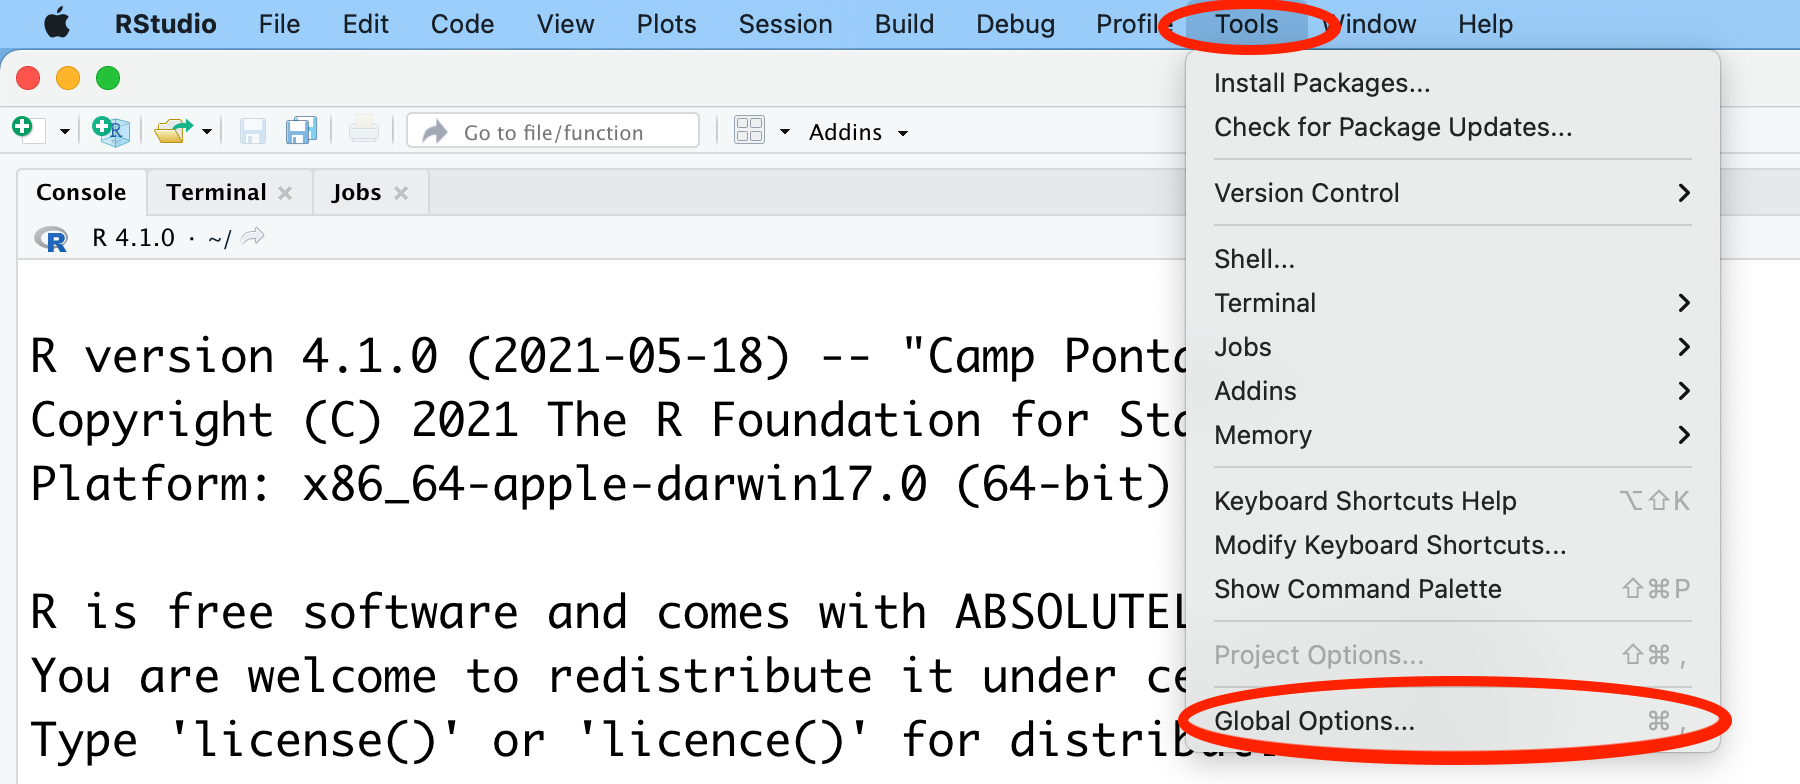
\includegraphics[width=0.9\linewidth]{pics/1font} 

}

\caption{Global Options}\label{fig:font}
\end{figure}

Then, you will see a window popping up like Figure \ref{fig:size}. After clicking on \emph{Appearance}, you can see several drop-down menus including \emph{Zoom} and \emph{Editor font size} among other choices shown.

\begin{itemize}
\item
  \emph{Zoom} controls the overall scale for all elements in the RStudio interface, including the sizes of the menu, buttons, as well as fonts.
\item
  \emph{Editor font size} controls the size of the font only in the code editor.
\end{itemize}

Once done customizing the appearance, you need to click on \emph{Apply} to save the adjustments.

\begin{figure}

{\centering 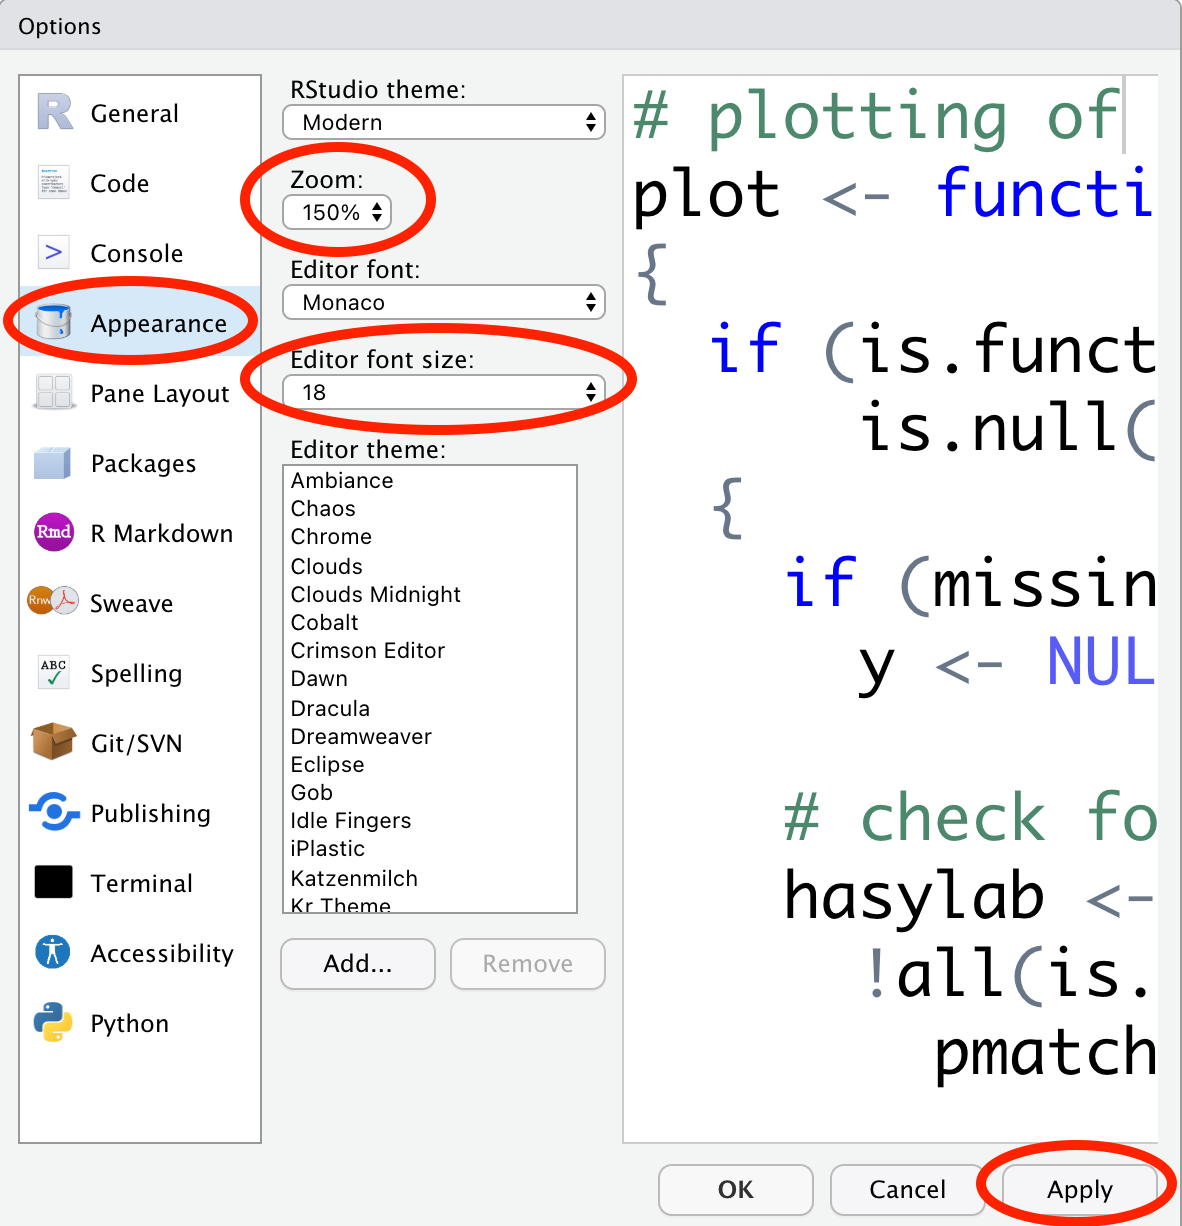
\includegraphics[width=0.7\linewidth]{pics/1size} 

}

\caption{Zoom and Editor font size}\label{fig:size}
\end{figure}

Here, we change the \emph{Zoom} to 150\% and set the \emph{Editor font size} to 18.

\textbf{\emph{b. Four panels of RStudio}}

Now, the RStudio interface is clearer with a bigger font size. Although RStudio has four panels, not all of them are visible to us at the beginning (Figure \ref{fig:open}).

\begin{figure}

{\centering 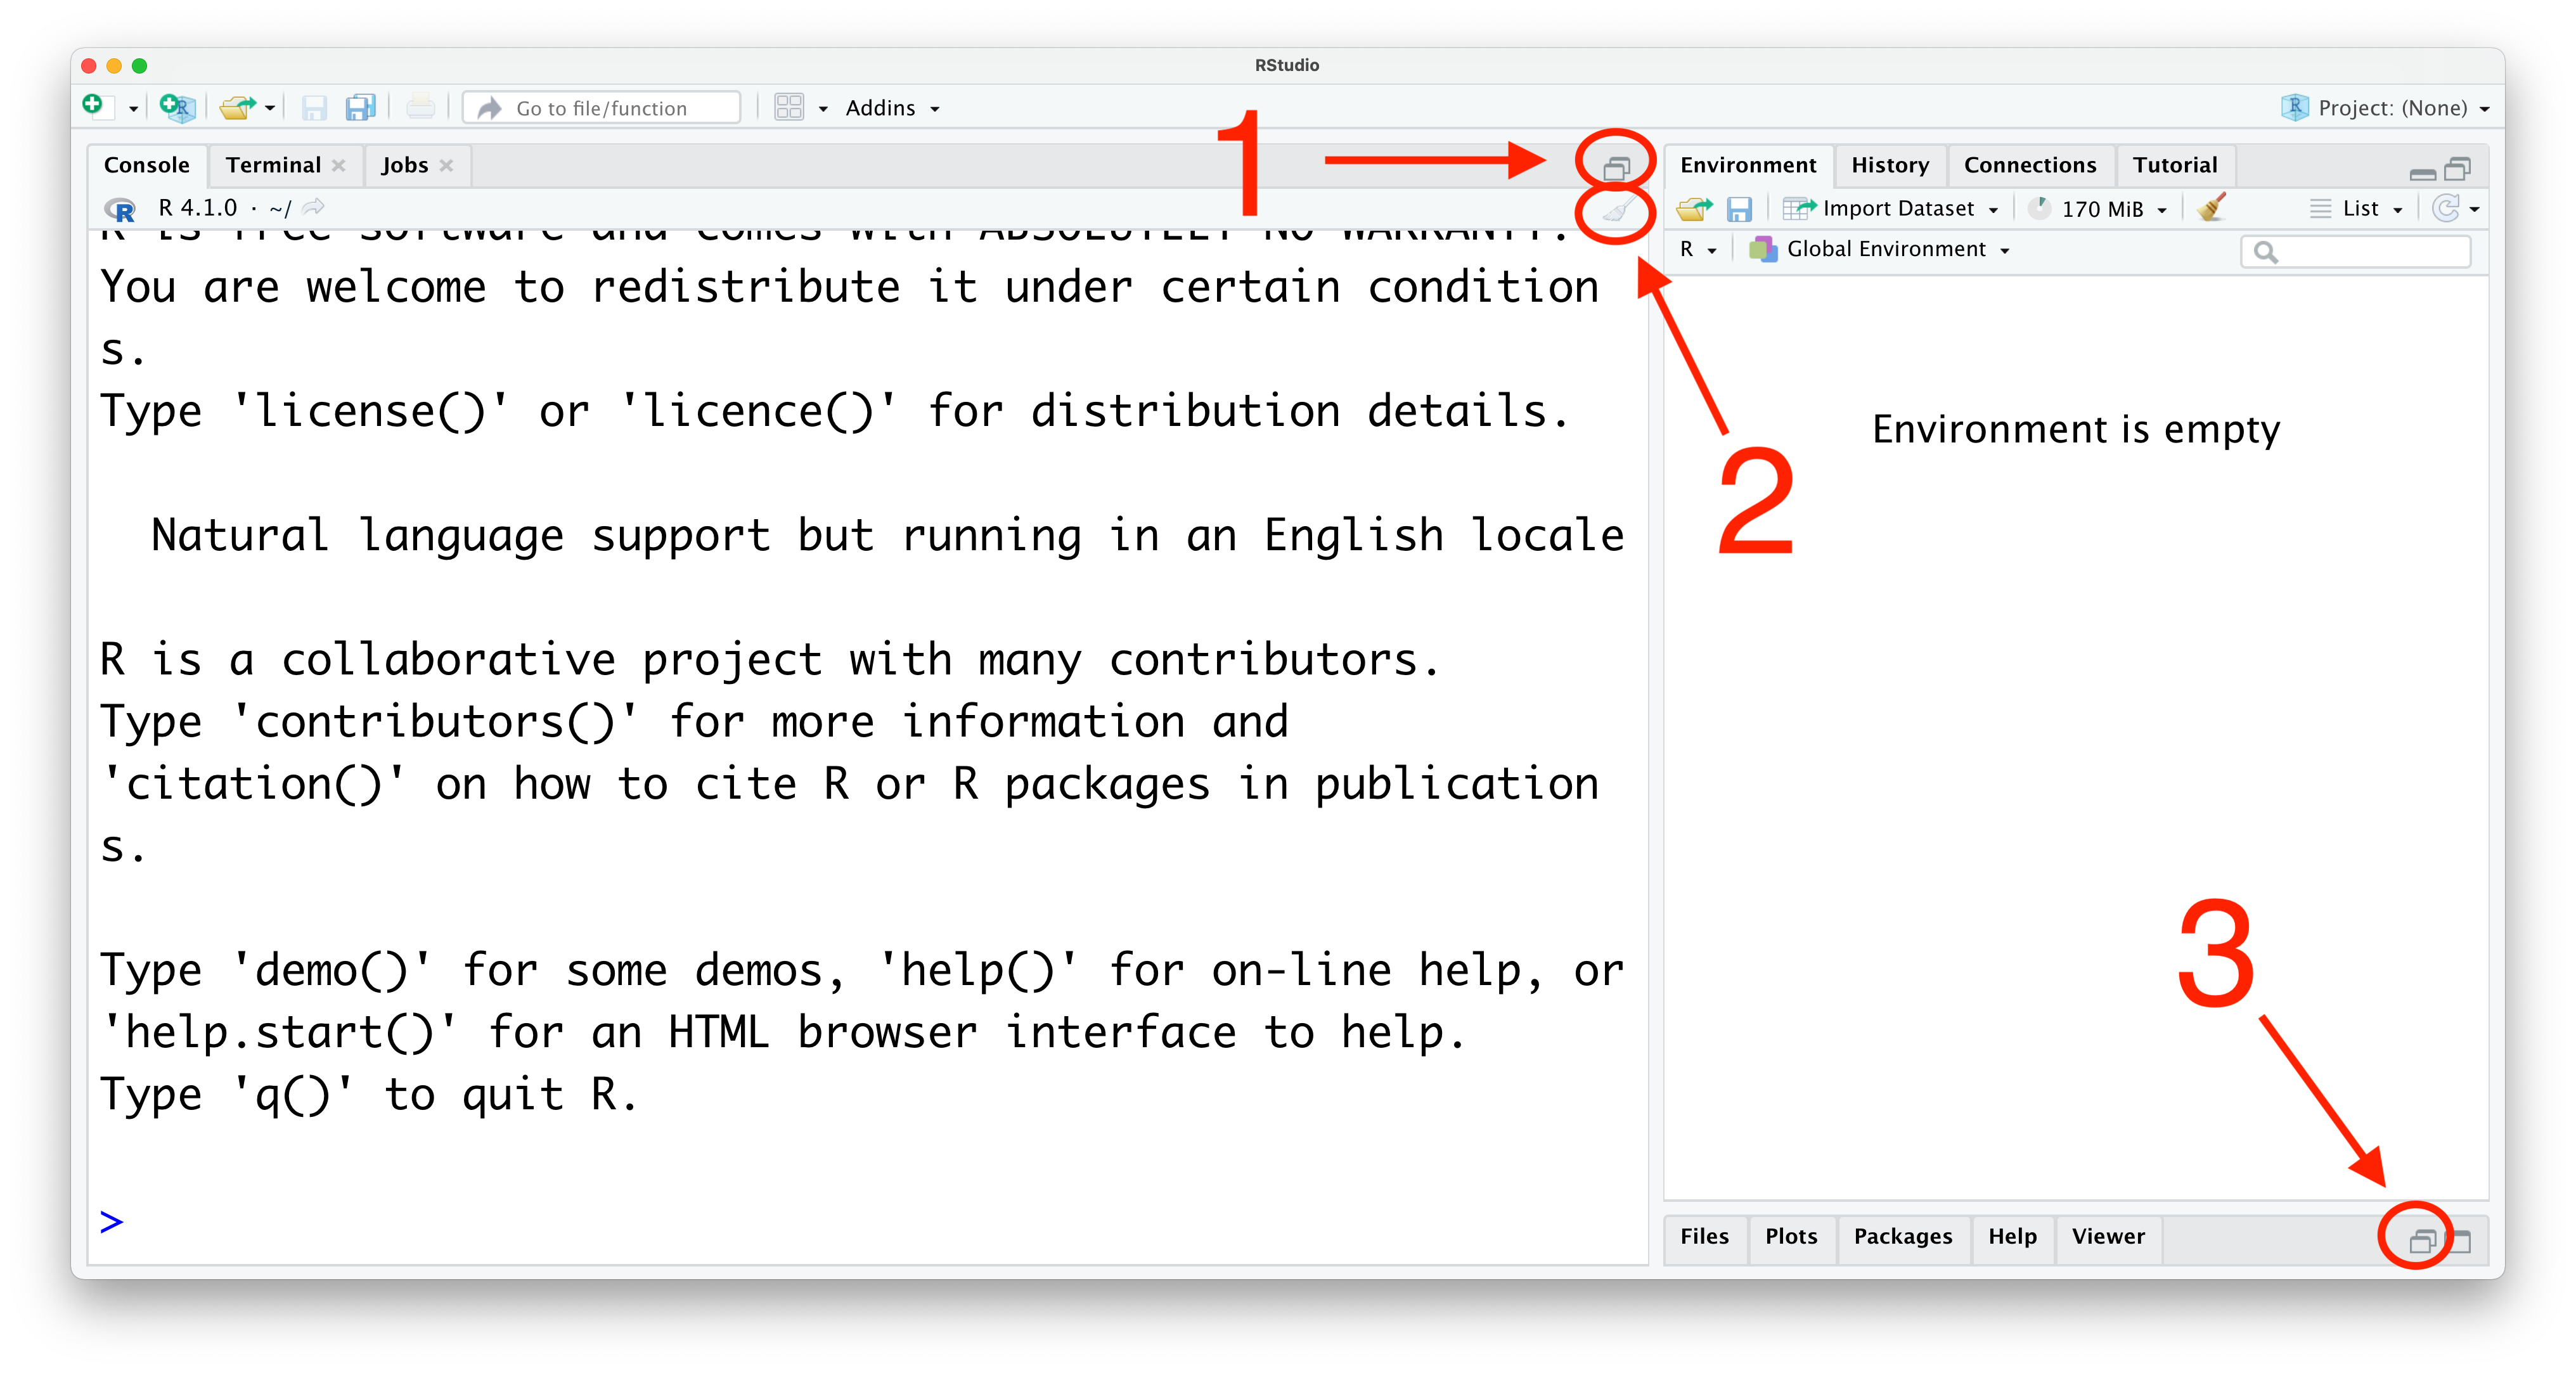
\includegraphics[width=1\linewidth]{pics/1open} 

}

\caption{Unfold panels}\label{fig:open}
\end{figure}

In Figure \ref{fig:open}, we have labeled three useful buttons as 1, 2, and 3. By clicking buttons 1 and 3, you can reveal the two hidden panels.

\begin{infobox}{caution}
Note that you may see different panels hidden when you open RStudio for the first time, depending on the RStudio version. However, you can always reveal the hidden panels by clicking the corresponding buttons like Buttons 1 and 3 in Figure \ref{fig:open}.

\end{infobox}

By clicking button 2, we can clear the content in the bottom left panel (Panel 2 in Figure \ref{fig:four}) as shown in the following figure.

\begin{figure}

{\centering 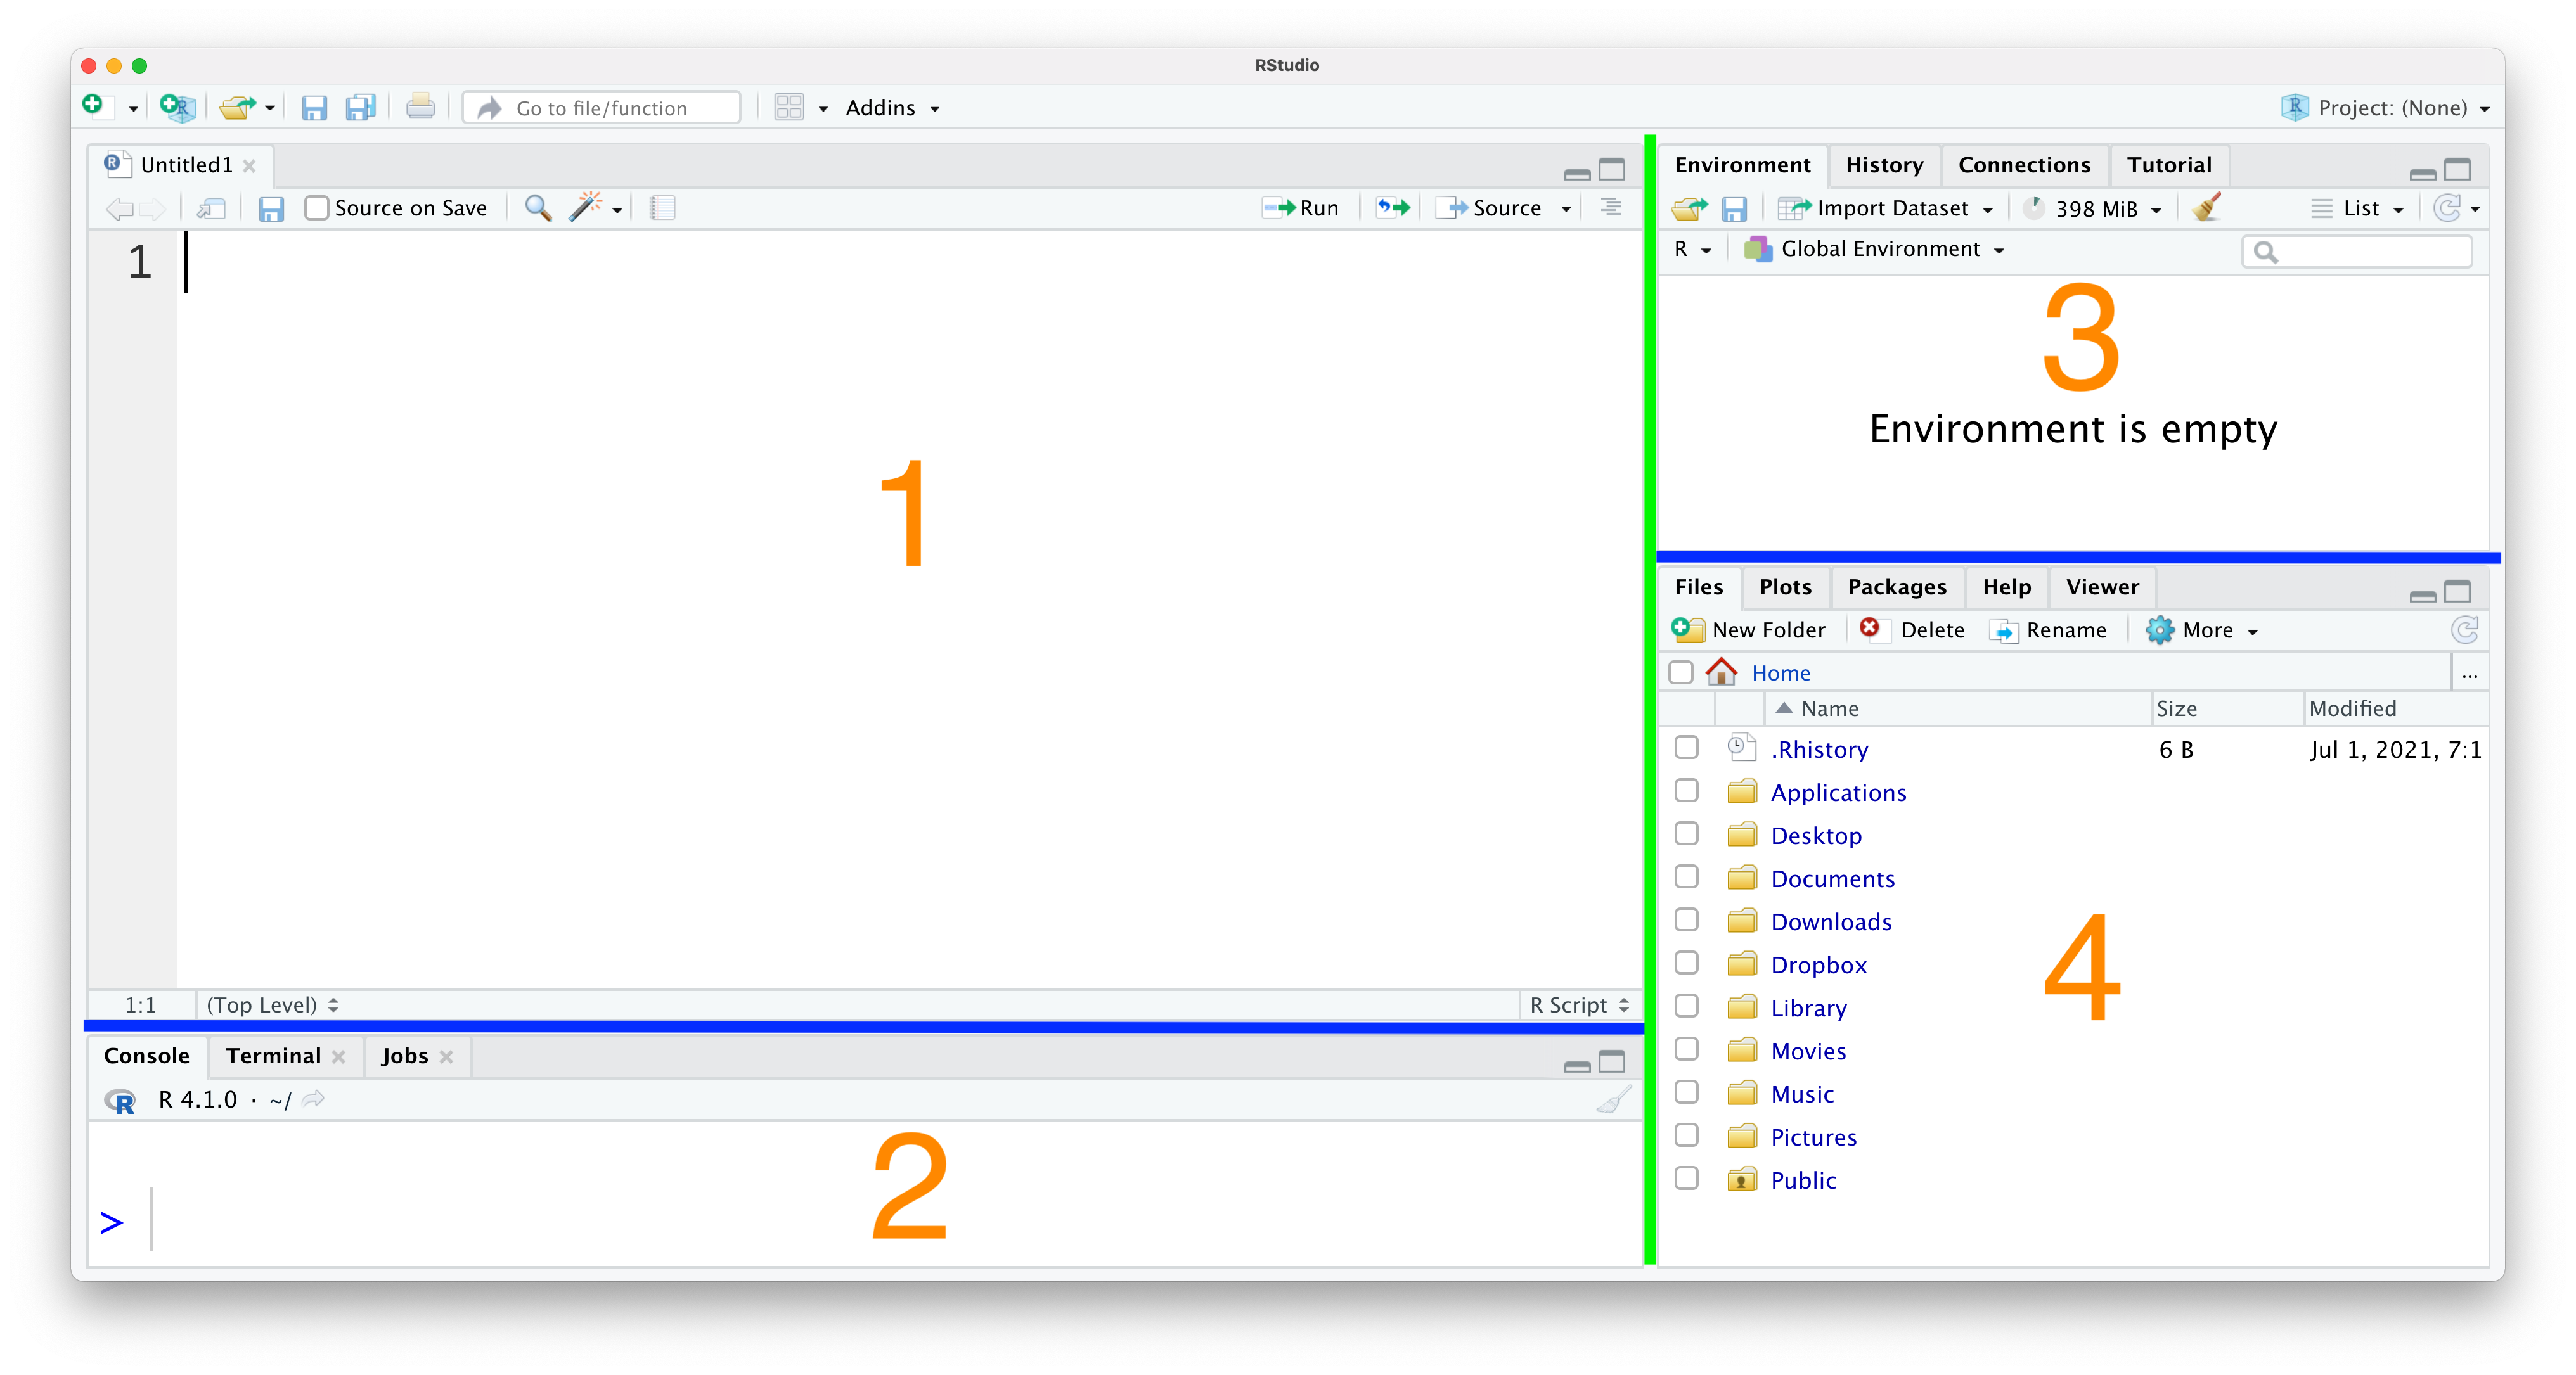
\includegraphics[width=1\linewidth]{pics/1four} 

}

\caption{Four panels}\label{fig:four}
\end{figure}

Now, let's take a close look at all four panels, which are labeled as 1-4 in Figure \ref{fig:four}. You can change the size of each panel by dragging the two blue slides \emph{up} or \emph{down} and the green slide \emph{left} or \emph{right}.

\begin{itemize}
\item
  Located to the left of the green line, Panels 1 and 2 together compose the \textbf{Code Area}. We will introduce them in the following parts of this section.
\item
  Located to the right of the green line, Panels 3 and 4 together make up the \textbf{R Support Area}. We will introduce these two panels in later sections.
\end{itemize}

\textbf{\emph{c.~Console}}

Firstly, we will introduce panel 2 in Figure \ref{fig:four}, which is usually called the \textbf{Console}. The console window is the place for you to type in codes (i.e.~the things you want R to do) and you will get the results immediately once you run the codes.

By clicking the mouse on the line after the \texttt{\textgreater{}} symbol, you can see a blinking cursor, indicating that R is ready to accept codes. Let's type \texttt{1\ +\ 2} and press \emph{Return} (on Mac) or \emph{Enter} (on Windows).

\begin{infobox}{caution}
It is a good habit to add spaces around an operator to increase the readability of the code.

\end{infobox}

\begin{figure}

{\centering 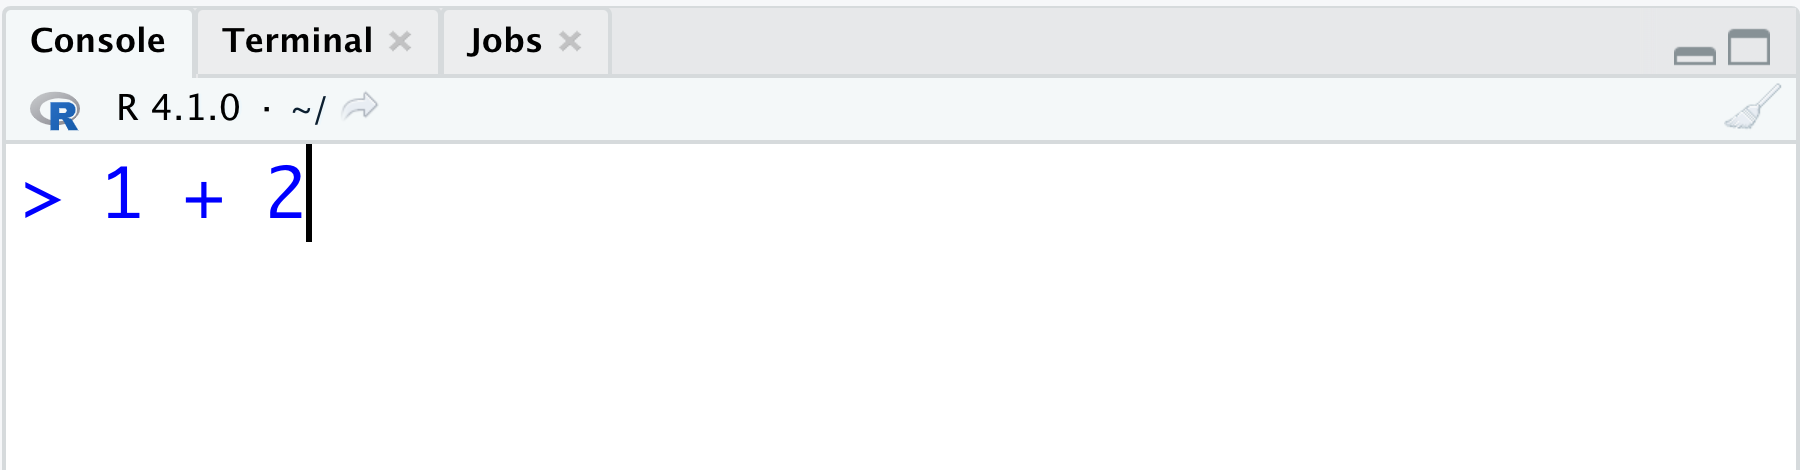
\includegraphics[width=0.7\linewidth]{pics/1code} 

}

\caption{Writing code in the console}\label{fig:code}
\end{figure}

\begin{figure}

{\centering 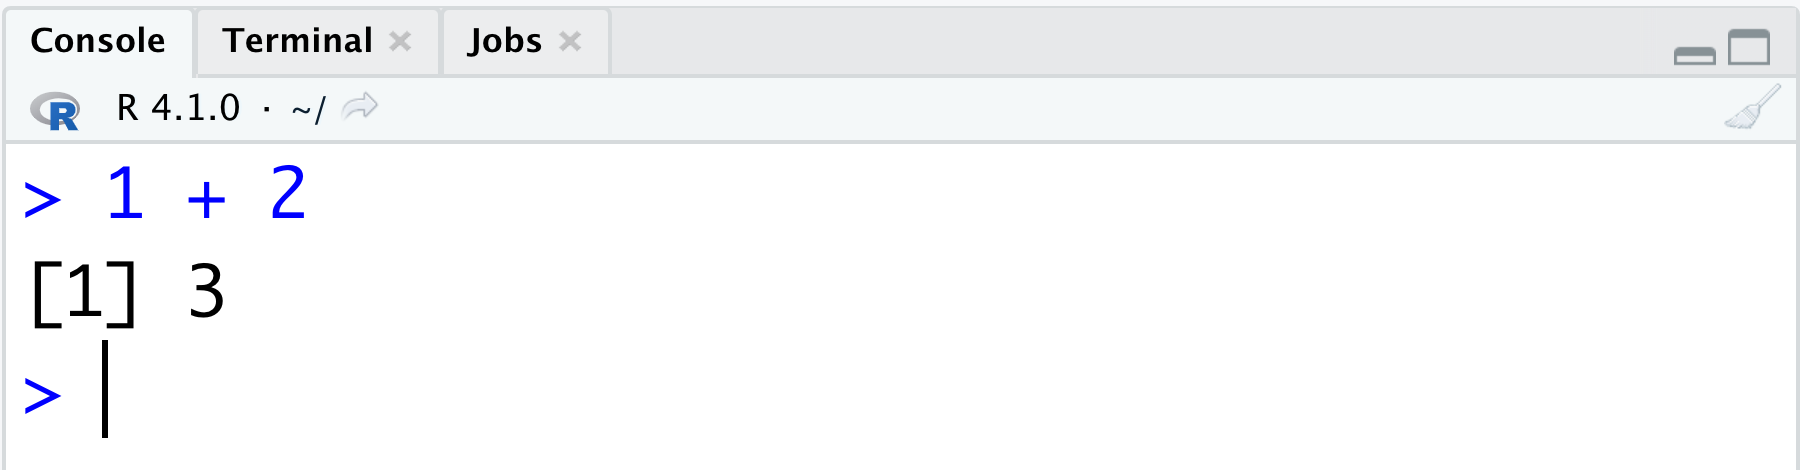
\includegraphics[width=0.7\linewidth]{pics/1answer} 

}

\caption{R code(2)}\label{fig:answer}
\end{figure}

Hooray! You have successfully run the first piece of R code and gotten the correct answer 3. Note that the blinking cursor now appears on the next line, ready to accept a new line of code.

\begin{infobox}{caution}
The curious you may found that there is a \texttt{{[}1{]}} showing before the result \texttt{3}. In fact, the \texttt{{[}1{]}} is an index indicator, showing the next element has an index of 1 in this particular object. We will revisit this point when we introduce vectors in the beginning of Chapter \ref{r-objects} .

\end{infobox}

Although the console may work well for some quick calculations, you need to resort to panel 1 in Figure \ref{fig:four} (known as the \textbf{Editor}) to save our work and run multiple lines of code at once.

\textbf{\emph{d.~Editor}}

The \textbf{Editor} panel is the go-to place to write complicated R codes, which you can save as R files for repeated use in the future. Several kinds of files are available in RStudio. In particular, \textbf{R script}, \textbf{R Markdown}, and \textbf{R Notebook} are the three most common file formats. In order to let you get started better, we will start with R script since this is the simplest file format in R. In Chapter 12 and ??, we will introduce R Markdown and R Notebook in detail.

In the editor panel, you may notice that RStudio has created a file by default (Figure \ref{fig:P1}). The default file RStudio provided is \textbf{R script}.

\begin{figure}

{\centering 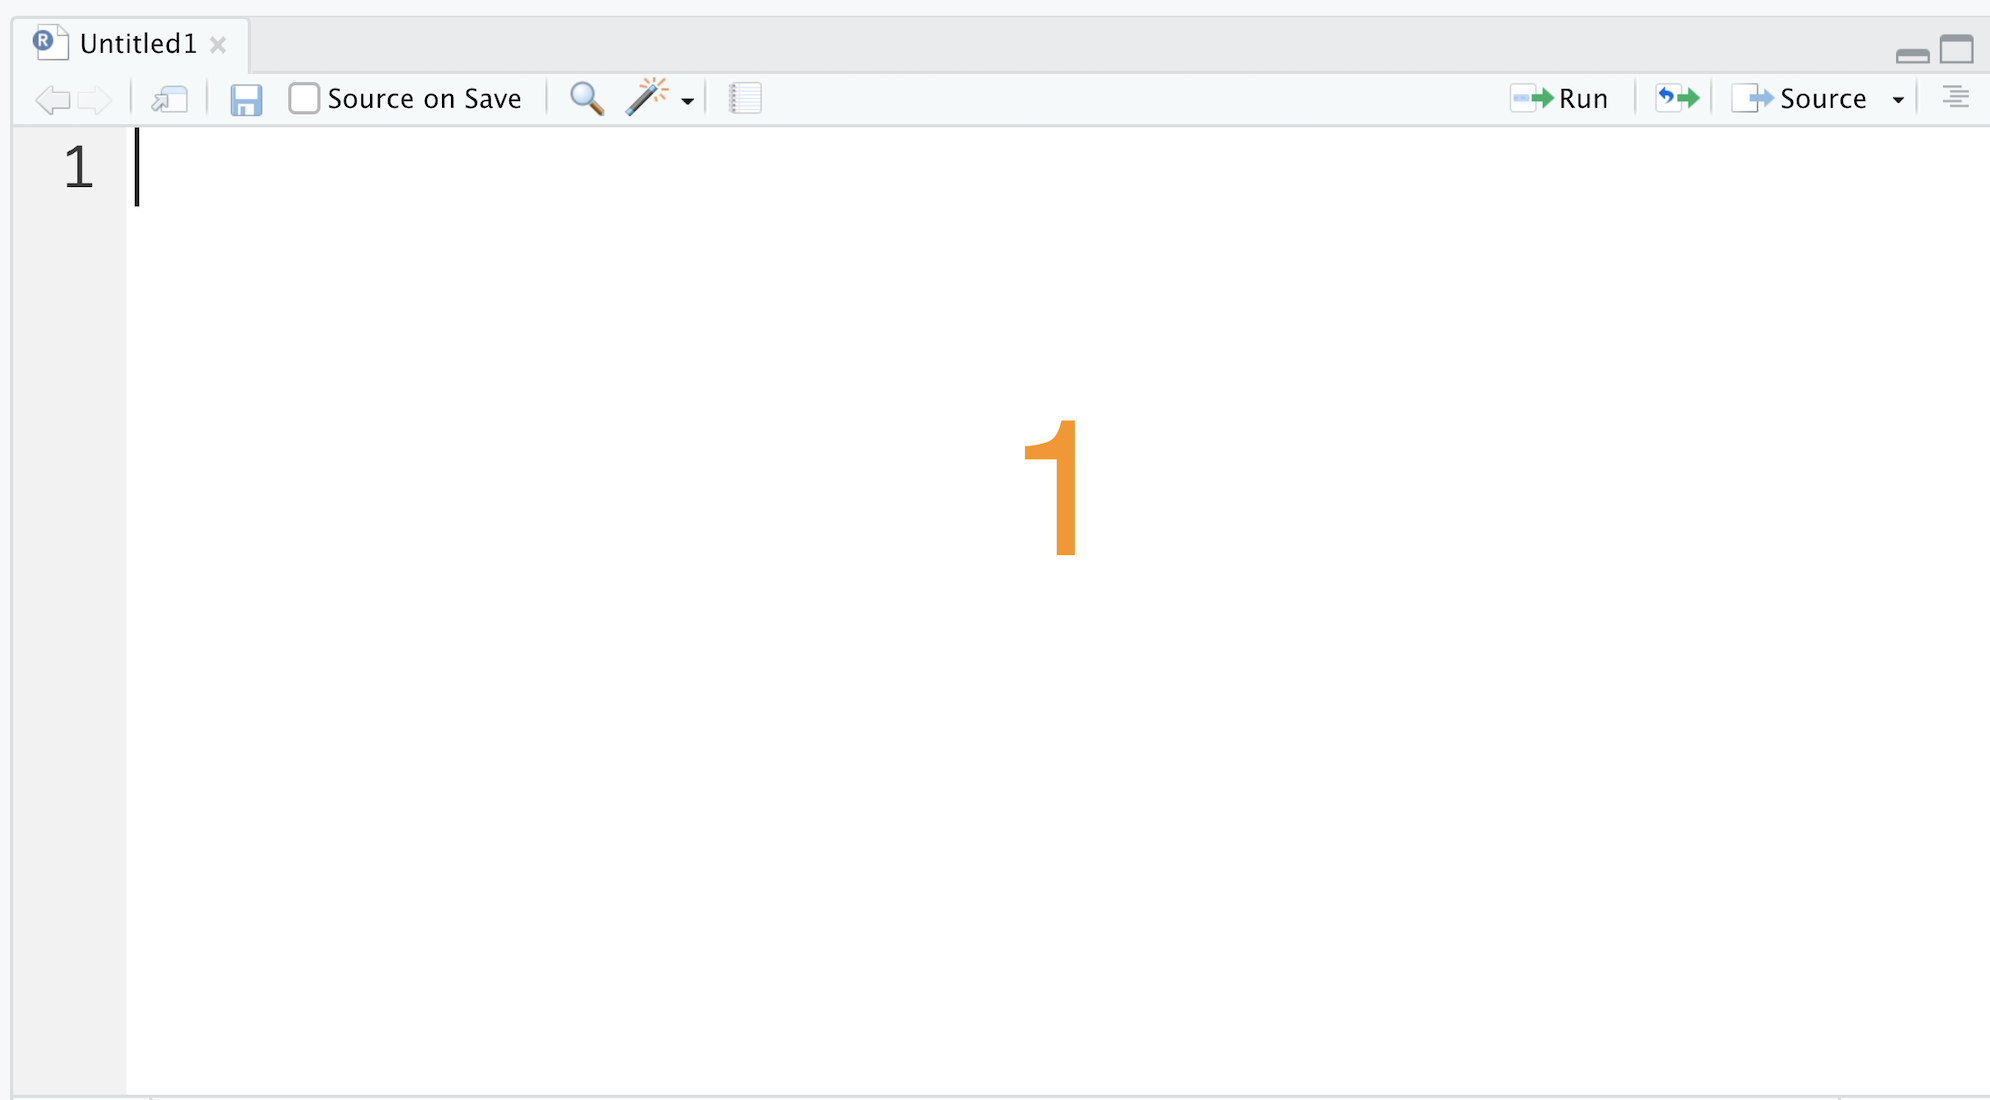
\includegraphics[width=0.7\linewidth]{pics/1P1} 

}

\caption{R script}\label{fig:P1}
\end{figure}

Next, we will introduce how to run codes in scripts. Let's go to the editor and type \texttt{1\ +\ 2}. To run this line of code, you can select this line of code and click the \emph{Run} button. The keyboard shortcut of running this line of code is Cmd+Return on Mac or Ctrl+Enter on Windows. RStudio will then send the line of code to the console and execute the code.

\begin{figure}

{\centering 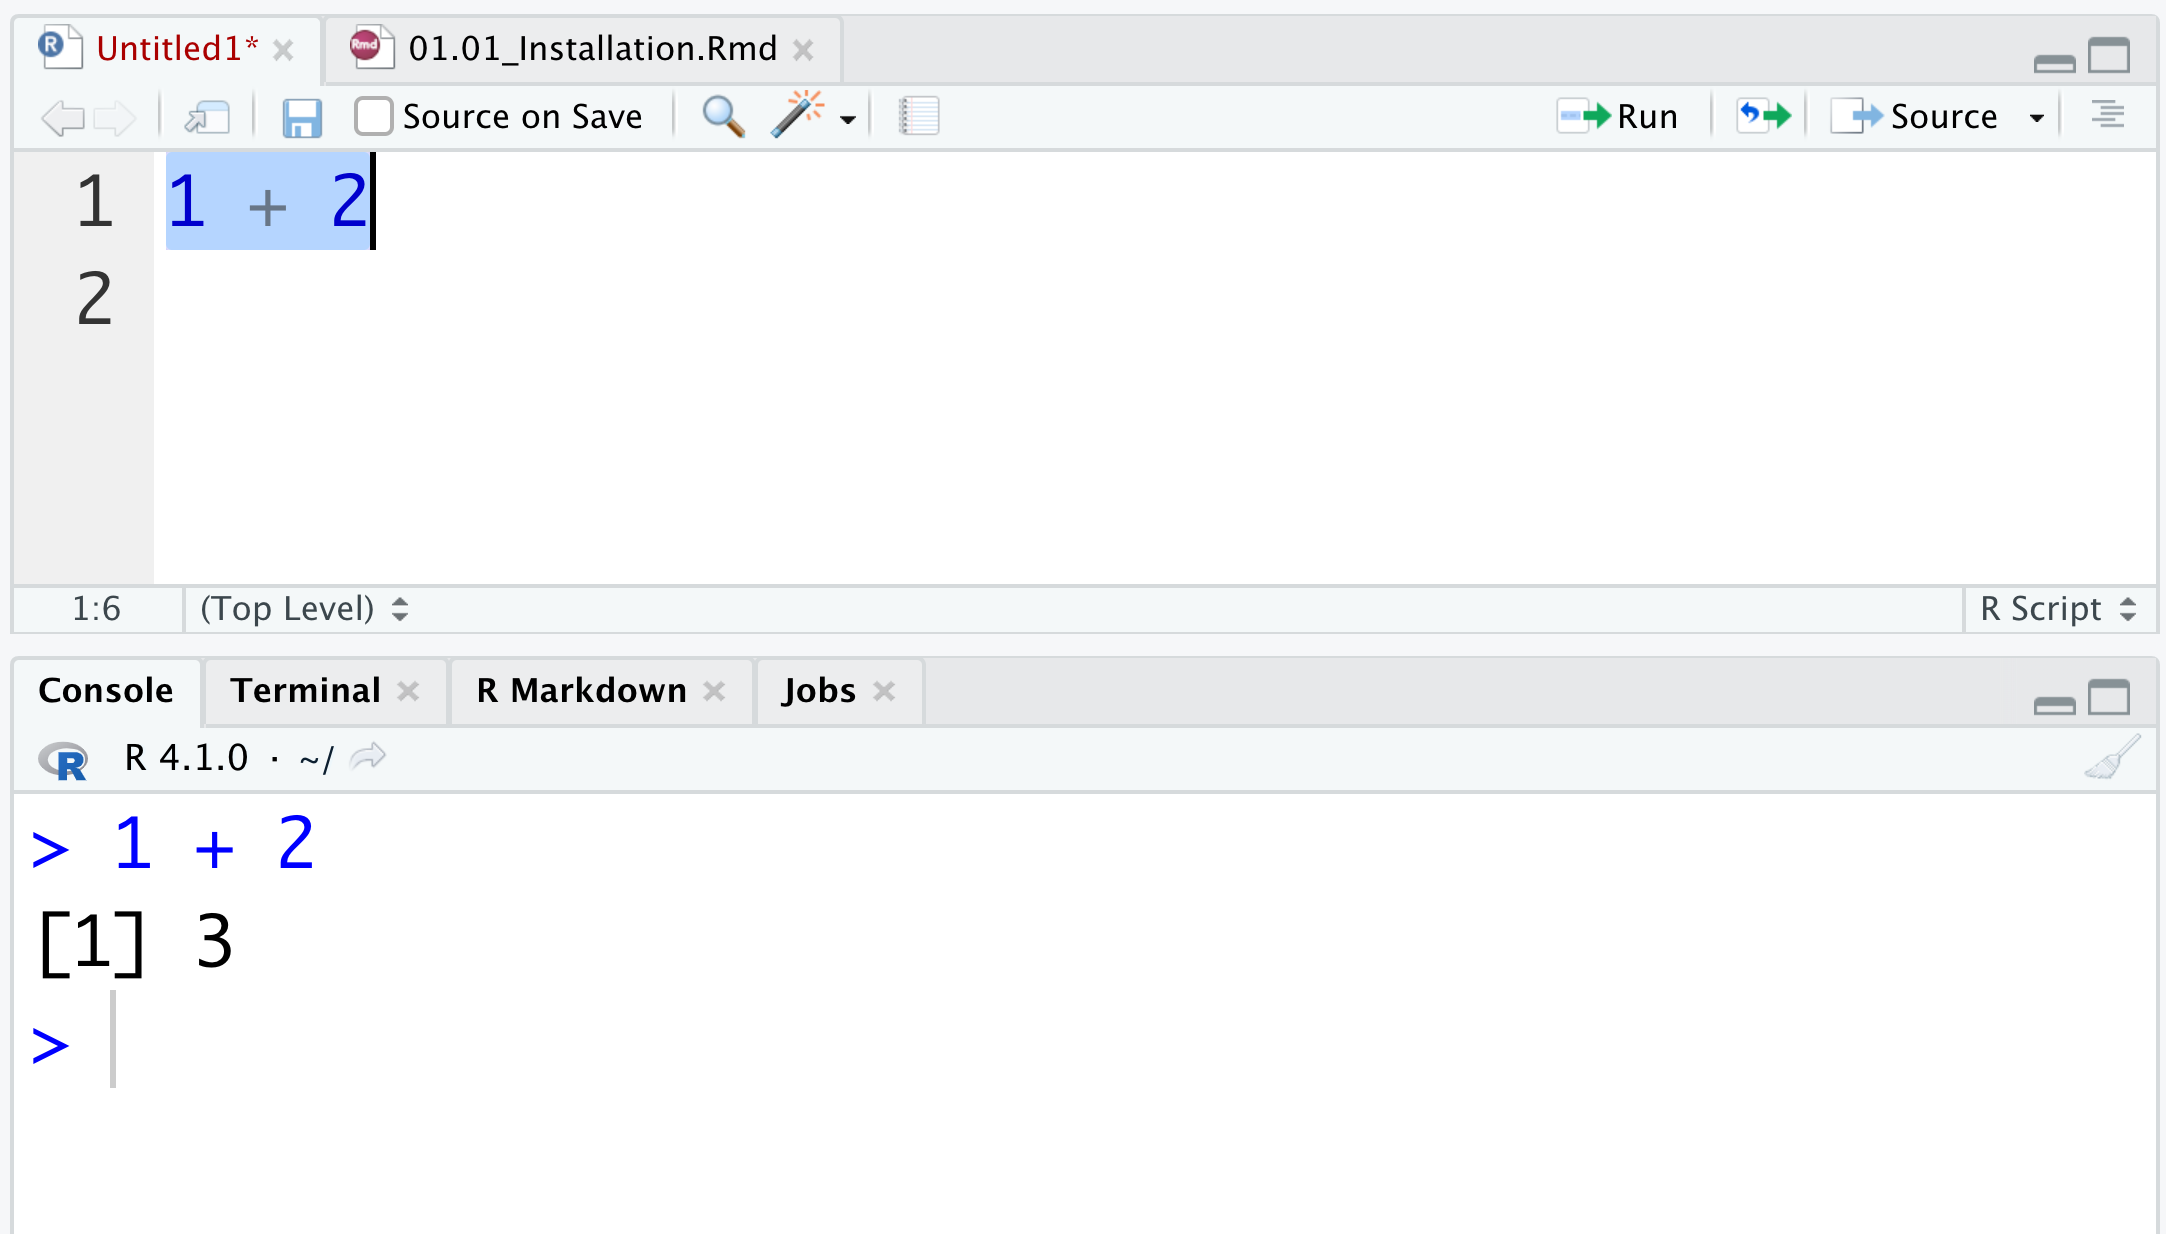
\includegraphics[width=0.7\linewidth]{pics/1run} 

}

\caption{Run codes in script (I)}\label{fig:run}
\end{figure}

You can also run multiple lines of code by selecting the lines and clicking the \emph{Run} button or using the keyboard shortcut. (Figure \ref{fig:mcodes})

\begin{figure}

{\centering 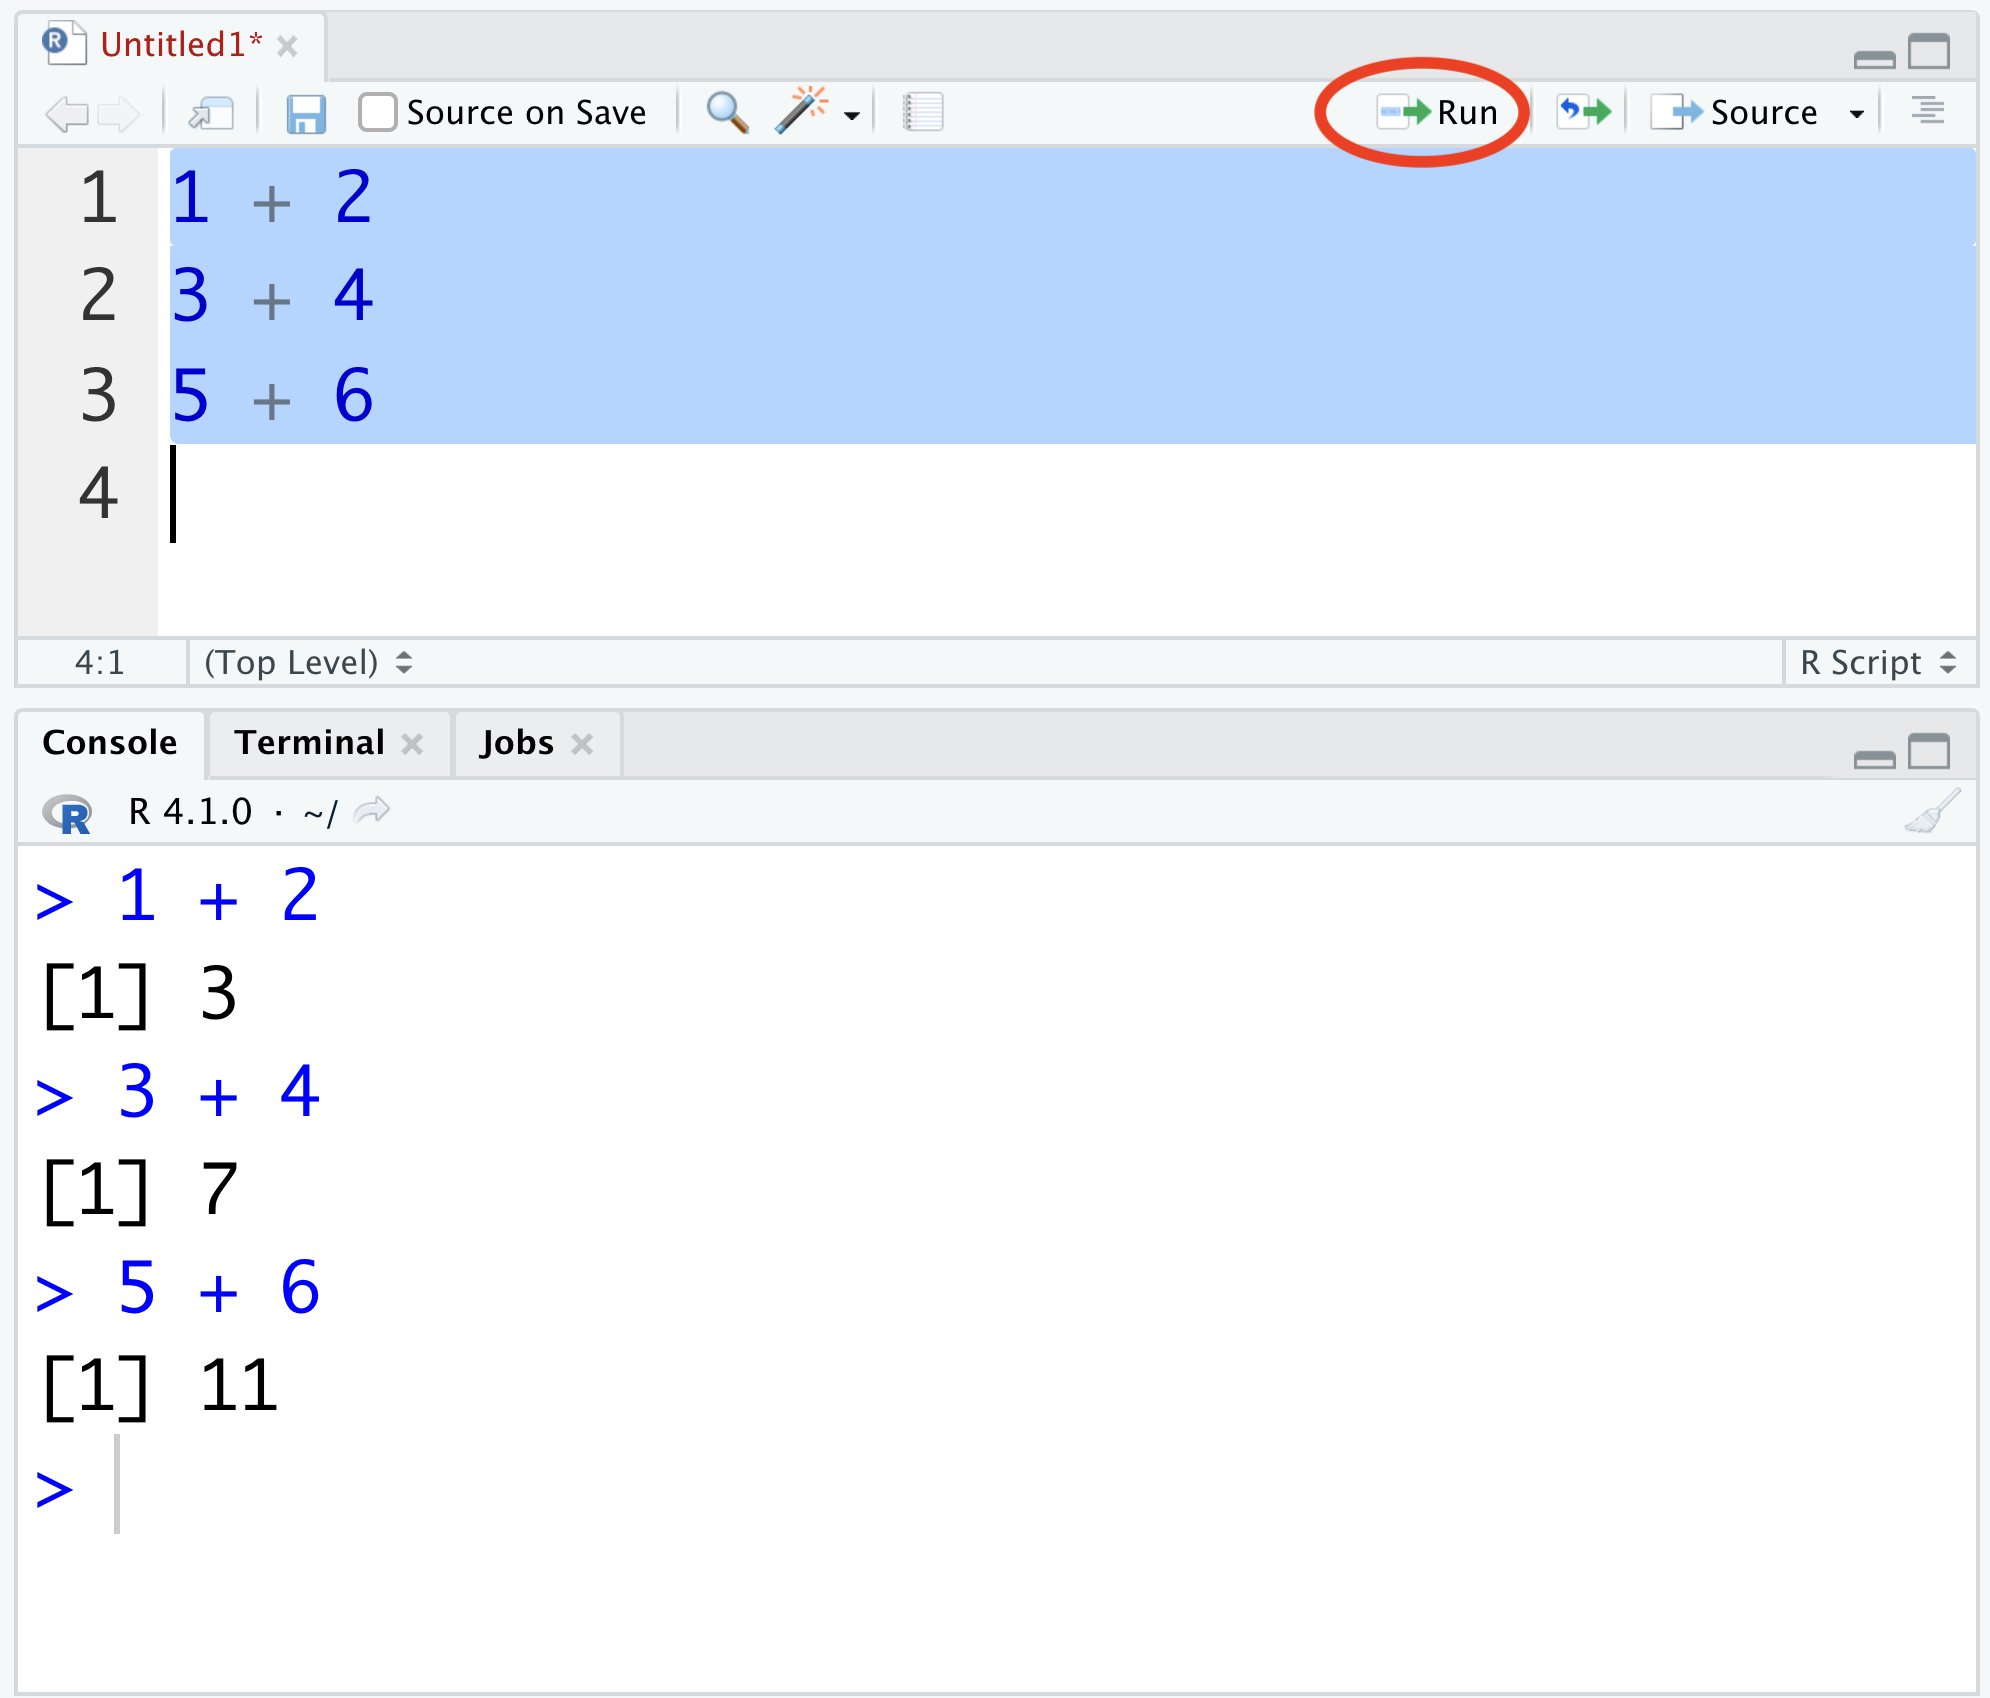
\includegraphics[width=0.7\linewidth]{pics/1mcodes} 

}

\caption{Run codes in script (II)}\label{fig:mcodes}
\end{figure}

Here, three lines of codes are selected. After running these three lines of code together, you can see that the console executes each line of code and you will get the corresponding answer one by one. Therefore, you can write any number of lines of codes in the script, and you can get the answer of each line in the console.

After finishing writing codes in the editor, there may be hundreds or more lines of codes in the script. Now, you may wonder if you need to write these codes again when you want to use the same codes next time. The answer is absolutely NO!!! One of the most important features of R files is that R files can be saved for future use. So do R scripts! To do that, you can click the \emph{Save} button as shown in Figure \ref{fig:save1}. The keyboard shortcut of saving files is Cmd+S on Mac or Ctrl+S on Windows.

\begin{figure}

{\centering 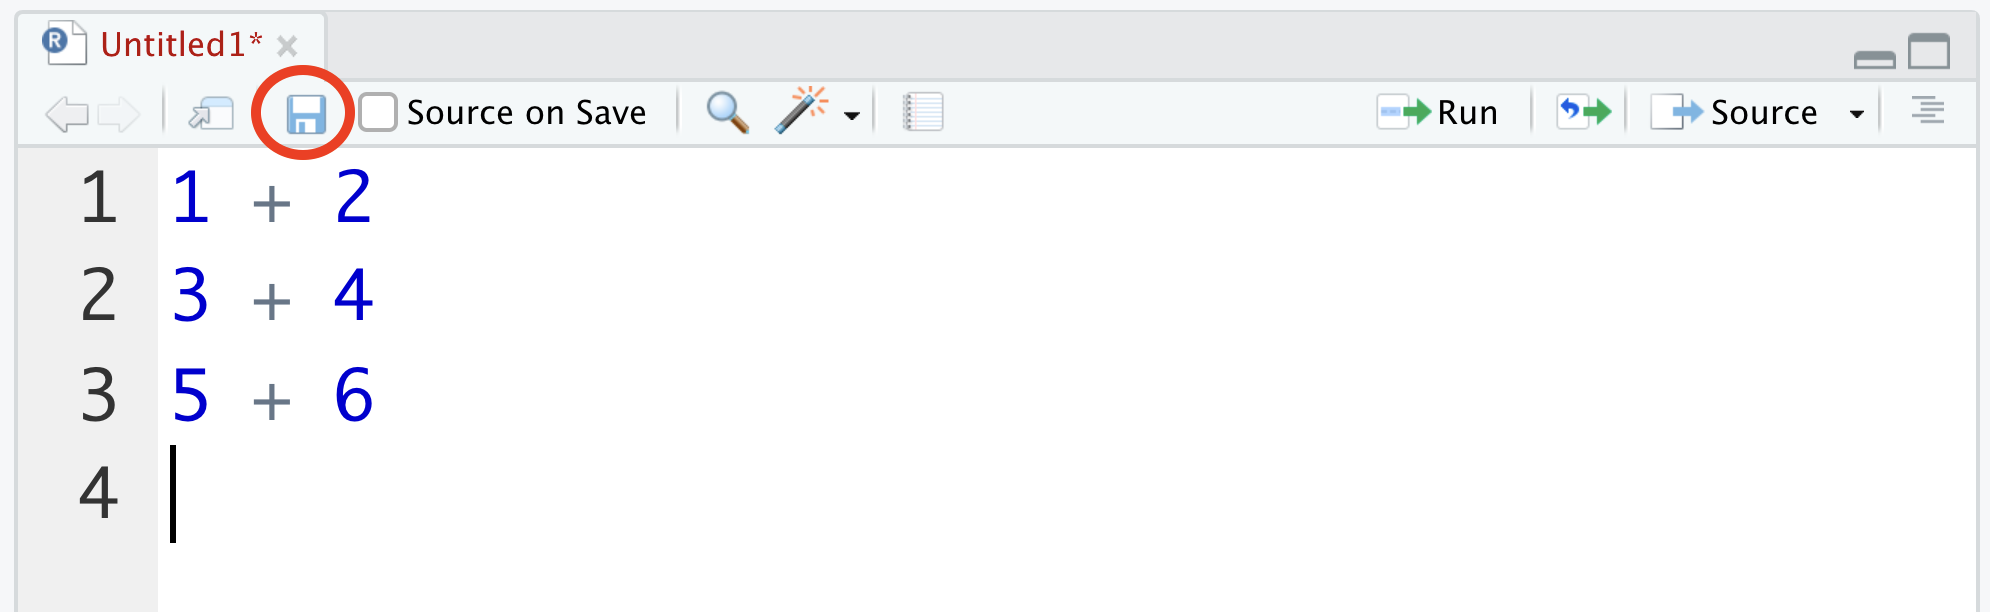
\includegraphics[width=0.7\linewidth]{pics/1save1} 

}

\caption{Save (I)}\label{fig:save1}
\end{figure}

Then you would see a pop-up file dialog box, asking you for a file name and location to save it to. Let's call it lesson1.1 here.

\begin{figure}

{\centering 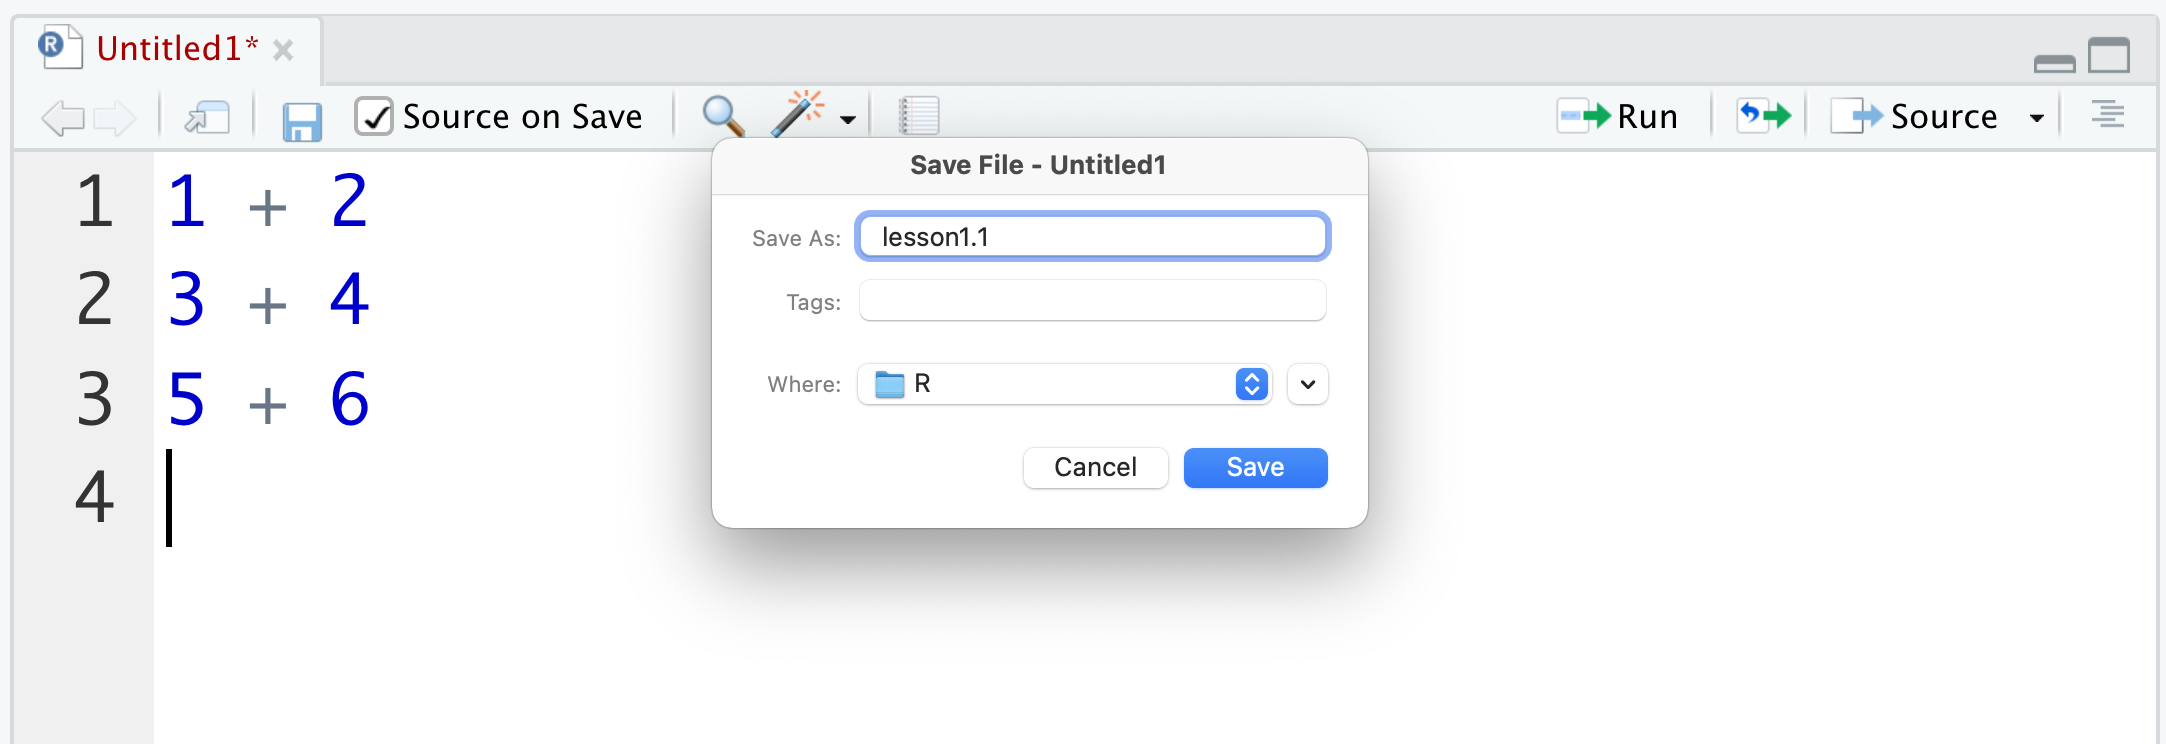
\includegraphics[width=0.7\linewidth]{pics/1save2} 

}

\caption{Save (II)}\label{fig:save2}
\end{figure}

After saving files successfully, you can confirm the name of the R script on the top.

\begin{figure}

{\centering 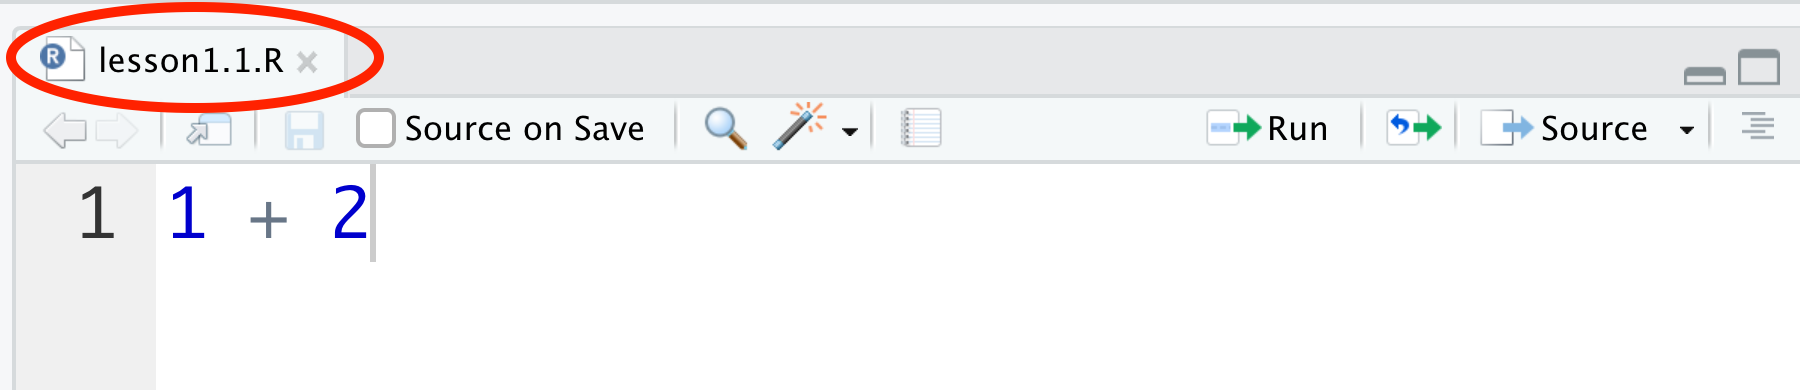
\includegraphics[width=0.7\linewidth]{pics/1save3} 

}

\caption{Save (III)}\label{fig:save3}
\end{figure}

Then if you close this script and open it again, you would directly see the previous three lines of codes without writing them again.

Lastly, if you want to create a new R script, you can click the \texttt{+} button on the menu, then select \emph{R Script}. Note that there are quite a few other options including \emph{R Markdown}, which will be introduced in Chapter \ref{r-markdown}.

\begin{figure}

{\centering 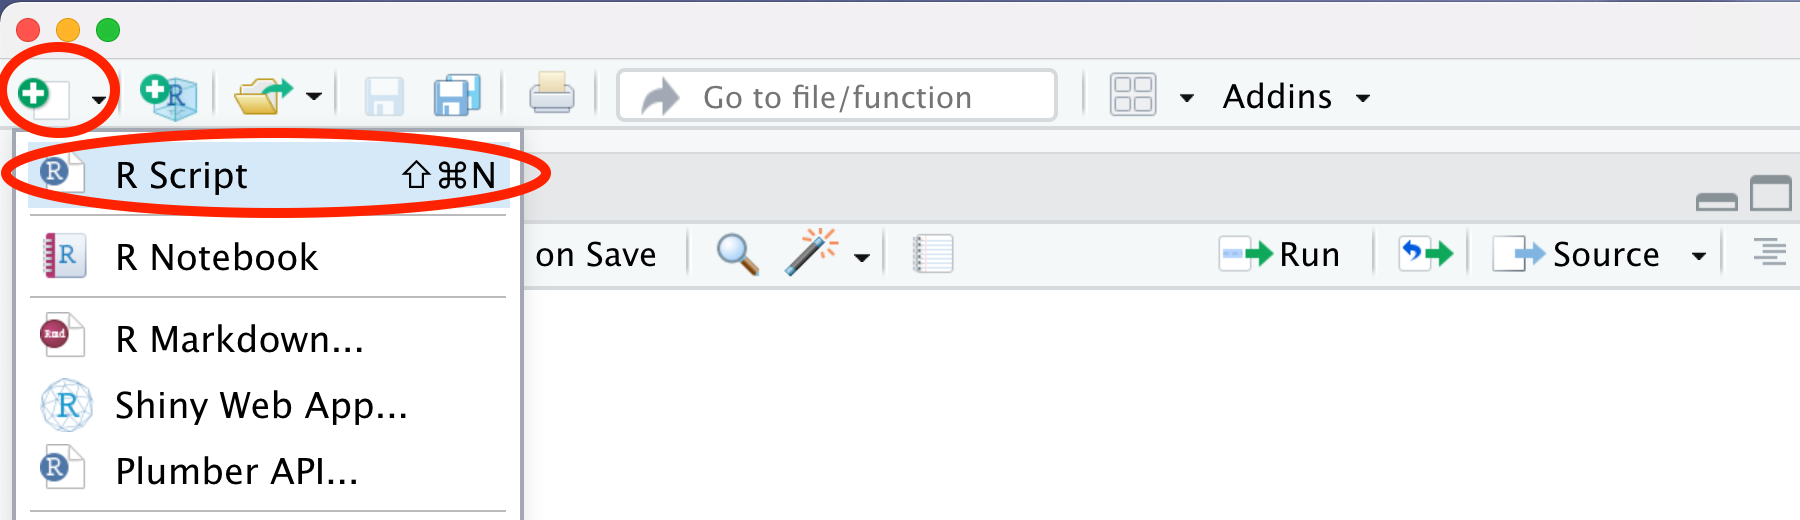
\includegraphics[width=0.7\linewidth]{pics/1new} 

}

\caption{create a new script (I)}\label{fig:new}
\end{figure}

Consequently, you will see a new file created.

\begin{figure}

{\centering 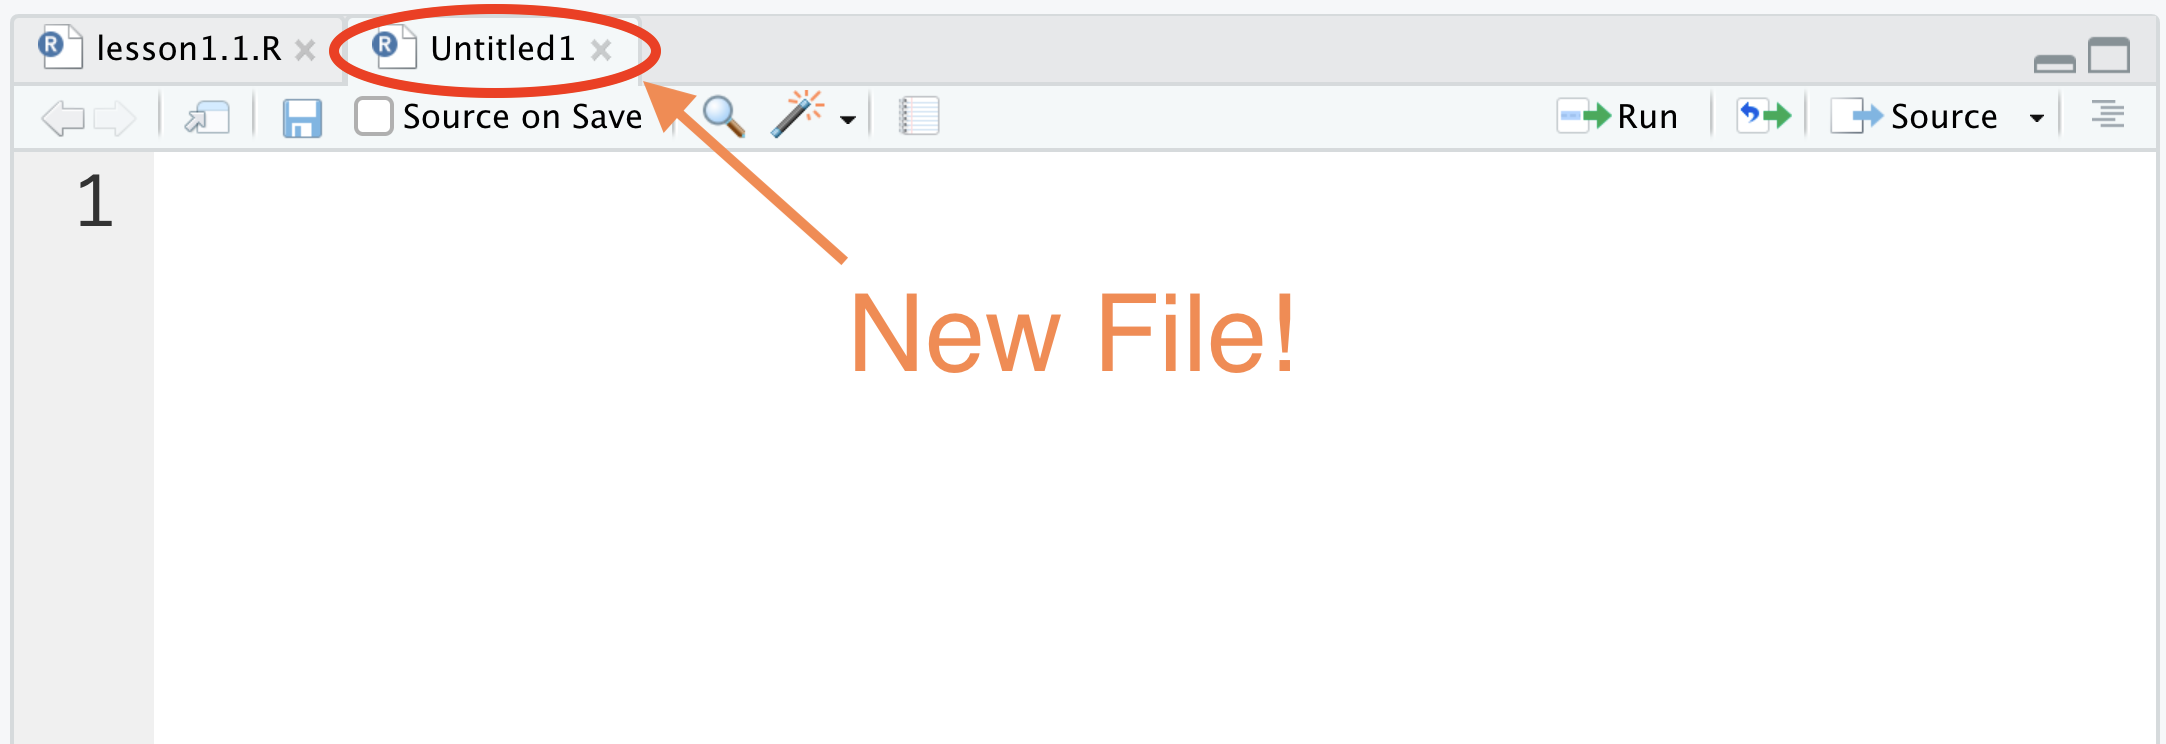
\includegraphics[width=0.7\linewidth]{pics/1new2} 

}

\caption{create a new script (II)}\label{fig:new2}
\end{figure}

\hypertarget{install-and-load-r-packages}{%
\subsection{Install and load R packages}\label{install-and-load-r-packages}}

Now, you have had a basic understanding of RStudio, it is time to meet \textbf{R packages}, which greatly extend the capabilities of base R. There are a large number of publicly available R packages. As of July 2021, there are more than 17K R packages on Comprehensive R Archive Network (CRAN), with many others located in Bioconductor, GitHub, and other repositories.

To install an R package, you need to use a built-in R \textbf{function}, which is \texttt{install.packages()}. A \textbf{function} takes in \textbf{arguments} (inputs) and performs a specific task accordingly. After the function name, we always need to put \textbf{a pair of parentheses} with the arguments inside.

While there are many built-in R functions, R packages usually contain many useful functions as well, and we can also write our own functions, which will be introduced in Chapter \ref{write-code}.

With \texttt{install.packages()}, the argument is the package name with \textbf{a pair of quotation marks} around it. The task it performs is installing the specific package into R. Here, you will install the companion package for this book, named \texttt{r02pro}, a.k.a. \emph{R Zero to Pro}. The \texttt{r02pro} package contains several data sets that will be used throughout the book, and interactive exercises for each subsection.

\begin{Shaded}
\begin{Highlighting}[]
\FunctionTok{install.packages}\NormalTok{(}\StringTok{"r02pro"}\NormalTok{)}
\end{Highlighting}
\end{Shaded}

\begin{infobox}{caution}
If you miss the right parenthesis, R will return a plus in the next line (as shown in Figure \ref{fig:right1}), waiting for more input to complete the command. If this happens, you can either enter the right parenthesis, or press ESC to escape this command. When you see a blinking cursor after the \texttt{\textgreater{}} symbol, you can write new codes again.

\end{infobox}

\begin{figure}

{\centering 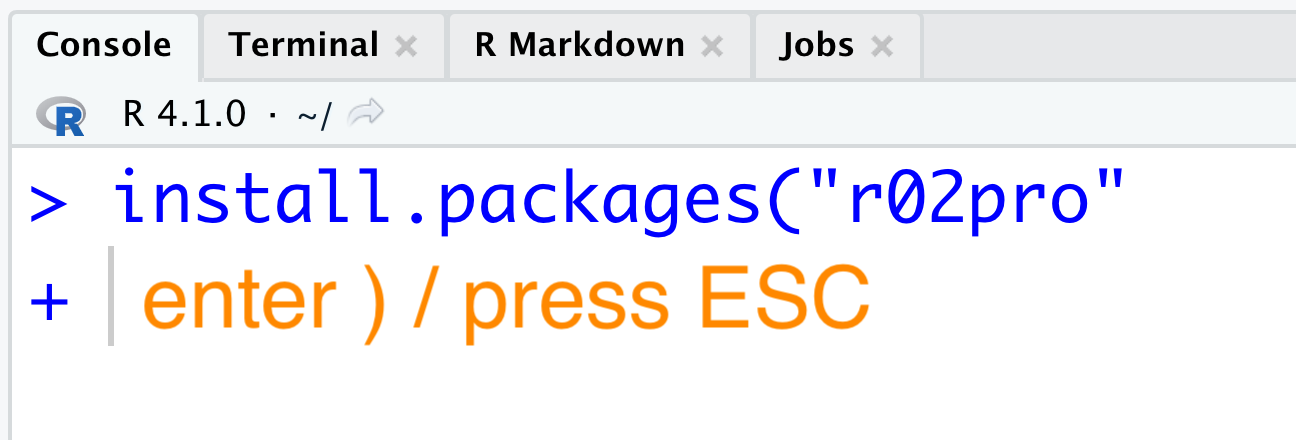
\includegraphics[width=0.7\linewidth]{pics/1right} 

}

\caption{Miss the right parenthesis}\label{fig:right1}
\end{figure}

After a package is installed, you still need to load it into R before using it. To load a package, you can use the \texttt{library()} function with the package name as its argument. Here, quotation marks are not necessary.

\begin{Shaded}
\begin{Highlighting}[]
\FunctionTok{library}\NormalTok{(r02pro)}
\end{Highlighting}
\end{Shaded}

Note that once a package is installed, you \textbf{don't need to} install it again on the same machine. However, when starting a new R session, you would need to load the package again.

\begin{infobox}{caution}

Quotation marks are necessary for installing R packages, but are not necessary for loading packages. When installing packages without quotation marks, you will see an error message, showing \emph{object not found}.

\begin{Shaded}
\begin{Highlighting}[]
\FunctionTok{install.packages}\NormalTok{(r02pro)}
\end{Highlighting}
\end{Shaded}

\end{infobox}

\hypertarget{exercises}{%
\subsection{Exercises}\label{exercises}}

\begin{enumerate}
\def\labelenumi{\arabic{enumi}.}
\tightlist
\item
  Which of the following code used to install packages into R will return an error?
\end{enumerate}

\begin{itemize}
\tightlist
\item
  \texttt{install.packages("r02pro")}
\item
  \texttt{install.packages(r02pro)}
\end{itemize}

\begin{enumerate}
\def\labelenumi{\arabic{enumi}.}
\setcounter{enumi}{1}
\item
  Write the R code to load the package \textbf{r02pro}
\item
  Write the R code to calculate \texttt{2\ +\ 3}.
\end{enumerate}

\hypertarget{Calculator}{%
\section{Use R as a Fancy Calculator}\label{Calculator}}

After learning how to run codes in R, we will introduce how to use R as a fancy calculator.

\hypertarget{add-comments-using}{%
\subsection{Add comments using ``\#''}\label{add-comments-using}}

Before we get started, the first item we will cover is adding comments for codes. In R, you can use the hash character \texttt{\#} at any position of a given line to initiate a comment, and anything after \texttt{\#} will be ignored by R. Let's see an example,

\begin{Shaded}
\begin{Highlighting}[]
\DecValTok{6} \SpecialCharTok{{-}} \DecValTok{1} \SpecialCharTok{/} \DecValTok{2} \CommentTok{\# first calculate 1/2=0.5, then 6{-}0.5=5.5}
\CommentTok{\#\textgreater{} [1] 5.5}
\end{Highlighting}
\end{Shaded}

By running this line of code (either in the console or in the editor!), you will get a value of 5.5, which is the answer of \texttt{6\ -\ 1\ /\ 2}. As demonstrated, R will not run syntax after the hash character \texttt{\#}. Commands and strings after the \texttt{\#} are notations or explanations that can make codes easier to understand. Here, the comment informs you the operation order of previous code: the division is calculated before the subtraction.

In general, adding comments to codes is a very good practice, as it greatly increases readability and make collaboration easier. We will also add necessary comments in our codes to help you learn R.

\hypertarget{basic-calculation}{%
\subsection{Basic calculation}\label{basic-calculation}}

Now let's start to use R as a calculator! In the previous section we introduced operations such as addition, subtraction, multiplication, division, as well as the combination of multiple basic operations. Additionally, you can also calculate the square root, absolute value and the sign of a number.

\begin{tabular}{l|l}
\hline
Operation & Explanation\\
\hline
1 + 2 & addition\\
\hline
1 - 2 & subtraction\\
\hline
2 * 4 & multiplication\\
\hline
2 / 4 & division\\
\hline
6 - 1 / 2 & multiple operations\\
\hline
sqrt(100) & square root\\
\hline
abs(-3) & absolute value\\
\hline
sign(-3) & sign\\
\hline
\end{tabular}

\hypertarget{get-help-in-r}{%
\subsection{Get help in R}\label{get-help-in-r}}

While the first seven operations in the above table look intuitive, you may be wondering, what does the \texttt{sign()} function mean there? Is that a stop sign?

\begin{center}
\includegraphics[width=0.16\linewidth]{pics/1stop} \end{center}

Sometimes, you may have no idea how a particular function works. Fortunately, R provides a detailed documentation for each function.

\textbf{\emph{a. Ask for help}}

First, we will introduce how to ask for help in R, and below are three common ways to seek for more information.

\begin{itemize}
\tightlist
\item
  Use a question mark followed by the function name, e.g.~\texttt{?sign}\\
\item
  Use help function, e.g.~\texttt{help(sign)}
\item
  Use the help window in RStudio, as shown in Figure \ref{fig:help}. The help window is the panel 4 of Figure \ref{fig:four} in Section \ref{Installation}. Then type in the function name in the box to the right of the magnifying glass and press return.
\end{itemize}

\begin{figure}

{\centering 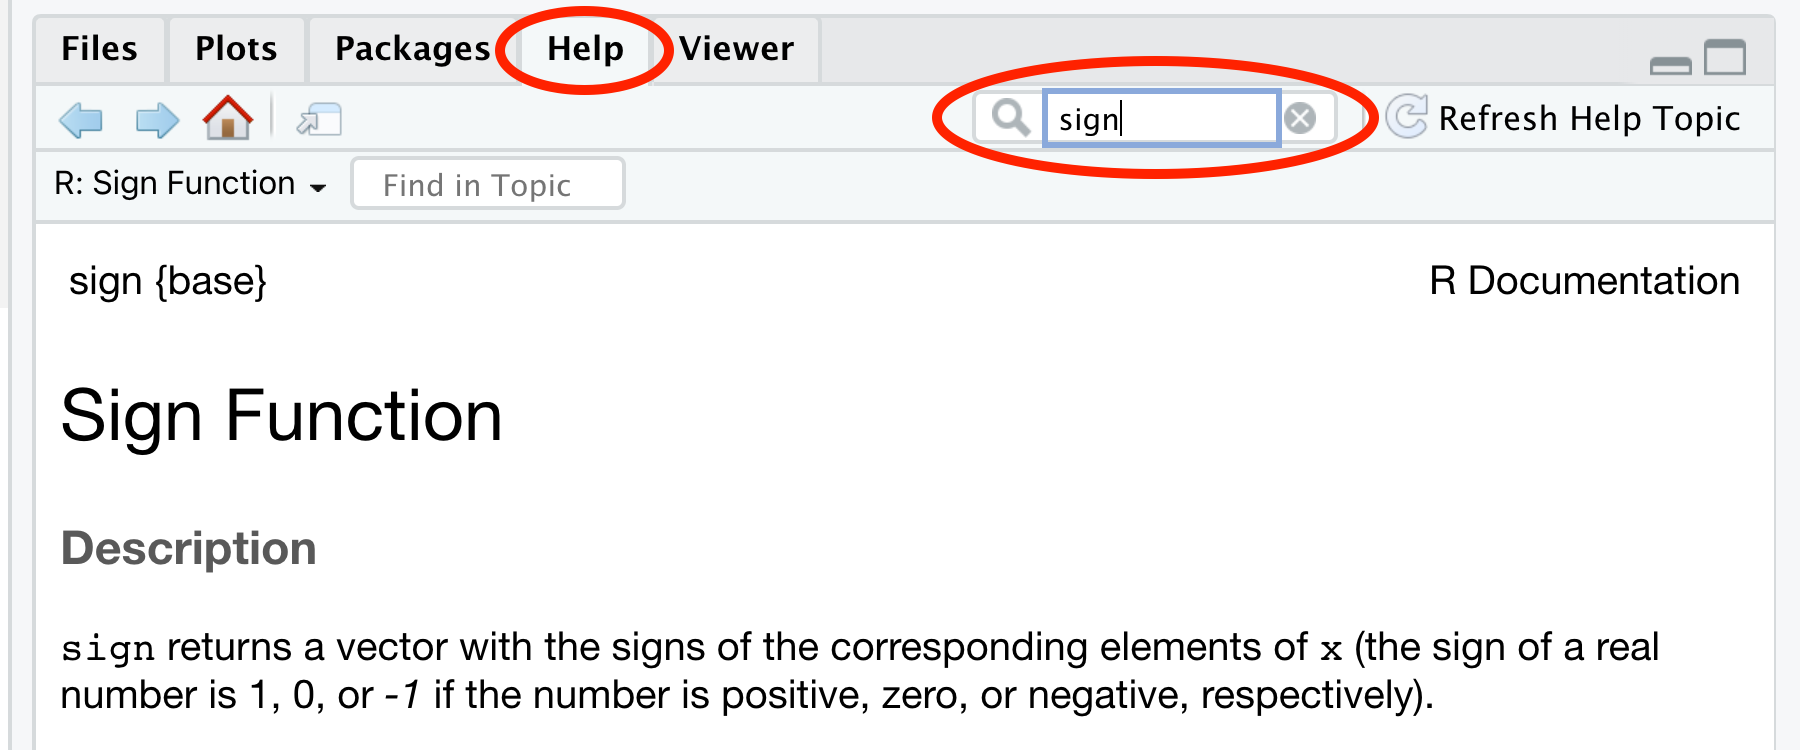
\includegraphics[width=0.7\linewidth]{pics/1help} 

}

\caption{Ask for help}\label{fig:help}
\end{figure}

\textbf{\emph{b. Documentation for functions}}

After using the above operations to ask for help in R, you can get the documentation of the function in the help window. The documentation consists of different parts, let's take the \texttt{sign()} function as an example (Figure \ref{fig:d}),

\begin{figure}

{\centering 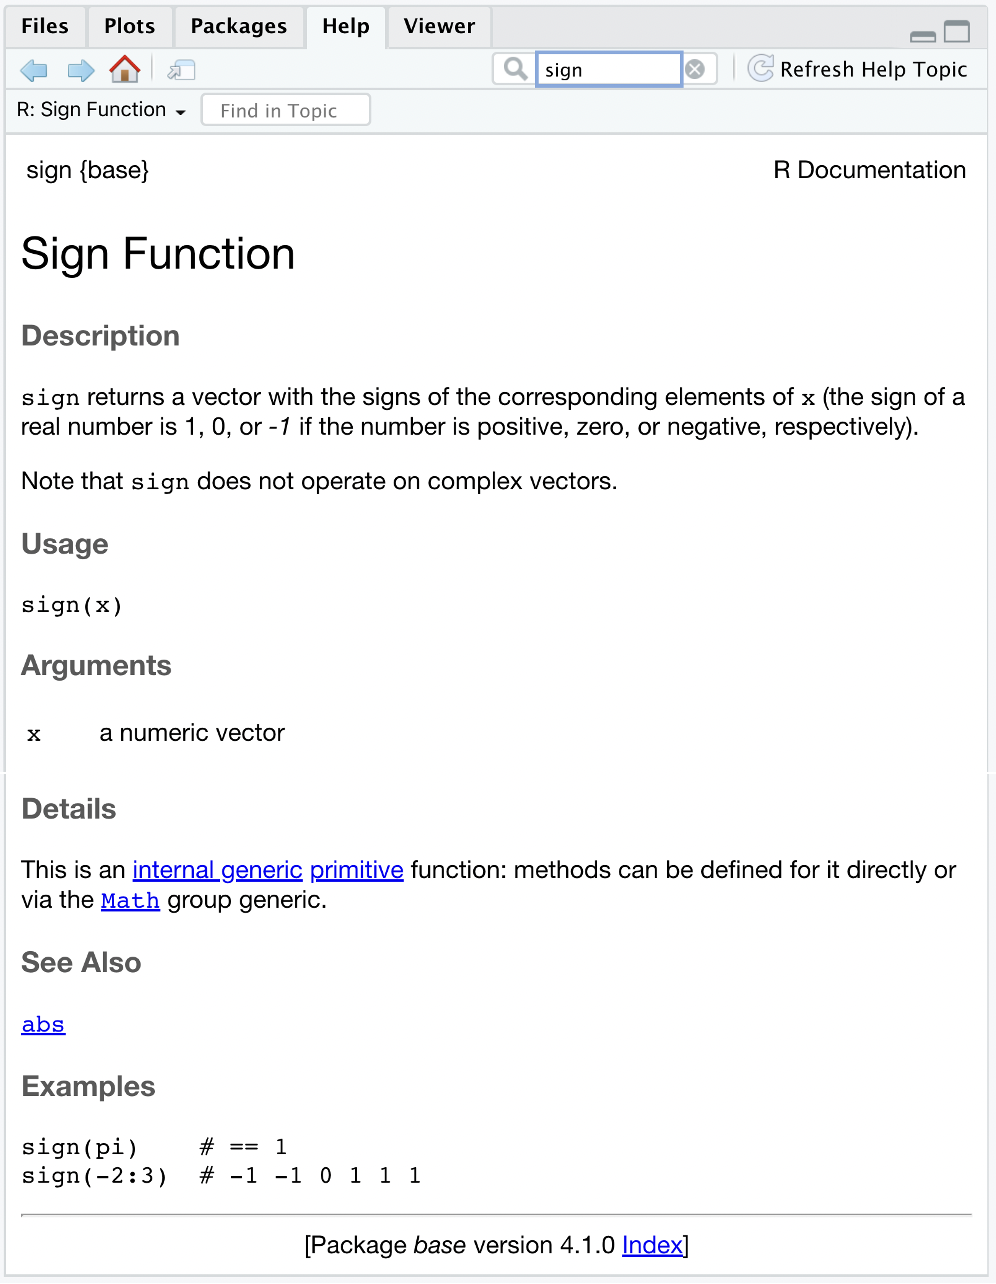
\includegraphics[width=0.7\linewidth]{pics/1d} 

}

\caption{Documentation for function}\label{fig:d}
\end{figure}

This documentation contains the following parts:

\begin{itemize}
\tightlist
\item
  \emph{Description}: A text-format introduction of the function of interest. The introduction describes the function's mechanism, the acceptable input and output types, and some notes of the function.
\item
  \emph{Usage}: The way the function looks like.
\item
  \emph{Arguments}: A detailed description of the input.
\item
  \emph{Details}: A detailed description of the function, including the background, some complicated usage, and special cases of the function.
\item
  \emph{See Also}: Some functions related or similar to this function.
\item
  \emph{Examples}: Sample codes and their corresponding answers. You can simply copy codes in the \emph{Examples} part and run them in the editor or in the console. Note that all words after \texttt{\#} are comments and will be ignored by R.
\end{itemize}

Here, from the documentation of the \texttt{sign()} function, you will know that the \texttt{sign()} function can return the signs of numbers, which means it will return 0 for zero, return 1 for positive numbers, and return -1 for negative numbers.

The documentation of different functions can contain different parts, we will give you the introduction of other functions in the following sections.

\hypertarget{approximation}{%
\subsection{Approximation}\label{approximation}}

Next, let's move on to the approximation in R. When computing \texttt{7\ /\ 3}, the answer is not a whole number as 7 is not divisible by 3. Approximation will come in handy under such circumstances. Let's take \texttt{7\ /\ 3} as the example.

\textbf{\emph{a. Get the integer part and the remainder}}

\begin{tabular}{l|l}
\hline
Code & Name\\
\hline
7\%/\%3 & integer division\\
\hline
7\%\%3 & modulus\\
\hline
\end{tabular}

We all know that 7 = 3 * \textbf{2} + \textbf{1}. So the \emph{integer division} will pick up the integer part, which is 2 here; and the \emph{modulus} will get the remainder, which is 1.

\textbf{\emph{b. Get the nearby integer}}

\begin{Shaded}
\begin{Highlighting}[]
\FunctionTok{floor}\NormalTok{(}\DecValTok{7} \SpecialCharTok{/} \DecValTok{3}\NormalTok{)   }
\CommentTok{\#\textgreater{} [1] 2}
\FunctionTok{ceiling}\NormalTok{(}\DecValTok{7} \SpecialCharTok{/} \DecValTok{3}\NormalTok{) }
\CommentTok{\#\textgreater{} [1] 3}
\end{Highlighting}
\end{Shaded}

Since \textbf{2} \textless= 7/3 \textless= \textbf{3}, you can use the \texttt{floor} function to find the \emph{largest integer} \textless= 7/3, which is 2; and the \texttt{ceiling} function gives the \emph{smallest integer} \textgreater= 7/3, which is 3.

\textbf{\emph{c.~Round to the nearest number}}

\begin{Shaded}
\begin{Highlighting}[]
\FunctionTok{round}\NormalTok{(}\DecValTok{7} \SpecialCharTok{/} \DecValTok{3}\NormalTok{)   }
\CommentTok{\#\textgreater{} [1] 2}
\FunctionTok{round}\NormalTok{(}\DecValTok{7} \SpecialCharTok{/} \DecValTok{3}\NormalTok{, }\AttributeTok{digits =} \DecValTok{3}\NormalTok{)}
\CommentTok{\#\textgreater{} [1] 2.333}
\end{Highlighting}
\end{Shaded}

The \texttt{round()} function follows the \textbf{rounding principle}. By default, you will get the nearest integer to \texttt{7\ /\ 3}, which is \texttt{2}. If you want to control the approximation accuracy, you can add a \texttt{digits} argument to specify how many digits you want after the decimal point. Here you will get \texttt{2.333} after adding \texttt{digits\ =\ 3}.

\hypertarget{power-logarithm}{%
\subsection{Power \& logarithm}\label{power-logarithm}}

You can also use R to do \emph{power} and \emph{logarithmic} operations.

Generally, you can use \texttt{\^{}} to do power operations. For example, \texttt{10\^{}5} will give us 10 to the power of 5. Here, 10 is the \emph{base} value, and 5 is the \emph{exponent}. The result is 100000, but it is shown as \texttt{1e+05} in R. That's because R uses the so-called \emph{scientific notation}.

\begin{infobox}{caution}
\textbf{scientific notation}: a common way to express numbers which are too large or too small to be conveniently written in decimal form. Generally, it expresses numbers in forms of \(m \times 10^n\) and R uses the \textbf{e notation}. Note that the \textbf{e notation} has nothing to do with the natural number \(e\). Let's see some examples,
\begin{align}
1 \times 10^5 &= \mbox{1e+05}\\
2 \times 10^4 &= \mbox{2e+04}\\
1.2 \times 10^{-3} &= \mbox{1.2e-03}
\end{align}

\end{infobox}

In mathematics, the \emph{logarithmic operations} are inverse to the power operations. If \textbf{\(b^y = x\)} and you only know \emph{\(b\)} and \emph{\(x\)}, you can do logarithmic operations to solve \emph{\(y\)} using the general form \textbf{\(y = \log(x, b)\)}, which is called the logarithm of \(x\) with base \(b\).

In R, logarithm functions with base value of 10, 2, or the natural number \(e\) have shortcuts \texttt{log10()}, \texttt{log2()}, and \texttt{log()}, respectively. Let's see an example of \texttt{log10()}, the logarithm function with base \emph{10}. Here, we have added a comment to help you have a better understanding of \texttt{log10()}.

\begin{Shaded}
\begin{Highlighting}[]
\DecValTok{10}\SpecialCharTok{\^{}}\DecValTok{6} 
\CommentTok{\#\textgreater{} [1] 1e+06}
\FunctionTok{log10}\NormalTok{(}\FloatTok{1e6}\NormalTok{) }\CommentTok{\#log10(x) = log(x, 10)}
\CommentTok{\#\textgreater{} [1] 6}
\end{Highlighting}
\end{Shaded}

Next, let's see \texttt{log2()}, the logarithm function with base \emph{2}. There is also a comment for \texttt{log2()} here.

\begin{Shaded}
\begin{Highlighting}[]
\DecValTok{2}\SpecialCharTok{\^{}}\DecValTok{10}
\CommentTok{\#\textgreater{} [1] 1024}
\FunctionTok{log2}\NormalTok{(}\DecValTok{1024}\NormalTok{)  }\CommentTok{\#log2(x) = log(x, 2)}
\CommentTok{\#\textgreater{} [1] 10}
\end{Highlighting}
\end{Shaded}

Before moving on to the natural logarithm, note that the natural number \(e\) needs to be written as \texttt{exp(1)} in R. When you want to do power operations on \(e\), you can simply change the argument in the function \texttt{exp()}. For example, \texttt{exp(3)} is \(e\) to the power of 3. Here, \texttt{log()} without specifying the \texttt{base} argument represents the logarithm function with base \(e\). You can see the general form of \texttt{log()} in the comment.

\begin{Shaded}
\begin{Highlighting}[]
\FunctionTok{exp}\NormalTok{(}\DecValTok{1}\NormalTok{)      }
\CommentTok{\#\textgreater{} [1] 2.718282}
\FunctionTok{exp}\NormalTok{(}\DecValTok{3}\NormalTok{)}
\CommentTok{\#\textgreater{} [1] 20.08554}
\FunctionTok{log}\NormalTok{(}\FunctionTok{exp}\NormalTok{(}\DecValTok{3}\NormalTok{))  }\CommentTok{\#log(x) = log(x, exp(1))}
\CommentTok{\#\textgreater{} [1] 3}
\end{Highlighting}
\end{Shaded}

\hypertarget{trigonometric-function}{%
\subsection{Trigonometric function}\label{trigonometric-function}}

R also provides the common trigonometric functions.

\begin{Shaded}
\begin{Highlighting}[]
\FunctionTok{cos}\NormalTok{(pi)}
\CommentTok{\#\textgreater{} [1] {-}1}
\FunctionTok{acos}\NormalTok{(}\SpecialCharTok{{-}}\DecValTok{1}\NormalTok{)}
\CommentTok{\#\textgreater{} [1] 3.141593}
\end{Highlighting}
\end{Shaded}

Here, \texttt{acos()} is the inverse function of \texttt{cos()}. If we set \(cos(a) = b\), then we will get \(acos(b) = a\).

\begin{Shaded}
\begin{Highlighting}[]
\FunctionTok{sin}\NormalTok{(pi}\SpecialCharTok{/}\DecValTok{2}\NormalTok{)}
\CommentTok{\#\textgreater{} [1] 1}
\FunctionTok{asin}\NormalTok{(}\DecValTok{1}\NormalTok{)}
\CommentTok{\#\textgreater{} [1] 1.570796}
\end{Highlighting}
\end{Shaded}

Similarly, \texttt{asin()} is the inverse function of \texttt{sin()}. If we set \(sin(a) = b\), then we will get \(asin(b) = a\).

\begin{Shaded}
\begin{Highlighting}[]
\FunctionTok{tan}\NormalTok{(pi}\SpecialCharTok{/}\DecValTok{4}\NormalTok{)}
\CommentTok{\#\textgreater{} [1] 1}
\FunctionTok{atan}\NormalTok{(}\DecValTok{1}\NormalTok{)}
\CommentTok{\#\textgreater{} [1] 0.7853982}
\end{Highlighting}
\end{Shaded}

Also, \texttt{atan()} is the inverse function of \texttt{tan()}. If we set \(tan(a) = b\), then we will get \(atan(b) = a\).

\hypertarget{exercises-1}{%
\subsection{Exercises}\label{exercises-1}}

\begin{enumerate}
\def\labelenumi{\arabic{enumi}.}
\item
  Write R code to compute \(\sqrt{5 \times 5}\).
\item
  Write R code to get help on the function \texttt{floor}.
\item
  Write R code to compute the square of \(\pi\) and round it to 4 digits after the decimal point.
\item
  Write R code to compute the logarithm of 1 billion with base 1000.
\item
  Write R code to verify \(sin^2(x) + cos^2(x) = 1\), for \(x = 724\).
\end{enumerate}

\hypertarget{Object-Assignment}{%
\section{Object Assignment}\label{Object-Assignment}}

In the last section, you have seen the power of R as a fancy calculator. However, in order to do more complicated and interesting tasks, it is super helpful to store intermediate results for future use.

Let's take a look at a concrete example. Say if you want to do the following three calculations, all involving \texttt{exp(3)\ /\ log(20,3)\ *\ 7}.

\begin{Shaded}
\begin{Highlighting}[]
\NormalTok{(}\FunctionTok{exp}\NormalTok{(}\DecValTok{3}\NormalTok{) }\SpecialCharTok{/} \FunctionTok{log}\NormalTok{(}\DecValTok{20}\NormalTok{,}\DecValTok{3}\NormalTok{) }\SpecialCharTok{*} \DecValTok{7}\NormalTok{) }\SpecialCharTok{+} \DecValTok{3} \CommentTok{\#addition}
\NormalTok{(}\FunctionTok{exp}\NormalTok{(}\DecValTok{3}\NormalTok{) }\SpecialCharTok{/} \FunctionTok{log}\NormalTok{(}\DecValTok{20}\NormalTok{,}\DecValTok{3}\NormalTok{) }\SpecialCharTok{*} \DecValTok{7}\NormalTok{) }\SpecialCharTok{{-}} \DecValTok{3} \CommentTok{\#subtraction}
\NormalTok{(}\FunctionTok{exp}\NormalTok{(}\DecValTok{3}\NormalTok{) }\SpecialCharTok{/} \FunctionTok{log}\NormalTok{(}\DecValTok{20}\NormalTok{,}\DecValTok{3}\NormalTok{) }\SpecialCharTok{*} \DecValTok{7}\NormalTok{) }\SpecialCharTok{/} \DecValTok{3} \CommentTok{\#division}
\end{Highlighting}
\end{Shaded}

Using R as a fancy calculator (Section \ref{Calculator}), you need to type the expression \texttt{exp(3)\ /\ log(20,3)\ *\ 7} three times, which is a bit cumbersome. In this section, you will learn how to do \textbf{object assignment}, which can avoid the need for typing the same expression more than once.

\hypertarget{what-is-an-r-object}{%
\subsection{What is an R Object?}\label{what-is-an-r-object}}

Before we get into the details, let's first introduce \textbf{object}, which is perhaps the most fundamental thing in R. In principle, \textbf{everything that exists in R is an object}. For example, the number \texttt{5} is an object, the expression \texttt{1\ +\ 2} is an object, and the expression \texttt{exp(3)\ /\ log(20,3)\ *\ 7} is also an object.

If you run \texttt{5}, you will get one element of value 5 from the output. Similarly, if you run \texttt{1\ +\ 2}, you will get one element of value 3 from the output. You can try to run \texttt{exp(3)\ /\ log(20,3)\ *\ 7} by yourself. In these three examples, you can see that there is only one \textbf{element} in each object.

However, an object can contain more than one elements, and each element has its own \textbf{value}, which is possibly different from that of another element. Naturally, different objects can contain different values.

\hypertarget{assignment}{%
\subsection{\texorpdfstring{Assignment Operation with \texttt{\textless{}-}}{Assignment Operation with \textless-}}\label{assignment}}

With the importance of objects in mind, let's learn how to do \textbf{object assignments} in R. To do object assignments, you need to assign \textbf{value(s)} to a \textbf{name} via the \textbf{assignment operator}, which will create a new object with the name you specified. Once the object assignment operation is done, you can simply use the name in subsequent calculations without redundancy. Let's start with a simple example,

\begin{Shaded}
\begin{Highlighting}[]
\NormalTok{x\_num }\OtherTok{\textless{}{-}} \DecValTok{5}
\end{Highlighting}
\end{Shaded}

The assignment operation has three components. From left to right,

\begin{itemize}
\tightlist
\item
  the first component \texttt{x\_num} is the \textbf{object name} of a new object, which has certain naming rules that will be discussed shortly in Section \ref{Naming}.
\item
  The second component is the \textbf{assignment operator} \texttt{\textless{}-}, which is a combination of the less than sign \texttt{\textless{}} immediately followed by the minus sign \texttt{-}, with \textbf{no space} in between.
\item
  The final component is the object name's assigned \textbf{value(s)}, which is 5 here.
\end{itemize}

\begin{infobox}{caution}
There is no space between \texttt{\textless{}} and \texttt{-} in the assignment operator \texttt{\textless{}-}. Note that although \texttt{=} may also appear to be working as the assignment operator, it is not recommended as \texttt{=} is usually reserved for specifying the value(s) of arguments in a function call, which will be introduced in Section \ref{vector-patterns}.

\end{infobox}

After running the code above, you will see no output in the console, unlike the situation when we ran \texttt{1\ +\ 2} which gives us the answer \texttt{3} (as shown in Figure \ref{fig:noa}). You may be wondering, did we successfully make our first assignment operation?

\begin{figure}

{\centering 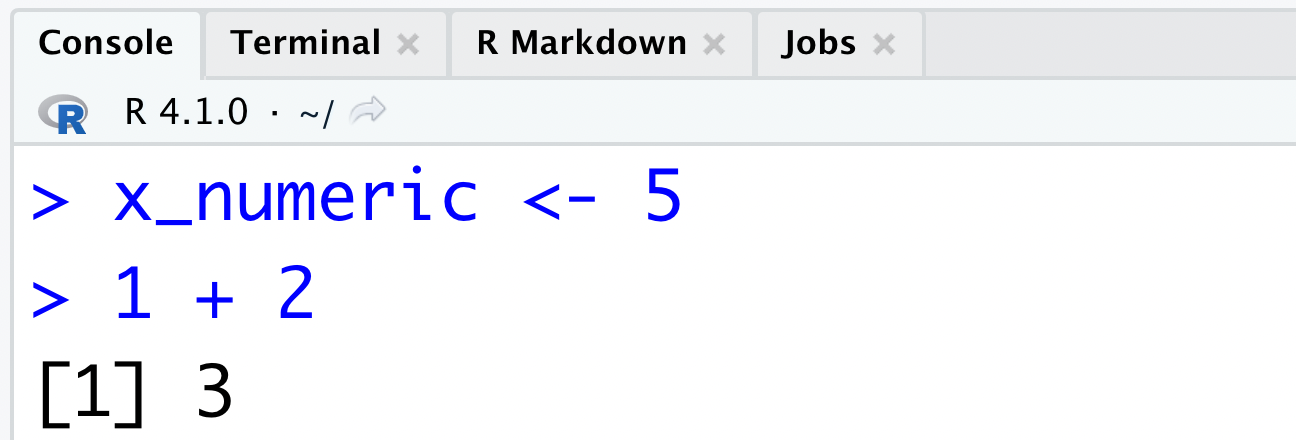
\includegraphics[width=0.7\linewidth]{pics/2noa} 

}

\caption{No output}\label{fig:noa}
\end{figure}

To verify it, you can run the code with just the object name to check its value. (For all named objects, you can get their value(s) by running codes with just their names.)

\begin{Shaded}
\begin{Highlighting}[]
\NormalTok{x\_num}
\CommentTok{\#\textgreater{} [1] 5}
\end{Highlighting}
\end{Shaded}

Great! The output is 5, indicating that you have successfully assigned the value 5 to the name x\_num, and you have created a new object \texttt{x\_num}. You can use \texttt{x\_num} instead of \texttt{5} to do the subsequent calculations because \texttt{x\_num} and \texttt{5} have the same value.

Note that R object names are \textbf{case-sensitive}. For example, you have defined \texttt{x\_num}, but if you type \texttt{X\_num}, the console will return an error message as follow.

\begin{Shaded}
\begin{Highlighting}[]
\NormalTok{X\_num}
\CommentTok{\#\textgreater{} Error in eval(expr, envir, enclos): object \textquotesingle{}X\_num\textquotesingle{} not found}
\end{Highlighting}
\end{Shaded}

In addition, you can assign \textbf{value(s)} of an expression to a name. Let's try to simplify the three expressions we showed at the beginning of this section. It is easy to observe that the three expressions share a common term \texttt{exp(3)\ /\ log(20,3)\ *\ 7}. Let's assign the common term to a name.

\begin{Shaded}
\begin{Highlighting}[]
\NormalTok{y\_num }\OtherTok{\textless{}{-}} \FunctionTok{exp}\NormalTok{(}\DecValTok{3}\NormalTok{) }\SpecialCharTok{/} \FunctionTok{log}\NormalTok{(}\DecValTok{20}\NormalTok{,}\DecValTok{3}\NormalTok{) }\SpecialCharTok{*} \DecValTok{7}
\NormalTok{y\_num}
\CommentTok{\#\textgreater{} [1] 51.56119}
\end{Highlighting}
\end{Shaded}

Now you have successfully created an object \texttt{y\_num} with value 51.561191. Using the named object \texttt{y\_num}, you can simplify the three calculations as follows.

\begin{Shaded}
\begin{Highlighting}[]
\NormalTok{y\_num }\SpecialCharTok{+} \DecValTok{3}
\NormalTok{y\_num }\SpecialCharTok{{-}} \DecValTok{3}
\NormalTok{y\_num }\SpecialCharTok{/} \DecValTok{3}
\end{Highlighting}
\end{Shaded}

\begin{infobox}{caution}
Note that in the object assignment process, it is not the expression itself but rather the value(s) of the expression, that is assigned to a name. So you will not get the expression \texttt{exp(3)\ /\ log(20,3)\ *\ 7} by running \texttt{y\_num}.

\end{infobox}

You can also try the following examples by yourself.

\begin{Shaded}
\begin{Highlighting}[]
\NormalTok{z\_num1 }\OtherTok{\textless{}{-}} \FunctionTok{floor}\NormalTok{(}\DecValTok{7} \SpecialCharTok{/} \DecValTok{3}\NormalTok{) }
\NormalTok{z\_num1}
\NormalTok{z\_num2 }\OtherTok{\textless{}{-}} \DecValTok{7}\SpecialCharTok{\%/\%}\DecValTok{3}
\NormalTok{z\_num2}
\end{Highlighting}
\end{Shaded}

Clearly, using the object assignment, you can greatly simplify the code and avoid redundancy.

\hypertarget{Naming}{%
\subsection{Object naming rule}\label{Naming}}

As you now see, the assignment operation in R is very straightforward. In general, R is very flexible in the name you can give to an object. However, there are three important rules you need to follow.

\textbf{\emph{a. Must start with a letter or . (period)}}

In addition, if starting with period, the second character can't be a number.

\textbf{\emph{b. Can only contain letters, numbers, \texttt{\_} (underscore), and \texttt{.} (period)}}

One recommended naming style is to use lowercase letters and numbers, and use underscore to separate words within a name. So you can use relatively longer names that is more readable. For example, \texttt{this\_is\_name\_6} and \texttt{super\_rich\_88} are great names.

\textbf{\emph{c.~Can not use special keywords as names.}}

For example, \texttt{TRUE\ \textless{}-\ 12} is not permitted as \texttt{TRUE} is a special keyword in R. You can see from the following that this assignment operation leads to an error message.

\begin{Shaded}
\begin{Highlighting}[]
\ConstantTok{TRUE} \OtherTok{\textless{}{-}} \DecValTok{12}
\CommentTok{\#\textgreater{} Error in TRUE \textless{}{-} 12: invalid (do\_set) left{-}hand side to assignment}
\end{Highlighting}
\end{Shaded}

Some commonly used reserved keywords that cannot be used as names are listed as below.

\begin{tabular}{l|l}
\hline
TRUE & else\\
\hline
FALSE & for\\
\hline
NA & while\\
\hline
Inf & break\\
\hline
NaN & next\\
\hline
function & repeat\\
\hline
if & return\\
\hline
\end{tabular}

To get a complete list of reserved words, you can run the following code.

\begin{Shaded}
\begin{Highlighting}[]
\NormalTok{?Reserved}
\end{Highlighting}
\end{Shaded}

\hypertarget{review-objects-in-environment}{%
\subsection{Review objects in environment}\label{review-objects-in-environment}}

At this point, we've introduced the rules of creating objects in R. Now, you can also confirm the success of object assignments by inspecting the \textbf{Environment}, located in the top right panel (\textbf{panel3 in Figure \ref{fig:four} in Section \ref{Installation}}).

If you exercised previous examples, you can find the newly assigned objects \texttt{x\_num} and \texttt{y\_num} (possibly also \texttt{z\_num1} and \texttt{z\_num2}) in your \emph{Environment} Viewer. You may also notice that the name \texttt{TRUE}, which we tried but failed to assign the value 12 to, doesn't appear in the \emph{Environment} (as shown in Figure \ref{fig:en}). You can check all the \textbf{named objects} and their values in this area.

\begin{figure}

{\centering 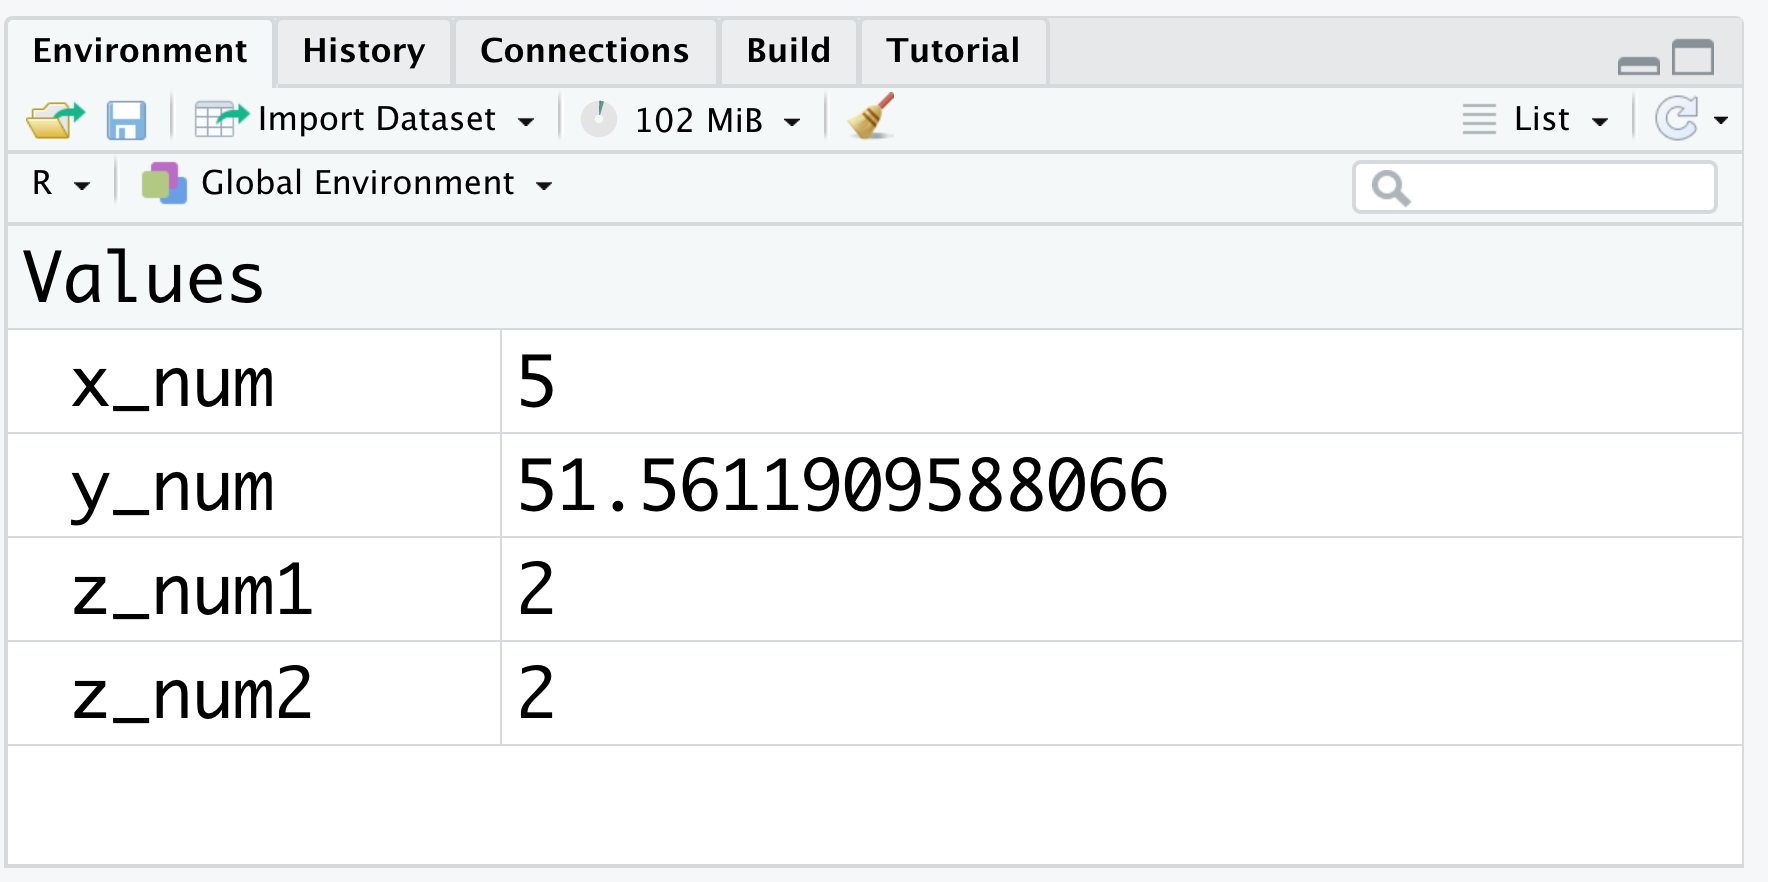
\includegraphics[width=0.7\linewidth]{pics/1en} 

}

\caption{The environment (I)}\label{fig:en}
\end{figure}

From the picture above, you can see that the value of \texttt{x\_num} is 5. In this case, let's try to assign the new value 6 to \texttt{x\_num} and see what will happen next.

\begin{Shaded}
\begin{Highlighting}[]
\NormalTok{x\_num }\OtherTok{\textless{}{-}} \DecValTok{6}
\NormalTok{x\_num  }\CommentTok{\#check its value}
\CommentTok{\#\textgreater{} [1] 6}
\end{Highlighting}
\end{Shaded}

Now you can see that the value of \texttt{x\_num} has changed from 5 to 6. Generally, when assigning a new value to an object, R will update the object's value, and the previous value will no longer be stored. You can verify the result by inspecting the Environment tab, where only the new value of the object will be displayed.

\begin{figure}

{\centering 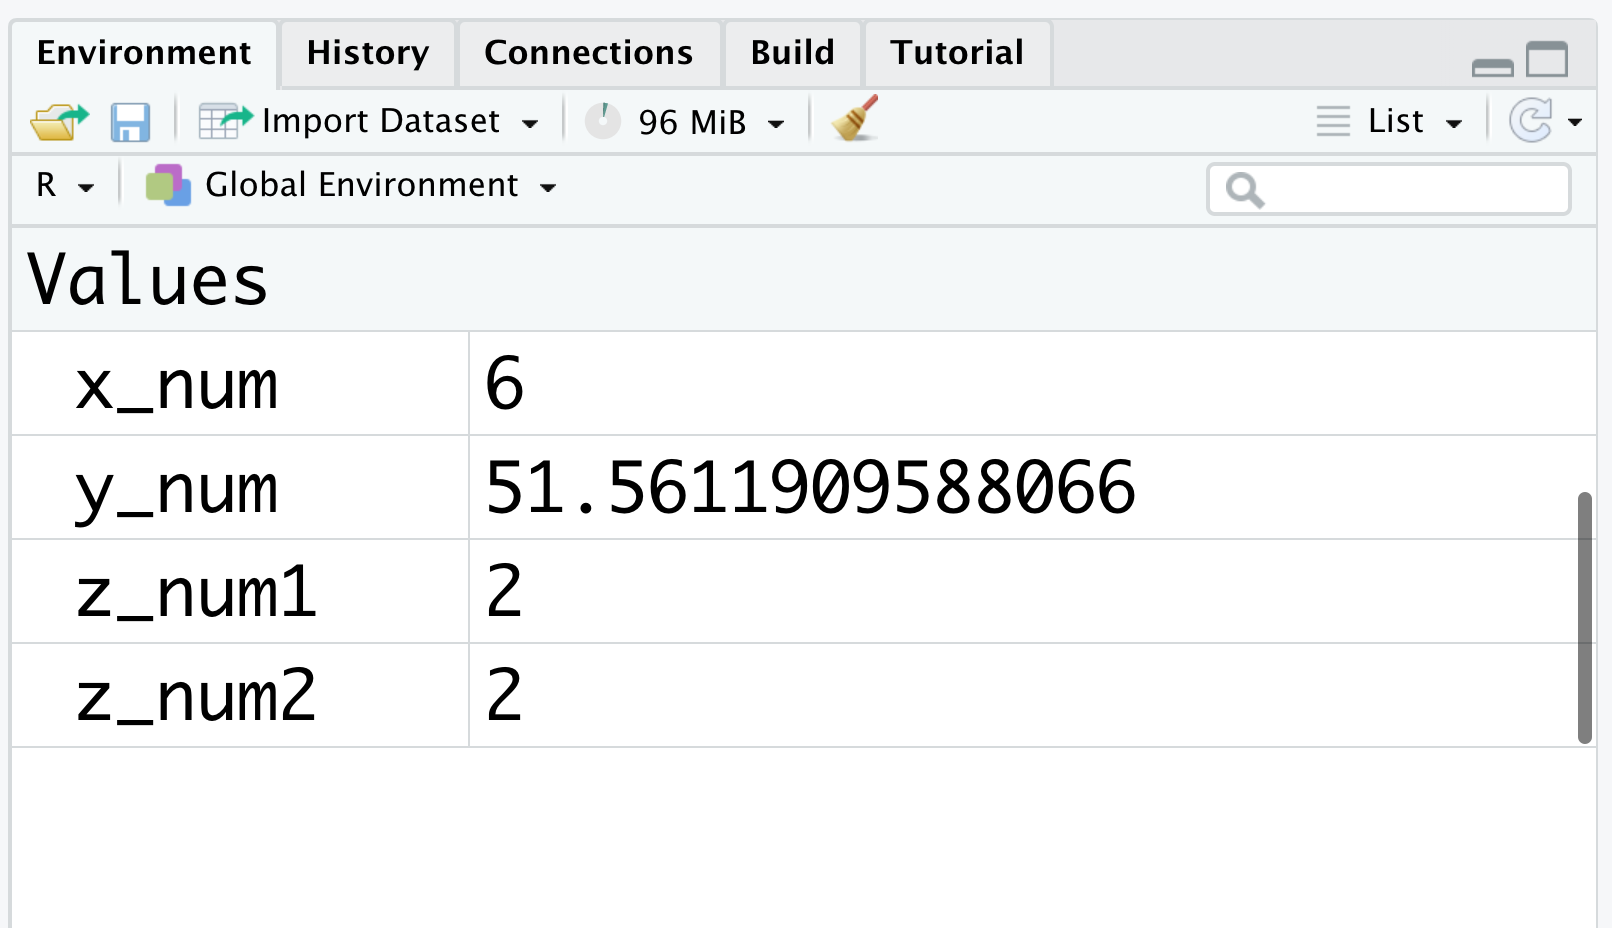
\includegraphics[width=0.7\linewidth]{pics/1en2} 

}

\caption{The environment (II)}\label{fig:en2}
\end{figure}

So it is helpful to monitor the environment from time to time to make sure everything looks fine. Notice that objects without names will \emph{not} be shown in the environment.

You can also see the list of all the named objects (just names without values) using the built-in R function \texttt{ls()}.

\begin{Shaded}
\begin{Highlighting}[]
\FunctionTok{ls}\NormalTok{()}
\CommentTok{\#\textgreater{} [1] "key\_mat" "Keys"    "x\_num"   "y\_num"}
\end{Highlighting}
\end{Shaded}

All the objects shown in the environment or on the list are stored in the memory, so they are available for us in subsequent codes. It is a good habit to do object assignments if you want to retrieve their values at a later time.

\hypertarget{object-types}{%
\subsection{Object types}\label{object-types}}

So far in this section, you have learned how to do object assignments. The values you assigned are all numbers, i.e.~of numeric type. Actually, an object may contain more than one values. Also, an object may contain values other than the numeric type, such like character and logical ones. Depending on the \textbf{composition of values}, the object belongs to one particular type.

\begin{tabular}{l|l}
\hline
Type & Section\\
\hline
Atomic Vector & \textbackslash{}@ref(r-objects)\\
\hline
Matrix & \textbackslash{}@ref(matrix)\\
\hline
Array & \textbackslash{}@ref(array)\\
\hline
Data Frame & \textbackslash{}@ref(dataframe)\\
\hline
Tibble & \textbackslash{}@ref(tibble)\\
\hline
List & \textbackslash{}@ref(list)\\
\hline
\end{tabular}

We will focus on atomic vectors in Chapter \ref{r-objects} and discuss other object types in Chapter \ref{r-objects-other-types}.

While some of the object types look more intuitive than others, you have nothing to worry about since we have the next two chapters devoted to the details of R objects. Objects are the building blocks of R programming and it will be time well spent mastering every object type.

\hypertarget{exercises-2}{%
\subsection{Exercises}\label{exercises-2}}

\begin{enumerate}
\def\labelenumi{\arabic{enumi}.}
\item
  Write the R code to assign the value 20 to the name \texttt{num\_1}.
\item
  Which of the following is a valid object name in R?
\end{enumerate}

\begin{itemize}
\tightlist
\item
  \texttt{2.True}
\item
  \texttt{else}
\item
  \texttt{I\_am\_not\_a\_valid\_name}
\item
  \texttt{I\_am\_a\_Pretty\#\_name}
\end{itemize}

\begin{enumerate}
\def\labelenumi{\arabic{enumi}.}
\setcounter{enumi}{2}
\tightlist
\item
  Write the R code to get the list of all objects in the environment.
\end{enumerate}

\hypertarget{r-objects}{%
\chapter{R Objects (I): Atomic Vectors}\label{r-objects}}

In this chapter, we focus on the most fundamental R object type: \textbf{atomic vectors}. We will introduce different types of atomic vectors, creating vectors with patterns, applying different functions and operations on vectors, comparing and extracting vectors. We will also discuss data and times, factors, and how R represents unexpected results.

\hypertarget{intro-num-vector}{%
\section{Introduction to Numeric Vectors}\label{intro-num-vector}}

We will start off this chapter by learning \textbf{numeric vectors}. Numeric vectors are perhaps the most commonly used member of the \textbf{atomic vector} family, where all elements are of the same type.

\hypertarget{create-numeric-vector}{%
\subsection{Creation and class}\label{create-numeric-vector}}

A \textbf{numeric vector} is an atomic vector containing only numbers. For example, \texttt{6} is a numeric vector with one element of value 6.

By assigning the value 6 to the name x1, you can create a new numeric vector \texttt{x1} with value 6. As a result, you can refer to \texttt{x1} in subsequent calculations. For any vector, you can use the \texttt{length()} function to check the number of elements it contains.

\begin{Shaded}
\begin{Highlighting}[]
\DecValTok{6}                         \CommentTok{\#a numeric vector}
\CommentTok{\#\textgreater{} [1] 6}
\NormalTok{x1 }\OtherTok{\textless{}{-}} \DecValTok{6}                   \CommentTok{\#x1 is also a numeric vector}
\NormalTok{x1                        }\CommentTok{\#check the value of x1}
\CommentTok{\#\textgreater{} [1] 6}
\FunctionTok{length}\NormalTok{(}\DecValTok{6}\NormalTok{)                 }\CommentTok{\#length of 6}
\CommentTok{\#\textgreater{} [1] 1}
\FunctionTok{length}\NormalTok{(x1)                }\CommentTok{\#length of x1}
\CommentTok{\#\textgreater{} [1] 1}
\end{Highlighting}
\end{Shaded}

Given the output, you can see that \texttt{6} is a numeric vector with length 1 and you have successfully created the numeric vector \texttt{x1} of length 1.

Moving on, you may wonder, can a numeric vector contain more than one value? The answer is a big YES! In R, you can use the \texttt{c()} function (\texttt{c} is short for combine) to store several elements into one single numeric vector.

\begin{Shaded}
\begin{Highlighting}[]
\FunctionTok{c}\NormalTok{(}\DecValTok{1}\NormalTok{, }\DecValTok{3}\NormalTok{, }\DecValTok{3}\NormalTok{, }\DecValTok{5}\NormalTok{, }\DecValTok{5}\NormalTok{)          }\CommentTok{\#use c() to combine elements into a numeric vector of length 5}
\CommentTok{\#\textgreater{} [1] 1 3 3 5 5}
\NormalTok{y1 }\OtherTok{\textless{}{-}} \FunctionTok{c}\NormalTok{(}\DecValTok{1}\NormalTok{, }\DecValTok{3}\NormalTok{, }\DecValTok{3}\NormalTok{, }\DecValTok{5}\NormalTok{, }\DecValTok{5}\NormalTok{)    }\CommentTok{\#y1 is a numeric vector of length 5}
\NormalTok{y1                        }\CommentTok{\#check the value of y1}
\CommentTok{\#\textgreater{} [1] 1 3 3 5 5}
\FunctionTok{length}\NormalTok{(y1)                }\CommentTok{\#length of y1}
\CommentTok{\#\textgreater{} [1] 5}
\end{Highlighting}
\end{Shaded}

In this example, firstly you have created a length-5 object using the \texttt{c()} function with arguments being the five elements separated by \textbf{comma}. Since all elements are numbers, this object is still a numeric vector. Then after assigning the values to the name y1, you will get a new numeric vector \texttt{y1} with 5 elements. Among the five elements, although some of them have the same value, R still recognizes and stores them separately. This is the reason why the length of \texttt{y1} is 5 instead of 3.

Similar to \texttt{x1}, you can verify the contents of \texttt{y1} and check the length of it via the \texttt{length()} function.

\begin{infobox}{caution}

When you assign several values to a name, the order of the values will not change after assignment. If you create two numeric vectors containing the same numbers but in different orders, the two vectors will be two different ones maintaining the specified orders. For example,

\begin{Shaded}
\begin{Highlighting}[]
\NormalTok{y2 }\OtherTok{\textless{}{-}} \FunctionTok{c}\NormalTok{(}\DecValTok{1}\NormalTok{, }\DecValTok{3}\NormalTok{, }\DecValTok{5}\NormalTok{, }\DecValTok{7}\NormalTok{, }\DecValTok{9}\NormalTok{)    }
\NormalTok{y2                        }
\CommentTok{\#\textgreater{} [1] 1 3 5 7 9}
\NormalTok{y3 }\OtherTok{\textless{}{-}} \FunctionTok{c}\NormalTok{(}\DecValTok{9}\NormalTok{, }\DecValTok{7}\NormalTok{, }\DecValTok{5}\NormalTok{, }\DecValTok{3}\NormalTok{, }\DecValTok{1}\NormalTok{)    }
\NormalTok{y3}
\CommentTok{\#\textgreater{} [1] 9 7 5 3 1}
\end{Highlighting}
\end{Shaded}

\end{infobox}

In addition to using numbers inside the \texttt{c()} function, you can also use numeric vectors as the arguments to create a longer vector. The new, longer vector will combine the input numeric vectors in the given order.

\begin{Shaded}
\begin{Highlighting}[]
\FunctionTok{c}\NormalTok{(x1, y1)          }\CommentTok{\#use c() to combine several numeric vectors into one numeric vector}
\CommentTok{\#\textgreater{} [1] 6 1 3 3 5 5}
\NormalTok{z1 }\OtherTok{\textless{}{-}} \FunctionTok{c}\NormalTok{(x1, y1)}
\NormalTok{z1}
\CommentTok{\#\textgreater{} [1] 6 1 3 3 5 5}
\FunctionTok{length}\NormalTok{(z1)}
\CommentTok{\#\textgreater{} [1] 6}
\end{Highlighting}
\end{Shaded}

Since \texttt{x1} contains 1 numeric value and \texttt{y1} contains 5 numeric values, \texttt{z1} is a numeric vector of length 6 after combination.

For any vector, you can use the function \texttt{class()} to check its \textbf{class}. A class can be thought of as a ``type,'' providing a description about the vector and determining what functions can be applied to it.

\begin{Shaded}
\begin{Highlighting}[]
\FunctionTok{class}\NormalTok{(x1)}
\CommentTok{\#\textgreater{} [1] "numeric"}
\FunctionTok{class}\NormalTok{(y1)}
\CommentTok{\#\textgreater{} [1] "numeric"}
\FunctionTok{class}\NormalTok{(z1)}
\CommentTok{\#\textgreater{} [1] "numeric"}
\end{Highlighting}
\end{Shaded}

From the results, you can see that \texttt{x1}, \texttt{y1}, and \texttt{z1} are all numeric, which is the reason why they are called \emph{numeric vectors}.

As introduced in Section \ref{Object-Assignment}, you can check the named objects via the environment panel as shown in Figure \ref{fig:en11}.

\begin{figure}

{\centering 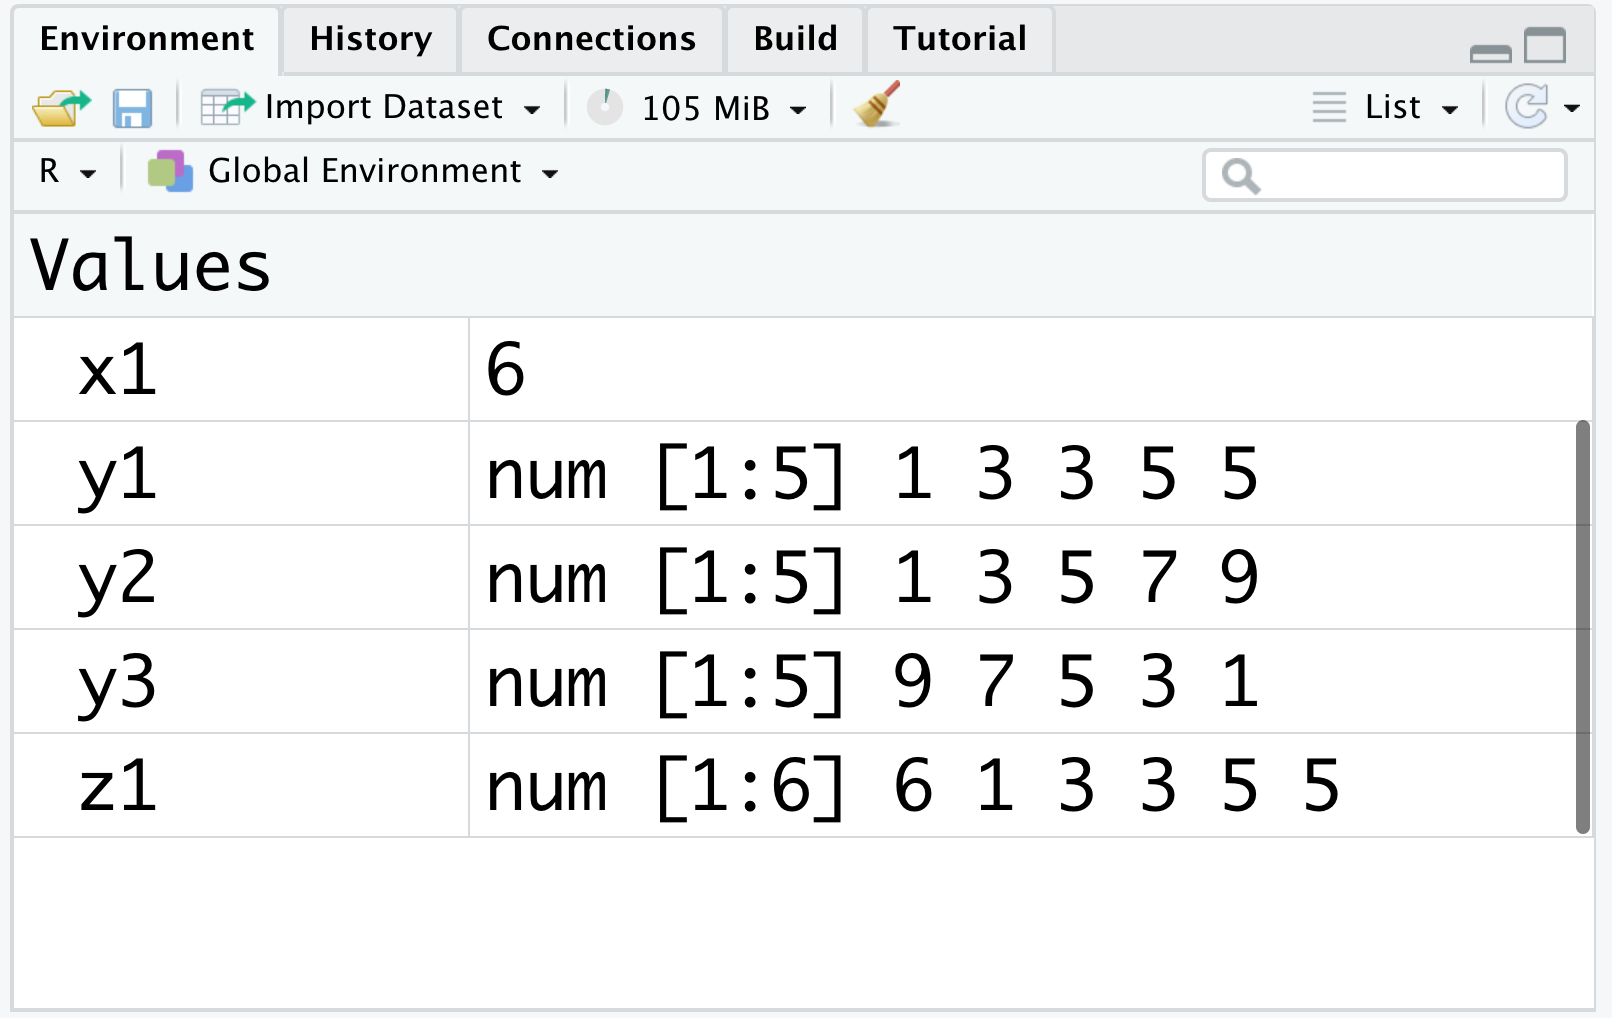
\includegraphics[width=0.7\linewidth]{pics/2en1} 

}

\caption{The environment (I)}\label{fig:en11}
\end{figure}

We can see that the environment panel has two columns, with the first column showing the list of object names and the second column showing the corresponding information for each object. The information includes the vector type (here \emph{num} is short for numeric), the vector length, and the value(s) of the vector. Note that if the vector is of length 1 (for example \texttt{x1}), the environment will not show the type or the length.

In the last section, we have introduced how to change the value of an object by reassigning it. Similarly, you can also assign a new value, or new values, to \texttt{x1}. Notice that the values you are going to assign can have different length with the previous values. Let's see an example,

\begin{Shaded}
\begin{Highlighting}[]
\NormalTok{z1 }\OtherTok{\textless{}{-}} \FunctionTok{c}\NormalTok{(}\DecValTok{6}\NormalTok{, }\DecValTok{1}\NormalTok{, }\DecValTok{3}\NormalTok{)}
\NormalTok{z1   }\CommentTok{\#check the value of z1}
\CommentTok{\#\textgreater{} [1] 6 1 3}
\end{Highlighting}
\end{Shaded}

Now, you can see that \texttt{z1} contains 3 numeric values, so \texttt{z1} is a numeric vector of length 3.

As expected, you can also view the newly assigned values of \texttt{z1} in the environment panel, as shown in Figure \ref{fig:en12}.

\begin{figure}

{\centering 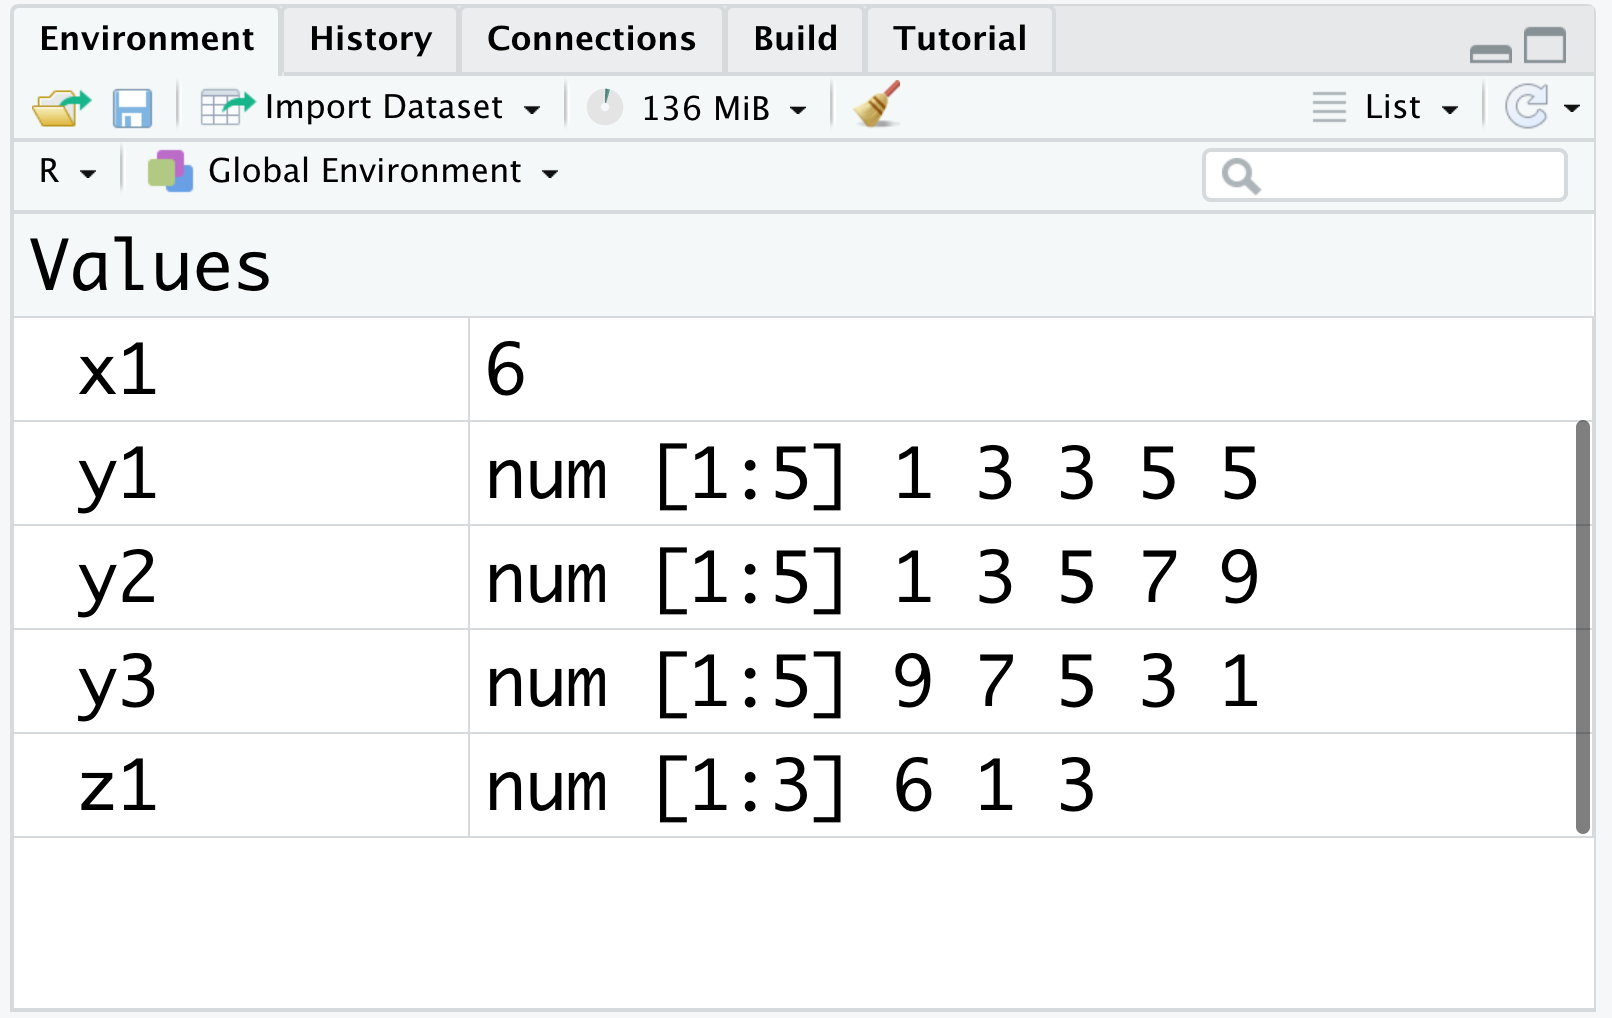
\includegraphics[width=0.7\linewidth]{pics/2en2} 

}

\caption{The environment (II)}\label{fig:en12}
\end{figure}

Finally, you can use the \texttt{vector(mode,\ length)} function to create a vector of certain \texttt{mode} and \texttt{length}.

\begin{Shaded}
\begin{Highlighting}[]
\FunctionTok{vector}\NormalTok{(}\StringTok{"numeric"}\NormalTok{, }\DecValTok{4}\NormalTok{)}
\end{Highlighting}
\end{Shaded}

\hypertarget{operation-recycling}{%
\subsection{Operations and recycling rule}\label{operation-recycling}}

Since numeric vectors are purely made of numbers, you can do \textbf{arithmetic operations} between them, just like the fancy calculator in Section \ref{Calculator}. If two or more vectors are of the \textbf{same length}, the operation is done \textbf{element-wisely}. In other words, R will perform the operation between elements in the same index of different vectors. First, let's create another vector \texttt{x2} of length 1 and compute the sum of \texttt{x1} and \texttt{x2}. Also recall that we've previously created a length-1 numeric vector \texttt{x1} with value 6.

\begin{Shaded}
\begin{Highlighting}[]
\NormalTok{x1}
\CommentTok{\#\textgreater{} [1] 6}
\NormalTok{x2 }\OtherTok{\textless{}{-}} \DecValTok{3}
\NormalTok{x1 }\SpecialCharTok{+}\NormalTok{ x2}
\CommentTok{\#\textgreater{} [1] 9}
\end{Highlighting}
\end{Shaded}

Then obviously you will get 9! If you assign this operation to a name, you will create a new numeric vector with the \emph{result} of the operation as the value.

\begin{Shaded}
\begin{Highlighting}[]
\NormalTok{s1 }\OtherTok{\textless{}{-}}\NormalTok{ x1 }\SpecialCharTok{+}\NormalTok{ x2}
\NormalTok{s1 }
\CommentTok{\#\textgreater{} [1] 9}
\end{Highlighting}
\end{Shaded}

Here, \texttt{s1} is a length-1 numeric vector with value 9.

Similarly, you can create another vector \texttt{y2} of the same length as vector \texttt{y1}. Then, you can do operations between \texttt{y1} and \texttt{y2}.

\begin{Shaded}
\begin{Highlighting}[]
\NormalTok{y1}
\CommentTok{\#\textgreater{} [1] 1 3 3 5 5}
\NormalTok{y2 }\OtherTok{\textless{}{-}} \FunctionTok{c}\NormalTok{(}\DecValTok{2}\NormalTok{, }\DecValTok{4}\NormalTok{, }\DecValTok{1}\NormalTok{, }\DecValTok{3}\NormalTok{, }\DecValTok{2}\NormalTok{)}
\NormalTok{y1 }\SpecialCharTok{*}\NormalTok{ y2}
\CommentTok{\#\textgreater{} [1]  2 12  3 15 10}
\end{Highlighting}
\end{Shaded}

The result is yet another length-5 vector. To check the calculation was indeed done element-wisely, you can verify that the value of the first element is \(1 * 2 = 2\), and value of the second element is \(3 * 4 = 12\), etc.

You can also store the result of multiplication for future use by assigning it to a name.

\begin{Shaded}
\begin{Highlighting}[]
\NormalTok{s2 }\OtherTok{\textless{}{-}}\NormalTok{ y1 }\SpecialCharTok{*}\NormalTok{ y2}
\NormalTok{s2}
\CommentTok{\#\textgreater{} [1]  2 12  3 15 10}
\end{Highlighting}
\end{Shaded}

To have the calculation done element-wisely, R requires two or more vectors to have the same length. However, there is an important \textbf{recycling} rule in R, which is quite useful and enables us to write simpler code. Specifically, if one vector is shorter than the other vector, R will \textbf{recycle} (repeat) the shorter vector until it matches in length with the longer one so that element-wise calculations can be done conveniently. This recycling is most often used for an operation between a \textbf{length\textgreater1} vector and a \textbf{length-1} vector. Let's see an example.

\begin{Shaded}
\begin{Highlighting}[]
\NormalTok{y1 }\SpecialCharTok{+}\NormalTok{ x1}
\CommentTok{\#\textgreater{} [1]  7  9  9 11 11}
\end{Highlighting}
\end{Shaded}

From the result, you can see that \texttt{x1} is recycled five times to match in length with \texttt{y1}, becoming a length-5 numeric vector with five sixes. Subsequently, each element in \texttt{y1} is added by 6.

\begin{infobox}{caution}
By now you have created several objects, and you may find that objects will not be saved in R if you don't assign their values to names, for example, the results of \texttt{y1\ +\ x1} is not shown in the environment.

\end{infobox}

The followings are a few additional examples you can try.

\begin{Shaded}
\begin{Highlighting}[]
\NormalTok{y1 }\SpecialCharTok{*}\NormalTok{ x2}
\NormalTok{y1 }\SpecialCharTok{/} \DecValTok{5}
\NormalTok{y2 }\SpecialCharTok{{-}}\NormalTok{ x1}
\end{Highlighting}
\end{Shaded}

\hypertarget{storage-type}{%
\subsection{Storage types (doubles and intergers)}\label{storage-type}}

Now, it is time to learn how numeric vectors are stored in R. To find the \textbf{internal storage type} of an R object, you can use the \texttt{typeof()} function.

\begin{Shaded}
\begin{Highlighting}[]
\NormalTok{my\_num }\OtherTok{\textless{}{-}} \FunctionTok{c}\NormalTok{(}\FloatTok{1.5}\NormalTok{, }\DecValTok{3}\NormalTok{, }\DecValTok{4}\NormalTok{)}
\FunctionTok{typeof}\NormalTok{(my\_num)         }\CommentTok{\#check the internal storage type}
\CommentTok{\#\textgreater{} [1] "double"}
\end{Highlighting}
\end{Shaded}

You can see that the internal storage type of \texttt{my\_num} is \textbf{double}, meaning that \texttt{my\_num} is stored as a \textbf{double precision} numeric value. In fact, R stores numeric vectors as double precision vectors by default. Let's see another example,

\begin{Shaded}
\begin{Highlighting}[]
\NormalTok{my\_dbl }\OtherTok{\textless{}{-}} \FunctionTok{c}\NormalTok{(}\DecValTok{3}\NormalTok{, }\DecValTok{4}\NormalTok{)}
\FunctionTok{typeof}\NormalTok{(my\_dbl)         }\CommentTok{\#check the internal storage type}
\CommentTok{\#\textgreater{} [1] "double"}
\end{Highlighting}
\end{Shaded}

Different from \texttt{my\_num} which contains a non-integer (1.5), all elements in \texttt{my\_dbl} are integers. However, the storage type of \texttt{my\_dbl} is still double, same as \texttt{my\_num}. When all values of a numeric vector are integers (such as \texttt{my\_dbl}), you can store it as an \textbf{integer vector}, which is also a numeric vector. To do this, you only need to put an ``L'' after each integer in the vector. Let's create an integer vector and check its storage type as well as its class.

\begin{Shaded}
\begin{Highlighting}[]
\NormalTok{my\_int }\OtherTok{\textless{}{-}} \FunctionTok{c}\NormalTok{(3L, 4L)}
\FunctionTok{typeof}\NormalTok{(my\_int)}
\CommentTok{\#\textgreater{} [1] "integer"}
\FunctionTok{class}\NormalTok{(my\_int)}
\CommentTok{\#\textgreater{} [1] "integer"}
\end{Highlighting}
\end{Shaded}

You can see that internal storage type of \texttt{my\_int} is indeed of \texttt{integer} type, with the \texttt{class} of it being \texttt{integer} as well. It is also worth noting that the displaying value of \texttt{my\_double} and \texttt{my\_int} are the same.

\begin{Shaded}
\begin{Highlighting}[]
\NormalTok{my\_double}
\CommentTok{\#\textgreater{} Error in eval(expr, envir, enclos): object \textquotesingle{}my\_double\textquotesingle{} not found}
\NormalTok{my\_int}
\CommentTok{\#\textgreater{} [1] 3 4}
\end{Highlighting}
\end{Shaded}

You can also check the vector type and values in the environment. (as shown in Figure \ref{fig:en13})

\begin{figure}

{\centering 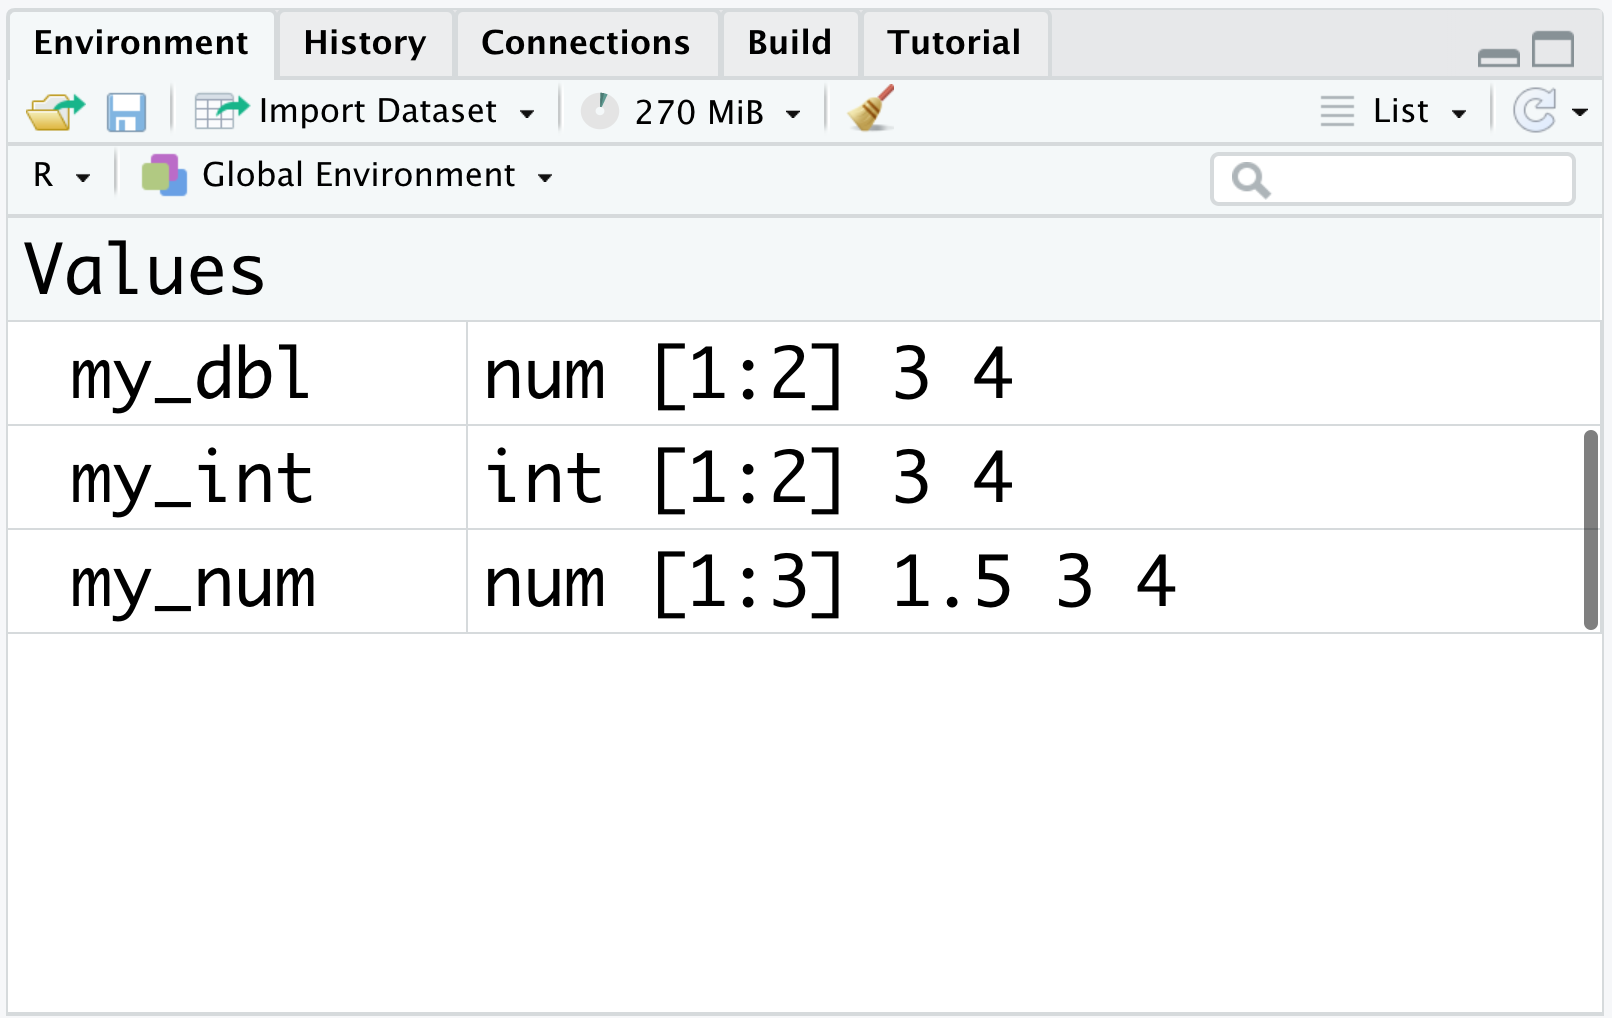
\includegraphics[width=0.7\linewidth]{pics/2en3} 

}

\caption{Different storage types}\label{fig:en13}
\end{figure}

From the picture above, you can see that the values of \texttt{my\_int} are still 3 and 4, which are the same as those of \texttt{my\_dbl}. The difference between these two vectors is that \texttt{my\_int} is an integer vector since its internal storage type is integer, and such a storage type offers great \emph{memory savings} compared to doubles.

Notice that a numeric vector's internal storage type is consistent. Say if you assign multiple numeric values to an object, even when you assign an ``L'' to most values, as long as the object obtains at least one decimal value, the vector will be stored in R as double. This rule also implies that any numeric vector containing at least one decimal value cannot be transformed to an integer vector.

\begin{Shaded}
\begin{Highlighting}[]
\NormalTok{my\_num2 }\OtherTok{\textless{}{-}} \FunctionTok{c}\NormalTok{(}\FloatTok{1.5}\NormalTok{, 3L, 4L)}
\FunctionTok{typeof}\NormalTok{(my\_num2) }
\CommentTok{\#\textgreater{} [1] "double"}
\FunctionTok{class}\NormalTok{(my\_num2)}
\CommentTok{\#\textgreater{} [1] "numeric"}
\end{Highlighting}
\end{Shaded}

Moreover, as you can see by running the code below, whenever you put an ``L'' after an decimal value, you will get the warning and the storage type will remain \texttt{double}.

\begin{Shaded}
\begin{Highlighting}[]
\NormalTok{my\_num3 }\OtherTok{\textless{}{-}} \FunctionTok{c}\NormalTok{(}\FloatTok{1.5}\NormalTok{L, 3L, 4L)}
\FunctionTok{typeof}\NormalTok{(my\_num3)}
\CommentTok{\#\textgreater{} [1] "double"}
\FunctionTok{class}\NormalTok{(my\_num3)}
\CommentTok{\#\textgreater{} [1] "numeric"}
\end{Highlighting}
\end{Shaded}

In conclusion, all the numeric vectors will be stored as \texttt{double} by default. If all values in a numeric vector are integers, you can convert this numeric vector into an integer vector, and the storage type of this vector will be \texttt{integer}, which can save memories compared to doubles. That being said, don't get confused: both double and integer vectors belong to numeric vectors.

\begin{infobox}{caution}
Despite the differences between integers and doubles, you can usually ignore their differences unless you are working on a very big data set. R will automatically convert objects between integers and doubles when necessary.

\end{infobox}

\hypertarget{printing}{%
\subsection{Printing}\label{printing}}

Now, you have learned numeric vectors along with their possible storage types. In this part, let's discuss how you can customize the output digit of a number via printing. Let's start with \texttt{pi}, which is a mathematical constant you may be familiar with. \texttt{pi} is also an internal numeric vector available for use in R, meaning that it will appear in the environment panel without requiring you to assign it to a name.

\begin{Shaded}
\begin{Highlighting}[]
\NormalTok{pi}
\CommentTok{\#\textgreater{} [1] 3.141593}
\end{Highlighting}
\end{Shaded}

As you can see from the output, R prints out 7 \textbf{significant digits} by default, though in fact we need infinitely many digits to faithfully represent \texttt{pi}. To print out an object with a customized significant digit number, you can use the \texttt{print()} function that contains useful argument called \texttt{digits}, which controls the number of significant digits to be printed. Let's see the following examples.

You can try the following examples.

\begin{Shaded}
\begin{Highlighting}[]
\FunctionTok{print}\NormalTok{(pi, }\AttributeTok{digits =} \DecValTok{20}\NormalTok{)          }\CommentTok{\#print pi for 20 significant digits}
\CommentTok{\#\textgreater{} [1] 3.141592653589793116}
\FunctionTok{print}\NormalTok{(pi, }\AttributeTok{digits =} \DecValTok{4}\NormalTok{)           }\CommentTok{\#print pi for 4 significant digits}
\CommentTok{\#\textgreater{} [1] 3.142}
\end{Highlighting}
\end{Shaded}

\begin{infobox}{caution}

Note that the \texttt{round()} function also has an argument \texttt{digits}, which has a \textbf{different} meaning, representing the number of digits after the decimal point.

\begin{Shaded}
\begin{Highlighting}[]
\FunctionTok{print}\NormalTok{(pi, }\AttributeTok{digits =} \DecValTok{4}\NormalTok{)           }\CommentTok{\#print pi for 4 significant digits}
\CommentTok{\#\textgreater{} [1] 3.142}
\FunctionTok{round}\NormalTok{(pi, }\AttributeTok{digits =} \DecValTok{4}\NormalTok{)           }\CommentTok{\#round pi to 4 decimal places}
\CommentTok{\#\textgreater{} [1] 3.1416}
\end{Highlighting}
\end{Shaded}

\end{infobox}

You may be wondering whether happens if \texttt{digits} is larger than the number of the actual significant digits of a number. Let's try the following example.

\begin{Shaded}
\begin{Highlighting}[]
\FunctionTok{print}\NormalTok{(}\FloatTok{1.2}\NormalTok{, }\AttributeTok{digits =} \DecValTok{5}\NormalTok{)}
\CommentTok{\#\textgreater{} [1] 1.2}
\end{Highlighting}
\end{Shaded}

Clearly, the \texttt{print()} function will print out at most the significant digits of the number.

When you print a vector with more than one element, the same number of decimal places is printed for all elements. In this case, the \texttt{digits} parameter represents the \textbf{minimum} number of significant digits, and that at least one element will be encoded with that minimum number.

\begin{Shaded}
\begin{Highlighting}[]
\FunctionTok{print}\NormalTok{(}\FunctionTok{c}\NormalTok{(pi, }\FunctionTok{exp}\NormalTok{(}\DecValTok{1}\NormalTok{), }\FunctionTok{log}\NormalTok{(}\DecValTok{2}\NormalTok{)), }\AttributeTok{digits =} \DecValTok{4}\NormalTok{)}
\CommentTok{\#\textgreater{} [1] 3.1416 2.7183 0.6931}
\FunctionTok{print}\NormalTok{(}\FunctionTok{c}\NormalTok{(pi, }\FunctionTok{exp}\NormalTok{(}\DecValTok{1}\NormalTok{), }\FunctionTok{log}\NormalTok{(}\DecValTok{2}\NormalTok{), }\FunctionTok{exp}\NormalTok{(}\SpecialCharTok{{-}}\DecValTok{5}\NormalTok{)), }\AttributeTok{digits =} \DecValTok{4}\NormalTok{)}
\CommentTok{\#\textgreater{} [1] 3.141593 2.718282 0.693147 0.006738}
\FunctionTok{print}\NormalTok{(}\FunctionTok{c}\NormalTok{(}\DecValTok{20000}\NormalTok{, }\FloatTok{1.2}\NormalTok{, }\FloatTok{2.34}\NormalTok{), }\AttributeTok{digits =} \DecValTok{3}\NormalTok{)}
\CommentTok{\#\textgreater{} [1] 20000.00     1.20     2.34}
\end{Highlighting}
\end{Shaded}

As you can imagine, the \texttt{print()} function will be very useful in creating tables that look more streamlined.

\hypertarget{exercises-3}{%
\subsection{Exercises}\label{exercises-3}}

Write the R code to complete the following tasks.

\begin{enumerate}
\def\labelenumi{\arabic{enumi}.}
\item
  Create a numeric vector named \texttt{vec\_1} with values \((2, 4, 6, 8)\), get its length, find out its class, and get its storage type.
\item
  For the numeric vector \texttt{vec\_2\ \textless{}-\ c(1,\ 3,\ 7,\ 10)}, get the value of the 3rd element, multiple the 3rd element by 5, and verify the change.
\item
  Create a vector \texttt{vec\_3} where each element is twice the corresponding element in \texttt{vec\_1} minus half the corresponding element in \texttt{vec\_2}.
\item
  Create an integer vector \texttt{int\_1} that contains integers \((2, 4, 6, 8)\). Check its class and storage type.
\item
  Print out the vector \((e, e^2, e^3)\) with 5 significant digits.
\end{enumerate}

\hypertarget{intro-char-vector}{%
\section{Introduction to Character Vectors}\label{intro-char-vector}}

After familiarizing yourself with the numeric vectors in Section \ref{intro-num-vector}, we will introduce another member of the atomic vector family: character vectors.

\hypertarget{create-character-vector}{%
\subsection{Creation, class and storage type}\label{create-character-vector}}

A \textbf{character vector} is another type of atomic vector (where all elements are of the same type). In a character vector, the value of each element is of character type, which means each element is a string. A string is a sequence of characters (including letters, numbers, or symbols) surrounded by the double quotes ("") or single quotes (''). For consistency, we will stick with double quotes in this book.

The first example: if the word book is surrounded by a pair of double quotes, then it is a string, and \texttt{"book"} is a character vector with length 1. The value of \texttt{"book"} is the string itself. Notice that here \texttt{"book"} is a vector \textbf{without} a name since we have not assigned its value to a name, which will be introduced shortly. You can then verify the number of strings in this vector by using \texttt{length()} and verify the vector type by using \texttt{class()}.

\begin{Shaded}
\begin{Highlighting}[]
\StringTok{"book"} 
\CommentTok{\#\textgreater{} [1] "book"}
\FunctionTok{length}\NormalTok{(}\StringTok{"book"}\NormalTok{)}
\CommentTok{\#\textgreater{} [1] 1}
\FunctionTok{class}\NormalTok{(}\StringTok{"book"}\NormalTok{)}
\CommentTok{\#\textgreater{} [1] "character"}
\end{Highlighting}
\end{Shaded}

Now the \texttt{class()} function will return \texttt{character}, which shows that \texttt{"book"} is a character vector.

After assigning the value to the name r02pro, you have created a new character vector \texttt{r02pro} with ``book'' as the value.

\begin{Shaded}
\begin{Highlighting}[]
\NormalTok{r02pro }\OtherTok{\textless{}{-}} \StringTok{"book"} 
\NormalTok{r02pro}
\CommentTok{\#\textgreater{} [1] "book"}
\FunctionTok{class}\NormalTok{(r02pro)}
\CommentTok{\#\textgreater{} [1] "character"}
\end{Highlighting}
\end{Shaded}

\begin{infobox}{caution}

Double quotes need to be paired in strings. If you miss the right double quote, R will show a plus on the next line, waiting for you to finish the command. If this happens, you can either enter the matching double quote, or press ESC to escape this command.

\begin{figure}

{\centering 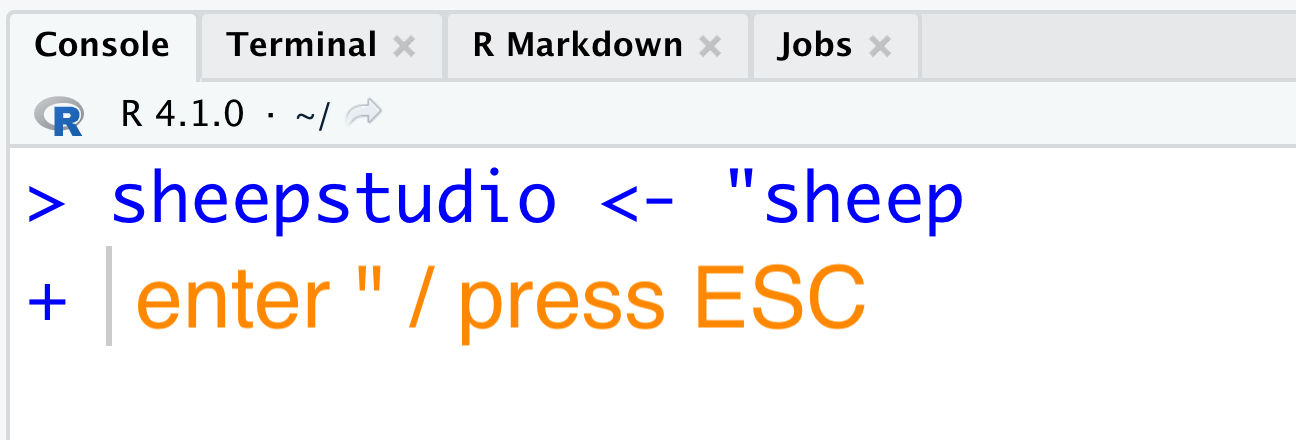
\includegraphics[width=0.7\linewidth]{pics/2quo} 

}

\caption{Miss the right quotation mark}\label{fig:quo}
\end{figure}

\end{infobox}

Next, let's create a numeric vector \texttt{num\_vec} with number 708. After adding a pair of double quotes around the number 708, ``708'' has converted to a string now. You can assign the value ``708'' to a name (say char\_vec), which will create a new character vector named \texttt{char\_vec}. Don't forget to check the vector type by using \texttt{class()} if you are not sure.

\begin{Shaded}
\begin{Highlighting}[]
\NormalTok{num\_vec }\OtherTok{\textless{}{-}} \DecValTok{708}
\NormalTok{char\_vec }\OtherTok{\textless{}{-}} \StringTok{"708"} 
\FunctionTok{class}\NormalTok{(num\_vec)}
\CommentTok{\#\textgreater{} [1] "numeric"}
\FunctionTok{class}\NormalTok{(char\_vec)}
\CommentTok{\#\textgreater{} [1] "character"}
\end{Highlighting}
\end{Shaded}

Also, strings can contain symbols. For example, you can create a character vector with ``gph\&708''.

\begin{Shaded}
\begin{Highlighting}[]
\NormalTok{char\_vec2 }\OtherTok{\textless{}{-}} \StringTok{"gph\&708"}
\FunctionTok{class}\NormalTok{(char\_vec2)}
\CommentTok{\#\textgreater{} [1] "character"}
\end{Highlighting}
\end{Shaded}

In conclusion, if characters (including letters, numbers, and symbols) are surrounded by double quotes, it will be interpreted as a string by the R language.

Similar to a numeric vector, you can have multiple elements in a character vector, using the \texttt{c()} function to combine several strings into a single vector. You can verify the number of elements in a vector by using the \texttt{length()} function.

Now we know how to obtain the length of a vector, but what about the length of a single element within a given vector? Function \texttt{nchar()} can help us with that, as you will get the number of \textbf{characters} in a string.

\begin{Shaded}
\begin{Highlighting}[]
\NormalTok{animals }\OtherTok{\textless{}{-}} \FunctionTok{c}\NormalTok{(}\StringTok{"sheep\%29"}\NormalTok{, }\StringTok{"bear$11"}\NormalTok{, }\StringTok{"monkey@66"}\NormalTok{)}
\NormalTok{animals}
\CommentTok{\#\textgreater{} [1] "sheep\%29"  "bear$11"   "monkey@66"}
\FunctionTok{length}\NormalTok{(animals)}
\CommentTok{\#\textgreater{} [1] 3}
\FunctionTok{nchar}\NormalTok{(animals)}
\CommentTok{\#\textgreater{} [1] 8 7 9}
\end{Highlighting}
\end{Shaded}

As shown in the example, we can see that there are three elements in the \texttt{animals} vector, and string ``sheep\%29'' has a length of 8 (including 5 characters, 1 symbol, and 2 numbers). Similarly, ``bear\$11'' and ``\href{mailto:monkey@66}{\nolinkurl{monkey@66}}'' have a length of 7 and 9, and you can check it by yourself with the \texttt{nchar()} function.

Same as the numeric vector, you can use the \texttt{typeof()} function to find the internal storage type of a character vector. All the character vectors will be stored as the \textbf{character} in R. You can check the storage type of some character vectors we created before.

\begin{Shaded}
\begin{Highlighting}[]
\FunctionTok{typeof}\NormalTok{(char\_vec)}
\CommentTok{\#\textgreater{} [1] "character"}
\FunctionTok{typeof}\NormalTok{(animals)}
\CommentTok{\#\textgreater{} [1] "character"}
\end{Highlighting}
\end{Shaded}

Finally, you can use the \texttt{vector(mode,\ length)} function to create a character vector of certain length.

\begin{Shaded}
\begin{Highlighting}[]
\FunctionTok{vector}\NormalTok{(}\StringTok{"character"}\NormalTok{, }\DecValTok{6}\NormalTok{)}
\CommentTok{\#\textgreater{} [1] "" "" "" "" "" ""}
\end{Highlighting}
\end{Shaded}

Note that the default value is an empty string for all elements.

\hypertarget{case}{%
\subsection{Change case}\label{case}}

In character vectors, each string can contain both uppercase and lowercase letters. You can unify the cases of all letters inside a vector. Let's review the character vector \texttt{four\_strings} first,

\begin{Shaded}
\begin{Highlighting}[]
\NormalTok{four\_strings }\OtherTok{\textless{}{-}} \FunctionTok{c}\NormalTok{(}\StringTok{"This"}\NormalTok{, }\StringTok{"is"}\NormalTok{, }\StringTok{"R02\#"}\NormalTok{, }\StringTok{"$Pro"}\NormalTok{)}
\NormalTok{four\_strings}
\CommentTok{\#\textgreater{} [1] "This" "is"   "R02\#" "$Pro"}
\end{Highlighting}
\end{Shaded}

As one could observe, the vector \texttt{four\_strings} contains a mix of uppercase, lowercase, numbers, and symbols. In order to convert all convertible characters in each string to lowercase, you can use the \texttt{tolower()} function.

The converted result can be shown directly, or saved as a new vector with your name of preference. For example, after \texttt{four\_strings} is passed to \texttt{tolower()}, the returned result was saved to \texttt{lower\_strings}.

\begin{Shaded}
\begin{Highlighting}[]
\NormalTok{lower\_strings }\OtherTok{\textless{}{-}} \FunctionTok{tolower}\NormalTok{(four\_strings)}
\NormalTok{lower\_strings}
\CommentTok{\#\textgreater{} [1] "this" "is"   "r02\#" "$pro"}
\end{Highlighting}
\end{Shaded}

One should also notice that, numbers and symbols within a string will not be changed, as they are non-alphabetic characters.
The opposite operation of \texttt{tolower()} is \texttt{toupper()}, which converts all characters in the vector to uppercase.

\begin{Shaded}
\begin{Highlighting}[]
\NormalTok{upper\_strings }\OtherTok{\textless{}{-}} \FunctionTok{toupper}\NormalTok{(four\_strings)}
\NormalTok{upper\_strings}
\CommentTok{\#\textgreater{} [1] "THIS" "IS"   "R02\#" "$PRO"}
\end{Highlighting}
\end{Shaded}

\hypertarget{review-of-getting-help-in-r}{%
\subsection{Review of getting help in R}\label{review-of-getting-help-in-r}}

In Section \ref{get-help}, we introduced three common ways to get help in R, which can help you know more about a particular function. In this section, we will review these methods by taking \texttt{toupper} and \texttt{tolower} as examples.

\begin{itemize}
\tightlist
\item
  Use a question mark followed by the function name \texttt{?tolower}
\item
  Use help function \texttt{help(tolower)}
\item
  Use the help window in RStudio
\end{itemize}

Use any of the methods listed above to get the documentation for the function \texttt{tolower()}, and let's take a detailed look at it.

Different from the documentation of the \texttt{sign()} function, you will the title is named ``Character Translation and Casefolding'' (Figure \ref{fig:help1}).

\begin{figure}

{\centering 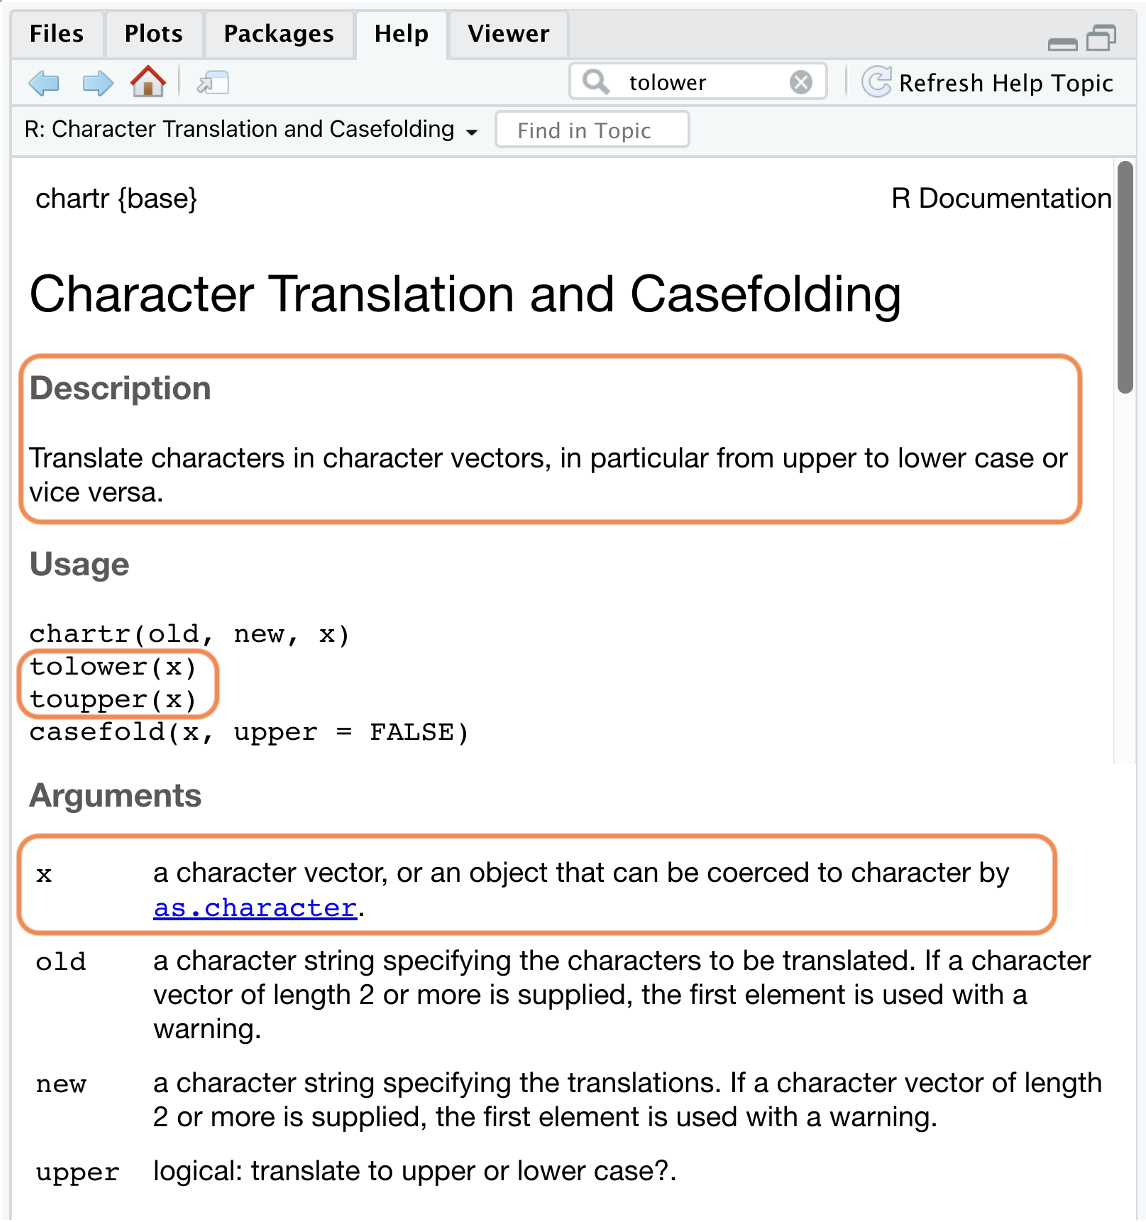
\includegraphics[width=0.7\linewidth]{pics/2help1} 

}

\caption{Help (I)}\label{fig:help1}
\end{figure}

\begin{itemize}
\tightlist
\item
  The \emph{Description} part describes the general purpose of this function. In this example, all functions introduced in this documentation translate characters in a character vector (from upper to lower case or vice versa).
\item
  The \emph{Usage} part shows the expected syntax. This section may contain multiple functions that share similar usage, but with different number and format of input. For example, \texttt{chartr} is expecting three arguments, which is \texttt{old},\texttt{new} and \texttt{x}, respectively, but \texttt{tolower} and \texttt{toupper} functions is only taking one argument \texttt{x}.
\item
  The \emph{Arguments} part provides detailed explanation for argument. Depending on the function, argument could be different from data type to input length, and it is best to read them individually. For our example, you can focus on the explanation of \texttt{x} for \texttt{tolower} and \texttt{toupper} functions for now, as this is the only required input for both of them.
\end{itemize}

Next, let's move to the \emph{Details} part,

\begin{figure}

{\centering 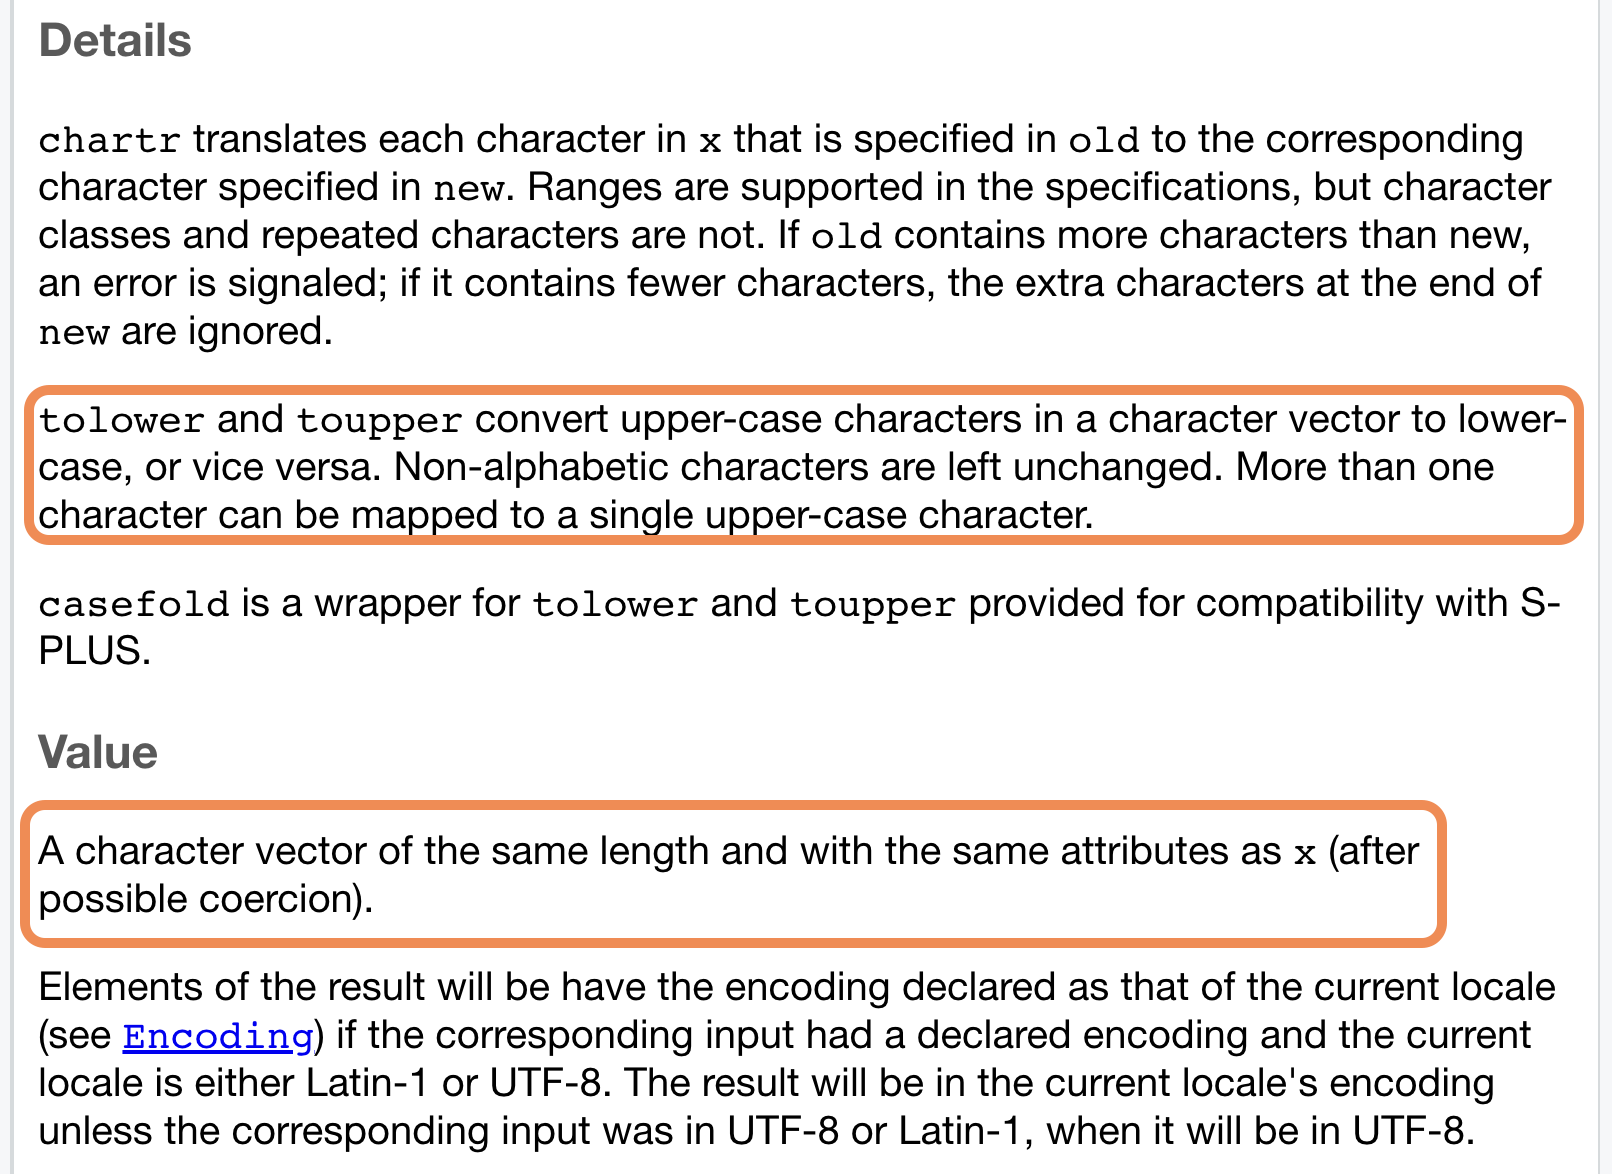
\includegraphics[width=0.7\linewidth]{pics/2help2} 

}

\caption{Help (II)}\label{fig:help2}
\end{figure}

\begin{itemize}
\tightlist
\item
  The \emph{Details} part explains the mechanism of the functions, as well as what each of them could achieve.
\item
  The \emph{Value} part shows the result that the function would return, with specified data attributes and types. For \texttt{tolower} and \texttt{toupper}, since we only covert the cases of characters, the returned character vector will share the same \texttt{length()} as the input vector.
\end{itemize}

\begin{figure}

{\centering 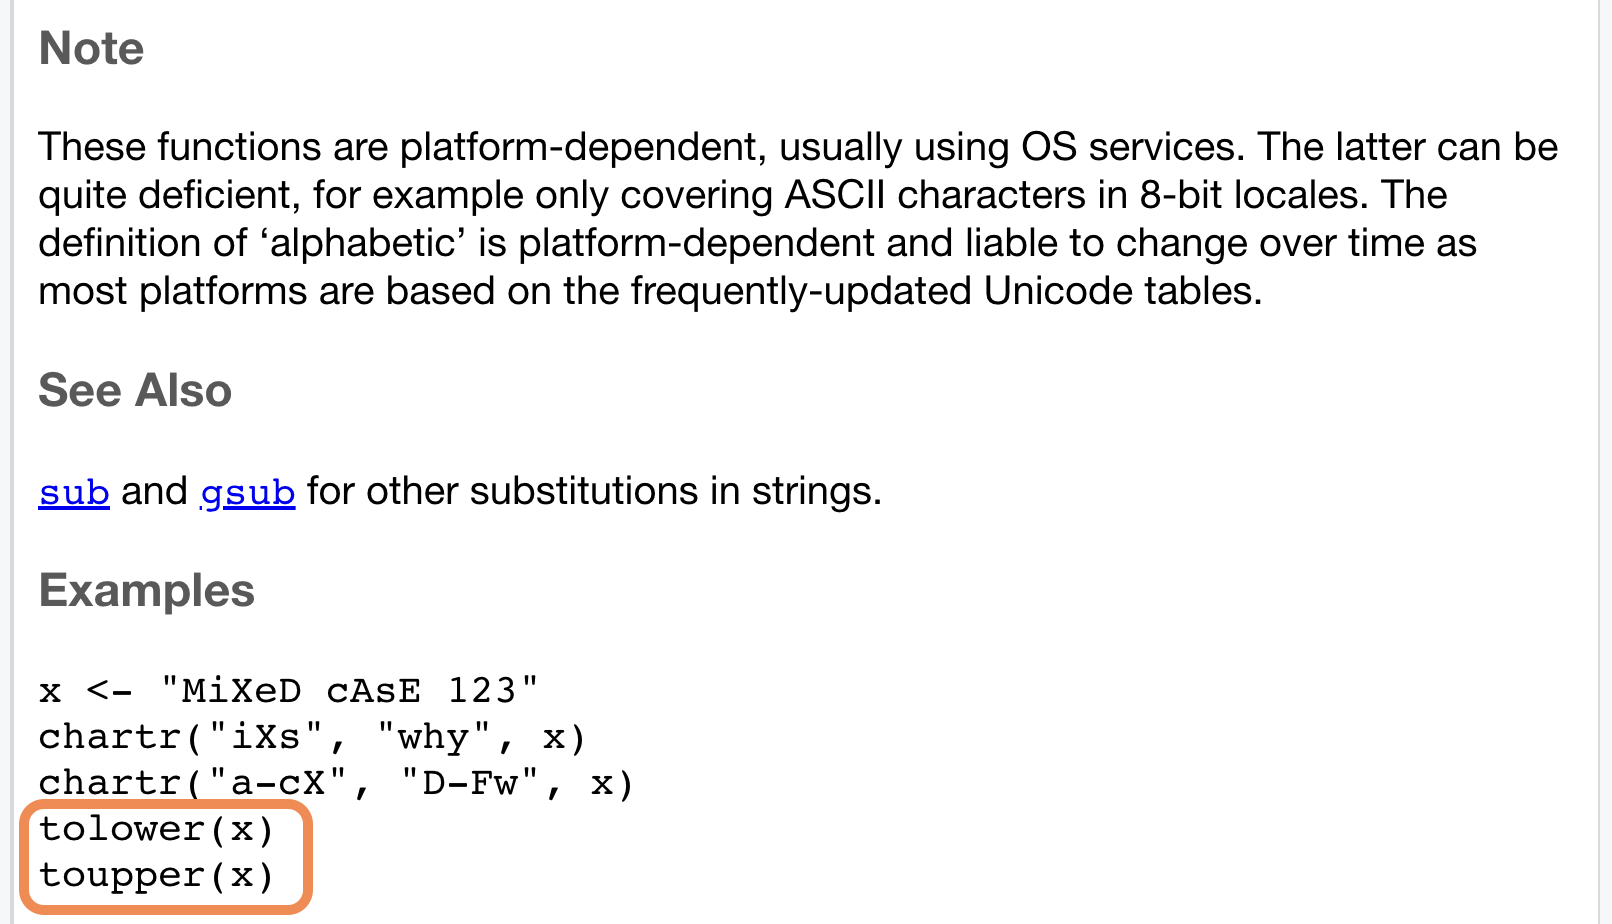
\includegraphics[width=0.7\linewidth]{pics/2help3} 

}

\caption{Help (III)}\label{fig:help3}
\end{figure}

In the last part of the documentation, you can see the notes in the \emph{Note} part and some functions related to functions introduced in the \emph{See Also} part. Remember to try some sample codes in the \emph{Examples} part, and implement your own codes with the help of the examples.

At the end of this section, let us review the environment panel. You can see all the character vectors \textbf{with names} in this section. Notice that now the vector type has been changed to \emph{chr} (here \emph{chr} is short for character).

\begin{figure}

{\centering 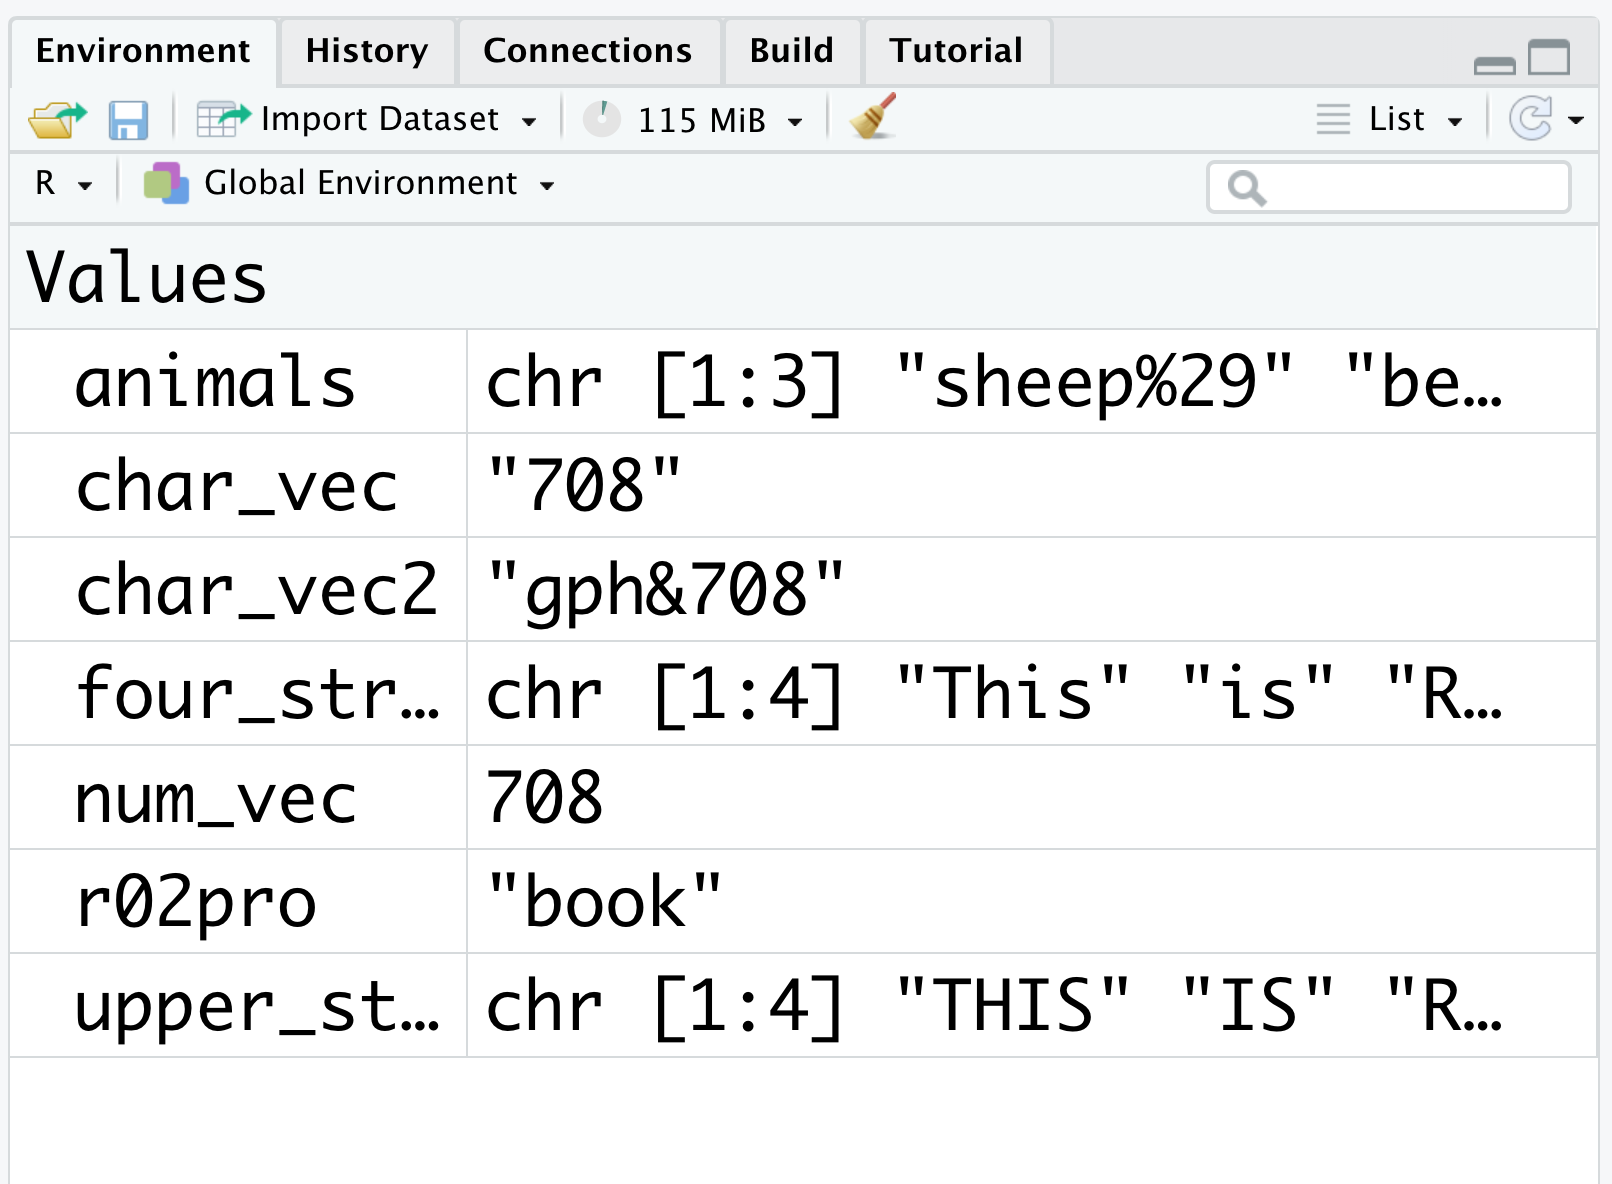
\includegraphics[width=0.7\linewidth]{pics/2char} 

}

\caption{Character vectors}\label{fig:char}
\end{figure}

You can also see the list of all the named objects by using \texttt{ls()} function.

\begin{Shaded}
\begin{Highlighting}[]
\FunctionTok{ls}\NormalTok{()}
\CommentTok{\#\textgreater{} [1] "animals"       "char\_vec"      "char\_vec2"     "four\_strings" }
\CommentTok{\#\textgreater{} [5] "lower\_strings" "num\_vec"       "r02pro"        "upper\_strings"}
\end{Highlighting}
\end{Shaded}

\hypertarget{exercises-4}{%
\subsection{Exercises}\label{exercises-4}}

\begin{enumerate}
\def\labelenumi{\arabic{enumi}.}
\item
  Write R code to create a numeric vector named \texttt{vec\_1} with values \texttt{7\ 24\ 8\ 26}, get its length, and find out its type.
\item
  Write R code to create a character vector named \texttt{char\_1} with values \texttt{"I"}, \texttt{"am"}, \texttt{"learning"}, \texttt{"R!"}, get its length, find out its type, and concatenate the vector into a single string with space as the separator.
\item
  For the \texttt{char\_1} defined in Q2, find the number of characters in each string, and convert each string to upper case.
\item
  Create a length-2 logical vector representing whether \texttt{vec\_1} and \texttt{char\_1} are of character type.
\end{enumerate}

\hypertarget{intro-logi-vector}{%
\section{Introduction to Logical Vectors}\label{intro-logi-vector}}

Having learning numeric vectors (Section \ref{intro-num-vector}) and character vectors (Section \ref{intro-char-vector}), it is time to master \textbf{logical vectors}, which is another important type of atomic vectors, containing only logical values.

\hypertarget{create-logical-vector}{%
\subsection{Logical vectors: creation by comparisons, class, and storage type}\label{create-logical-vector}}

A \textbf{logical vector} is an atomic vector containing only \textbf{logical values}, namely \texttt{TRUE} and \texttt{FALSE}. Logical vectors are most omnipresent when we check whether a comparison statement is true or false. Generally, comparisons are more common between numeric vectors, since it is easy to compare numbers, so we will take the comparisons between numeric vectors as examples in this section.

For two length-1 vector, the comparison is simply done between the only element of each vector. Let's create a numeric vector \texttt{x} with value \texttt{3}, and then compare it with \texttt{2} and \texttt{1}. (Here \texttt{2} and \texttt{1} are both length-1 numeric vectors)

\begin{Shaded}
\begin{Highlighting}[]
\NormalTok{x }\OtherTok{\textless{}{-}} \DecValTok{3}
\NormalTok{x }\SpecialCharTok{\textless{}} \DecValTok{2}
\CommentTok{\#\textgreater{} [1] FALSE}
\NormalTok{x }\SpecialCharTok{\textgreater{}} \DecValTok{1}
\CommentTok{\#\textgreater{} [1] TRUE}
\end{Highlighting}
\end{Shaded}

The value of \texttt{x\ \textless{}\ 2} is \texttt{FALSE} since 3 is not smaller than 2, and the value of \texttt{x\ \textgreater{}\ 1} is \texttt{TRUE} since 3 is larger than 1. So \texttt{x\ \textless{}\ 2} and \texttt{x\ \textgreater{}\ 1} are both vectors of length 1. Just like numeric and character vectors, you can check the class, length, and storage type of the result of this comparison. Let's take \texttt{x\ \textgreater{}\ 1} for example.

\begin{Shaded}
\begin{Highlighting}[]
\FunctionTok{class}\NormalTok{(x }\SpecialCharTok{\textgreater{}} \DecValTok{1}\NormalTok{)}
\CommentTok{\#\textgreater{} [1] "logical"}
\FunctionTok{length}\NormalTok{(x }\SpecialCharTok{\textgreater{}} \DecValTok{1}\NormalTok{)}
\CommentTok{\#\textgreater{} [1] 1}
\FunctionTok{typeof}\NormalTok{(x }\SpecialCharTok{\textgreater{}} \DecValTok{1}\NormalTok{)}
\CommentTok{\#\textgreater{} [1] "logical"}
\end{Highlighting}
\end{Shaded}

In addition, you can assign values of logical vectors to names for future use.

\begin{Shaded}
\begin{Highlighting}[]
\NormalTok{big\_1 }\OtherTok{\textless{}{-}}\NormalTok{ x }\SpecialCharTok{\textgreater{}} \DecValTok{1}
\NormalTok{big\_1}
\FunctionTok{class}\NormalTok{(big\_1)}
\FunctionTok{typeof}\NormalTok{(big\_1)}
\end{Highlighting}
\end{Shaded}

Now, it is clear that \texttt{x\ \textgreater{}\ 1} and \texttt{big\_1} are both logical vectors with length of 1.

There are a few other commonly used operators for doing comparisons, which all result in \texttt{TRUE} when the statement is correct, and \texttt{FALSE} otherwise.

\begin{Shaded}
\begin{Highlighting}[]
\NormalTok{x }\SpecialCharTok{\textless{}} \DecValTok{2}      \CommentTok{\#less than}
\CommentTok{\#\textgreater{} [1] FALSE}
\NormalTok{x }\SpecialCharTok{\textless{}=} \DecValTok{2}     \CommentTok{\#less than or equal to}
\CommentTok{\#\textgreater{} [1] FALSE}
\NormalTok{x }\SpecialCharTok{\textgreater{}} \DecValTok{1}      \CommentTok{\#bigger than}
\CommentTok{\#\textgreater{} [1] TRUE}
\NormalTok{x }\SpecialCharTok{\textgreater{}=} \DecValTok{1}     \CommentTok{\#bigger than or equal to}
\CommentTok{\#\textgreater{} [1] TRUE}
\NormalTok{x }\SpecialCharTok{==} \DecValTok{3}     \CommentTok{\#equal to}
\CommentTok{\#\textgreater{} [1] TRUE}
\CommentTok{\#x = 3     \#another assignment operator in addition to \textasciigrave{}\textless{}{-}\textasciigrave{}, NOT comparison}
\NormalTok{x }\SpecialCharTok{!=} \DecValTok{3}     \CommentTok{\#not equal to}
\CommentTok{\#\textgreater{} [1] FALSE}
\end{Highlighting}
\end{Shaded}

Note that if you want to check whether two vectors are equal, you have to use \textbf{two equal signs} (with no space in-between) as a single operator, which is \texttt{==}, to do comparisons. If only one equal sign is used, it would work as an assignment operator. In addition, you can use an exclamation mark together with one equal sign, which is \texttt{!=}, to find out whether two vectors are not equal.

In addition to making comparisons involving vectors of length 1, you can also do it with vectors containing more than 1 elements. When we make comparisons between two vectors that contain more than 1 elements, R will make an \textbf{element-wise} comparison just like the arithmetic operations between two numeric vectors in Section \ref{operation-recycling}.

\begin{Shaded}
\begin{Highlighting}[]
\NormalTok{x2 }\OtherTok{\textless{}{-}} \FunctionTok{c}\NormalTok{(}\DecValTok{1}\NormalTok{, }\DecValTok{2}\NormalTok{, }\DecValTok{6}\NormalTok{)}
\NormalTok{x3 }\OtherTok{\textless{}{-}} \FunctionTok{c}\NormalTok{(}\DecValTok{2}\NormalTok{, }\DecValTok{2}\NormalTok{, }\DecValTok{4}\NormalTok{)}
\NormalTok{logi\_1 }\OtherTok{\textless{}{-}}\NormalTok{ x2 }\SpecialCharTok{\textless{}=}\NormalTok{ x3}
\NormalTok{logi\_1 }
\CommentTok{\#\textgreater{} [1]  TRUE  TRUE FALSE}
\end{Highlighting}
\end{Shaded}

As \texttt{x2} and \texttt{x3} are of the same length, \textbf{element-wise} comparison will be applied. The result of this comparison \texttt{logi\_1} will be a logical vector of same length, and only contain \texttt{TRUE} and \texttt{FALSE.} You can also manually check that the values of \texttt{logi\_1} agree with the comparisons \texttt{1\ \textless{}=\ 2}, \texttt{2\ \textless{}=\ 2}, and \texttt{6\ \textless{}=\ 4}.

Similar to the arithmetic operations on numeric vectors, the \textbf{recycling rule} (introduced in Section \ref{operation-recycling}) also applies to the comparison when the two vectors do not have the same length. This recycling is most often used for a comparison between a vector \textbf{with length greater than 1} and a vector \textbf{with length of 1}. Let's see an example.

\begin{Shaded}
\begin{Highlighting}[]
\NormalTok{x3 }\OtherTok{\textless{}{-}} \FunctionTok{c}\NormalTok{(}\DecValTok{2}\NormalTok{, }\DecValTok{2}\NormalTok{, }\DecValTok{4}\NormalTok{)}
\NormalTok{x3 }\SpecialCharTok{!=} \DecValTok{2} 
\CommentTok{\#\textgreater{} [1] FALSE FALSE  TRUE}
\end{Highlighting}
\end{Shaded}

Here, \texttt{x3} is a numeric vector with length of 3, and \texttt{2} is a numeric vector of length 1. From the result, you can see that \texttt{2} is compared with each element in \texttt{x3}, producing a length-3 logical vector. You can simply check the values by doing the following comparisons: \texttt{2\ !=\ 2}, \texttt{2\ !=\ 2} and \texttt{4\ !=\ 2}.

Now you must be familiar with logical vectors. Similar to numeric vectors and character vector, you can also use the \texttt{c()} function along with the logical values \texttt{TRUE} (or \texttt{T} for short) and \texttt{FALSE} (or \texttt{F} for short) as elements.

\begin{Shaded}
\begin{Highlighting}[]
\NormalTok{logi\_2 }\OtherTok{\textless{}{-}} \FunctionTok{c}\NormalTok{(}\ConstantTok{TRUE}\NormalTok{, }\ConstantTok{FALSE}\NormalTok{, }\ConstantTok{TRUE}\NormalTok{)}
\NormalTok{logi\_2}
\CommentTok{\#\textgreater{} [1]  TRUE FALSE  TRUE}
\FunctionTok{class}\NormalTok{(logi\_2)}
\CommentTok{\#\textgreater{} [1] "logical"}
\end{Highlighting}
\end{Shaded}

The values of logical vectors can also be \texttt{T} or \texttt{F}. You can check the class of \texttt{logi\_3} by using \texttt{class()}.

\begin{Shaded}
\begin{Highlighting}[]
\NormalTok{logi\_3 }\OtherTok{\textless{}{-}} \FunctionTok{c}\NormalTok{(F, T, F, T)}
\NormalTok{logi\_3}
\FunctionTok{class}\NormalTok{(logi\_3)}
\FunctionTok{typeof}\NormalTok{(logi\_3)}
\end{Highlighting}
\end{Shaded}

\begin{infobox}{caution}

It is worth emphasizing that, in creating numeric vectors and logical vectors, quotation marks aren't necessary like they are in creating character vectors. If you put quotation marks around \texttt{TRUE} or \texttt{FALSE}, you will create a character vector instead.

\begin{Shaded}
\begin{Highlighting}[]
\NormalTok{char\_1 }\OtherTok{\textless{}{-}} \FunctionTok{c}\NormalTok{(}\StringTok{"TRUE"}\NormalTok{, }\StringTok{"FALSE"}\NormalTok{, }\StringTok{"TRUE"}\NormalTok{)}
\NormalTok{char\_1}
\CommentTok{\#\textgreater{} [1] "TRUE"  "FALSE" "TRUE"}
\FunctionTok{class}\NormalTok{(char\_1)}
\CommentTok{\#\textgreater{} [1] "character"}
\end{Highlighting}
\end{Shaded}

\end{infobox}

It is worth mentioning that, R is case-sensitive in terms of the expression of \texttt{TRUE} and \texttt{FALSE}. Any expression other than \texttt{TRUE}, \texttt{FALSE}, \texttt{T}, or \texttt{F} will be recognized as character values or name of an object in R, not logical values. Please see the example below.

\begin{Shaded}
\begin{Highlighting}[]
\CommentTok{\# Valid Expression }
\FunctionTok{class}\NormalTok{(}\FunctionTok{c}\NormalTok{(}\ConstantTok{TRUE}\NormalTok{, T))}
\CommentTok{\#\textgreater{} [1] "logical"}

\CommentTok{\# Invalid Expression}
\FunctionTok{class}\NormalTok{(true)}
\CommentTok{\#\textgreater{} Error in eval(expr, envir, enclos): object \textquotesingle{}true\textquotesingle{} not found}
\FunctionTok{class}\NormalTok{(True)}
\CommentTok{\#\textgreater{} Error in eval(expr, envir, enclos): object \textquotesingle{}True\textquotesingle{} not found}
\FunctionTok{class}\NormalTok{(}\StringTok{"true"}\NormalTok{)}
\CommentTok{\#\textgreater{} [1] "character"}
\end{Highlighting}
\end{Shaded}

Finally, you can use the \texttt{vector(mode,\ length)} function to create a logical vector of certain length.

\begin{Shaded}
\begin{Highlighting}[]
\FunctionTok{vector}\NormalTok{(}\StringTok{"logical"}\NormalTok{, }\DecValTok{2}\NormalTok{)}
\end{Highlighting}
\end{Shaded}

Note that the default value is \texttt{FALSE}.

\hypertarget{logical-vectors-creation-when-testing-for-types}{%
\subsection{Logical vectors: creation when testing for types}\label{logical-vectors-creation-when-testing-for-types}}

In addition to comparison operations, another situation that you will encounter logical vectors is when we test whether an object belongs to certain type.

First of all, you can use \texttt{is.numeric()} to check whether an object is numeric, i.e.~can be interpreted as numbers. It will return \texttt{TRUE} if the object is numeric, and will otherwise return \texttt{FALSE}. Note that both double vectors and integer vectors (Section \ref{storage-type}) are numeric since they can both be interpreted as numbers. To further differentiate between double vectors and integer vectors, you can use \texttt{is.double()} and \texttt{is.integer()}.

\begin{Shaded}
\begin{Highlighting}[]
\NormalTok{x1 }\OtherTok{\textless{}{-}} \FunctionTok{c}\NormalTok{(}\DecValTok{1}\NormalTok{, }\DecValTok{2}\NormalTok{)}
\NormalTok{x2 }\OtherTok{\textless{}{-}} \FunctionTok{c}\NormalTok{(1L, 2L)}
\FunctionTok{c}\NormalTok{(}\FunctionTok{is.numeric}\NormalTok{(x1), }\FunctionTok{is.double}\NormalTok{(x1), }\FunctionTok{is.integer}\NormalTok{(x1))}
\CommentTok{\#\textgreater{} [1]  TRUE  TRUE FALSE}
\FunctionTok{c}\NormalTok{(}\FunctionTok{is.numeric}\NormalTok{(x2), }\FunctionTok{is.double}\NormalTok{(x2), }\FunctionTok{is.integer}\NormalTok{(x2))}
\CommentTok{\#\textgreater{} [1]  TRUE FALSE  TRUE}
\end{Highlighting}
\end{Shaded}

From the result, you can see that both \texttt{x1} and \texttt{x2} are numeric, only \texttt{x1} is of double type, and only \texttt{x2} is of integer type.

Similarly, you can use \texttt{is.character()} to check whether an object is character, and \texttt{is.logical()} to check whether an object is logical.

Let's look at some examples.

\begin{Shaded}
\begin{Highlighting}[]
\NormalTok{x1 }\OtherTok{\textless{}{-}} \FunctionTok{c}\NormalTok{(}\DecValTok{1}\NormalTok{, }\DecValTok{2}\NormalTok{)}
\NormalTok{x2 }\OtherTok{\textless{}{-}} \FunctionTok{c}\NormalTok{(}\StringTok{"this"}\NormalTok{, }\StringTok{"is"}\NormalTok{, }\StringTok{"great"}\NormalTok{)}
\NormalTok{x3 }\OtherTok{\textless{}{-}} \FunctionTok{c}\NormalTok{(}\ConstantTok{TRUE}\NormalTok{, }\ConstantTok{FALSE}\NormalTok{)}
\FunctionTok{c}\NormalTok{(}\FunctionTok{is.numeric}\NormalTok{(x1), }\FunctionTok{is.character}\NormalTok{(x1), }\FunctionTok{is.logical}\NormalTok{(x1))}
\CommentTok{\#\textgreater{} [1]  TRUE FALSE FALSE}
\FunctionTok{c}\NormalTok{(}\FunctionTok{is.numeric}\NormalTok{(x2), }\FunctionTok{is.character}\NormalTok{(x2), }\FunctionTok{is.logical}\NormalTok{(x2))}
\CommentTok{\#\textgreater{} [1] FALSE  TRUE FALSE}
\FunctionTok{c}\NormalTok{(}\FunctionTok{is.numeric}\NormalTok{(x3), }\FunctionTok{is.character}\NormalTok{(x3), }\FunctionTok{is.logical}\NormalTok{(x3))}
\CommentTok{\#\textgreater{} [1] FALSE FALSE  TRUE}
\end{Highlighting}
\end{Shaded}

We can see that all results from those check functions are logical values and they agree with the corresponding object types.

\hypertarget{exercises-5}{%
\subsection{Exercises}\label{exercises-5}}

Write the R code to complete the following tasks.

\begin{enumerate}
\def\labelenumi{\arabic{enumi}.}
\item
  Suppose we have \texttt{x1\ \textless{}-\ c(1,\ 2,\ 3)}, create a logical vector with name \texttt{logi\_1} that represents whether each element of \texttt{x1} is less than or equal to its square.
\item
  Suppose we have \texttt{logi\_2\ \textless{}-\ c(TRUE,\ TRUE,\ FALSE)}. Create a logical vector of length 4 with name \texttt{logi\_3} with elements representing whether \texttt{logi\_2} is of integer type, double type, character type, and logical type, respectively.
\end{enumerate}

\hypertarget{coercion-rule}{%
\section{Coercion Rule}\label{coercion-rule}}

At this point, we have introduced three types of atomic vectors: numeric (Section \ref{intro-num-vector}) (containing double and integer types), character (Section \ref{intro-char-vector}), and logical vectors (Section \ref{intro-logi-vector}). Recall that by definition, the \textbf{atomic vectors} always contain elements of a single type. You may wonder what will happen if we try to create a vector with values of \textbf{mixed types} and that is exactly what we are going to answer in this section.

\hypertarget{coercion-with-c}{%
\subsection{\texorpdfstring{Coercion with \texttt{c()}}{Coercion with c()}}\label{coercion-with-c}}

When we supply arguments of different types in the \texttt{c()} function, R will \emph{unify} all elements into the \textbf{most complex type}, which is usually called the \textbf{coercion rule}. Specifically, R uses the following order of complexity (from simple to complex).
\[\mbox{logical} < \mbox{numeric} < \mbox{character}\]

Let's see a few examples to learn how the coercion works. The first example mixes logical values with numbers.

\begin{Shaded}
\begin{Highlighting}[]
\NormalTok{mix\_1 }\OtherTok{\textless{}{-}} \FunctionTok{c}\NormalTok{(}\ConstantTok{TRUE}\NormalTok{, }\DecValTok{7}\NormalTok{, }\DecValTok{4}\NormalTok{, }\ConstantTok{FALSE}\NormalTok{)}
\NormalTok{mix\_1 }
\CommentTok{\#\textgreater{} [1] 1 7 4 0}
\FunctionTok{typeof}\NormalTok{(mix\_1)}
\CommentTok{\#\textgreater{} [1] "double"}
\FunctionTok{class}\NormalTok{(mix\_1)}
\CommentTok{\#\textgreater{} [1] "numeric"}
\end{Highlighting}
\end{Shaded}

You can see that the logical values are converted to numbers, in particular, \texttt{TRUE} is converted to 1 and \texttt{FALSE} is converted to 0, when they mix with numbers. At the end, you can see \texttt{mix\_1} is a numeric vector with four numbers. The result of coercion can be confirmed with the \texttt{typeof()} and \texttt{class()} function.

The second example mixes numbers with strings.

\begin{Shaded}
\begin{Highlighting}[]
\NormalTok{mix\_2 }\OtherTok{\textless{}{-}} \FunctionTok{c}\NormalTok{(}\StringTok{"today"}\NormalTok{, }\StringTok{"is"}\NormalTok{, }\StringTok{"Jan"}\NormalTok{, }\DecValTok{15}\NormalTok{, }\StringTok{"2022"}\NormalTok{)}
\NormalTok{mix\_2 }
\CommentTok{\#\textgreater{} [1] "today" "is"    "Jan"   "15"    "2022"}
\FunctionTok{class}\NormalTok{(mix\_2)}
\CommentTok{\#\textgreater{} [1] "character"}
\FunctionTok{typeof}\NormalTok{(mix\_2)}
\CommentTok{\#\textgreater{} [1] "character"}
\end{Highlighting}
\end{Shaded}

You can see that both \texttt{15} and \texttt{2022} are converted into strings since strings are more complex than numbers. Then \texttt{mix\_2} will be a character vector.

The next example mixes logical values, numbers and strings.

\begin{Shaded}
\begin{Highlighting}[]
\NormalTok{mix\_3 }\OtherTok{\textless{}{-}} \FunctionTok{c}\NormalTok{(}\DecValTok{16}\NormalTok{, }\ConstantTok{TRUE}\NormalTok{, }\StringTok{"pig"}\NormalTok{)}
\NormalTok{mix\_3}
\CommentTok{\#\textgreater{} [1] "16"   "TRUE" "pig"}
\FunctionTok{class}\NormalTok{(mix\_3)}
\CommentTok{\#\textgreater{} [1] "character"}
\end{Highlighting}
\end{Shaded}

You can see in both \texttt{mix\_3} and \texttt{mix\_4}, both \texttt{16} and \texttt{TRUE} are converted to strings! That's because values of character type are the most complex among all values.

Next, let's see an interesting example in which we have two layers of coercion.

\begin{Shaded}
\begin{Highlighting}[]
\NormalTok{mix\_4 }\OtherTok{\textless{}{-}} \FunctionTok{c}\NormalTok{(}\FunctionTok{c}\NormalTok{(}\DecValTok{16}\NormalTok{, }\ConstantTok{TRUE}\NormalTok{), }\StringTok{"pig"}\NormalTok{)}
\NormalTok{mix\_4}
\CommentTok{\#\textgreater{} [1] "16"  "1"   "pig"}
\end{Highlighting}
\end{Shaded}

Nested \texttt{c()} will collapse into a single vector recursively and during the process, the coercion rule will apply whenever needed. First, \texttt{c(16,\ TRUE)} will be converted to \texttt{c(16,\ 1)} since numbers are more complex than logical values. Then, the expression becomes \texttt{c(c(16,\ 1),\ "pig")}. Since character is more complex than numbers, \texttt{c(16,\ 1)} will be converted to \texttt{c("16",\ "1")} when you combine it with \texttt{"pig"}, leading to the results of \texttt{mix\_5}. To help you understand the process, let's look at another example.

\begin{Shaded}
\begin{Highlighting}[]
\NormalTok{mix\_5 }\OtherTok{\textless{}{-}} \FunctionTok{c}\NormalTok{(}\DecValTok{16}\NormalTok{, }\FunctionTok{c}\NormalTok{(}\ConstantTok{TRUE}\NormalTok{, }\StringTok{"pig"}\NormalTok{))}
\NormalTok{mix\_5}
\CommentTok{\#\textgreater{} [1] "16"   "TRUE" "pig"}
\end{Highlighting}
\end{Shaded}

Here, the first layer is \texttt{c(TRUE,\ "pig")} which is coerced to \texttt{c("TRUE",\ "pig")}. Then, 16 will be coerced to \texttt{"16"} in \texttt{c(16,\ c("TRUE",\ "pig"))}, leading to the final result. The difference between \texttt{mix\_4} and \texttt{mix\_5} reflects the sequential coercion process.

Lastly, let's talk about the coercion within numeric values. In particular, we have learned that there are two kinds of types numeric values are stored: namely \textbf{integers} and \textbf{doubles}. In the coercion rule, we have
\[\mbox{integer} < \mbox{double}.\]

Let's see the following examples.

\begin{Shaded}
\begin{Highlighting}[]
\FunctionTok{typeof}\NormalTok{(}\FunctionTok{c}\NormalTok{(}\DecValTok{1}\NormalTok{, 5L))}
\CommentTok{\#\textgreater{} [1] "double"}
\FunctionTok{typeof}\NormalTok{(}\FunctionTok{c}\NormalTok{(}\ConstantTok{TRUE}\NormalTok{, 5L))}
\CommentTok{\#\textgreater{} [1] "integer"}
\end{Highlighting}
\end{Shaded}

Let's now summarize the coercion rule of all types we have learned.
\[\mbox{logical} < \mbox{integer} < \mbox{double} < \mbox{character}\]

\hypertarget{cocercion-in-operators}{%
\subsection{Cocercion in operators}\label{cocercion-in-operators}}

In addition to appearing in the vector creation using the \texttt{c()} function, the coercion rule also applies when we apply operators with different types.

\begin{Shaded}
\begin{Highlighting}[]
\FunctionTok{typeof}\NormalTok{(1L }\SpecialCharTok{+} \DecValTok{3}\NormalTok{)}
\CommentTok{\#\textgreater{} [1] "double"}
\DecValTok{2} \SpecialCharTok{+} \ConstantTok{TRUE} \SpecialCharTok{+} \ConstantTok{FALSE} \SpecialCharTok{+} \ConstantTok{TRUE}
\CommentTok{\#\textgreater{} [1] 4}
\NormalTok{(}\ConstantTok{TRUE} \SpecialCharTok{*} \DecValTok{30} \SpecialCharTok{+} \ConstantTok{FALSE} \SpecialCharTok{*} \DecValTok{29}\NormalTok{)}\SpecialCharTok{/}\DecValTok{2}
\CommentTok{\#\textgreater{} [1] 15}
\end{Highlighting}
\end{Shaded}

\begin{infobox}{caution}

R is very smart in whether to apply the coercion.

\begin{Shaded}
\begin{Highlighting}[]
\FunctionTok{typeof}\NormalTok{(1L }\SpecialCharTok{+}\NormalTok{ 5L)}
\CommentTok{\#\textgreater{} [1] "integer"}
\FunctionTok{typeof}\NormalTok{(1L }\SpecialCharTok{*}\NormalTok{ 5L)}
\CommentTok{\#\textgreater{} [1] "integer"}
\FunctionTok{typeof}\NormalTok{(1L }\SpecialCharTok{/}\NormalTok{ 5L)}
\CommentTok{\#\textgreater{} [1] "double"}
\end{Highlighting}
\end{Shaded}

\end{infobox}

When comparing vectors of different types, the coercion rule also will apply. Take the following vectors as example:

\begin{Shaded}
\begin{Highlighting}[]
\NormalTok{a }\OtherTok{\textless{}{-}} \FunctionTok{c}\NormalTok{(}\SpecialCharTok{{-}}\DecValTok{1}\NormalTok{, }\DecValTok{0}\NormalTok{, }\DecValTok{1}\NormalTok{)}
\NormalTok{b }\OtherTok{\textless{}{-}} \FunctionTok{c}\NormalTok{(}\ConstantTok{TRUE}\NormalTok{, }\ConstantTok{FALSE}\NormalTok{, }\ConstantTok{TRUE}\NormalTok{)}
\NormalTok{a }\SpecialCharTok{==}\NormalTok{ b}
\CommentTok{\#\textgreater{} [1] FALSE  TRUE  TRUE}
\CommentTok{\#\textgreater{} [1] FALSE  TRUE  TRUE}
\end{Highlighting}
\end{Shaded}

When we are trying to figure out if \texttt{a} is equal to \texttt{b}, we get a length-3 logical vector. Elements in \texttt{b} is first converted into 1 and 0 based on the coercion rule we previously introduced, which is \texttt{TRUE\ =\ 1} and \texttt{FALSE\ =\ 0}, and the result will be \texttt{c(1,\ 0,\ 1)}. Thus, a comparison between a logical and a numeric vector is changed into comparing two numeric vectors.

You can make comparisons between vectors of other types, the following example shows that the classic transitive property in math (\(a = b\) and \(b = c\) imply \(a = c\)) doesn't hold in R.

\begin{Shaded}
\begin{Highlighting}[]
\DecValTok{1} \SpecialCharTok{==} \ConstantTok{TRUE}
\CommentTok{\#\textgreater{} [1] TRUE}
\ConstantTok{TRUE} \SpecialCharTok{==} \StringTok{"TRUE"}   
\CommentTok{\#\textgreater{} [1] TRUE}
\DecValTok{1} \SpecialCharTok{==} \StringTok{"TRUE"}
\CommentTok{\#\textgreater{} [1] FALSE}
\end{Highlighting}
\end{Shaded}

\hypertarget{explicit-coercion}{%
\subsection{Explicit Coercion}\label{explicit-coercion}}

Besides the coercion rule which automatically converts all elements into the most complex type, you can also use functions to do the conversion \textbf{manually}. In particular,
\texttt{as.numeric()}, \texttt{as.integer()}, \texttt{as.character()}, and \texttt{as.logical()} convert its argument into numeric, integer, character, and logical, respectively.

\begin{Shaded}
\begin{Highlighting}[]
\FunctionTok{as.numeric}\NormalTok{(}\FunctionTok{c}\NormalTok{(}\ConstantTok{TRUE}\NormalTok{, }\ConstantTok{FALSE}\NormalTok{))}
\CommentTok{\#\textgreater{} [1] 1 0}
\FunctionTok{as.character}\NormalTok{(}\FunctionTok{c}\NormalTok{(}\ConstantTok{TRUE}\NormalTok{, }\ConstantTok{FALSE}\NormalTok{))}
\CommentTok{\#\textgreater{} [1] "TRUE"  "FALSE"}
\FunctionTok{as.integer}\NormalTok{(}\FunctionTok{c}\NormalTok{(}\ConstantTok{TRUE}\NormalTok{, }\ConstantTok{FALSE}\NormalTok{))}
\CommentTok{\#\textgreater{} [1] 1 0}
\FunctionTok{as.logical}\NormalTok{(}\FunctionTok{c}\NormalTok{(}\DecValTok{1}\NormalTok{, }\DecValTok{0}\NormalTok{))}
\CommentTok{\#\textgreater{} [1]  TRUE FALSE}
\FunctionTok{as.logical}\NormalTok{(}\FunctionTok{c}\NormalTok{(}\StringTok{"TRUE"}\NormalTok{, }\StringTok{"FALSE"}\NormalTok{))}
\CommentTok{\#\textgreater{} [1]  TRUE FALSE}
\end{Highlighting}
\end{Shaded}

\hypertarget{exercises-6}{%
\subsection{Exercises}\label{exercises-6}}

\begin{enumerate}
\def\labelenumi{\arabic{enumi}.}
\tightlist
\item
  Looking at the following codes without running in R, what are the storage types of \texttt{mix\_1}, \texttt{mix\_2}, \texttt{mix\_3}, \texttt{mix\_4}, \texttt{mix\_5}, and \texttt{mix\_6}? Verify your answers by running the code in R and explain the reason.
\end{enumerate}

\begin{Shaded}
\begin{Highlighting}[]
\NormalTok{int\_1 }\OtherTok{\textless{}{-}}\NormalTok{ 5L}
\NormalTok{int\_2 }\OtherTok{\textless{}{-}}\NormalTok{ 6L}
\NormalTok{num\_1 }\OtherTok{\textless{}{-}} \DecValTok{2}
\NormalTok{char\_1 }\OtherTok{\textless{}{-}} \StringTok{"pig"}
\NormalTok{logi\_1 }\OtherTok{\textless{}{-}} \ConstantTok{TRUE}
\NormalTok{mix\_1 }\OtherTok{\textless{}{-}}\NormalTok{ int\_1 }\SpecialCharTok{+}\NormalTok{ int\_2 }
\NormalTok{mix\_2 }\OtherTok{\textless{}{-}}\NormalTok{ int\_1 }\SpecialCharTok{+}\NormalTok{ num\_1}
\NormalTok{mix\_3 }\OtherTok{\textless{}{-}}\NormalTok{ int\_1}\SpecialCharTok{/}\NormalTok{int\_2}
\NormalTok{mix\_4 }\OtherTok{\textless{}{-}} \FunctionTok{c}\NormalTok{(num\_1, char\_1)}
\NormalTok{mix\_5 }\OtherTok{\textless{}{-}} \FunctionTok{c}\NormalTok{(num\_1, logi\_1)}
\NormalTok{mix\_6 }\OtherTok{\textless{}{-}} \FunctionTok{c}\NormalTok{(num\_1, char\_1, logi\_1)}
\end{Highlighting}
\end{Shaded}

\begin{enumerate}
\def\labelenumi{\arabic{enumi}.}
\setcounter{enumi}{1}
\tightlist
\item
  If \texttt{logi\_2\ \textless{}-\ c(TRUE,\ FALSE,\ TRUE)} and \texttt{logi\_3\ \textless{}-\ TRUE},
  what are the values of \texttt{3\ *\ logi\_2\ +\ logi\_3} and \texttt{logi\_2\ -\ logi\_3}?
\end{enumerate}

\hypertarget{subsetting-and-modify-values}{%
\section{Vector Subsetting and Modifying Values}\label{subsetting-and-modify-values}}

So far, we've learned fundamental knowledge of \ref{intro-num-vector}, \ref{intro-char-vector}, and \ref{intro-logi-vector}. In this section, we'll start with how to create named vectors. Heads up, the process of creating a named vector is different from object assignment, and you'll see the difference immediately.

\hypertarget{named-vectors}{%
\subsection{Named Vectors}\label{named-vectors}}

Remember in Section \ref{Object-Assignment}, we learned to give a name to an object by using the \textbf{assignment operator} \texttt{\textless{}-}. Depending on what name you assign to an object, it may provide a broad but unspecified explanation of the element(s) the object contains. When necessary, we need a way to label each element of an object to have a concrete idea on what each element refers to. To do so, We can turn an vector into an \textbf{named vector}, and there are two ways to complete this task.

\textbf{\emph{a. Using the equal sign whilst creating the vector}}

If you have an object with a short length, you can consider using the form \texttt{name\ =\ value} inside the \texttt{c()} to create a named vector in one step.

\begin{Shaded}
\begin{Highlighting}[]
\NormalTok{x\_w\_name }\OtherTok{\textless{}{-}} \FunctionTok{c}\NormalTok{(}\AttributeTok{height =} \DecValTok{165}\NormalTok{, }\AttributeTok{weight =} \DecValTok{60}\NormalTok{, }\AttributeTok{BMI =} \DecValTok{22}\NormalTok{)}
\NormalTok{x\_w\_name}
\CommentTok{\#\textgreater{} height weight    BMI }
\CommentTok{\#\textgreater{}    165     60     22}
\end{Highlighting}
\end{Shaded}

In this example, we can see that the output includes a label for every arbitrary numeric value so that we know what these numbers mean in real life. For a named vector, you can also access its elements via the names, and update the values via the assignment operator.

\begin{Shaded}
\begin{Highlighting}[]
\NormalTok{x\_w\_name[}\StringTok{"height"}\NormalTok{]}
\CommentTok{\#\textgreater{} height }
\CommentTok{\#\textgreater{}    165}
\NormalTok{x\_w\_name[}\StringTok{"weight"}\NormalTok{] }\OtherTok{\textless{}{-}}\NormalTok{ x\_w\_name[}\StringTok{"weight"}\NormalTok{] }\SpecialCharTok{+} \DecValTok{10}
\NormalTok{x\_w\_name}
\CommentTok{\#\textgreater{} height weight    BMI }
\CommentTok{\#\textgreater{}    165     70     22}
\end{Highlighting}
\end{Shaded}

\textbf{\emph{b. Using the Names Function \texttt{names()} afterwards}}

While the equal sign method is straightforward, it is less effective when the object contains a few elements. In such cases, we can apply the Function \texttt{names()} after the vector is created. For example, if we want to represent whether it snows on each day using a logical vector during a ten-day time period.

\begin{Shaded}
\begin{Highlighting}[]
\NormalTok{y }\OtherTok{\textless{}{-}} \FunctionTok{c}\NormalTok{(}\ConstantTok{TRUE}\NormalTok{, }\ConstantTok{FALSE}\NormalTok{, }\ConstantTok{TRUE}\NormalTok{, }\ConstantTok{TRUE}\NormalTok{, }\ConstantTok{FALSE}\NormalTok{, }\ConstantTok{TRUE}\NormalTok{, }\ConstantTok{TRUE}\NormalTok{, }\ConstantTok{FALSE}\NormalTok{, }\ConstantTok{TRUE}\NormalTok{, }\ConstantTok{TRUE}\NormalTok{)}
\NormalTok{y}
\CommentTok{\#\textgreater{}  [1]  TRUE FALSE  TRUE  TRUE FALSE  TRUE  TRUE FALSE  TRUE  TRUE}
\FunctionTok{names}\NormalTok{(y) }\OtherTok{\textless{}{-}} \FunctionTok{c}\NormalTok{(}\StringTok{"Jan 1"}\NormalTok{, }\StringTok{"Jan 2"}\NormalTok{, }\StringTok{"Jan 3"}\NormalTok{, }\StringTok{"Jan 4"}\NormalTok{, }\StringTok{"Jan 5"}\NormalTok{, }\StringTok{"Jan 6"}\NormalTok{, }\StringTok{"Jan 7"}\NormalTok{, }\StringTok{"Jan 8"}\NormalTok{, }\StringTok{"Jan 9"}\NormalTok{, }\StringTok{"Jan 10"}\NormalTok{)}
\NormalTok{y}
\CommentTok{\#\textgreater{}  Jan 1  Jan 2  Jan 3  Jan 4  Jan 5  Jan 6  Jan 7  Jan 8  Jan 9 Jan 10 }
\CommentTok{\#\textgreater{}   TRUE  FALSE   TRUE   TRUE  FALSE   TRUE   TRUE  FALSE   TRUE   TRUE}
\end{Highlighting}
\end{Shaded}

Again, the output after applying \texttt{names()} provides more information than before. You can also access element(s) and update their values via their names as we introduced just now. Reflectively, we can create an named vector whenever we want the vector itself to include more information, and the specific way to do that is really contingent upon our preferences and what we are given in each case.

Now, it's important to be aware that the value for an element's name need to be a character vector. Actually, an element's name is also a type of attributes of R Objects. We will introduce other types of attributes as we encounter them. The name attribute provides additional information regarding the meaning of each element, and enables us to extract values using the names.

\begin{Shaded}
\begin{Highlighting}[]
\FunctionTok{attributes}\NormalTok{(x\_w\_name)}
\CommentTok{\#\textgreater{} $names}
\CommentTok{\#\textgreater{} [1] "height" "weight" "BMI"}
\FunctionTok{str}\NormalTok{(x\_w\_name)}
\CommentTok{\#\textgreater{}  Named num [1:3] 165 70 22}
\CommentTok{\#\textgreater{}  {-} attr(*, "names")= chr [1:3] "height" "weight" "BMI"}

\NormalTok{x\_wo\_name }\OtherTok{\textless{}{-}} \FunctionTok{c}\NormalTok{(}\DecValTok{165}\NormalTok{, }\DecValTok{60}\NormalTok{, }\DecValTok{22}\NormalTok{)}
\FunctionTok{str}\NormalTok{(x\_wo\_name)}
\CommentTok{\#\textgreater{}  num [1:3] 165 60 22}
\end{Highlighting}
\end{Shaded}

You can see that \texttt{x\_w\_name} is a named numeric vector, with the names attribute. In contrast, str() function tells us \texttt{x\_wo\_name} is a plain numeric vector with no attributes. To directly extract certain attributes of an R object, you can use the attr() function on it with the second argument being the specific attribute you wish to extract.

\begin{Shaded}
\begin{Highlighting}[]
\FunctionTok{attr}\NormalTok{(x\_w\_name, }\StringTok{"names"}\NormalTok{)}
\CommentTok{\#\textgreater{} [1] "height" "weight" "BMI"}
\end{Highlighting}
\end{Shaded}

\hypertarget{vector-subsetting}{%
\subsection{Vector subsetting}\label{vector-subsetting}}

Now, let's delve into this section's main focus: vector subsetting. At some point of your analysis of a vector with more than 1 element, you may want to extract particular elements to constitute a new vector. In R, the new vector is considered as a \textbf{subvector} of the original vector. This process is called \textbf{vector subsetting}, and the subvector will be of the \textbf{same type} as the original one.

In this part, we will introduce two common ways to do vector subsetting in R. Before we get started, let's create a vector which will be used throughout this part.

\begin{Shaded}
\begin{Highlighting}[]
\NormalTok{h }\OtherTok{\textless{}{-}} \FunctionTok{c}\NormalTok{(}\DecValTok{3}\NormalTok{,}\DecValTok{1}\NormalTok{,}\DecValTok{4}\NormalTok{,}\DecValTok{2}\NormalTok{,}\DecValTok{90}\NormalTok{)}
\end{Highlighting}
\end{Shaded}

\textbf{\emph{a. Use logical vectors to do vector subsetting}}

Firstly, let's see how we can apply logical vectors to do vector subsettings. Following the original vector's name, a pair of square brackets \texttt{{[}\ {]}} is used to include a logical vector of the \textbf{same length} as the original vector. Here is an example,

\begin{Shaded}
\begin{Highlighting}[]
\NormalTok{h[}\FunctionTok{c}\NormalTok{(}\ConstantTok{TRUE}\NormalTok{, }\ConstantTok{FALSE}\NormalTok{, }\ConstantTok{TRUE}\NormalTok{, }\ConstantTok{FALSE}\NormalTok{, }\ConstantTok{TRUE}\NormalTok{)]}
\CommentTok{\#\textgreater{} [1]  3  4 90}
\end{Highlighting}
\end{Shaded}

From the result, you can see that the values from \texttt{h} with the same positions of \texttt{TRUE}s are extracted. Since \texttt{3}, \texttt{4} and \texttt{90} are parts of the values of \texttt{h}, the vector composed of \texttt{3\ 4\ 90} is a subvector of \texttt{h}. When assigning these three values to a name, you will get a named subvector \texttt{sub1}. While \texttt{sub1} is developed from \texttt{h}, they are now stored as two different vectors.

\begin{Shaded}
\begin{Highlighting}[]
\NormalTok{sub1 }\OtherTok{\textless{}{-}}\NormalTok{ h[}\FunctionTok{c}\NormalTok{(}\ConstantTok{TRUE}\NormalTok{, }\ConstantTok{FALSE}\NormalTok{, }\ConstantTok{TRUE}\NormalTok{, }\ConstantTok{FALSE}\NormalTok{, }\ConstantTok{TRUE}\NormalTok{)]}
\NormalTok{sub1}
\CommentTok{\#\textgreater{} [1]  3  4 90}
\end{Highlighting}
\end{Shaded}

In addition to writing the logical vector in an explicit form, you can also use a named logical vector or an expression whose result is a logical vector. Let's say we want to find the subvector of \texttt{h} for all elements in \texttt{h} that are larger than 2. Then, you can first compare \texttt{h} with \texttt{2}, getting a logical vector, which is named \texttt{big3} here.

\begin{Shaded}
\begin{Highlighting}[]
\NormalTok{h }\SpecialCharTok{\textgreater{}} \DecValTok{2}
\CommentTok{\#\textgreater{} [1]  TRUE FALSE  TRUE FALSE  TRUE}
\NormalTok{big3 }\OtherTok{\textless{}{-}}\NormalTok{ h }\SpecialCharTok{\textgreater{}} \DecValTok{2}
\NormalTok{big3}
\CommentTok{\#\textgreater{} [1]  TRUE FALSE  TRUE FALSE  TRUE}
\end{Highlighting}
\end{Shaded}

Then you may notice that both \texttt{big3} and \texttt{h\ \textgreater{}\ 2} are identical to \texttt{c(TRUE,\ FALSE,\ TRUE,\ FALSE,\ TRUE)}. So, you can clearly put either \texttt{big3} or \texttt{h\ \textgreater{}\ 2} into \texttt{{[}\ {]}}, which generates the same subvector with \texttt{3\ 4\ 90} as its elements.

\begin{Shaded}
\begin{Highlighting}[]
\NormalTok{h[}\FunctionTok{c}\NormalTok{(}\ConstantTok{TRUE}\NormalTok{, }\ConstantTok{FALSE}\NormalTok{, }\ConstantTok{TRUE}\NormalTok{, }\ConstantTok{FALSE}\NormalTok{, }\ConstantTok{TRUE}\NormalTok{)]}
\CommentTok{\#\textgreater{} [1]  3  4 90}
\NormalTok{h[big3]}
\CommentTok{\#\textgreater{} [1]  3  4 90}
\NormalTok{h[h }\SpecialCharTok{\textgreater{}} \DecValTok{2}\NormalTok{]}
\CommentTok{\#\textgreater{} [1]  3  4 90}
\end{Highlighting}
\end{Shaded}

Don't restrict yourself in thinking that only numeric vectors can be subsetted. If you create a character vector \texttt{home} and compare it to \texttt{"pig"}, you will get another logical vector \texttt{same3}. Let's try to use \texttt{same3} to do vector subsetting on \texttt{h}.

\begin{Shaded}
\begin{Highlighting}[]
\NormalTok{home }\OtherTok{\textless{}{-}} \FunctionTok{c}\NormalTok{(}\StringTok{"pig"}\NormalTok{, }\StringTok{"monkey"}\NormalTok{, }\StringTok{"pig"}\NormalTok{, }\StringTok{"monkey"}\NormalTok{, }\StringTok{"pig"}\NormalTok{)}
\NormalTok{same3 }\OtherTok{\textless{}{-}}\NormalTok{ home }\SpecialCharTok{==} \StringTok{"pig"}
\NormalTok{sub2 }\OtherTok{\textless{}{-}}\NormalTok{ h[same3]}
\NormalTok{sub2}
\CommentTok{\#\textgreater{} [1]  3  4 90}
\end{Highlighting}
\end{Shaded}

Awesome! You still get the result of \texttt{3\ 4\ 90}! As a result, as long as the logical vector you apply in subsetting have the same logical values, you will get the same result after doing vector subsetting.

Of course, you can do vector subsetting on character vectors or logical vectors. Keep in mind that the result will be the same type as the original one. Try the following code by yourself.

\begin{Shaded}
\begin{Highlighting}[]
\NormalTok{home[same3]}
\CommentTok{\#\textgreater{} [1] "pig" "pig" "pig"}
\NormalTok{home[big3]}
\CommentTok{\#\textgreater{} [1] "pig" "pig" "pig"}
\NormalTok{lg }\OtherTok{\textless{}{-}} \FunctionTok{c}\NormalTok{(}\ConstantTok{TRUE}\NormalTok{, }\ConstantTok{FALSE}\NormalTok{, }\ConstantTok{FALSE}\NormalTok{, }\ConstantTok{FALSE}\NormalTok{, }\ConstantTok{TRUE}\NormalTok{)}
\NormalTok{lg[same3]}
\CommentTok{\#\textgreater{} [1]  TRUE FALSE  TRUE}
\NormalTok{lg[big3]}
\CommentTok{\#\textgreater{} [1]  TRUE FALSE  TRUE}
\end{Highlighting}
\end{Shaded}

\textbf{\emph{b. Use indices to do vector subsetting}}

Next, we will introduce how to use indices to do vector subsetting. To achieve this goal, you need to put a numeric vector inside \texttt{{[}\ {]}}, for example,

\begin{Shaded}
\begin{Highlighting}[]
\NormalTok{h }\CommentTok{\#let\textquotesingle{}s refresh ourself with what elements h contains}
\CommentTok{\#\textgreater{} [1]  3  1  4  2 90}
\NormalTok{h[}\FunctionTok{c}\NormalTok{(}\DecValTok{2}\NormalTok{,}\DecValTok{4}\NormalTok{)]  }\CommentTok{\#return values of the 2nd and 4th elements of h}
\CommentTok{\#\textgreater{} [1] 1 2}
\end{Highlighting}
\end{Shaded}

As it shows, the values of the 2nd and 4th elements in \texttt{h} are returned. Notice that, in R, the first element in a vector has index 1, whereas other programming languages may have different indexing fashion. In that sense, the numeric vector inside the \texttt{{[}\ {]}} represents relative indices instead of actual numeric values. If you add a minus sign \texttt{-} before the numeric vector, you will get all elements except the 2nd and 4th ones in \texttt{h}.

\begin{Shaded}
\begin{Highlighting}[]
\NormalTok{h[}\SpecialCharTok{{-}}\FunctionTok{c}\NormalTok{(}\DecValTok{2}\NormalTok{,}\DecValTok{4}\NormalTok{)]  }\CommentTok{\#return values except the 2nd and 4th elements of h}
\CommentTok{\#\textgreater{} [1]  3  4 90}
\end{Highlighting}
\end{Shaded}

Similar to using a named logical vectors, you can also use a named numeric vector to do vector subsetting.\#comment:我get到这里说named logical vectors的意思了,但是感觉named vectors会让读者以为是2.5.1那种named vectors,所以我觉得可以改成a logical vector assigned with a name

\begin{Shaded}
\begin{Highlighting}[]
\NormalTok{ind }\OtherTok{\textless{}{-}} \FunctionTok{c}\NormalTok{(}\DecValTok{2}\NormalTok{,}\DecValTok{4}\NormalTok{)}
\NormalTok{sub3 }\OtherTok{\textless{}{-}}\NormalTok{ h[ind]}
\NormalTok{sub3}
\CommentTok{\#\textgreater{} [1] 1 2}
\end{Highlighting}
\end{Shaded}

The first line of this example looks like a new object assignment that assigns two numeric values, 2 and 4, to the name \texttt{ind}. However, what we really attempt is to restrict \texttt{ind}, a random name, to represent the 2nd and the 4th index.

Also, you can get subvectors of character vectors or logical vectors via indices.

\begin{Shaded}
\begin{Highlighting}[]
\NormalTok{home[ind]}
\CommentTok{\#\textgreater{} [1] "monkey" "monkey"}
\NormalTok{lg[ind]}
\CommentTok{\#\textgreater{} [1] FALSE FALSE}
\end{Highlighting}
\end{Shaded}

\begin{infobox}{caution}

In conclusion, there are two ways to get a subvector of \texttt{h} with values bigger than 2.

\begin{Shaded}
\begin{Highlighting}[]
\NormalTok{h }\OtherTok{\textless{}{-}} \FunctionTok{c}\NormalTok{(}\DecValTok{3}\NormalTok{,}\DecValTok{1}\NormalTok{,}\DecValTok{4}\NormalTok{,}\DecValTok{2}\NormalTok{,}\DecValTok{90}\NormalTok{)}
\NormalTok{h[h }\SpecialCharTok{\textgreater{}} \DecValTok{2}\NormalTok{]      }\CommentTok{\#h \textgreater{} 2 will return TRUE if the element in h has value bigger than 2}
\CommentTok{\#\textgreater{} [1]  3  4 90}
\NormalTok{h[}\FunctionTok{c}\NormalTok{(}\DecValTok{1}\NormalTok{,}\DecValTok{3}\NormalTok{,}\DecValTok{5}\NormalTok{)]   }\CommentTok{\#It\textquotesingle{}s clear to see that the first, third and fifth elements have values bigger than 2}
\CommentTok{\#\textgreater{} [1]  3  4 90}
\end{Highlighting}
\end{Shaded}

\end{infobox}

\textbf{\emph{c.~using names to do vector subsetting}}

For a named vector, we can also use character vectors consisting of the names as indices to do vector subsetting. The elements' names and their corresponding indices are fungible.

\begin{Shaded}
\begin{Highlighting}[]
\NormalTok{x\_w\_name }\OtherTok{\textless{}{-}} \FunctionTok{c}\NormalTok{(}\AttributeTok{height =} \DecValTok{165}\NormalTok{, }\AttributeTok{weight =} \DecValTok{60}\NormalTok{, }\AttributeTok{BMI =} \DecValTok{22}\NormalTok{)}
\NormalTok{x\_w\_name[}\StringTok{"height"}\NormalTok{]}
\CommentTok{\#\textgreater{} height }
\CommentTok{\#\textgreater{}    165}
\NormalTok{x\_w\_name[}\FunctionTok{c}\NormalTok{(}\StringTok{"weight"}\NormalTok{, }\StringTok{"BMI"}\NormalTok{)]}
\CommentTok{\#\textgreater{} weight    BMI }
\CommentTok{\#\textgreater{}     60     22}
\NormalTok{x\_w\_name[}\FunctionTok{c}\NormalTok{(}\DecValTok{1}\NormalTok{,}\DecValTok{3}\NormalTok{)] }\CommentTok{\# c("weight", "BMI") and c(1, 3) refer to the same elements, so the last two lines lead to the same output}
\CommentTok{\#\textgreater{} height    BMI }
\CommentTok{\#\textgreater{}    165     22}
\end{Highlighting}
\end{Shaded}

\#\#\#Access and modify values in vectors and sub-vectors

We'll end this section by learning the way to access and modify values in a vector. This is a fairly basic data manipulation, and the reason we wait until now to introduce it is because we use the same ways to access and modify values in atomic vectors that we presented in previous sections.

Let's begin with extracting one element from a vector. To access a specific element, you can apply vector indexing by using the index of the element with a pair of square brackets \texttt{{[}\ {]}} surrounding it following by the vector name. After accessing an element, you can also update its value by using the assignment operator with the extraction expression on the left and the new value on the right. Let's say you want to access the third element of \texttt{y1} and update its value to 100.

\begin{Shaded}
\begin{Highlighting}[]
\NormalTok{y1 }\OtherTok{\textless{}{-}} \FunctionTok{c}\NormalTok{(}\DecValTok{1}\NormalTok{, }\DecValTok{3}\NormalTok{, }\DecValTok{3}\NormalTok{, }\DecValTok{5}\NormalTok{, }\DecValTok{5}\NormalTok{)}
\NormalTok{y1}
\CommentTok{\#\textgreater{} [1] 1 3 3 5 5}
\NormalTok{y1[}\DecValTok{3}\NormalTok{]}
\CommentTok{\#\textgreater{} [1] 3}
\NormalTok{y1[}\DecValTok{3}\NormalTok{] }\OtherTok{\textless{}{-}} \DecValTok{100}
\NormalTok{y1}
\CommentTok{\#\textgreater{} [1]   1   3 100   5   5}
\end{Highlighting}
\end{Shaded}

It is as straightforward as it looks like! From the result, you can see that you've updated the third element's value is updated to 100. Now, if you did look through the first half of this section, at this point you may find that accessing a vector's element(s) is completed similarly compared to vector subsetting. It turns out we can update the values of multiple elements of a vector in a similarly way.

\textbf{\emph{a. Change all values in subsets of vectors}}

Firstly, let's review values of vector \texttt{h} and get a subset of it.

\begin{Shaded}
\begin{Highlighting}[]
\NormalTok{h }\OtherTok{\textless{}{-}} \FunctionTok{c}\NormalTok{(}\DecValTok{3}\NormalTok{,}\DecValTok{1}\NormalTok{,}\DecValTok{4}\NormalTok{,}\DecValTok{2}\NormalTok{,}\DecValTok{90}\NormalTok{)}
\NormalTok{h[}\FunctionTok{c}\NormalTok{(}\DecValTok{2}\NormalTok{,}\DecValTok{4}\NormalTok{)]}
\CommentTok{\#\textgreater{} [1] 1 2}
\end{Highlighting}
\end{Shaded}

Obviously, you will get a numeric vector with \texttt{1} and \texttt{2} as the values. Let's see how to change values for a subset of \texttt{h}. You just need to assign new values to the subset, then you can verify the values of \texttt{h}. Let's see an example,

\begin{Shaded}
\begin{Highlighting}[]
\NormalTok{h[}\FunctionTok{c}\NormalTok{(}\DecValTok{2}\NormalTok{,}\DecValTok{4}\NormalTok{)] }\OtherTok{\textless{}{-}} \FunctionTok{c}\NormalTok{(}\DecValTok{10}\NormalTok{, }\DecValTok{20}\NormalTok{)}
\NormalTok{h}
\CommentTok{\#\textgreater{} [1]  3 10  4 20 90}
\NormalTok{h[}\FunctionTok{c}\NormalTok{(}\DecValTok{2}\NormalTok{,}\DecValTok{4}\NormalTok{)] }\OtherTok{\textless{}{-}} \DecValTok{10}         \CommentTok{\#recycling rule applies}
\NormalTok{h}
\CommentTok{\#\textgreater{} [1]  3 10  4 10 90}
\end{Highlighting}
\end{Shaded}

In the first two lines, you can see that you have changed \texttt{1} and \texttt{2} to \texttt{10} and \texttt{20}, respectively. In the last two lines, however, since you assign multiple values to one new value, R will apply recycling rule to complete the value updating process. In both cases, you have successfully change parts of \texttt{h}!

\textbf{\emph{b. Define the vector again}}

Another way to change values in vectors is to do object assignment again using the same name, then you can change any values of it.

Let's first reset the values of \texttt{h}.

\begin{Shaded}
\begin{Highlighting}[]
\NormalTok{h }\OtherTok{\textless{}{-}} \FunctionTok{c}\NormalTok{(}\DecValTok{3}\NormalTok{,}\DecValTok{1}\NormalTok{,}\DecValTok{4}\NormalTok{,}\DecValTok{2}\NormalTok{,}\DecValTok{90}\NormalTok{)}
\end{Highlighting}
\end{Shaded}

From Section \ref{Object-Assignment}, you learned that you can check all objects you assigned and their values in the \textbf{environment panel}. So let's review values of vector \texttt{h} from this panel together.

\begin{figure}

{\centering 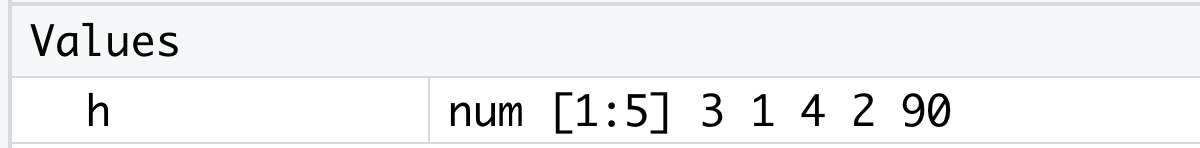
\includegraphics[width=0.7\linewidth]{pics/2h1} 

}

\caption{Values of h (1)}\label{fig:h1}
\end{figure}

We should agree that \texttt{h} is a numeric vector with 5 values Then let's try to do an object assignment again, this time you can assign different values to \texttt{h} and see what will happen to \texttt{h}.

\begin{Shaded}
\begin{Highlighting}[]
\NormalTok{h }\OtherTok{\textless{}{-}} \FunctionTok{c}\NormalTok{(}\DecValTok{1}\NormalTok{,}\DecValTok{2}\NormalTok{,}\DecValTok{3}\NormalTok{,}\DecValTok{4}\NormalTok{,}\DecValTok{5}\NormalTok{)}
\NormalTok{h}
\CommentTok{\#\textgreater{} [1] 1 2 3 4 5}
\end{Highlighting}
\end{Shaded}

Then you can see that the values of \texttt{h} have been changed to the new ones! Another easier way to verify values of \texttt{h} is from the environment, so it is a good habit to monitor the environment from time to time to make sure everything looks fine.

\begin{figure}

{\centering 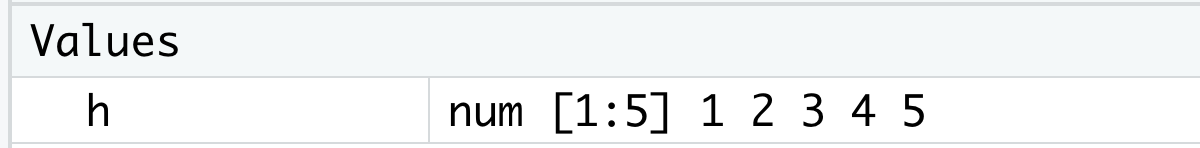
\includegraphics[width=0.7\linewidth]{pics/2h2} 

}

\caption{Values of h (2)}\label{fig:h2}
\end{figure}

You can assign any values to \texttt{h} as you want, then \texttt{h} may change the vector type or even the object type according to the values assigned. By running the following code, \texttt{h} will be a character vector with three strings.

\begin{Shaded}
\begin{Highlighting}[]
\NormalTok{h }\OtherTok{\textless{}{-}} \FunctionTok{c}\NormalTok{(}\StringTok{"pig"}\NormalTok{, }\StringTok{"monkey"}\NormalTok{, }\StringTok{"panda"}\NormalTok{)}
\end{Highlighting}
\end{Shaded}

\begin{figure}

{\centering 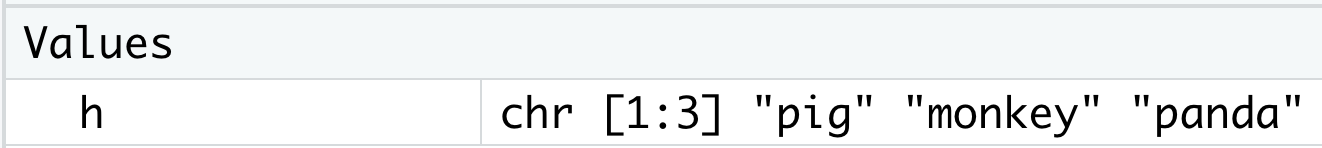
\includegraphics[width=0.7\linewidth]{pics/2h3} 

}

\caption{Values of h (3)}\label{fig:h3}
\end{figure}

\begin{infobox}{caution}

If you assign values of a subvector to a name, you will create a new vector. Now \texttt{hs} is not the subset of \texttt{h}, it is a vector with the same value as the subset. If you assign different value(s) to \texttt{hs}, there will be no change on \texttt{h}.

\begin{Shaded}
\begin{Highlighting}[]
\NormalTok{h }\OtherTok{\textless{}{-}} \FunctionTok{c}\NormalTok{(}\DecValTok{3}\NormalTok{,}\DecValTok{1}\NormalTok{,}\DecValTok{4}\NormalTok{,}\DecValTok{2}\NormalTok{,}\DecValTok{90}\NormalTok{)}
\NormalTok{hs }\OtherTok{\textless{}{-}}\NormalTok{ h[}\FunctionTok{c}\NormalTok{(}\DecValTok{2}\NormalTok{,}\DecValTok{4}\NormalTok{)]}
\NormalTok{hs }\OtherTok{\textless{}{-}} \DecValTok{10}
\NormalTok{h}
\end{Highlighting}
\end{Shaded}

\end{infobox}

\hypertarget{exercises-7}{%
\subsection{Exercises}\label{exercises-7}}

Consider the vector \texttt{v1\ \textless{}-\ c(7,\ 2,\ 4,\ 9,\ 7)}, \texttt{v2\ \textless{}-\ c(6,\ 2,\ 8,\ 7,\ 9)}, and \texttt{v3\ \textless{}-\ 1:50}.

\begin{enumerate}
\def\labelenumi{\arabic{enumi}.}
\item
  Find the locations in \texttt{v1} where the corresponding value is smaller than \texttt{v2}.
\item
  Find the subvector of \texttt{v2} such that the corresponding location in \texttt{v1} is larger than 5.
\item
  Find the subvector of \texttt{v3} such that it is divisible by 7. (Hint: the result of \texttt{7\%\%7} is equal to 0 since 7 is divisible by 7)
\item
  For all elements of \texttt{v3} that is divisible by 8, replace it by 100.
\end{enumerate}

\hypertarget{patterned_numeric_vectors_creation}{%
\section{Numeric Vectors: Creating numeric vectors with patterns}\label{patterned_numeric_vectors_creation}}

In Section \ref{intro-num-vector}, you learned how to create numeric vectors with length more than 1 by using the \texttt{c()} function. When the number of elements become too big, you may feel redundant manually typing in all those elements. Luckily, as long as the assigned elements have certain patterns, R allows you to create the desired numeric vector numeric vectors more efficiently.

\hypertarget{the-colon-operator-equally-spaced-numeric-vectors-with-increment-of-1-or--1}{%
\subsection{\texorpdfstring{The colon operator \texttt{:} -- Equally-spaced numeric vectors with increment of 1 or -1}{The colon operator : -- Equally-spaced numeric vectors with increment of 1 or -1}}\label{the-colon-operator-equally-spaced-numeric-vectors-with-increment-of-1-or--1}}

An equally-spaced numeric vector is a numeric vector with the same distance between adjacent elements. Suppose you want to assign consecutive integers from 1 to 5 to the name pattern1. Coming from Section \ref{intro-num-vector}, you may do the following:

\begin{Shaded}
\begin{Highlighting}[]
\NormalTok{pattern1 }\OtherTok{\textless{}{-}} \FunctionTok{c}\NormalTok{(}\DecValTok{1}\NormalTok{, }\DecValTok{2}\NormalTok{, }\DecValTok{3}\NormalTok{, }\DecValTok{4}\NormalTok{, }\DecValTok{5}\NormalTok{)}
\end{Highlighting}
\end{Shaded}

However, when the number of elements changes from 5 consecutive integers to 100 consecutive integers, manually typing in would be really time-consuming and inefficient. In R, you can use the colon operator \texttt{:} to create equally-spaced numeric vectors. Note that you don't need to use \texttt{:} together with \texttt{c()}.

\begin{Shaded}
\begin{Highlighting}[]
\NormalTok{pattern2 }\OtherTok{\textless{}{-}} \DecValTok{1}\SpecialCharTok{:}\DecValTok{5}
\end{Highlighting}
\end{Shaded}

If you compare \texttt{pattern1} and \texttt{pattern2}, you will realize that they are both numeric vectors with elements of consecutive integers from 1 to 5. Let's experiement \texttt{:} with more attempts.

\begin{Shaded}
\begin{Highlighting}[]
\NormalTok{pattern3 }\OtherTok{\textless{}{-}} \DecValTok{1}\SpecialCharTok{:}\DecValTok{100}
\NormalTok{pattern3}
\CommentTok{\#\textgreater{}   [1]   1   2   3   4   5   6   7   8   9  10  11  12  13  14  15  16  17  18}
\CommentTok{\#\textgreater{}  [19]  19  20  21  22  23  24  25  26  27  28  29  30  31  32  33  34  35  36}
\CommentTok{\#\textgreater{}  [37]  37  38  39  40  41  42  43  44  45  46  47  48  49  50  51  52  53  54}
\CommentTok{\#\textgreater{}  [55]  55  56  57  58  59  60  61  62  63  64  65  66  67  68  69  70  71  72}
\CommentTok{\#\textgreater{}  [73]  73  74  75  76  77  78  79  80  81  82  83  84  85  86  87  88  89  90}
\CommentTok{\#\textgreater{}  [91]  91  92  93  94  95  96  97  98  99 100}
\NormalTok{pattern4 }\OtherTok{\textless{}{-}} \DecValTok{5}\SpecialCharTok{:}\DecValTok{1}
\NormalTok{pattern4}
\CommentTok{\#\textgreater{} [1] 5 4 3 2 1}
\NormalTok{pattern5 }\OtherTok{\textless{}{-}} \FloatTok{1.2}\SpecialCharTok{:}\FloatTok{5.2}
\NormalTok{pattern5}
\CommentTok{\#\textgreater{} [1] 1.2 2.2 3.2 4.2 5.2}
\end{Highlighting}
\end{Shaded}

With \texttt{pattern3}, you can see how powerful and convenient the colon operator is. In addition to create ascending equally-spaced numeric vectors, you can also use it to create descending ones, like \texttt{pattern4}. Eventually, you can use the colon operator to assign equally-spaced decimals to numeric vectors.

However, as you can see below, R will store numeric vectors with equally-spaced integers as \textbf{type integer} and those with equally-spaced decimals as \textbf{type double}.

\begin{Shaded}
\begin{Highlighting}[]
\FunctionTok{class}\NormalTok{(pattern4)}
\CommentTok{\#\textgreater{} [1] "integer"}
\FunctionTok{class}\NormalTok{(pattern5)}
\CommentTok{\#\textgreater{} [1] "numeric"}
\end{Highlighting}
\end{Shaded}

\hypertarget{the-seq-function-equally-spaced-numeric-vectors-with-any-increment}{%
\subsection{\texorpdfstring{The \texttt{seq()} function -- Equally-spaced numeric vectors with any increment}{The seq() function -- Equally-spaced numeric vectors with any increment}}\label{the-seq-function-equally-spaced-numeric-vectors-with-any-increment}}

As powerful as the colon operator \texttt{:} is, it is really restricted to creating equally-spaced numeric vectors with an increment 1 or -1. By contrast, the \texttt{seq()} function don't have such a restriction, and it will come into play when you want to create equally-spaced numeric vectors with increments other than 1 or -1.

***a. Create sequences with the \texttt{by} argument

The \texttt{seq()} function can include three arguments: \texttt{from}, \texttt{to}, and \texttt{by}. The \texttt{from} and \texttt{to} arguments specify the start and limited end values, respectively, while the \texttt{by} argument specifies the increment of the sequence.

\begin{Shaded}
\begin{Highlighting}[]
\FunctionTok{seq}\NormalTok{(}\AttributeTok{from =} \DecValTok{1}\NormalTok{, }\AttributeTok{to =} \DecValTok{5}\NormalTok{, }\AttributeTok{by =} \DecValTok{1}\NormalTok{)}
\CommentTok{\#\textgreater{} [1] 1 2 3 4 5}
\FunctionTok{seq}\NormalTok{(}\AttributeTok{to =} \DecValTok{5}\NormalTok{)}
\CommentTok{\#\textgreater{} [1] 1 2 3 4 5}
\end{Highlighting}
\end{Shaded}

You can interpret the above example as ``an equally-spaced numeric vector starting at 1 and ending at 5, with the increment between adjacent elements of 1''. If you don't specify the optional \texttt{from} and \texttt{by} arguments, \texttt{seq()} will use the default value 1 for both arguments.

\begin{infobox}{caution}

Now you have had four methods to create vectors with consecutive integers.

\begin{Shaded}
\begin{Highlighting}[]
\FunctionTok{c}\NormalTok{(}\DecValTok{1}\NormalTok{,}\DecValTok{2}\NormalTok{,}\DecValTok{3}\NormalTok{,}\DecValTok{4}\NormalTok{,}\DecValTok{5}\NormalTok{,}\DecValTok{6}\NormalTok{)                }\CommentTok{\#write all numbers down}
\DecValTok{1}\SpecialCharTok{:}\DecValTok{6}                           \CommentTok{\#use colon operator}
\FunctionTok{seq}\NormalTok{(}\AttributeTok{from =} \DecValTok{1}\NormalTok{, }\AttributeTok{to =} \DecValTok{6}\NormalTok{, }\AttributeTok{by =} \DecValTok{1}\NormalTok{) }\CommentTok{\#use seq()}
\FunctionTok{seq}\NormalTok{(}\AttributeTok{to =} \DecValTok{6}\NormalTok{)                   }\CommentTok{\#use seq()}
\end{Highlighting}
\end{Shaded}

\end{infobox}

Next, let's assign a different value to the \texttt{by} argument in the \texttt{seq()} function. What you will get a numeric vector with \texttt{1\ 3\ 5} as its values.

\begin{Shaded}
\begin{Highlighting}[]
\FunctionTok{seq}\NormalTok{(}\AttributeTok{from =} \DecValTok{1}\NormalTok{, }\AttributeTok{to =} \DecValTok{5}\NormalTok{, }\AttributeTok{by =} \DecValTok{2}\NormalTok{)}
\CommentTok{\#\textgreater{} [1] 1 3 5}
\end{Highlighting}
\end{Shaded}

Note that the ending value of the sequence doesn't always equal the value assigned to the \texttt{to} argument. If you change the limit end value to 6, you still get the same sequence. This is because the next value in the sequence would be 7, which is larger than the limit end value 6. This is the reason why \texttt{to} denotes the limited end value, not the end value.

\begin{Shaded}
\begin{Highlighting}[]
\FunctionTok{seq}\NormalTok{(}\AttributeTok{from =} \DecValTok{1}\NormalTok{, }\AttributeTok{to =} \DecValTok{6}\NormalTok{, }\AttributeTok{by =} \DecValTok{2}\NormalTok{)}
\CommentTok{\#\textgreater{} [1] 1 3 5}
\end{Highlighting}
\end{Shaded}

Of course, you can assign decimal numbers to arguments in the \texttt{seq()} function. Below, you will first get a sequence which starts with 1, increases by 0.5 each time until it is larger than 6. Subsequently, you will get a numeric vector with \texttt{1.1\ 1.8\ 2.5\ 3.2} as its values.

\begin{Shaded}
\begin{Highlighting}[]
\FunctionTok{seq}\NormalTok{(}\AttributeTok{from =} \DecValTok{1}\NormalTok{, }\AttributeTok{to =} \DecValTok{6}\NormalTok{, }\AttributeTok{by =} \FloatTok{0.5}\NormalTok{) }
\CommentTok{\#\textgreater{}  [1] 1.0 1.5 2.0 2.5 3.0 3.5 4.0 4.5 5.0 5.5 6.0}
\FunctionTok{seq}\NormalTok{(}\AttributeTok{from =} \FloatTok{1.1}\NormalTok{, }\AttributeTok{to =} \FloatTok{3.2}\NormalTok{, }\AttributeTok{by =} \FloatTok{0.7}\NormalTok{) }
\CommentTok{\#\textgreater{} [1] 1.1 1.8 2.5 3.2}
\end{Highlighting}
\end{Shaded}

Besides ascending sequences, you can also create descending sequences via \texttt{seq()}. Similarly, you can assign positive numbers as well as negative ones to arguments in the \texttt{seq()} function. Try out some examples like below:

\begin{Shaded}
\begin{Highlighting}[]
\FunctionTok{seq}\NormalTok{(}\AttributeTok{from =} \FloatTok{1.5}\NormalTok{, }\AttributeTok{to =} \SpecialCharTok{{-}}\DecValTok{1}\NormalTok{, }\AttributeTok{by =} \SpecialCharTok{{-}}\FloatTok{0.5}\NormalTok{) }
\CommentTok{\#\textgreater{} [1]  1.5  1.0  0.5  0.0 {-}0.5 {-}1.0}
\FunctionTok{seq}\NormalTok{(}\AttributeTok{from =} \SpecialCharTok{{-}}\FloatTok{3.5}\NormalTok{, }\AttributeTok{to =} \SpecialCharTok{{-}}\DecValTok{3}\NormalTok{, }\AttributeTok{by =} \FloatTok{0.1}\NormalTok{)}
\CommentTok{\#\textgreater{} [1] {-}3.5 {-}3.4 {-}3.3 {-}3.2 {-}3.1 {-}3.0}
\FunctionTok{seq}\NormalTok{(}\AttributeTok{from =} \FloatTok{1.5}\NormalTok{, }\AttributeTok{to =} \SpecialCharTok{{-}}\DecValTok{1}\NormalTok{, }\AttributeTok{by =} \FloatTok{0.5}\NormalTok{) }
\CommentTok{\#\textgreater{} Error in seq.default(from = 1.5, to = {-}1, by = 0.5): wrong sign in \textquotesingle{}by\textquotesingle{} argument}
\end{Highlighting}
\end{Shaded}

It's worth-noting that the arguments in \texttt{seq()} function should make algebraic sense. For example, in the last example above, it doesn't make sense to use a positive value in the \texttt{by}argument when the start value is bigger than the limited end value, which implies a decreasing sequence. In such cases, You should expect to see an error message.

***b. Create sequences with the \texttt{length.out} argument

In \texttt{seq()}, instead of setting the increment via the \texttt{by} argument, you can also specify the \texttt{length.out} argument, which creates a equally-spaced sequence with the assigned length (a.k.a. the number of elements in the numeric vector). R will automatically calculate the difference between two neighboring elements according to values of three arguments in \texttt{seq()}.

\begin{Shaded}
\begin{Highlighting}[]
\FunctionTok{seq}\NormalTok{(}\AttributeTok{from =} \DecValTok{1}\NormalTok{, }\AttributeTok{to =} \DecValTok{5}\NormalTok{, }\AttributeTok{length.out =} \DecValTok{9}\NormalTok{) }
\CommentTok{\#\textgreater{} [1] 1.0 1.5 2.0 2.5 3.0 3.5 4.0 4.5 5.0}
\end{Highlighting}
\end{Shaded}

Here, you will get an equally-spaced sequence of length 9 from 1 to 5. You can also create a decreasing sequence by using the \texttt{length.out} argument.

\begin{Shaded}
\begin{Highlighting}[]
\FunctionTok{seq}\NormalTok{(}\AttributeTok{from =} \DecValTok{5}\NormalTok{, }\AttributeTok{to =} \SpecialCharTok{{-}}\DecValTok{5}\NormalTok{, }\AttributeTok{length.out =} \DecValTok{9}\NormalTok{) }
\CommentTok{\#\textgreater{} [1]  5.00  3.75  2.50  1.25  0.00 {-}1.25 {-}2.50 {-}3.75 {-}5.00}
\FunctionTok{seq}\NormalTok{(}\AttributeTok{from =} \DecValTok{5}\NormalTok{, }\AttributeTok{to =} \SpecialCharTok{{-}}\DecValTok{5}\NormalTok{, }\AttributeTok{length.out =} \FloatTok{8.9}\NormalTok{) }
\CommentTok{\#\textgreater{} [1]  5.00  3.75  2.50  1.25  0.00 {-}1.25 {-}2.50 {-}3.75 {-}5.00}
\end{Highlighting}
\end{Shaded}

What will happen if you assign a decimal number to the \texttt{length.out} argument? In such a case, R will round up the decimal to the nearest integer when carrying out the \texttt{length.out} argument. In the last example above, the value \texttt{8.9} is rounded up to \texttt{9}.

\begin{infobox}{caution}
Unlike creating sequences with \texttt{by} argument, if you specify the \texttt{length.out} argument in \texttt{seq()}, the start value and limited end value of the sequence you get will be exactly match the input arguments.

\end{infobox}

***c.~Create sequences with both the \texttt{by} and \texttt{length.out} arguments

Lastly, if you provide both the \texttt{by} and \texttt{length.out} arguments, only one of the \texttt{from} and \texttt{to} arguments is necessary. With one value (the start value or the limit end value) fixed, seq() will create a vector with specified increment and length.

If you only have the \texttt{from} argument, you will get a sequence starting from the value you set, with the increment in the \texttt{by} argument, until you get a sequence with a length specified in the \texttt{length.out} argument.

If you only have the \texttt{to} argument, you will get a sequence ending with the value you set, with the increment in the \texttt{by} argument, until you get a sequence with a length specified in the \texttt{length.out} argument.

\begin{Shaded}
\begin{Highlighting}[]
\FunctionTok{seq}\NormalTok{(}\AttributeTok{from =} \DecValTok{1}\NormalTok{, }\AttributeTok{by =} \DecValTok{2}\NormalTok{, }\AttributeTok{length.out =} \DecValTok{5}\NormalTok{)}
\CommentTok{\#\textgreater{} [1] 1 3 5 7 9}
\FunctionTok{seq}\NormalTok{(}\AttributeTok{to =} \DecValTok{1}\NormalTok{, }\AttributeTok{by =} \DecValTok{2}\NormalTok{, }\AttributeTok{length.out =} \DecValTok{5}\NormalTok{)}
\CommentTok{\#\textgreater{} [1] {-}7 {-}5 {-}3 {-}1  1}
\end{Highlighting}
\end{Shaded}

Before leaving the \texttt{seq()} function, you should be aware that you can \textbf{at most} provide three arguments. For example, you will see an error when running the following example since all four arguments are specified.

\begin{Shaded}
\begin{Highlighting}[]
\FunctionTok{seq}\NormalTok{(}\AttributeTok{from =} \DecValTok{1}\NormalTok{, }\AttributeTok{to =} \DecValTok{3}\NormalTok{, }\AttributeTok{by =} \DecValTok{1}\NormalTok{, }\AttributeTok{length.out =} \DecValTok{3}\NormalTok{)}
\CommentTok{\#\textgreater{} Error in seq.default(from = 1, to = 3, by = 1, length.out = 3): too many arguments}
\end{Highlighting}
\end{Shaded}

\hypertarget{the-sequence-generator-seq_along-matching-numeric-vectors}{%
\subsection{\texorpdfstring{The sequence generator \texttt{seq\_along()} -- Matching numeric vectors}{The sequence generator seq\_along() -- Matching numeric vectors}}\label{the-sequence-generator-seq_along-matching-numeric-vectors}}

Now, we will introduce one function derived from the \texttt{seq()} function. Let's first create a numeric vector \texttt{extend}.

\begin{Shaded}
\begin{Highlighting}[]
\NormalTok{extend }\OtherTok{\textless{}{-}} \FunctionTok{seq}\NormalTok{(}\AttributeTok{from =} \DecValTok{2}\NormalTok{, }\AttributeTok{to =} \DecValTok{8}\NormalTok{, }\AttributeTok{length.out =} \DecValTok{7}\NormalTok{) }
\NormalTok{extend}
\CommentTok{\#\textgreater{} [1] 2 3 4 5 6 7 8}
\end{Highlighting}
\end{Shaded}

By the value assigned to the \texttt{length.out} argument, you know that the length of \texttt{extend} is 7. You also know that \texttt{2\ 3\ 4\ 5\ 6\ 7\ 8} are the elements of \texttt{extend}. Next, let's put \texttt{extend} in \texttt{seq\_along()}.

\begin{Shaded}
\begin{Highlighting}[]
\FunctionTok{seq\_along}\NormalTok{(extend)}
\CommentTok{\#\textgreater{} [1] 1 2 3 4 5 6 7}
\end{Highlighting}
\end{Shaded}

As you can tell from the result, \texttt{seq\_along()} takes a numeric vector as its argument, generating consecutive integers from 1 to the length of the input vector. The \texttt{seq\_along()} function is commonly used when writing loops, which will be covered at a later time.

\begin{infobox}{caution}

You can also use \texttt{1:length(extend)} to get the same result as \texttt{seq\_along(extend)}.

\begin{Shaded}
\begin{Highlighting}[]
\DecValTok{1}\SpecialCharTok{:}\FunctionTok{length}\NormalTok{(extend)}
\CommentTok{\#\textgreater{} [1] 1 2 3 4 5 6 7}
\end{Highlighting}
\end{Shaded}

\end{infobox}

\hypertarget{the-rep-function-numeric-vectors-with-repeated-values}{%
\subsection{\texorpdfstring{The \texttt{rep()} Function -- Numeric vectors with repeated values}{The rep() Function -- Numeric vectors with repeated values}}\label{the-rep-function-numeric-vectors-with-repeated-values}}

The \texttt{rep()} function is designed for another type of patterned numeric vectors, which are with replicated values as their elements. To do repetition, you can use the \texttt{rep()} function, which works by repeating the first argument for the number of times indicated in the second argument. Suppose you want to assign four 2s to the name num1. You can use the \texttt{rep()} function here:

\begin{Shaded}
\begin{Highlighting}[]
\NormalTok{num1 }\OtherTok{\textless{}{-}} \FunctionTok{rep}\NormalTok{(}\DecValTok{2}\NormalTok{, }\DecValTok{4}\NormalTok{)}
\NormalTok{num1}
\CommentTok{\#\textgreater{} [1] 2 2 2 2}
\end{Highlighting}
\end{Shaded}

You can interpret the function as ``creating a numeric vector in which 2 is repeated four times''. The resulting vector is a length-4 numeric vector with all elements of value 2. In addition to one single value, a numeric vector with several values can be assigned in the first argument.

\begin{Shaded}
\begin{Highlighting}[]
\NormalTok{num2 }\OtherTok{\textless{}{-}} \FunctionTok{rep}\NormalTok{(}\FunctionTok{c}\NormalTok{(}\DecValTok{1}\NormalTok{, }\DecValTok{4}\NormalTok{, }\DecValTok{2}\NormalTok{), }\DecValTok{3}\NormalTok{)}
\NormalTok{num2}
\CommentTok{\#\textgreater{} [1] 1 4 2 1 4 2 1 4 2}
\end{Highlighting}
\end{Shaded}

Here, the \texttt{rep()} will repeat the whole vector c(1, 4, 2) three times. Note that the vector is \textbf{repeated as a whole}, not elementwisely. Reflectively, you may be wondering what happens the second argument also has several numbers? Let's try together.

\begin{Shaded}
\begin{Highlighting}[]
\NormalTok{num3 }\OtherTok{\textless{}{-}} \FunctionTok{rep}\NormalTok{(}\FunctionTok{c}\NormalTok{(}\DecValTok{1}\NormalTok{,}\DecValTok{5}\NormalTok{,}\DecValTok{7}\NormalTok{), }\FunctionTok{c}\NormalTok{(}\DecValTok{3}\NormalTok{,}\DecValTok{2}\NormalTok{,}\DecValTok{1}\NormalTok{))}
\NormalTok{num3}
\CommentTok{\#\textgreater{} [1] 1 1 1 5 5 7}
\end{Highlighting}
\end{Shaded}

In \texttt{rep()}, when the second argument is also a numeric vector, R will do an element-repeat-operation by repeating each element in the first argument the number of times indicated in the corresponding index of the second argument and combine the repeated vectors to a single numeric vector. In this example, 1 is repeated 3 times, 4 is repeated twice, and 7 is repeated once. It is equivalent to

\begin{Shaded}
\begin{Highlighting}[]
\FunctionTok{c}\NormalTok{(}\FunctionTok{rep}\NormalTok{(}\DecValTok{1}\NormalTok{,}\DecValTok{3}\NormalTok{), }\FunctionTok{rep}\NormalTok{(}\DecValTok{4}\NormalTok{,}\DecValTok{2}\NormalTok{), }\FunctionTok{rep}\NormalTok{(}\DecValTok{7}\NormalTok{,}\DecValTok{1}\NormalTok{))}
\CommentTok{\#\textgreater{} [1] 1 1 1 4 4 7}
\end{Highlighting}
\end{Shaded}

It is important that, to assign two numeric vectors as the two arguments in \texttt{rep()}, the two numeric vectors should have the same length. Otherwise, you will see an error message telling you the second argument (a.k.a. the \texttt{times} argument) is invalid.

\begin{Shaded}
\begin{Highlighting}[]
\NormalTok{num4 }\OtherTok{\textless{}{-}} \FunctionTok{rep}\NormalTok{(}\FunctionTok{c}\NormalTok{(}\DecValTok{1}\NormalTok{,}\DecValTok{5}\NormalTok{,}\DecValTok{7}\NormalTok{), }\FunctionTok{c}\NormalTok{(}\DecValTok{3}\NormalTok{,}\DecValTok{2}\NormalTok{))}
\CommentTok{\#\textgreater{} Error in rep(c(1, 5, 7), c(3, 2)): invalid \textquotesingle{}times\textquotesingle{} argument}
\end{Highlighting}
\end{Shaded}

\hypertarget{the-unique-and-table-functions-getting-unique-elements-and-their-frequencies}{%
\subsection{\texorpdfstring{The \texttt{unique()} and \texttt{table()} Functions -- Getting unique elements and their frequencies}{The unique() and table() Functions -- Getting unique elements and their frequencies}}\label{the-unique-and-table-functions-getting-unique-elements-and-their-frequencies}}

So far, you have learned how to create vectors with specific patterns. Sometimes, you may want to inspect the unique elements (elements with different values) in a numeric vector and their corresponding frequencies. Let's use num3 as an example. \textbf{(Don't forget to use ls() or check the environment panel to find all objects you have defined)},

\begin{Shaded}
\begin{Highlighting}[]
\NormalTok{num3}
\CommentTok{\#\textgreater{} [1] 1 1 1 5 5 7}
\end{Highlighting}
\end{Shaded}

You can use \texttt{unique()} to show all unique elements in vectors.

\begin{Shaded}
\begin{Highlighting}[]
\FunctionTok{unique}\NormalTok{(num3)}
\CommentTok{\#\textgreater{} [1] 1 5 7}
\end{Highlighting}
\end{Shaded}

From the result, you know the unique elements in \texttt{num3} are \texttt{1}, \texttt{5}, and \texttt{7}. To get the frequency of each element, you can use the \texttt{table()} function.

\begin{Shaded}
\begin{Highlighting}[]
\FunctionTok{table}\NormalTok{(num3)}
\CommentTok{\#\textgreater{} num3}
\CommentTok{\#\textgreater{} 1 5 7 }
\CommentTok{\#\textgreater{} 3 2 1}
\end{Highlighting}
\end{Shaded}

Here, the first row is the numeric vector's name. The second row shows all unique elements, and the third row is their corresponding frequencies. In num3, there are three 1s, two 5s and one 7.

\hypertarget{exercises-8}{%
\subsection{Exercises}\label{exercises-8}}

\begin{enumerate}
\def\labelenumi{\arabic{enumi}.}
\item
  Use five different ways to create an equally-spaced sequence with \texttt{2\ 4\ 6\ 8\ 10} as result.
\item
  Use two different ways to create a numeric vector with \texttt{1\ 2\ 3\ 1\ 2\ 3\ 4\ 5\ 1\ 2\ 3\ 4\ 5\ 6\ 7} as result. Show the unique elements and their corresponding frequency.
\end{enumerate}

\hypertarget{numeric-sort-rank-order}{%
\section{Numeric Vectors: Sort, Rank, Order}\label{numeric-sort-rank-order}}

After creating a numeric vector, we usually need to arrange (sort) the elements in either ascending or descending order. In this section, we will introduce how to sort numeric vectors and two other measures related to sorting.

First, let's create a numeric vector to be used throughout this section.

\begin{Shaded}
\begin{Highlighting}[]
\NormalTok{x }\OtherTok{\textless{}{-}} \FunctionTok{c}\NormalTok{(}\DecValTok{2}\NormalTok{, }\DecValTok{3}\NormalTok{, }\DecValTok{2}\NormalTok{, }\DecValTok{0}\NormalTok{, }\DecValTok{4}\NormalTok{, }\DecValTok{7}\NormalTok{) }
\NormalTok{x }\CommentTok{\#check the value of x}
\CommentTok{\#\textgreater{} [1] 2 3 2 0 4 7}
\end{Highlighting}
\end{Shaded}

\hypertarget{sort-vectors-with-sort}{%
\subsection{\texorpdfstring{Sort vectors with \texttt{sort()}}{Sort vectors with sort()}}\label{sort-vectors-with-sort}}

The first function we will introduce is \texttt{sort()}. By default, the \texttt{sort()} function \textbf{sort} elements in vector in the \textbf{ascending} order, namely from the smallest to largest.

\begin{Shaded}
\begin{Highlighting}[]
\FunctionTok{sort}\NormalTok{(x)}
\CommentTok{\#\textgreater{} [1] 0 2 2 3 4 7}
\end{Highlighting}
\end{Shaded}

If you want to sort the vector in the \textbf{descending} order, namely from the largest to smallest, you can add a second argument \texttt{decreasing\ =\ TRUE}.

\begin{Shaded}
\begin{Highlighting}[]
\FunctionTok{sort}\NormalTok{(x, }\AttributeTok{decreasing =} \ConstantTok{TRUE}\NormalTok{)}
\CommentTok{\#\textgreater{} [1] 7 4 3 2 2 0}
\end{Highlighting}
\end{Shaded}

\hypertarget{get-ranks-in-vectors-with-rank}{%
\subsection{\texorpdfstring{Get ranks in vectors with \texttt{rank()}}{Get ranks in vectors with rank()}}\label{get-ranks-in-vectors-with-rank}}

Next, let's talk about ranks in a vector. The \texttt{rank()} function gives the \textbf{ranks} for each element of the vector, namely the corresponding positions in the \textbf{ascending order}. It is worth mentioning that, in R, indexes start at 1 - the 1st element of is at index 1, and the following indexes will count as normal.

\begin{Shaded}
\begin{Highlighting}[]
\FunctionTok{rank}\NormalTok{(x)}
\CommentTok{\#\textgreater{} [1] 2.5 4.0 2.5 1.0 5.0 6.0}
\end{Highlighting}
\end{Shaded}

If you check the values of \texttt{x}, you can see that the smallest value of \texttt{x} is 0, which corresponds to the element at the fourth position of the original \texttt{x} vector. Thus, a rank of 1 will be assigned to the fourth position of the rank vector.

The second smallest value of \texttt{x} is 2, which appears twice at the first and the third positions, resulting a \textbf{tie} (elements with the same value will result in a tie). Normally, these two elements would have ranks 2 and 3, respectively. To break the tie, the \texttt{rank()} function assigns the \textbf{average} of the ranks for all elements within a tie situation, by default. For our example, the average of 2 and 3 is 2.5, and will be assigned to the first and the third position of the rank vector. In addition to this default behavior for handling ties, \texttt{rank()} also provides other options by setting the \texttt{ties.method} argument.

The third smallest value of \texttt{x} is 3, with a rank of 4 at the second position, thus a 4.0 will appear at the second position in the rank vector. The rest of the ranks is assigned in the same fashion.

If you set \texttt{ties.method\ =\ "min"}, all the tied elements will have the \emph{minimum rank} instead of the average rank. In this case, the minimum rank is 2.

\begin{Shaded}
\begin{Highlighting}[]
\FunctionTok{rank}\NormalTok{(x, }\AttributeTok{ties.method =} \StringTok{"min"}\NormalTok{)}
\CommentTok{\#\textgreater{} [1] 2 4 2 1 5 6}
\end{Highlighting}
\end{Shaded}

If you want to break the ties by the locations of the tied elements appear in the vector, you can set \texttt{ties.method\ =\ "first"}. Then, the earlier-appearing elements will have smaller ranks than the later-appearing ones. In this example, the first element will have rank 2 and the third element has rank 3, since the first element appears earlier than the third element. There are other options for handling ties, which you can look up in the documentation of \texttt{rank()} if interested.

\begin{Shaded}
\begin{Highlighting}[]
\FunctionTok{rank}\NormalTok{(x, }\AttributeTok{ties.method =} \StringTok{"first"}\NormalTok{)}
\CommentTok{\#\textgreater{} [1] 2 4 3 1 5 6}
\end{Highlighting}
\end{Shaded}

\begin{infobox}{caution}

Unlike \texttt{sort()}, you can't get positions in the descending order from the \texttt{rank()} function by adding \texttt{decreasing\ =\ TRUE} in \texttt{rank()}. However, you can achieve this goal by using \texttt{sort(-x)} if you want to get the positions in the descending order for vector \texttt{x}.

\begin{Shaded}
\begin{Highlighting}[]
\FunctionTok{sort}\NormalTok{(}\SpecialCharTok{{-}}\NormalTok{x)}
\CommentTok{\#\textgreater{} [1] {-}7 {-}4 {-}3 {-}2 {-}2  0}
\end{Highlighting}
\end{Shaded}

\end{infobox}

\hypertarget{get-the-ordering-permutation-via-order}{%
\subsection{Get the ordering permutation via `order()}\label{get-the-ordering-permutation-via-order}}

The next item we want to introduce is the \texttt{order()} function. Note that the function name \textbf{order} could be a bit misleading since ordering elements also has the same meaning of sorting. However, although it is related to sorting, \texttt{order()} is a very \emph{different} function from \texttt{sort()}.

Let's recall the values of \texttt{x} and apply \texttt{order()} on \texttt{x}.

\begin{Shaded}
\begin{Highlighting}[]
\NormalTok{x}
\CommentTok{\#\textgreater{} [1] 2 3 2 0 4 7}
\FunctionTok{order}\NormalTok{(x)}
\CommentTok{\#\textgreater{} [1] 4 1 3 2 5 6}
\FunctionTok{sort}\NormalTok{(x)}
\CommentTok{\#\textgreater{} [1] 0 2 2 3 4 7}
\end{Highlighting}
\end{Shaded}

From the result, you can see that the \texttt{order()} function returns \textbf{indices} for the elements in the \textbf{ascending} order, namely from the smallest to the largest. For example, the first output is 4, since the 4th element in \texttt{x} is the smallest. The second output is 1, since the 1st element in \texttt{x} is the second smallest. In other words, \texttt{order()} returns a \textbf{permutation} which rearranges the vector \texttt{x} into ascending order, which is shown in the following example.

\begin{Shaded}
\begin{Highlighting}[]
\NormalTok{x[}\FunctionTok{order}\NormalTok{(x)]}
\CommentTok{\#\textgreater{} [1] 0 2 2 3 4 7}
\end{Highlighting}
\end{Shaded}

\begin{infobox}{caution}
Unlike \texttt{rank()}, the \texttt{order()} function breaks the ties by the appearing order by default.

\end{infobox}

If you want the indices corresponding to the descending order, then you can set \texttt{decreasing\ =\ TRUE} just like what we did in the \texttt{sort()} function.

\begin{Shaded}
\begin{Highlighting}[]
\FunctionTok{order}\NormalTok{(x, }\AttributeTok{decreasing =} \ConstantTok{TRUE}\NormalTok{)  }
\CommentTok{\#\textgreater{} [1] 6 5 2 1 3 4}
\end{Highlighting}
\end{Shaded}

In this section, we have covered \texttt{sort()}, \texttt{rank()}, and \texttt{order()} functions for numeric vectors. It is helpful to provide a brief summary.

\begin{itemize}
\tightlist
\item
  The \texttt{sort()} function sorts elements in vectors in ascending/descending order.
\item
  The \texttt{rank()} function produces ranks for each element of the vector.
\item
  The \texttt{order()} function returns the corresponding indices in ascending/descending order for the elements.
\end{itemize}

\hypertarget{exercises-9}{%
\subsection{Exercises}\label{exercises-9}}

Write R codes to solve the following problems.

\begin{enumerate}
\def\labelenumi{\arabic{enumi}.}
\item
  Create a numeric vector named \texttt{exe} with values \texttt{2,\ 0,\ -3,\ 0,\ 5,\ 6} and sort \texttt{exe} from the largest to the smallest.
\item
  In \texttt{exe}, what's the ranks of \texttt{2} and the first \texttt{0}?
\item
  For \texttt{exe}, get indices for the elements in the ascending order.
\end{enumerate}

\hypertarget{numeric-vector-statistics}{%
\section{Numeric vector: Summary Statistics}\label{numeric-vector-statistics}}

We've spent several sections learning the features of numeric vectors. In this section, we will introduce statistical functions on numeric vectors.

Let's first create a numeric vector.

\begin{Shaded}
\begin{Highlighting}[]
\NormalTok{h }\OtherTok{\textless{}{-}} \FunctionTok{c}\NormalTok{(}\DecValTok{3}\NormalTok{, }\DecValTok{2}\NormalTok{, }\DecValTok{75}\NormalTok{, }\DecValTok{0}\NormalTok{, }\DecValTok{100}\NormalTok{)}
\NormalTok{h }\CommentTok{\#check the value of h}
\CommentTok{\#\textgreater{} [1]   3   2  75   0 100}
\end{Highlighting}
\end{Shaded}

Next, we will divide statistical functions into several groups, and introduce them one by one.

\hypertarget{minimum-and-maximum}{%
\subsection{Minimum and Maximum}\label{minimum-and-maximum}}

\begin{Shaded}
\begin{Highlighting}[]
\FunctionTok{min}\NormalTok{(h) }
\CommentTok{\#\textgreater{} [1] 0}
\FunctionTok{max}\NormalTok{(h) }
\CommentTok{\#\textgreater{} [1] 100}
\FunctionTok{range}\NormalTok{(h)}
\CommentTok{\#\textgreater{} [1]   0 100}
\end{Highlighting}
\end{Shaded}

First, you can get the \textbf{minimum} and \textbf{maximum} values of a numeric vector by calling the \texttt{min()} and \texttt{max()} functions, respectively. To get these two values at one time, you can call the \texttt{range()} function, which returns a length-2 vector with the minimum value(the first element) and maximum value(the second element).

\begin{Shaded}
\begin{Highlighting}[]
\FunctionTok{which.min}\NormalTok{(h) }
\CommentTok{\#\textgreater{} [1] 4}
\FunctionTok{which.max}\NormalTok{(h) }
\CommentTok{\#\textgreater{} [1] 5}
\end{Highlighting}
\end{Shaded}

In addition to getting the minimum and the maximum values, it is often useful to get the corresponding locations of them. In \texttt{h}, the minimum value 0 is located in the fourth place, and this is why you will get a result of \texttt{4} from \texttt{which.min()}. If multiple elements are assigned with the same minimum value, \texttt{which.min()} will return the first location. Similarly, \texttt{which.max()} tells you the location of the maximum value.

\begin{infobox}{caution}

\begin{Shaded}
\begin{Highlighting}[]
\NormalTok{g }\OtherTok{\textless{}{-}} \FunctionTok{c}\NormalTok{(}\DecValTok{2}\NormalTok{, }\DecValTok{2}\NormalTok{, }\DecValTok{1}\NormalTok{, }\DecValTok{1}\NormalTok{)}
\FunctionTok{which.min}\NormalTok{(g)}
\CommentTok{\#\textgreater{} [1] 3}
\FunctionTok{which.max}\NormalTok{(g)}
\CommentTok{\#\textgreater{} [1] 1}
\end{Highlighting}
\end{Shaded}

The third and fourth elements in \texttt{g} both have the minimum value, but \texttt{which.min(g)} returns a result of 3 since the minimum value firstly appears in the third element. Similarly, \texttt{which.max()} gives you a result of \texttt{1}.

\end{infobox}

\begin{Shaded}
\begin{Highlighting}[]
\FunctionTok{cummin}\NormalTok{(h) }
\CommentTok{\#\textgreater{} [1] 3 2 2 0 0}
\FunctionTok{cummax}\NormalTok{(h) }
\CommentTok{\#\textgreater{} [1]   3   3  75  75 100}
\end{Highlighting}
\end{Shaded}

In addition to calculating the minimum value of all elements, you can also use the \textbf{cumulative minimum} function, called \texttt{cummin()}. It returns a vector of the same length as the input vector, with the value at each location being the minimum of all preceding elements until that location in the original vector. For example, the first element of \texttt{cummin(h)} is \texttt{3} because the minimum of the first element in the original vector is always itself. The second element of \texttt{cummin(h)} is \texttt{2}, since the minimum of the first two elements (\texttt{3} and \texttt{2}) in \texttt{h}is 2, and so on.

Note that once we reach the minimum value of the original vector, the remaining elements of the cumulative minimum function will always equal to the minimum value. There is also a corresponding function for computing the cumulative maximums, called \texttt{cummax()}.

\hypertarget{sum-and-product}{%
\subsection{Sum and Product}\label{sum-and-product}}

\begin{Shaded}
\begin{Highlighting}[]
\FunctionTok{sum}\NormalTok{(h)}
\CommentTok{\#\textgreater{} [1] 180}
\FunctionTok{cumsum}\NormalTok{(h)}
\CommentTok{\#\textgreater{} [1]   3   5  80  80 180}
\end{Highlighting}
\end{Shaded}

Next, let's look at the \texttt{sum()} function, which produces the \textbf{sum} of all elements in the vector. For the numeric vector \texttt{h}, the sum is \texttt{3+2+75+0+100}, which is \texttt{180}. Similar to \texttt{cummin()}, you can use the \texttt{cumsum()} function to compute the \emph{cumulative sums}, which works by summing up the elements of the original vector cumulatively up to each location. In \texttt{cumsum(h)}, the first element is \texttt{3} since there is only one element (\texttt{3}) to do summation, and the second element is \texttt{5} since the summation of the first two elements (\texttt{3} and \texttt{2}) in \texttt{h} is 5. You can easily verify the values of the remaining elements by yourself.

\begin{Shaded}
\begin{Highlighting}[]
\FunctionTok{prod}\NormalTok{(h)}
\CommentTok{\#\textgreater{} [1] 0}
\FunctionTok{cumprod}\NormalTok{(h)}
\CommentTok{\#\textgreater{} [1]   3   6 450   0   0}
\end{Highlighting}
\end{Shaded}

As long as we can calculate the sum and cumulative sum of a numeric vector, we can also compute the \textbf{product} of a numeric vector's elements by the \texttt{prod()} function. In \texttt{h}, since there is \texttt{0} in \texttt{h}, the result is \texttt{0}. Similarly, we have the \emph{cumulative product} function \texttt{cumprod()} working by multiplying the elements of the original vector cumulatively up to each location.

\begin{Shaded}
\begin{Highlighting}[]
\NormalTok{h}
\CommentTok{\#\textgreater{} [1]   3   2  75   0 100}
\FunctionTok{diff}\NormalTok{(h)}
\CommentTok{\#\textgreater{} [1]  {-}1  73 {-}75 100}
\end{Highlighting}
\end{Shaded}

\#我就是好奇查了一下diff() functions,下面这一段可以是optional的,但是it is worth noting that diff() 和 sum() 的mechanism不一样
It is worth noting that the \texttt{diff()} function doesn't work the same way as the \texttt{sum()} function. Specifically, \texttt{diff()} returns the \textbf{difference between consecutive elements} in a numeric vector. In \texttt{h}, the difference between the first and the second elements (\texttt{3} and \texttt{2}) is \texttt{-1}, whereas that between the second and the third elements (\texttt{2} and \texttt{75}) is \texttt{73}. In other words, the computations in done by subtracting the former element from the latter one in a consecutive pair.

\hypertarget{mean-and-median}{%
\subsection{Mean and median}\label{mean-and-median}}

\begin{Shaded}
\begin{Highlighting}[]
\FunctionTok{mean}\NormalTok{(h)}
\CommentTok{\#\textgreater{} [1] 36}
\FunctionTok{median}\NormalTok{(h)}
\CommentTok{\#\textgreater{} [1] 3}
\end{Highlighting}
\end{Shaded}

The \textbf{arithmetic mean} of a numeric vector's elements can be easily computed via the \texttt{mean()} function. To get the median of a numeric vector's elements, we would need to place them in value order and find the middle. The \texttt{sort()} function introduced previously can list elements in order from the smallest to the largest. Comparatively, the \texttt{median()} function first places the elements in value order and then returns the middle number.

If the vector length is odd, the middle number is the value of the element in the central location. In \texttt{sort(h)}, we can see that the median corresponds to the third number out of five numbers since there are two numbers larger than 3 and two numbers smaller than 3. If the vector length is even, the middle number is the average of the two middle elements after sorting.

\begin{infobox}{caution}

\begin{Shaded}
\begin{Highlighting}[]
\FunctionTok{sort}\NormalTok{(g)}
\CommentTok{\#\textgreater{} [1] 1 1 2 2}
\FunctionTok{median}\NormalTok{(g)}
\CommentTok{\#\textgreater{} [1] 1.5}
\end{Highlighting}
\end{Shaded}

Recall \texttt{g} with values of \texttt{2}, \texttt{2}, \texttt{1}, \texttt{1}. After sorting, you will see that \texttt{1} and \texttt{2} are in the middle. The median is then defined as the average of these two elements, namely 1.5.

\end{infobox}

\hypertarget{quantiles}{%
\subsection{Quantiles}\label{quantiles}}

\begin{Shaded}
\begin{Highlighting}[]
\FunctionTok{quantile}\NormalTok{(h)}
\CommentTok{\#\textgreater{}   0\%  25\%  50\%  75\% 100\% }
\CommentTok{\#\textgreater{}    0    2    3   75  100}
\end{Highlighting}
\end{Shaded}

\texttt{quantile()} produces \textbf{sample quantiles} of a given numeric vector. By default, it generates 2 rows and 5 numbers. The top row represents the different percentiles, which are always the 0 percentile, 25th percentile (0.25 quantile), 50th percentile (0.5 quantile), 75th percentile (0.75 quantile), and 100th percentile. The second row consists of the corresponding values of each quantile. We next go over all five quantile values.

First of all, 0 percentile and 100th percentile are always the minimum and the maximum values, respectively. The 50th percentile (0.5 quantile) is the same as the median.

The 25-th percentile (0.25 quantile), also called the \textbf{first quartile}, is the value such that there are 25 percent (or a quarter) of the remaining data (all elements without this number) smaller than it. For vector \texttt{h}, the value is 2 since there is exactly 1 number, which is 25 percent of the remaining 4 numbers, smaller than 2.

Similarly, the 75-th percentile, also called the \textbf{third quartile}, is the value such that 75 percent of the remaining data is smaller than this number. For vector \texttt{h}, the value is 75 since there are 3 numbers, which are 75 percent of the remaining 4 numbers, smaller than 75.

You also have an important concept called \textbf{interquartile range} (IQR), defined as the difference between the 3rd quartile (75-th percentile) and the 1st quartile (25-th percentile). The interquartile range of \texttt{h} is 73, which is \texttt{75\ -\ 2}.

\begin{Shaded}
\begin{Highlighting}[]
\FunctionTok{IQR}\NormalTok{(h)}
\CommentTok{\#\textgreater{} [1] 73}
\end{Highlighting}
\end{Shaded}

In addition to the default five percentiles, the \texttt{quantile()} function can also compute a specific quantile between 0 and 1. To do this, you just need to specify the second argument \texttt{probs}. Let's try to find the 95th quantile.

\begin{Shaded}
\begin{Highlighting}[]
\FunctionTok{quantile}\NormalTok{(h, }\AttributeTok{probs =} \FloatTok{0.95}\NormalTok{)}
\CommentTok{\#\textgreater{} 95\% }
\CommentTok{\#\textgreater{}  95}
\end{Highlighting}
\end{Shaded}

As before, this asks R to compute the 95th percentile, meaning 95 percent of the remaining data is smaller than this value. Because you only have 5 values in this vector, it may not be very intuitive. However, if you have more elements in a vector, say 1001, you can count the number of the remaining data that is smaller than this value, which should be 950 (the number of remaining data is 1000, and 95 percent of 1000 is 950).

In addition, the second argument can be a vector of probabilities, which will produce a numeric vector of the corresponding quantiles.

\begin{Shaded}
\begin{Highlighting}[]
\FunctionTok{quantile}\NormalTok{(h, }\AttributeTok{probs =} \FunctionTok{c}\NormalTok{(}\FloatTok{0.1}\NormalTok{, }\FloatTok{0.2}\NormalTok{, }\FloatTok{0.99}\NormalTok{))}
\CommentTok{\#\textgreater{}  10\%  20\%  99\% }
\CommentTok{\#\textgreater{}  0.8  1.6 99.0}
\end{Highlighting}
\end{Shaded}

\hypertarget{summary-statistics}{%
\subsection{Summary statistics}\label{summary-statistics}}

\begin{Shaded}
\begin{Highlighting}[]
\FunctionTok{summary}\NormalTok{(h)}
\CommentTok{\#\textgreater{}    Min. 1st Qu.  Median    Mean 3rd Qu.    Max. }
\CommentTok{\#\textgreater{}       0       2       3      36      75     100}
\end{Highlighting}
\end{Shaded}

Compared with \texttt{quantile()}, the \texttt{summary} function produces a more comprehensive picture of a numeric vector. Applying \texttt{summary()}, you can get the 5 percentiles and the arithmetic mean at one time.\\
(Min: 0 percentile, 1st Qu: 25-th percentile, Median: 50-th percentile, 3rd Qu: 75-th percentile, Max: 100-th percentile)

\textbf{\emph{Group F: variance and standard deviation}}

\begin{Shaded}
\begin{Highlighting}[]
\FunctionTok{var}\NormalTok{(h)}
\CommentTok{\#\textgreater{} [1] 2289.5}
\FunctionTok{sd}\NormalTok{(h)}
\CommentTok{\#\textgreater{} [1] 47.84872}
\end{Highlighting}
\end{Shaded}

The last group of functions are \texttt{var()} and \texttt{sd()}, which compute the \textbf{sample variance} and \textbf{sample standard deviation} of a numeric vector, respectively. The formula of sample variance of vector \(h\) is \[var(h) = \frac{1}{n-1}\sum_{i=1}^n (h_i-\bar h)^2,\] where \(n\) is the length of \(h\) and \(\bar h\) is the average of all elements. By definition, the sample standard deviation is the square root of sample variance, which you can verify by \texttt{sqrt(var(h))}.

For your convenience, we would like to provide a summary of all the functions introduced in the following table.

\begin{tabular}{l|l|l}
\hline
Operation & Explanation & Length\\
\hline
min(h) & the minimum value & 1\\
\hline
max(h) & the maximum value & 1\\
\hline
range(h) & both the minimum value and the maximum value & 2\\
\hline
which.min(h) & the (first) location of the minimum value & 1\\
\hline
which.max(h) & the (first) location of the maximum value & 1\\
\hline
cummin(h) & the cumulative minimum values & same as the original numeric vector\\
\hline
cummax(h) & the cumulative maximum values & same as the original numeric vector\\
\hline
sum(h) & the sum of all elements & 1\\
\hline
cumsum(h) & the cumulative sum & same as the original numeric vector\\
\hline
prod(h) & the product of all elements & 1\\
\hline
cumprod(h) & the cumulative products & same as the original numeric vector\\
\hline
mean(h) & the average of all elements & 1\\
\hline
median(h) & the middle number in sort(h) & 1\\
\hline
quantile(h) & the 0 percentile, 25-th percentile, 50-th percentile, 75-th percentile, and 100-th percentile & 5\\
\hline
IQR(h) & the difference between the 3rd quartile and the 1st quartile & 1\\
\hline
quantile(h, probs = 0.95) & the 95-th percentile & 1\\
\hline
quantile(h, probs = c(0.1, 0.2, 0.99)) & several quantiles at a time & same as the argument numeric vector\\
\hline
summary(h) & 5 percentiles and the mean & 6\\
\hline
var(h) & the sample variance & 1\\
\hline
sd(h) & the sample standard deviation & 1\\
\hline
\end{tabular}

\hypertarget{exercises-10}{%
\subsection{Exercises}\label{exercises-10}}

Suppose \texttt{x\ \textless{}-\ c(5,\ 2,\ 4,\ 1,\ 2,\ 1)}

\begin{enumerate}
\def\labelenumi{\arabic{enumi}.}
\item
  Write the R code to reproduce each element of the summary vector \texttt{summary(x)}
\item
  Write the R code to generate the cumulative sum, cumulative product, cumulative minimum, and cumulative maximum of \texttt{x}.
\item
  Write R code to generate a vector consisting of the 0.1, 0.2, 0.6, 0.8, 0.9 quantiles of \texttt{x}.
\item
  Write R code to calculate the sample variance and sample standard deviation of \texttt{x}.
\end{enumerate}

\hypertarget{char-concatenate}{%
\section{Character Vectors: Create with Repetition and Concatenate}\label{char-concatenate}}

From this section, we will dive deep into \textbf{character vectors}.

\hypertarget{create-character-vectors-with-repetition}{%
\subsection{Create character vectors with repetition}\label{create-character-vectors-with-repetition}}

Just like numeric vectors, you can also create character vectors with \textbf{repetition} via the \texttt{rep()} function.

\begin{Shaded}
\begin{Highlighting}[]
\FunctionTok{rep}\NormalTok{(}\StringTok{"sheep"}\NormalTok{, }\DecValTok{5}\NormalTok{)}
\CommentTok{\#\textgreater{} [1] "sheep" "sheep" "sheep" "sheep" "sheep"}
\end{Highlighting}
\end{Shaded}

If the first argument is of length larger than 1, and the second argument is a single integer, the \texttt{rep()} function will \textbf{repeat} the first vector the corresponding times that is specified by the integer.

\begin{Shaded}
\begin{Highlighting}[]
\FunctionTok{rep}\NormalTok{(}\FunctionTok{c}\NormalTok{(}\StringTok{"sheep"}\NormalTok{, }\StringTok{"monkey"}\NormalTok{), }\DecValTok{3}\NormalTok{)}
\CommentTok{\#\textgreater{} [1] "sheep"  "monkey" "sheep"  "monkey" "sheep"  "monkey"}
\end{Highlighting}
\end{Shaded}

Another option is to specify the second argument as a numeric vector of the same length as the vector to be repeated. In this case, each element of the character vector will be sequentially repeated the corresponding number of times. Please see the following examples.

\begin{Shaded}
\begin{Highlighting}[]
\FunctionTok{rep}\NormalTok{(}\FunctionTok{c}\NormalTok{(}\StringTok{"sheep"}\NormalTok{, }\StringTok{"monkey"}\NormalTok{), }\FunctionTok{rep}\NormalTok{(}\DecValTok{3}\NormalTok{, }\DecValTok{2}\NormalTok{))}
\CommentTok{\#\textgreater{} [1] "sheep"  "sheep"  "sheep"  "monkey" "monkey" "monkey"}
\FunctionTok{rep}\NormalTok{(}\FunctionTok{c}\NormalTok{(}\StringTok{"sheep"}\NormalTok{, }\StringTok{"monkey"}\NormalTok{), }\FunctionTok{c}\NormalTok{(}\DecValTok{3}\NormalTok{,}\DecValTok{4}\NormalTok{))}
\CommentTok{\#\textgreater{} [1] "sheep"  "sheep"  "sheep"  "monkey" "monkey" "monkey" "monkey"}
\end{Highlighting}
\end{Shaded}

\hypertarget{concatenate-strings-with-paste}{%
\subsection{\texorpdfstring{Concatenate strings with \texttt{paste()}}{Concatenate strings with paste()}}\label{concatenate-strings-with-paste}}

Next, we will introduce how to \textbf{concatenate} several strings into a single string. To do this, you can use the \texttt{paste()} function. First, let's create a character vector with four elements,

\begin{Shaded}
\begin{Highlighting}[]
\NormalTok{four\_strings }\OtherTok{\textless{}{-}} \FunctionTok{c}\NormalTok{(}\StringTok{"I"}\NormalTok{, }\StringTok{"love"}\NormalTok{, }\StringTok{"r02pro"}\NormalTok{, }\StringTok{"!"}\NormalTok{)}
\NormalTok{four\_strings}
\CommentTok{\#\textgreater{} [1] "I"      "love"   "r02pro" "!"}
\FunctionTok{length}\NormalTok{(four\_strings) }\CommentTok{\#verify the number of strings}
\CommentTok{\#\textgreater{} [1] 4}
\end{Highlighting}
\end{Shaded}

To concatenate the four strings in to a single string, you can use \texttt{paste()} instead of \texttt{c()}:

\begin{Shaded}
\begin{Highlighting}[]
\NormalTok{one\_long\_string }\OtherTok{\textless{}{-}} \FunctionTok{paste}\NormalTok{(}\StringTok{"I"}\NormalTok{, }\StringTok{"love"}\NormalTok{, }\StringTok{"r02pro"}\NormalTok{, }\StringTok{"!"}\NormalTok{)}
\NormalTok{one\_long\_string}
\CommentTok{\#\textgreater{} [1] "I love r02pro !"}
\end{Highlighting}
\end{Shaded}

You can verify the class and length of the new object.

\begin{Shaded}
\begin{Highlighting}[]
\FunctionTok{class}\NormalTok{(one\_long\_string)}
\CommentTok{\#\textgreater{} [1] "character"}
\FunctionTok{length}\NormalTok{(one\_long\_string) }\CommentTok{\#verify the number of strings}
\CommentTok{\#\textgreater{} [1] 1}
\end{Highlighting}
\end{Shaded}

From the results, you can see that \texttt{one\_long\_string} is a character vector with length 1, and the value of \texttt{one\_long\_string} is a single string with spaces between the individual strings.

In \texttt{paste()}, the default \textbf{separator} between the individual strings is space. Take a look at the documentation of the \texttt{paste()} function with any form of getting help (Section \ref{Calculator}) that we previously introduced. What does the \texttt{sep\ =\ "\ "} argument mean? In fact, you can change the separator by setting the \texttt{sep} argument as a string in \texttt{paste()}. For example, you can separate the individual strings with comma or \texttt{!\&!}.

\begin{Shaded}
\begin{Highlighting}[]
\NormalTok{comma }\OtherTok{\textless{}{-}} \FunctionTok{paste}\NormalTok{(}\StringTok{"I"}\NormalTok{, }\StringTok{"love"}\NormalTok{, }\StringTok{"r02pro"}\NormalTok{, }\StringTok{"!"}\NormalTok{, }\AttributeTok{sep =} \StringTok{","}\NormalTok{) }
\NormalTok{comma}
\CommentTok{\#\textgreater{} [1] "I,love,r02pro,!"}
\FunctionTok{paste}\NormalTok{(}\StringTok{"I"}\NormalTok{, }\StringTok{"love"}\NormalTok{, }\StringTok{"r02pro"}\NormalTok{, }\StringTok{"!"}\NormalTok{, }\AttributeTok{sep =} \StringTok{"!\&!"}\NormalTok{) }
\CommentTok{\#\textgreater{} [1] "I!\&!love!\&!r02pro!\&!!"}
\end{Highlighting}
\end{Shaded}

If you don't want to use a separator, you can set \texttt{sep\ =\ ""} or use the \texttt{paste0()} function.

\begin{Shaded}
\begin{Highlighting}[]
\FunctionTok{paste}\NormalTok{(}\StringTok{"I"}\NormalTok{, }\StringTok{"love"}\NormalTok{, }\StringTok{"r02pro"}\NormalTok{, }\StringTok{"!"}\NormalTok{, }\AttributeTok{sep =} \StringTok{""}\NormalTok{)}
\CommentTok{\#\textgreater{} [1] "Ilover02pro!"}
\FunctionTok{paste0}\NormalTok{(}\StringTok{"I"}\NormalTok{, }\StringTok{"love"}\NormalTok{, }\StringTok{"r02pro"}\NormalTok{, }\StringTok{"!"}\NormalTok{) }
\CommentTok{\#\textgreater{} [1] "Ilover02pro!"}
\end{Highlighting}
\end{Shaded}

You may noticed the next argument for \texttt{paste()} is \texttt{collapse\ =\ NULL} in the documentation. If you would like to concatenate the elements of a vector into a longer string, you need to specify the \texttt{collapse} argument as the separator instead of \texttt{sep} in the \texttt{paste()} function.

\begin{Shaded}
\begin{Highlighting}[]
\FunctionTok{paste}\NormalTok{(four\_strings, }\AttributeTok{collapse =} \StringTok{""}\NormalTok{)}
\CommentTok{\#\textgreater{} [1] "Ilover02pro!"}
\FunctionTok{paste}\NormalTok{(four\_strings, }\AttributeTok{collapse =} \StringTok{","}\NormalTok{)}
\CommentTok{\#\textgreater{} [1] "I,love,r02pro,!"}
\FunctionTok{paste}\NormalTok{(four\_strings)                 }\DocumentationTok{\#\#doesn\textquotesingle{}t work without the collapse argument}
\CommentTok{\#\textgreater{} [1] "I"      "love"   "r02pro" "!"}
\end{Highlighting}
\end{Shaded}

In addition to paste several strings into one long string, you can also use the \texttt{paste()} function to concatenate two or more character vectors, where the pair of strings will be pasted elementwisely.

\begin{Shaded}
\begin{Highlighting}[]
\FunctionTok{paste}\NormalTok{(}\FunctionTok{c}\NormalTok{(}\StringTok{"July"}\NormalTok{, }\StringTok{"August"}\NormalTok{),  }\FunctionTok{c}\NormalTok{(}\StringTok{"2007"}\NormalTok{, }\StringTok{"2008"}\NormalTok{))}
\CommentTok{\#\textgreater{} [1] "July 2007"   "August 2008"}
\end{Highlighting}
\end{Shaded}

Note that you can take advantage of the \textbf{recycling rule} by using single strings in the character vectors.

\begin{Shaded}
\begin{Highlighting}[]
\FunctionTok{paste}\NormalTok{(}\StringTok{"Do"}\NormalTok{, }\FunctionTok{c}\NormalTok{(}\StringTok{"I"}\NormalTok{, }\StringTok{"you"}\NormalTok{, }\StringTok{"they"}\NormalTok{), }\StringTok{"love r02pro?"}\NormalTok{)}
\CommentTok{\#\textgreater{} [1] "Do I love r02pro?"    "Do you love r02pro?"  "Do they love r02pro?"}
\FunctionTok{paste}\NormalTok{(}\StringTok{"Yes!"}\NormalTok{, }\FunctionTok{c}\NormalTok{(}\StringTok{"I"}\NormalTok{, }\StringTok{"You"}\NormalTok{, }\StringTok{"They"}\NormalTok{), }\StringTok{"love r02pro!"}\NormalTok{)}
\CommentTok{\#\textgreater{} [1] "Yes! I love r02pro!"    "Yes! You love r02pro!"  "Yes! They love r02pro!"}
\end{Highlighting}
\end{Shaded}

By default, the arguments in the \texttt{paste()} function are all character vectors. However, if you mix vectors of different types, all elements will be converted to characters based on the coercion rule (Section \ref{coercion-rule}) before being concatenated.

\begin{Shaded}
\begin{Highlighting}[]
\FunctionTok{paste}\NormalTok{(}\FunctionTok{c}\NormalTok{(}\StringTok{"Peter"}\NormalTok{, }\StringTok{"James"}\NormalTok{, }\StringTok{"Mary"}\NormalTok{), }\StringTok{"has been learning R for"}\NormalTok{, }\DecValTok{2}\SpecialCharTok{:}\DecValTok{4}\NormalTok{, }\StringTok{"years."}\NormalTok{)}
\CommentTok{\#\textgreater{} [1] "Peter has been learning R for 2 years."}
\CommentTok{\#\textgreater{} [2] "James has been learning R for 3 years."}
\CommentTok{\#\textgreater{} [3] "Mary has been learning R for 4 years."}
\FunctionTok{paste}\NormalTok{(}\StringTok{"The statement is"}\NormalTok{, }\FunctionTok{c}\NormalTok{(T, F))}
\CommentTok{\#\textgreater{} [1] "The statement is TRUE"  "The statement is FALSE"}
\end{Highlighting}
\end{Shaded}

\hypertarget{output-via-cat}{%
\subsection{\texorpdfstring{Output via \texttt{cat()}}{Output via cat()}}\label{output-via-cat}}

Another commonly used function related to character vectors is the \texttt{cat()} function, which converts its arguments to character vectors, concatenates them to a single character vector, appends the given \textbf{separator} specified in the optional argument \texttt{sep} to each element, and then outputs them. The default separator is space.

\begin{Shaded}
\begin{Highlighting}[]
\FunctionTok{cat}\NormalTok{(}\StringTok{"I"}\NormalTok{, }\StringTok{"am"}\NormalTok{, }\StringTok{"a"}\NormalTok{, }\StringTok{"long"}\NormalTok{, }\StringTok{"string"}\NormalTok{)}
\CommentTok{\#\textgreater{} I am a long string}
\end{Highlighting}
\end{Shaded}

Let's try to specify the separator \texttt{sep\ =\ "\$"}.

\begin{Shaded}
\begin{Highlighting}[]
\FunctionTok{cat}\NormalTok{(}\StringTok{"I"}\NormalTok{, }\StringTok{"am"}\NormalTok{, }\StringTok{"a"}\NormalTok{, }\StringTok{"long"}\NormalTok{, }\StringTok{"string"}\NormalTok{, }\AttributeTok{sep =} \StringTok{"$"}\NormalTok{)}
\CommentTok{\#\textgreater{} I$am$a$long$string}
\end{Highlighting}
\end{Shaded}

The \texttt{cat()} function is super useful when one wants to print a message in user-defined functions. Some important characters are the \textbf{newline character} \texttt{\textbackslash{}n}, and the \textbf{tab character} \texttt{\textbackslash{}t}. Let's try it in action. Please pay special attention to the effects of \texttt{\textbackslash{}n} and \texttt{\textbackslash{}t} characters.

\begin{Shaded}
\begin{Highlighting}[]
\FunctionTok{cat}\NormalTok{(}\StringTok{"I"}\NormalTok{, }\StringTok{"am"}\NormalTok{, }\StringTok{"}\SpecialCharTok{\textbackslash{}n}\StringTok{"}\NormalTok{, }\StringTok{"starting }\SpecialCharTok{\textbackslash{}t}\StringTok{ line 2...."}\NormalTok{, }
    \StringTok{"a"}\NormalTok{, }\StringTok{"long"}\NormalTok{, }\StringTok{"}\SpecialCharTok{\textbackslash{}n}\StringTok{"}\NormalTok{, }\StringTok{"starting line 3...."}\NormalTok{, }\StringTok{"string"}\NormalTok{)}
\CommentTok{\#\textgreater{} I am }
\CommentTok{\#\textgreater{}  starting     line 2.... a long }
\CommentTok{\#\textgreater{}  starting line 3.... string}
\end{Highlighting}
\end{Shaded}

Similar to the \texttt{paste()} function, implicit coercion will also apply before the concatenate process.

\begin{Shaded}
\begin{Highlighting}[]
\FunctionTok{cat}\NormalTok{(}\FunctionTok{c}\NormalTok{(}\StringTok{"Peter"}\NormalTok{, }\StringTok{"James"}\NormalTok{, }\StringTok{"and Mary"}\NormalTok{),}\StringTok{"}\SpecialCharTok{\textbackslash{}n}\StringTok{"}\NormalTok{, }
    \StringTok{"have been learning R for}\SpecialCharTok{\textbackslash{}n}\StringTok{"}\NormalTok{, }\DecValTok{2}\SpecialCharTok{:}\DecValTok{4}\NormalTok{, }\StringTok{"years,}\SpecialCharTok{\textbackslash{}n}\StringTok{"}\NormalTok{,}
    \StringTok{"respectively."}\NormalTok{)}
\CommentTok{\#\textgreater{} Peter James and Mary }
\CommentTok{\#\textgreater{}  have been learning R for}
\CommentTok{\#\textgreater{}  2 3 4 years,}
\CommentTok{\#\textgreater{}  respectively.}
\end{Highlighting}
\end{Shaded}

\hypertarget{exercises-11}{%
\subsection{Exercises}\label{exercises-11}}

\begin{enumerate}
\def\labelenumi{\arabic{enumi}.}
\tightlist
\item
  Write R codes using the \texttt{rep()} function to reproduce the following three vectors with alphabetic letter values. Try not put direct letters in your code.
\end{enumerate}

i). a b c d a b c d a b c d
ii). a a a b b b c c c d d d
iii). a a a a b b b b c c d

\begin{enumerate}
\def\labelenumi{\arabic{enumi}.}
\setcounter{enumi}{1}
\tightlist
\item
  Please use the \texttt{paste()} function to reproduce the following sentences.
\end{enumerate}

Alice has been playing tennis for 4 years in London.
Bob has been playing soccer for 3 years in New York.
Charlie has been playing baseball for 2 years in Berlin.

\begin{enumerate}
\def\labelenumi{\arabic{enumi}.}
\setcounter{enumi}{2}
\tightlist
\item
  Please use the \texttt{paste()} and \texttt{cat()} functions to reproduce the following message.
\end{enumerate}

\begin{verbatim}
#> Starting i = 1
#>  Starting i = 2
#>  Starting i = 3
#>  Starting i = 4
#>  Starting i = 5
#>  Starting i = 6
#>  Starting i = 7
#>  Starting i = 8
#>  Starting i = 9
#>  Starting i = 10
\end{verbatim}

\hypertarget{character-sort-rank-order}{%
\section{Character Vectors: Sort, Rank, Order}\label{character-sort-rank-order}}

In Section \ref{numeric-sort-rank-order}, you learned \texttt{sort()}, \texttt{rank()\textasciigrave{}\textasciigrave{},\ and}order()` to sort numeric vectors and get their elements' ranks and indices. These three functions can be used in a similar manner for character vectors. Similar to numeric vectors, let's first prepare a character vector.

\begin{Shaded}
\begin{Highlighting}[]
\NormalTok{char\_vec }\OtherTok{\textless{}{-}} \FunctionTok{c}\NormalTok{(}\StringTok{"a"}\NormalTok{, }\StringTok{"A"}\NormalTok{, }\StringTok{"B"}\NormalTok{, }\StringTok{"b"}\NormalTok{, }\StringTok{"aB"}\NormalTok{,}\StringTok{"ac"}\NormalTok{, }\StringTok{"1c"}\NormalTok{, }\StringTok{".a"}\NormalTok{, }\StringTok{"1a"}\NormalTok{,}\StringTok{"2a"}\NormalTok{,}\StringTok{".a"}\NormalTok{,}\StringTok{"\&u"}\NormalTok{,}\StringTok{"3"}\NormalTok{,}\StringTok{"\_4"}\NormalTok{)}
\end{Highlighting}
\end{Shaded}

\hypertarget{ordering-rules}{%
\subsection{Ordering rules}\label{ordering-rules}}

For character vectors, R uses the \textbf{lexicographical ordering}, which is sometimes called dictionary order since it is the order used in a dictionary. Note that the strings in character vectors can contain letters, numbers, or symbols. There are a few important ordering rules as follows.

\begin{itemize}
\item
  symbols \textless{} digits \textless{} letters: symbols appear first, followed by digits, and letters appear last.
\item
  symbols are ordered in a specific way as shown below.
\end{itemize}

\begin{Shaded}
\begin{Highlighting}[]
\NormalTok{syms }\OtherTok{\textless{}{-}} \FunctionTok{c}\NormalTok{(}\StringTok{" "}\NormalTok{,}\StringTok{","}\NormalTok{,}\StringTok{";"}\NormalTok{,}\StringTok{"\_"}\NormalTok{,}\StringTok{"("}\NormalTok{,}\StringTok{")"}\NormalTok{,}\StringTok{"!"}\NormalTok{,}\StringTok{"["}\NormalTok{,}\StringTok{"]"}\NormalTok{,}\StringTok{"\{"}\NormalTok{,}\StringTok{"\}"}\NormalTok{,}\StringTok{"{-}"}\NormalTok{,}\StringTok{"*"}\NormalTok{,}\StringTok{"/"}\NormalTok{,}\StringTok{"\#"}\NormalTok{,}\StringTok{"$"}\NormalTok{,}\StringTok{"\%"}\NormalTok{,}\StringTok{"\^{}"}\NormalTok{,}\StringTok{"\&"}\NormalTok{,}\StringTok{"\textasciigrave{}"}\NormalTok{,}\StringTok{"@"}\NormalTok{,}\StringTok{"+"}\NormalTok{,}\StringTok{"="}\NormalTok{,}\StringTok{"|"}\NormalTok{,}\StringTok{"?"}\NormalTok{,}\StringTok{"\textless{}"}\NormalTok{,}\StringTok{"\textgreater{}"}\NormalTok{,}\StringTok{"."}\NormalTok{)}
\FunctionTok{sort}\NormalTok{(syms)}
\CommentTok{\#\textgreater{}  [1] " " "\_" "{-}" "," ";" "!" "?" "." "(" ")" "[" "]" "\{" "\}" "@" "*" "/" "\&" "\#"}
\CommentTok{\#\textgreater{} [20] "\%" "\textasciigrave{}" "\^{}" "+" "\textless{}" "=" "\textgreater{}" "|" "$"}
\end{Highlighting}
\end{Shaded}

\begin{itemize}
\tightlist
\item
  digits are ordered ascendingly: the smaller digits appear earlier than the bigger ones.
\end{itemize}

\begin{Shaded}
\begin{Highlighting}[]
\NormalTok{nums }\OtherTok{\textless{}{-}} \DecValTok{0}\SpecialCharTok{:}\DecValTok{9}
\FunctionTok{sort}\NormalTok{(nums)}
\CommentTok{\#\textgreater{}  [1] 0 1 2 3 4 5 6 7 8 9}
\end{Highlighting}
\end{Shaded}

\begin{itemize}
\tightlist
\item
  Letters have two sorting rules. In R, \texttt{letters} is a pre-created character vector with all 26 lower-cased letters in the alphabet, and \texttt{LETTERS} is another character vector with all 26 upper-cased letters in the alphabet. Case-wise, lower cases go before upper cases. Letter-wise, letters are sorted alphabetically.
\end{itemize}

\begin{Shaded}
\begin{Highlighting}[]
\NormalTok{all\_letters }\OtherTok{\textless{}{-}} \FunctionTok{c}\NormalTok{(letters,LETTERS)}
\FunctionTok{sort}\NormalTok{(all\_letters)}
\CommentTok{\#\textgreater{}  [1] "a" "A" "b" "B" "c" "C" "d" "D" "e" "E" "f" "F" "g" "G" "h" "H" "i" "I" "j"}
\CommentTok{\#\textgreater{} [20] "J" "k" "K" "l" "L" "m" "M" "n" "N" "o" "O" "p" "P" "q" "Q" "r" "R" "s" "S"}
\CommentTok{\#\textgreater{} [39] "t" "T" "u" "U" "v" "V" "w" "W" "x" "X" "y" "Y" "z" "Z"}
\end{Highlighting}
\end{Shaded}

From the example below, you will find out that the letter-wise rule always overweighs the case-wise rule. \#麻烦帮忙看看这里讲得清不清楚

\begin{Shaded}
\begin{Highlighting}[]
\NormalTok{x }\OtherTok{\textless{}{-}} \FunctionTok{c}\NormalTok{(}\StringTok{"d"}\NormalTok{, }\StringTok{"c"}\NormalTok{)}
\FunctionTok{sort}\NormalTok{(x)}
\CommentTok{\#\textgreater{} [1] "c" "d"}
\NormalTok{y }\OtherTok{\textless{}{-}} \FunctionTok{c}\NormalTok{(}\StringTok{"d"}\NormalTok{, }\StringTok{"C"}\NormalTok{)}
\FunctionTok{sort}\NormalTok{(y)}
\CommentTok{\#\textgreater{} [1] "C" "d"}
\end{Highlighting}
\end{Shaded}

\hypertarget{sort-vectors-with-sort-1}{%
\subsection{\texorpdfstring{Sort vectors with \texttt{sort()}}{Sort vectors with sort()}}\label{sort-vectors-with-sort-1}}

You can surely apply \texttt{sort()} on character vectors. A character vector's elements (i.e., strings) are sorted by their first character. If two elements have the same first character, they will be sorted by their second character. The rule applies until the indexed ties between two strings' characters are broken, or two strings run out of characters.

Let's try to sort the character vector \texttt{char\_vec}.

\begin{Shaded}
\begin{Highlighting}[]
\FunctionTok{sort}\NormalTok{(char\_vec)}
\CommentTok{\#\textgreater{}  [1] "\_4" ".a" ".a" "\&u" "1a" "1c" "2a" "3"  "a"  "A"  "aB" "ac" "b"  "B"}
\end{Highlighting}
\end{Shaded}

We have the following observations.

\begin{itemize}
\tightlist
\item
  Symbols appear first, followed by digits, and letters appear last.
\item
  According to the ordering rule of symbols, \texttt{\_4} goes first, \texttt{.a} (two of them) and \texttt{\&u} follow subsequently.
\item
  \texttt{1a} and \texttt{1c} have the same first character. Between their second character, a goes before c, therefore \texttt{1a} goes before \texttt{1c}.
\item
  \texttt{aB} and \texttt{ac} have the same first character, since b goes before C (although B is an upper case while c is a lower case), \texttt{aB} goes before \texttt{ac}.
\end{itemize}

Of course, we can also have the order reversed by adding the argument \texttt{decreasing\ =\ TRUE} inside \texttt{sort()}.

\begin{Shaded}
\begin{Highlighting}[]
\FunctionTok{sort}\NormalTok{(char\_vec, }\AttributeTok{decreasing =} \ConstantTok{TRUE}\NormalTok{)}
\CommentTok{\#\textgreater{}  [1] "B"  "b"  "ac" "aB" "A"  "a"  "3"  "2a" "1c" "1a" "\&u" ".a" ".a" "\_4"}
\end{Highlighting}
\end{Shaded}

\hypertarget{get-ranks-in-vectors-with-rank-1}{%
\subsection{\texorpdfstring{Get ranks in vectors with \texttt{rank()}}{Get ranks in vectors with rank()}}\label{get-ranks-in-vectors-with-rank-1}}

The same ordering rules introduced in subsection \ref{ordering-rules} do apply when R ranks a character vector's strings. Here, the element with rank 1 is \texttt{\_4} and \texttt{.a} has rank 2. Just like numeric vectors, if you have strings with the same value (i.e., characters) in character vectors, these elements' ranks will be the same (the average of the corresponding ranks) by default.

\begin{Shaded}
\begin{Highlighting}[]
\FunctionTok{rank}\NormalTok{(char\_vec)}
\CommentTok{\#\textgreater{}  [1]  9.0 10.0 14.0 13.0 11.0 12.0  6.0  2.5  5.0  7.0  2.5  4.0  8.0  1.0}
\end{Highlighting}
\end{Shaded}

As expected, you can set the \texttt{ties.method} argument in \texttt{rank()} to use other methods for breaking ties.

\begin{Shaded}
\begin{Highlighting}[]
\FunctionTok{rank}\NormalTok{(char\_vec, }\AttributeTok{ties.method =} \StringTok{"min"}\NormalTok{)}
\CommentTok{\#\textgreater{}  [1]  9 10 14 13 11 12  6  2  5  7  2  4  8  1}
\FunctionTok{rank}\NormalTok{(char\_vec, }\AttributeTok{ties.method =} \StringTok{"first"}\NormalTok{)}
\CommentTok{\#\textgreater{}  [1]  9 10 14 13 11 12  6  2  5  7  3  4  8  1}
\end{Highlighting}
\end{Shaded}

\hypertarget{get-the-ordering-permutation-via-order-1}{%
\subsection{\texorpdfstring{Get the ordering permutation via \texttt{order()}}{Get the ordering permutation via order()}}\label{get-the-ordering-permutation-via-order-1}}

Again, you can use the same \texttt{order()} function to get the corresponding indices of a character vector's strings. Also, the \texttt{order()} function breaks the ties by the appearing order by default.

\begin{Shaded}
\begin{Highlighting}[]
\FunctionTok{order}\NormalTok{(char\_vec)}
\CommentTok{\#\textgreater{}  [1] 14  8 11 12  9  7 10 13  1  2  5  6  4  3}
\end{Highlighting}
\end{Shaded}

The \texttt{decreasing} argument still works for \texttt{order()}:

\begin{Shaded}
\begin{Highlighting}[]
\FunctionTok{order}\NormalTok{(char\_vec, }\AttributeTok{decreasing =} \ConstantTok{TRUE}\NormalTok{)}
\CommentTok{\#\textgreater{}  [1]  3  4  6  5  2  1 13 10  7  9 12  8 11 14}
\end{Highlighting}
\end{Shaded}

\hypertarget{summary-and-comparisons}{%
\subsection{Summary and comparisons}\label{summary-and-comparisons}}

Let's put all sort-related functions together to clarify their functions.

\begin{Shaded}
\begin{Highlighting}[]
\NormalTok{char\_vec}
\CommentTok{\#\textgreater{}  [1] "a"  "A"  "B"  "b"  "aB" "ac" "1c" ".a" "1a" "2a" ".a" "\&u" "3"  "\_4"}
\end{Highlighting}
\end{Shaded}

\begin{Shaded}
\begin{Highlighting}[]
\FunctionTok{sort}\NormalTok{(char\_vec)}
\CommentTok{\#\textgreater{}  [1] "\_4" ".a" ".a" "\&u" "1a" "1c" "2a" "3"  "a"  "A"  "aB" "ac" "b"  "B"}
\end{Highlighting}
\end{Shaded}

The \texttt{sort()} function \textbf{sort} \texttt{char\_vec} according to previously introduced ordering rules. \texttt{\_4} goes first because its first character is a symbol (symbols \textless{} digits \textless{} letters), and \texttt{\_} goes before ``.'' and ``\&''.

\begin{Shaded}
\begin{Highlighting}[]
\FunctionTok{rank}\NormalTok{(char\_vec)}
\CommentTok{\#\textgreater{}  [1]  9.0 10.0 14.0 13.0 11.0 12.0  6.0  2.5  5.0  7.0  2.5  4.0  8.0  1.0}
\end{Highlighting}
\end{Shaded}

The \texttt{rank()} function gives the \textbf{ranks} of strings inside \texttt{char\_vec}. The first returned rank is \texttt{9.0} because the first string in \texttt{char\_vec}, namely ``a'', is sorted in the 9th place in \texttt{char\_vec}. The second returned rank is \texttt{10.0} because the second string in \texttt{char\_vec}, namely ``A'', is sorted in the 10th place in \texttt{char\_vec}.

\begin{Shaded}
\begin{Highlighting}[]
\FunctionTok{order}\NormalTok{(char\_vec)}
\CommentTok{\#\textgreater{}  [1] 14  8 11 12  9  7 10 13  1  2  5  6  4  3}
\end{Highlighting}
\end{Shaded}

The \texttt{order()} function gives the \textbf{ordering permutation} of \texttt{char\_vec}. The first returned order is 14 because sorting \texttt{char\_vec} will put this character vector's 14th string, namely "\_4``, in the first place. Similarly, the second returned order is 8 because sorting \texttt{char\_vec} will put this character vector's 8th string, namely''.a", in the second place.

\hypertarget{exercises-12}{%
\subsection{Exercises}\label{exercises-12}}

Suppose \texttt{exercise\ \textless{}-\ c("\&5",\ "Nd",\ "9iC",\ "3df",\ "df",\ "nd",\ "\_5",\ "9ic")}

\begin{enumerate}
\def\labelenumi{\arabic{enumi}.}
\item
  Sort \texttt{exercise} in the ascending order. Explain why 1) \texttt{3df} goes before \texttt{9ic}; 2) \texttt{\&5} goes before \texttt{3df}; 3) \texttt{9ic} goes before \texttt{9iC}.
\item
  Apply both \texttt{rank()} and \texttt{order()} to the character vector \texttt{exercise}. Within the two returned vectors, explain how does the element \texttt{7} means differently in two vectors.
\end{enumerate}

\hypertarget{factors}{%
\section{Character Vectors, Factors \& Ordered Factors}\label{factors}}

Having learned various aspects of character vectors, we will introduce a very important class of objects in this section, named \textbf{factors}. First, let's create a character vector to be used in this section.

\begin{Shaded}
\begin{Highlighting}[]
\NormalTok{animals }\OtherTok{\textless{}{-}} \FunctionTok{c}\NormalTok{(}\StringTok{"sheep"}\NormalTok{, }\StringTok{"pig"}\NormalTok{, }\StringTok{"monkey"}\NormalTok{, }\StringTok{"sheep"}\NormalTok{, }\StringTok{"sheep"}\NormalTok{, }\StringTok{"pig"}\NormalTok{)}
\end{Highlighting}
\end{Shaded}

\hypertarget{create-a-factor-from-a-vector}{%
\subsection{Create a factor from a vector}\label{create-a-factor-from-a-vector}}

So, what is exactly a \textbf{factor}? It can be viewed as a special type of vector whose elements take on a \textbf{fixed and known} set of different values. You can create a factor from a vector using the \texttt{factor()} function. To understand the output of a factor, it is helpful to compare the results with the original vector \texttt{animals}.

\begin{Shaded}
\begin{Highlighting}[]
\NormalTok{animals\_fac }\OtherTok{\textless{}{-}} \FunctionTok{factor}\NormalTok{(animals)  }
\NormalTok{animals\_fac}
\CommentTok{\#\textgreater{} [1] sheep  pig    monkey sheep  sheep  pig   }
\CommentTok{\#\textgreater{} Levels: monkey pig sheep}
\NormalTok{animals}
\CommentTok{\#\textgreater{} [1] "sheep"  "pig"    "monkey" "sheep"  "sheep"  "pig"}
\end{Highlighting}
\end{Shaded}

First, note that the strings in the character vector all have quotation marks around the elements, while the corresponding factor doesn't have them. Second, we see an additional row in the factor, starting with ``Levels:''. This shows the unique elements of \texttt{animals} ordered alphabetically.

If you use the \texttt{class()} function on \texttt{animals\_fac}, you will see it is indeed a factor.

\begin{Shaded}
\begin{Highlighting}[]
\FunctionTok{class}\NormalTok{(animals\_fac)}
\CommentTok{\#\textgreater{} [1] "factor"}
\FunctionTok{class}\NormalTok{(animals)}
\CommentTok{\#\textgreater{} [1] "character"}
\end{Highlighting}
\end{Shaded}

To retrieve the levels of a factor, you can use the function \texttt{levels()} on it.

\begin{Shaded}
\begin{Highlighting}[]
\FunctionTok{levels}\NormalTok{(animals\_fac)}
\CommentTok{\#\textgreater{} [1] "monkey" "pig"    "sheep"}
\end{Highlighting}
\end{Shaded}

To have a deeper understanding on factors, it is helpful to check its internal storage type using \texttt{typeof()}.

\begin{Shaded}
\begin{Highlighting}[]
\FunctionTok{typeof}\NormalTok{(animals\_fac)}
\CommentTok{\#\textgreater{} [1] "integer"}
\FunctionTok{as.numeric}\NormalTok{(animals\_fac)}
\CommentTok{\#\textgreater{} [1] 3 2 1 3 3 2}
\end{Highlighting}
\end{Shaded}

Perhaps a bit surprisingly, a factor is stored as integers. The integers represent the corresponding locations of each element in the levels. For example, the first value of \texttt{as.numeric(animals\_fac)} is 3, since the first element of \texttt{animals\_fac} is \texttt{"sheep"}, which is the third element in the levels. The particular storage mechanism for factors is very appealing in the sense that storing integers takes much less space than storing all the same levels repeatedly in the original character vector. As the same time, you can easily reproduce the original character vector using the integers and the factor levels using vector subsetting via indices.

\begin{Shaded}
\begin{Highlighting}[]
\FunctionTok{levels}\NormalTok{(animals\_fac)[}\FunctionTok{as.numeric}\NormalTok{(animals\_fac)]}
\CommentTok{\#\textgreater{} [1] "sheep"  "pig"    "monkey" "sheep"  "sheep"  "pig"}
\end{Highlighting}
\end{Shaded}

\begin{infobox}{caution}
To show that factors indeed could take less memory than the corresponding character vectors when the levels are repeated many times, let's see the following example where we use the \texttt{object.size()} function to check the estimate of memory used to store the corresponding object.

\begin{Shaded}
\begin{Highlighting}[]
\NormalTok{many\_animals }\OtherTok{\textless{}{-}} \FunctionTok{rep}\NormalTok{(}\FunctionTok{c}\NormalTok{(}\StringTok{"sheep"}\NormalTok{, }\StringTok{"pig"}\NormalTok{, }\StringTok{"monkey"}\NormalTok{), }\FunctionTok{c}\NormalTok{(}\DecValTok{100}\NormalTok{,}\DecValTok{200}\NormalTok{,}\DecValTok{300}\NormalTok{))}
\NormalTok{many\_animals\_fac }\OtherTok{\textless{}{-}} \FunctionTok{factor}\NormalTok{(many\_animals)}
\FunctionTok{object.size}\NormalTok{(many\_animals)}
\CommentTok{\#\textgreater{} 5016 bytes}
\FunctionTok{object.size}\NormalTok{(many\_animals\_fac)}
\CommentTok{\#\textgreater{} 3032 bytes}
\end{Highlighting}
\end{Shaded}

From this example, we can see that storing the information as a factor could offer substantial memory savings (about 40\% in this example) compare to storing it as a character vector.

\end{infobox}

Another advantage of factors over vectors is that it will detect any input that is outside of the levels. Let's try to assign the string ``Tiger'' to the first element of both \texttt{animals\_fac} and \texttt{animals}.

\begin{Shaded}
\begin{Highlighting}[]
\NormalTok{animals\_fac\_new }\OtherTok{\textless{}{-}}\NormalTok{ animals\_fac}
\NormalTok{animals\_fac\_new[}\DecValTok{1}\NormalTok{] }\OtherTok{\textless{}{-}} \StringTok{"Tiger"}
\NormalTok{animals\_fac\_new}
\CommentTok{\#\textgreater{} [1] \textless{}NA\textgreater{}   pig    monkey sheep  sheep  pig   }
\CommentTok{\#\textgreater{} Levels: monkey pig sheep}
\NormalTok{animals\_new }\OtherTok{\textless{}{-}}\NormalTok{ animals}
\NormalTok{animals\_new[}\DecValTok{1}\NormalTok{] }\OtherTok{\textless{}{-}} \StringTok{"Tiger"}
\NormalTok{animals\_new}
\CommentTok{\#\textgreater{} [1] "Tiger"  "pig"    "monkey" "sheep"  "sheep"  "pig"}
\end{Highlighting}
\end{Shaded}

Since \texttt{"Tiger"} is not inside the levels set, we see a warning in the assignment process and the value of the first element is modified to \texttt{\textless{}NA\textgreater{}}, indicating it is ``Not Available''. We will cover \texttt{NA} in detail in Section \ref{na}. When the same assignment is done on the vector \texttt{animals}, there is no warning and the first element of \texttt{animals} is changed to ``Tigers'' as instructed. This is an attractive feature of factors that can prevent input errors.

In addition to creating factors from character vectors, you can also create them from numeric vectors as well as logical vectors.

\begin{Shaded}
\begin{Highlighting}[]
\NormalTok{x }\OtherTok{\textless{}{-}} \FunctionTok{rep}\NormalTok{(}\DecValTok{3}\SpecialCharTok{:}\DecValTok{1}\NormalTok{, }\DecValTok{1}\SpecialCharTok{:}\DecValTok{3}\NormalTok{)}
\NormalTok{x\_fac }\OtherTok{\textless{}{-}} \FunctionTok{factor}\NormalTok{(x)}
\NormalTok{y }\OtherTok{\textless{}{-}} \FunctionTok{rep}\NormalTok{(}\FunctionTok{c}\NormalTok{(T, F), }\FunctionTok{c}\NormalTok{(}\DecValTok{5}\NormalTok{, }\DecValTok{3}\NormalTok{))}
\NormalTok{y\_fac }\OtherTok{\textless{}{-}} \FunctionTok{factor}\NormalTok{(y)}
\end{Highlighting}
\end{Shaded}

It is worth noting that after converting a numeric vector into a factor, the usual arithmetic operation can no longer be applied since the numbers become levels.

\begin{Shaded}
\begin{Highlighting}[]
\NormalTok{x\_fac[}\DecValTok{1}\NormalTok{] }\SpecialCharTok{+} \DecValTok{1}
\CommentTok{\#\textgreater{} Warning in Ops.factor(x\_fac[1], 1): \textquotesingle{}+\textquotesingle{} not meaningful for factors}
\CommentTok{\#\textgreater{} [1] NA}
\end{Highlighting}
\end{Shaded}

The result is \texttt{NA} with a warning message that \texttt{+} is not meaningful for factors.

\hypertarget{set-the-factor-levels-and-labels}{%
\subsection{Set the factor levels and labels}\label{set-the-factor-levels-and-labels}}

As we have seen, the \texttt{factor()} function extracts the unique elements from a vector and sort them as its levels. To manually specify the levels and their order, you can set the \texttt{levels} argument. For example, if you only want \texttt{"sheep"} and \texttt{"pig"} in the level, you can use the following code.

\begin{Shaded}
\begin{Highlighting}[]
\FunctionTok{factor}\NormalTok{(animals\_fac, }\AttributeTok{levels =} \FunctionTok{c}\NormalTok{(}\StringTok{"pig"}\NormalTok{, }\StringTok{"sheep"}\NormalTok{))}
\CommentTok{\#\textgreater{} [1] sheep pig   \textless{}NA\textgreater{}  sheep sheep pig  }
\CommentTok{\#\textgreater{} Levels: pig sheep}
\end{Highlighting}
\end{Shaded}

As you can see, the third element is now \texttt{NA}, since the corresponding value \texttt{"monkey"} is not in the set of levels.

You can also create labels to represent each level of the factor by setting the \texttt{labels} argument in the \texttt{factor()} function.

\begin{Shaded}
\begin{Highlighting}[]
\FunctionTok{factor}\NormalTok{(animals\_fac, }\AttributeTok{levels =} \FunctionTok{c}\NormalTok{(}\StringTok{"pig"}\NormalTok{, }\StringTok{"sheep"}\NormalTok{), }\AttributeTok{labels =} \FunctionTok{c}\NormalTok{(}\StringTok{"pretty\_pig"}\NormalTok{, }\StringTok{"smart\_sheep"}\NormalTok{))}
\CommentTok{\#\textgreater{} [1] smart\_sheep pretty\_pig  \textless{}NA\textgreater{}        smart\_sheep smart\_sheep pretty\_pig }
\CommentTok{\#\textgreater{} Levels: pretty\_pig smart\_sheep}
\end{Highlighting}
\end{Shaded}

An alternative way to modify the levels of the factor is to assign the desired level vector to the \texttt{levels()} function with the factor as its argument. For example, if you want to translate the animals names into Spanish, you can use

\begin{Shaded}
\begin{Highlighting}[]
\FunctionTok{levels}\NormalTok{(animals\_fac) }\OtherTok{\textless{}{-}} \FunctionTok{c}\NormalTok{(}\StringTok{"mona"}\NormalTok{, }\StringTok{"cerda"}\NormalTok{, }\StringTok{"oveja"}\NormalTok{)}
\NormalTok{animals\_fac}
\CommentTok{\#\textgreater{} [1] oveja cerda mona  oveja oveja cerda}
\CommentTok{\#\textgreater{} Levels: mona cerda oveja}
\end{Highlighting}
\end{Shaded}

\hypertarget{ordered-factors}{%
\subsection{Ordered factors}\label{ordered-factors}}

By default, the function \texttt{factor()} creates an \textbf{unordered factor}, which is usually used when there are no natural ordering among the levels. Sometimes, there may be a natural ordering among the levels. Let's see an example.

\begin{Shaded}
\begin{Highlighting}[]
\NormalTok{conditions }\OtherTok{\textless{}{-}} \FunctionTok{c}\NormalTok{(}\StringTok{"excellent"}\NormalTok{, }\StringTok{"good"}\NormalTok{, }\StringTok{"excellent"}\NormalTok{, }\StringTok{"good"}\NormalTok{, }\StringTok{"average"}\NormalTok{)}
\FunctionTok{factor}\NormalTok{(conditions)}
\CommentTok{\#\textgreater{} [1] excellent good      excellent good      average  }
\CommentTok{\#\textgreater{} Levels: average excellent good}
\end{Highlighting}
\end{Shaded}

Different from the animals in \texttt{animals}, the conditions have a natural ordering. We know average \textless{} good \textless{} excellent. To encode this information in a factor, you can create a so-called \textbf{ordered factor} by setting \texttt{ordered\ =\ TRUE} in the \texttt{factor()} function and specify the levels in the ascending order of the desired ordering.

\begin{Shaded}
\begin{Highlighting}[]
\NormalTok{condition\_ordered\_fac }\OtherTok{\textless{}{-}} \FunctionTok{factor}\NormalTok{(conditions, }
                                \AttributeTok{ordered =} \ConstantTok{TRUE}\NormalTok{, }
                                \AttributeTok{levels =} \FunctionTok{c}\NormalTok{(}\StringTok{"average"}\NormalTok{, }\StringTok{"good"}\NormalTok{, }\StringTok{"excellent"}\NormalTok{))}
\NormalTok{condition\_ordered\_fac}
\CommentTok{\#\textgreater{} [1] excellent good      excellent good      average  }
\CommentTok{\#\textgreater{} Levels: average \textless{} good \textless{} excellent}
\end{Highlighting}
\end{Shaded}

We can see that there is an ordering shown in the ``Levels''. You can also make comparisons on ordered factors.

\begin{Shaded}
\begin{Highlighting}[]
\NormalTok{condition\_ordered\_fac[}\DecValTok{1}\NormalTok{] }\SpecialCharTok{\textless{}}\NormalTok{ condition\_ordered\_fac[}\DecValTok{2}\NormalTok{]}
\CommentTok{\#\textgreater{} [1] FALSE}
\end{Highlighting}
\end{Shaded}

The result is \texttt{FALSE} since excellent \textgreater{} good. Let's check what would be the result if we don't specify \texttt{order\ =\ TRUE}.

\begin{Shaded}
\begin{Highlighting}[]
\NormalTok{condition\_fac }\OtherTok{\textless{}{-}} \FunctionTok{factor}\NormalTok{(conditions, }
                        \AttributeTok{levels =} \FunctionTok{c}\NormalTok{(}\StringTok{"average"}\NormalTok{, }\StringTok{"good"}\NormalTok{, }\StringTok{"excellent"}\NormalTok{))}
\NormalTok{condition\_fac[}\DecValTok{1}\NormalTok{] }\SpecialCharTok{\textless{}}\NormalTok{ condition\_fac[}\DecValTok{2}\NormalTok{]}
\CommentTok{\#\textgreater{} Warning in Ops.factor(condition\_fac[1], condition\_fac[2]): \textquotesingle{}\textless{}\textquotesingle{} not meaningful}
\CommentTok{\#\textgreater{} for factors}
\CommentTok{\#\textgreater{} [1] NA}
\end{Highlighting}
\end{Shaded}

The result is again \texttt{NA}, since the comparison \texttt{\textless{}} is not meaningful for \textbf{unordered} factors.

We will revisit the topic of factor ordering when generating bar charts in Section \ref{reordering-bar-chart}.

\hypertarget{exercises-13}{%
\subsection{Exercises}\label{exercises-13}}

\begin{enumerate}
\def\labelenumi{\arabic{enumi}.}
\tightlist
\item
  What are the advantages of factors over vectors?
\item
  Suppose we define \texttt{x\ \textless{}-\ factor(1:5)}, what is the result of \texttt{x{[}1{]}\ \textless{}\ x{[}2{]}}? Please try to answer this question without R.
\end{enumerate}

\begin{itemize}
\tightlist
\item
  (a): \texttt{TRUE}
\item
  (b): \texttt{FALSE}
\item
  (c): \texttt{NA}
\end{itemize}

\begin{enumerate}
\def\labelenumi{\arabic{enumi}.}
\setcounter{enumi}{2}
\tightlist
\item
  Suppose we define \texttt{x\ \textless{}-\ factor(1:5,\ ordered\ =\ TRUE)}, what is the result of \texttt{x{[}1{]}\ \textless{}\ x{[}2{]}}? Please try to answer this question without R.
\end{enumerate}

\begin{itemize}
\tightlist
\item
  (a): \texttt{TRUE}
\item
  (b): \texttt{FALSE}
\item
  (c): \texttt{NA}
\end{itemize}

\begin{enumerate}
\def\labelenumi{\arabic{enumi}.}
\setcounter{enumi}{3}
\tightlist
\item
  Suppose we define \texttt{x\ \textless{}-\ factor(1:5,\ ordered\ =\ TRUE,\ levels\ =\ 5:1)}, what is the result of \texttt{x{[}1{]}\ \textless{}\ x{[}2{]}}? Please try to answer this question without R.
\end{enumerate}

\begin{itemize}
\tightlist
\item
  (a): \texttt{TRUE}
\item
  (b): \texttt{FALSE}
\item
  (c): \texttt{NA}
\end{itemize}

\begin{enumerate}
\def\labelenumi{\arabic{enumi}.}
\setcounter{enumi}{4}
\tightlist
\item
  Suppose \texttt{size\ \textless{}-\ rep(c("big",\ "small",\ "medium"),\ 3:1)}, convert it to an ordered factor with levels small \textless{} medium \textless{} big.
\end{enumerate}

\hypertarget{logical-patterns}{%
\section{Logical Vectors: Create with Repetitions and Summary Functions}\label{logical-patterns}}

Whenever you need to create repeated vectors that are of logical type, you can conveniently achieve such tasks through methods you learned in @ref(patterned\_numeric\_vectors\_creation) and \ref{char-concatenate}.

\hypertarget{create-logical-vectors-with-repetitions}{%
\subsection{Create logical vectors with repetitions}\label{create-logical-vectors-with-repetitions}}

Let's start by recalling how we create numeric and character vectors with repetitions. The function we use is the \texttt{rep()} function, inside of which the first argument refers to elements to be repeated, and the second argument indicates the number of repetitions.

\begin{Shaded}
\begin{Highlighting}[]
\NormalTok{num1 }\OtherTok{\textless{}{-}} \FunctionTok{rep}\NormalTok{(}\DecValTok{1}\NormalTok{, }\DecValTok{3}\NormalTok{)}
\NormalTok{cha1 }\OtherTok{\textless{}{-}} \FunctionTok{rep}\NormalTok{(}\StringTok{"sheep"}\NormalTok{, }\DecValTok{2}\NormalTok{)}
\end{Highlighting}
\end{Shaded}

Remember that, the first argument can be 1) a number, 2) a character, 3) colon operator \texttt{:} (for numeric vectors), 4) a numeric vector with several values, and 5) a character vector with several values; the second argument can be 1) a number, 2) colon operator \texttt{:}, and 3) a numeric vector with several values. When only the first argument is a vector with several values, it is \textbf{repeated as a whole}, not elementwisely. When both arguments are vectors with several values, R will do an \textbf{element repeat} operation.

\begin{Shaded}
\begin{Highlighting}[]
\NormalTok{num2 }\OtherTok{\textless{}{-}} \FunctionTok{rep}\NormalTok{(}\FunctionTok{c}\NormalTok{(}\DecValTok{1}\NormalTok{, }\DecValTok{0}\NormalTok{), }\DecValTok{3}\NormalTok{)}
\NormalTok{num3 }\OtherTok{\textless{}{-}} \FunctionTok{rep}\NormalTok{(}\DecValTok{1}\SpecialCharTok{:}\DecValTok{3}\NormalTok{, }\DecValTok{3}\SpecialCharTok{:}\DecValTok{1}\NormalTok{)}
\NormalTok{num4 }\OtherTok{\textless{}{-}} \FunctionTok{rep}\NormalTok{(}\FunctionTok{c}\NormalTok{(}\DecValTok{1}\NormalTok{, }\DecValTok{0}\NormalTok{), }\FunctionTok{c}\NormalTok{(}\DecValTok{2}\NormalTok{, }\DecValTok{2}\NormalTok{))}
\NormalTok{char2 }\OtherTok{\textless{}{-}} \FunctionTok{rep}\NormalTok{(}\FunctionTok{c}\NormalTok{(}\StringTok{"apple"}\NormalTok{, }\StringTok{"chocolate"}\NormalTok{), }\DecValTok{2}\NormalTok{)}
\NormalTok{char3 }\OtherTok{\textless{}{-}} \FunctionTok{rep}\NormalTok{(}\FunctionTok{c}\NormalTok{(}\StringTok{"apple"}\NormalTok{, }\StringTok{"chocolate"}\NormalTok{), }\DecValTok{1}\SpecialCharTok{:}\DecValTok{2}\NormalTok{)}
\NormalTok{char4 }\OtherTok{\textless{}{-}} \FunctionTok{rep}\NormalTok{(}\FunctionTok{c}\NormalTok{(}\StringTok{"apple"}\NormalTok{, }\StringTok{"chocolate"}\NormalTok{), }\FunctionTok{c}\NormalTok{(}\DecValTok{3}\NormalTok{, }\DecValTok{3}\NormalTok{))}
\end{Highlighting}
\end{Shaded}

If you feel confident creating numeric and character vectors with repetitions, the ways of creating logical vectors with repetitions are basically at your fingertips:

\begin{Shaded}
\begin{Highlighting}[]
\NormalTok{logic }\OtherTok{\textless{}{-}} \FunctionTok{rep}\NormalTok{(}\FunctionTok{c}\NormalTok{(}\ConstantTok{TRUE}\NormalTok{, }\ConstantTok{FALSE}\NormalTok{, }\ConstantTok{NA}\NormalTok{), }\FunctionTok{c}\NormalTok{(}\DecValTok{3}\NormalTok{,}\DecValTok{2}\NormalTok{,}\DecValTok{1}\NormalTok{))}
\NormalTok{logic}
\end{Highlighting}
\end{Shaded}

\hypertarget{functions-logi}{%
\subsection{Statistical Functions on Logical Vectors}\label{functions-logi}}

Before we end our study of logical vectors with logical operators in next section, we will take a look at how some previously introduced summary functions can be used on logical vectors.

\textbf{\emph{Group A: summary statistics}}

What if we apply \texttt{summary()} on logical vectors?

\begin{Shaded}
\begin{Highlighting}[]
\NormalTok{logic }\OtherTok{\textless{}{-}} \FunctionTok{rep}\NormalTok{(}\FunctionTok{c}\NormalTok{(T,F,T,}\ConstantTok{NA}\NormalTok{), }\DecValTok{4}\SpecialCharTok{:}\DecValTok{1}\NormalTok{)}
\FunctionTok{summary}\NormalTok{(logic)}
\CommentTok{\#\textgreater{}    Mode   FALSE    TRUE    NA\textquotesingle{}s }
\CommentTok{\#\textgreater{} logical       3       6       1}
\end{Highlighting}
\end{Shaded}

Similar to character vectors, you can get the vector type, which is \texttt{logical} here. You also get a frequency table for the times \texttt{FALSE}, \texttt{TRUE}, and missing values \texttt{NA} appear in the vector.

\textbf{\emph{Group B: arithmetic operations}}

Different from character vectors, logical vectors can be used in ordinary arithmetic, meaning you can apply almost all the functions summarized in Table \ref{tab:summaryFuns} to logical vectors. In such cases, the \textbf{coercion rule} introduced in Section \ref{coercion-rule} will convert every \texttt{TRUE} to 1 and \texttt{FALSE} to 0. Let's take a look at an example,

\begin{Shaded}
\begin{Highlighting}[]
\NormalTok{a }\OtherTok{\textless{}{-}} \FunctionTok{c}\NormalTok{(}\ConstantTok{TRUE}\NormalTok{, }\ConstantTok{TRUE}\NormalTok{, }\ConstantTok{FALSE}\NormalTok{, }\ConstantTok{FALSE}\NormalTok{, }\ConstantTok{TRUE}\NormalTok{)}
\FunctionTok{sum}\NormalTok{(a)}
\CommentTok{\#\textgreater{} [1] 3}
\FunctionTok{mean}\NormalTok{(a)}
\CommentTok{\#\textgreater{} [1] 0.6}
\end{Highlighting}
\end{Shaded}

Clearly, to proceed calculations, R considers \texttt{a} having three 1s and two 0s, given there are three \texttt{TRUE} and two \texttt{FALSE}. Therefore, sum(a)\texttt{equals\ 3\ and}mean(a)` equals 0.6. You are welcome to try other functions on a logical vector.

However, as much as \texttt{TRUE} and \texttt{FLASE} will be coerced into specific numeric values, missing values \texttt{NA} won't be coerced to an assigned value. Therefore, ordinary arithmetic involving \texttt{NA} will return \texttt{NA} as well, meaning the result is \textbf{not available}.

\begin{Shaded}
\begin{Highlighting}[]
\NormalTok{b }\OtherTok{\textless{}{-}} \FunctionTok{c}\NormalTok{(}\ConstantTok{TRUE}\NormalTok{, }\ConstantTok{FALSE}\NormalTok{, }\ConstantTok{TRUE}\NormalTok{, }\ConstantTok{NA}\NormalTok{)}
\FunctionTok{sum}\NormalTok{(b)}
\CommentTok{\#\textgreater{} [1] NA}
\FunctionTok{mean}\NormalTok{(b)}
\CommentTok{\#\textgreater{} [1] NA}
\end{Highlighting}
\end{Shaded}

\begin{Shaded}
\begin{Highlighting}[]
\NormalTok{d }\OtherTok{\textless{}{-}} \FunctionTok{c}\NormalTok{(}\DecValTok{1}\SpecialCharTok{:}\DecValTok{5}\NormalTok{, }\ConstantTok{NA}\NormalTok{)}
\FunctionTok{sum}\NormalTok{(d)}
\CommentTok{\#\textgreater{} [1] NA}
\NormalTok{e }\OtherTok{\textless{}{-}} \FunctionTok{c}\NormalTok{(}\DecValTok{1}\SpecialCharTok{:}\DecValTok{5}\NormalTok{, }\ConstantTok{NaN}\NormalTok{)}
\FunctionTok{sum}\NormalTok{(e)}
\CommentTok{\#\textgreater{} [1] NaN}
\NormalTok{f }\OtherTok{\textless{}{-}} \FunctionTok{c}\NormalTok{(}\DecValTok{1}\SpecialCharTok{:}\DecValTok{5}\NormalTok{, }\ConstantTok{NA}\NormalTok{, }\ConstantTok{NaN}\NormalTok{)}
\FunctionTok{is.na}\NormalTok{(d)}
\CommentTok{\#\textgreater{} [1] FALSE FALSE FALSE FALSE FALSE  TRUE}
\FunctionTok{is.nan}\NormalTok{(d)}
\CommentTok{\#\textgreater{} [1] FALSE FALSE FALSE FALSE FALSE FALSE}
\end{Highlighting}
\end{Shaded}

\hypertarget{exercises-14}{%
\subsection{Exercises}\label{exercises-14}}

\begin{enumerate}
\def\labelenumi{\arabic{enumi}.}
\tightlist
\item
  Write the R code to create logical vectors with the following results, then show the unique elements and their corresponding frequencies in each vector:
\end{enumerate}

a).\texttt{FALSE\ TRUE\ NA\ FALSE\ TRUE\ NA}
b). \texttt{FALSE\ FALSE\ TRUE\ TRUE\ TRUE\ NA}

\begin{enumerate}
\def\labelenumi{\arabic{enumi}.}
\setcounter{enumi}{1}
\tightlist
\item
  Write two different R codes using \texttt{rep()} function to create a logical vector with values \texttt{TRUE\ FALSE\ TRUE\ FLASE}. The two codes should have at least one argument different from each other.
\end{enumerate}

\hypertarget{logical_operators}{%
\section{Logical Vectors: Logical Operators}\label{logical_operators}}

In Section \ref{subsetting-and-modify-values}, you learned how to do vector subsetting, which yields a subvector of the original vector. Let's take a numeric vector \texttt{x\ \textless{}-\ 1:5} as an example. To get a subvector of \texttt{x} with values greater than 3, you can create a \textbf{logical vector}, and then use it as the index to do vector subsetting.

\begin{Shaded}
\begin{Highlighting}[]
\NormalTok{x }\OtherTok{\textless{}{-}} \DecValTok{1}\SpecialCharTok{:}\DecValTok{5}
\NormalTok{xb3 }\OtherTok{\textless{}{-}}\NormalTok{ x }\SpecialCharTok{\textgreater{}} \DecValTok{3}
\NormalTok{set1 }\OtherTok{\textless{}{-}}\NormalTok{ x[xb3]}
\NormalTok{set1}
\CommentTok{\#\textgreater{} [1] 4 5}
\end{Highlighting}
\end{Shaded}

Here, the numeric vector \texttt{set1} has values \texttt{4\ 5}. You can get another subvector of \texttt{x} by running the following codes.

\begin{Shaded}
\begin{Highlighting}[]
\NormalTok{xs4 }\OtherTok{\textless{}{-}}\NormalTok{ x }\SpecialCharTok{\textless{}=} \DecValTok{4}
\NormalTok{set2 }\OtherTok{\textless{}{-}}\NormalTok{ x[xs4]}
\NormalTok{set2}
\CommentTok{\#\textgreater{} [1] 1 2 3 4}
\end{Highlighting}
\end{Shaded}

Sometimes, you may want to get a subvector containing elements that satisfy more than one conditions. For example, how can we find the subvector of \texttt{x} with values larger than 3 and less than or equal to 4? In this section, we will introduce several \textbf{logical operators} and use them to get subvectors. Here, we will focusing on applying logical operators on logical vectors, but keep in mind that many of the example here could be used to express complex arguments in R.

Before we get started, let's create another numeric vector \texttt{y}, and compare it to \texttt{8} and \texttt{9}, separately. Then you will get two logical vectors with the same values as \texttt{xb3} and \texttt{xs4}.

\begin{Shaded}
\begin{Highlighting}[]
\NormalTok{y }\OtherTok{\textless{}{-}} \DecValTok{6}\SpecialCharTok{:}\DecValTok{10}
\NormalTok{yb8 }\OtherTok{\textless{}{-}}\NormalTok{ y }\SpecialCharTok{\textgreater{}} \DecValTok{8}           \CommentTok{\#xb3 is the same as yb8}
\NormalTok{ys9 }\OtherTok{\textless{}{-}}\NormalTok{ y }\SpecialCharTok{\textless{}=} \DecValTok{9}          \CommentTok{\#xs4 is the same as ys9}
\end{Highlighting}
\end{Shaded}

\hypertarget{not-operator-by}{%
\subsection{\texorpdfstring{NOT operator by \texttt{!}}{NOT operator by !}}\label{not-operator-by}}

The first operator we want to introduce is \texttt{!}, often called the \textbf{NOT operator}. The NOT operator returns the \textbf{opposite} of the input logical values. It is intuitive to understand since if something is NOT FALSE, then it is TRUE; and if it is NOT TRUE, then it has to be FALSE. The effect of \texttt{!} is summarized in the following table.

\begin{tabular}{l|l}
\hline
Operation & Result\\
\hline
! TRUE & FALSE\\
\hline
! FALSE & TRUE\\
\hline
\end{tabular}

Let's see what happens if you apply the NOT operator on a logical vector with more than one element.

\begin{Shaded}
\begin{Highlighting}[]
\SpecialCharTok{!}\FunctionTok{c}\NormalTok{(}\ConstantTok{FALSE}\NormalTok{, }\ConstantTok{FALSE}\NormalTok{, }\ConstantTok{FALSE}\NormalTok{, }\ConstantTok{TRUE}\NormalTok{, }\ConstantTok{TRUE}\NormalTok{)  }\CommentTok{\#the opposite of a logical vector}
\CommentTok{\#\textgreater{} [1]  TRUE  TRUE  TRUE FALSE FALSE}
\end{Highlighting}
\end{Shaded}

Here, you get another logical vector with the same length as the original one. The value of each element in the output is the \textbf{opposite} of the corresponding value in the original vector.

Since \texttt{xb3} is also a logical vector, you can apply \texttt{!} on \texttt{xb3} and use \texttt{!xb3} (which is also a logical vector) to do vector subsetting. Guess what you will get?

\begin{Shaded}
\begin{Highlighting}[]
\SpecialCharTok{!}\NormalTok{xb3}
\CommentTok{\#\textgreater{} [1]  TRUE  TRUE  TRUE FALSE FALSE}
\NormalTok{set3 }\OtherTok{\textless{}{-}}\NormalTok{ x[}\SpecialCharTok{!}\NormalTok{xb3]}
\NormalTok{set3}
\CommentTok{\#\textgreater{} [1] 1 2 3}
\end{Highlighting}
\end{Shaded}

Of course, the resulting numeric vector \texttt{set3} will have \texttt{1\ 2\ 3} as values! As a result, \texttt{set1} and \texttt{set3} are complements of each other from the whole vector \texttt{x}. We can actually get back \texttt{x} with \texttt{xb3} alone, with some help of vector subsetting and vector concatenation introduced in previous sections.

\begin{Shaded}
\begin{Highlighting}[]
\FunctionTok{c}\NormalTok{(x[}\SpecialCharTok{!}\NormalTok{xb3], x[xb3]) }\SpecialCharTok{==}\NormalTok{ x}
\CommentTok{\#\textgreater{} [1] TRUE TRUE TRUE TRUE TRUE}
\end{Highlighting}
\end{Shaded}

\hypertarget{and-operator-by}{%
\subsection{\texorpdfstring{AND operator by \texttt{\&}}{AND operator by \&}}\label{and-operator-by}}

Now, we will introduce the AND operator \texttt{\&}. For two logical vectors of \textbf{the same length}, \texttt{\&} performs comparisons elementwisely. For each location of the resulting vector, the value will be \texttt{TRUE} if the values in the same location of the input two vectors are \textbf{both \texttt{TRUE}}, and will be \texttt{FALSE} otherwise. In particular, for each element, we have the following summary.

\begin{tabular}{l|l}
\hline
Operation & Result\\
\hline
TRUE \& TRUE & TRUE\\
\hline
TRUE \& FALSE & FALSE\\
\hline
FALSE \& TRUE & FALSE\\
\hline
FALSE \& FALSE & FALSE\\
\hline
\end{tabular}

Let's see an example of the AND operation between two logical vectors of the same length.

\begin{Shaded}
\begin{Highlighting}[]
\FunctionTok{c}\NormalTok{(}\ConstantTok{FALSE}\NormalTok{, }\ConstantTok{FALSE}\NormalTok{, }\ConstantTok{FALSE}\NormalTok{, }\ConstantTok{TRUE}\NormalTok{, }\ConstantTok{TRUE}\NormalTok{) }\SpecialCharTok{\&} \FunctionTok{c}\NormalTok{(}\ConstantTok{TRUE}\NormalTok{, }\ConstantTok{TRUE}\NormalTok{, }\ConstantTok{FALSE}\NormalTok{, }\ConstantTok{TRUE}\NormalTok{, }\ConstantTok{FALSE}\NormalTok{)}
\CommentTok{\#\textgreater{} [1] FALSE FALSE FALSE  TRUE FALSE}
\end{Highlighting}
\end{Shaded}

As explained before, the AND operator works elementwisely, and the intermediate step is as below.

\begin{Shaded}
\begin{Highlighting}[]
\FunctionTok{c}\NormalTok{(}\ConstantTok{FALSE} \SpecialCharTok{\&} \ConstantTok{TRUE}\NormalTok{, }\ConstantTok{FALSE} \SpecialCharTok{\&} \ConstantTok{TRUE}\NormalTok{, }\ConstantTok{FALSE} \SpecialCharTok{\&} \ConstantTok{FALSE}\NormalTok{, }\ConstantTok{TRUE} \SpecialCharTok{\&} \ConstantTok{TRUE}\NormalTok{, }\ConstantTok{TRUE} \SpecialCharTok{\&} \ConstantTok{FALSE}\NormalTok{)}
\CommentTok{\#\textgreater{} [1] FALSE FALSE FALSE  TRUE FALSE}
\end{Highlighting}
\end{Shaded}

As you can see from the result, only the fourth element is \texttt{TRUE} since the fourth element of both input logical vectors is \texttt{TRUE}.

Since the AND operator makes comparisons elementwisely, the \emph{recycling rule} also works here. As in the arithmetic operations, normally, we mix one vector with length \textgreater{} 1 and another one with length 1.

\begin{Shaded}
\begin{Highlighting}[]
\FunctionTok{c}\NormalTok{(}\ConstantTok{FALSE}\NormalTok{, }\ConstantTok{FALSE}\NormalTok{, }\ConstantTok{FALSE}\NormalTok{, }\ConstantTok{TRUE}\NormalTok{, }\ConstantTok{TRUE}\NormalTok{) }\SpecialCharTok{\&} \ConstantTok{FALSE}
\CommentTok{\#\textgreater{} [1] FALSE FALSE FALSE FALSE FALSE}
\end{Highlighting}
\end{Shaded}

Using the AND operator, you can now easily get a subvector of \texttt{x} with value(s) \textgreater{} 3 and \textless= 4. Recall that at the beginning of this section, you have created two logical vectors \texttt{xb3} and \texttt{xs4}, then let's apply \texttt{\&} on them,

\begin{Shaded}
\begin{Highlighting}[]
\NormalTok{xb3 }\SpecialCharTok{\&}\NormalTok{ xs4  }
\CommentTok{\#\textgreater{} [1] FALSE FALSE FALSE  TRUE FALSE}
\end{Highlighting}
\end{Shaded}

From the result, you know that both \texttt{xb3} and \texttt{xs4} have value \texttt{TRUE} for the fourth element, which means the statement that \emph{the value is \textgreater{} 3 and \textless= 4} is TRUE for the fourth element in \texttt{x}. Then, you can use \texttt{xb3\ \&\ xs4} (a logical vector) to do vector subsetting.

\begin{Shaded}
\begin{Highlighting}[]
\NormalTok{x[xb3 }\SpecialCharTok{\&}\NormalTok{ xs4]                                      }
\CommentTok{\#\textgreater{} [1] 4}
\end{Highlighting}
\end{Shaded}

Here, you get a subvector of \texttt{x} with the value \texttt{4}.

Since \texttt{xs4} and \texttt{ys9} have the same values, you will get the same result if you include \texttt{ys9} to get a subvector. Therefore, you can try the following codes by yourself.

\begin{Shaded}
\begin{Highlighting}[]
\NormalTok{x[xb3 }\SpecialCharTok{\&}\NormalTok{ ys9]}
\NormalTok{x[yb8 }\SpecialCharTok{\&}\NormalTok{ ys9]}
\end{Highlighting}
\end{Shaded}

Note that the logical vector used to do vector subsetting needs to be of the \textbf{same length} as the original vector. Since \texttt{x} and \texttt{y} have the same length, the logical vectors from above can also be used to get subvectors of \texttt{y}. For example, you will get the same result from the following four codes.

\begin{Shaded}
\begin{Highlighting}[]
\NormalTok{y[xb3 }\SpecialCharTok{\&}\NormalTok{ xs4]}
\NormalTok{y[yb8 }\SpecialCharTok{\&}\NormalTok{ ys9]}
\NormalTok{y[xb3 }\SpecialCharTok{\&}\NormalTok{ ys9]}
\NormalTok{y[yb8 }\SpecialCharTok{\&}\NormalTok{ xs4]}
\end{Highlighting}
\end{Shaded}

\hypertarget{or-operator-by}{%
\subsection{\texorpdfstring{OR operator by \texttt{\textbar{}}}{OR operator by \textbar{}}}\label{or-operator-by}}

The OR operator \texttt{\textbar{}} works similarly to the AND operator \texttt{\&}, but the difference is that \texttt{\textbar{}} returns \texttt{TRUE} if there is \textbf{at least one} \texttt{TRUE} among the two elements at the same location in the two vectors. The working mechanism of \texttt{\textbar{}} is summarized below.

\begin{tabular}{l|l}
\hline
Operation & Result\\
\hline
TRUE | TRUE & TRUE\\
\hline
TRUE | FALSE & TRUE\\
\hline
FALSE | TRUE & TRUE\\
\hline
FALSE | FALSE & FALSE\\
\hline
\end{tabular}

Let's try another example on length \textgreater{} 1 vectors and compare the result with that when we use the AND operator \texttt{\&}.

\begin{Shaded}
\begin{Highlighting}[]
\FunctionTok{c}\NormalTok{(}\ConstantTok{FALSE}\NormalTok{, }\ConstantTok{FALSE}\NormalTok{, }\ConstantTok{FALSE}\NormalTok{, }\ConstantTok{TRUE}\NormalTok{, }\ConstantTok{TRUE}\NormalTok{) }\SpecialCharTok{|} \FunctionTok{c}\NormalTok{(}\ConstantTok{TRUE}\NormalTok{, }\ConstantTok{TRUE}\NormalTok{, }\ConstantTok{FALSE}\NormalTok{, }\ConstantTok{TRUE}\NormalTok{, }\ConstantTok{FALSE}\NormalTok{)}
\CommentTok{\#\textgreater{} [1]  TRUE  TRUE FALSE  TRUE  TRUE}
\FunctionTok{c}\NormalTok{(}\ConstantTok{FALSE}\NormalTok{, }\ConstantTok{FALSE}\NormalTok{, }\ConstantTok{FALSE}\NormalTok{, }\ConstantTok{TRUE}\NormalTok{, }\ConstantTok{TRUE}\NormalTok{) }\SpecialCharTok{\&} \FunctionTok{c}\NormalTok{(}\ConstantTok{TRUE}\NormalTok{, }\ConstantTok{TRUE}\NormalTok{, }\ConstantTok{FALSE}\NormalTok{, }\ConstantTok{TRUE}\NormalTok{, }\ConstantTok{FALSE}\NormalTok{)}
\CommentTok{\#\textgreater{} [1] FALSE FALSE FALSE  TRUE FALSE}
\end{Highlighting}
\end{Shaded}

You also get a length-5 logical vector with an elementwise OR operation \texttt{\textbar{}}, which is very different from the result with AND operation \texttt{\&}.

Naturally, you can also use \texttt{xb3\ \textbar{}\ xs4} to do vector subsetting, leading to another length-5 logical vector.

\begin{Shaded}
\begin{Highlighting}[]
\NormalTok{xb3 }\SpecialCharTok{|}\NormalTok{ xs4}
\CommentTok{\#\textgreater{} [1] TRUE TRUE TRUE TRUE TRUE}
\NormalTok{x[xb3 }\SpecialCharTok{|}\NormalTok{ xs4]}
\CommentTok{\#\textgreater{} [1] 1 2 3 4 5}
\end{Highlighting}
\end{Shaded}

Wow! You get all five elements of \texttt{x}! That's because the statement ``the value is either \textgreater{} 3 or \textless= 4'' is TRUE for all elements in \texttt{x}.

\hypertarget{exclusive-or-by-xor}{%
\subsection{\texorpdfstring{Exclusive OR by \texttt{xor}}{Exclusive OR by xor}}\label{exclusive-or-by-xor}}

Last but not least, we introduce the \textbf{exclusive OR} operator \texttt{xor}. From the name, it's easy to know that \texttt{xor} is an extended form of \texttt{\textbar{}}. Here are some examples,

\begin{tabular}{l|l}
\hline
Operation & Result\\
\hline
xor(TRUE, TRUE) & FALSE\\
\hline
xor(TRUE, FALSE) & TRUE\\
\hline
xor(FALSE, TRUE) & TRUE\\
\hline
xor(FALSE, FALSE) & FALSE\\
\hline
\end{tabular}

Unlike the OR operator, \texttt{xor()} returns \texttt{TRUE} when there is \textbf{one and only one} \texttt{TRUE} among values of these two logical vectors. If these two vectors have the same value, both \texttt{TRUE} or both \texttt{FALSE}, you will get the value \texttt{FALSE}.

For two length \textgreater{} 1 vectors, \texttt{xor()} again performs comparisons elementwisely. You can check the result by yourself!

\begin{Shaded}
\begin{Highlighting}[]
\FunctionTok{xor}\NormalTok{(}\FunctionTok{c}\NormalTok{(}\ConstantTok{FALSE}\NormalTok{, }\ConstantTok{FALSE}\NormalTok{, }\ConstantTok{FALSE}\NormalTok{, }\ConstantTok{TRUE}\NormalTok{, }\ConstantTok{TRUE}\NormalTok{), }\FunctionTok{c}\NormalTok{(}\ConstantTok{TRUE}\NormalTok{, }\ConstantTok{TRUE}\NormalTok{, }\ConstantTok{TRUE}\NormalTok{, }\ConstantTok{TRUE}\NormalTok{, }\ConstantTok{FALSE}\NormalTok{))}
\CommentTok{\#\textgreater{} [1]  TRUE  TRUE  TRUE FALSE  TRUE}
\end{Highlighting}
\end{Shaded}

Since you also get a logical vector after applying \texttt{xor()}, you can use it to do vector subsetting. Using different combinations to do vector subsetting is interesting. Try them!

\begin{Shaded}
\begin{Highlighting}[]
\NormalTok{x[}\FunctionTok{xor}\NormalTok{(xb3, xs4)]}
\NormalTok{y[}\FunctionTok{xor}\NormalTok{(}\SpecialCharTok{!}\NormalTok{xb3, ys9)]}
\NormalTok{y[}\FunctionTok{xor}\NormalTok{(yb8, }\SpecialCharTok{!}\NormalTok{ys9)]}
\end{Highlighting}
\end{Shaded}

\hypertarget{summary-of-logical-operators}{%
\subsection{Summary of Logical Operators}\label{summary-of-logical-operators}}

Let's summarize the logical operators between two vectors.

\begin{itemize}
\tightlist
\item
  The NOT operator \texttt{!} returns the opposite of each value.
\item
  The AND operator \texttt{\&} returns \texttt{TRUE} if both are \texttt{TRUE}.
\item
  The OR operator \texttt{\textbar{}} returns \texttt{TRUE} if at least one is \texttt{TRUE}.
\item
  The exclusive OR operator \texttt{xor()} returns \texttt{TRUE} if one and only one is \texttt{TRUE}.
\end{itemize}

\hypertarget{exercises-15}{%
\subsection{Exercises}\label{exercises-15}}

Consider the vector \texttt{v1\ \textless{}-\ seq(from\ =\ 1,\ to\ =\ 100,\ by\ =\ 3)}, and \texttt{v2\ \textless{}-\ \ sqrt(v1)}.

\begin{enumerate}
\def\labelenumi{\arabic{enumi}.}
\item
  Find the subvector of \texttt{v1} with values bigger than 30 and less than 60. And assign the subvector to name v1s.
\item
  Find the subvector of \texttt{v2} such that the corresponding value of \texttt{v1} is less than 20 or larger than 50.
\item
  Use an example to verify \[xor(a, b) = (!a & b) | (a & !b)\]
\end{enumerate}

\hypertarget{set-operations}{%
\section{Set Operations}\label{set-operations}}

\hypertarget{set-operations-1}{%
\subsection{Set operations}\label{set-operations-1}}

We've spent a couple sections introducing numeric, character, and logical vectors separately. In this section, we'll continue discussing set operations between two vectors of the \textbf{same type}. However, all set operators in this section are applicable to all three types off vectors. For later convenience, let's create some numeric, character, and logical vectors now.

\begin{Shaded}
\begin{Highlighting}[]
\NormalTok{num1 }\OtherTok{\textless{}{-}} \FunctionTok{c}\NormalTok{(}\DecValTok{1}\NormalTok{, }\DecValTok{2}\NormalTok{, }\DecValTok{1}\NormalTok{, }\DecValTok{3}\NormalTok{, }\DecValTok{1}\NormalTok{)}
\NormalTok{num2 }\OtherTok{\textless{}{-}} \FunctionTok{c}\NormalTok{(}\DecValTok{1}\NormalTok{, }\DecValTok{1}\NormalTok{, }\DecValTok{3}\NormalTok{, }\DecValTok{4}\NormalTok{, }\DecValTok{4}\NormalTok{, }\DecValTok{5}\NormalTok{)}

\NormalTok{char1 }\OtherTok{\textless{}{-}} \FunctionTok{c}\NormalTok{(}\StringTok{"sheep"}\NormalTok{, }\StringTok{"monkey"}\NormalTok{, }\StringTok{"sheep"}\NormalTok{, }\StringTok{"chicken"}\NormalTok{)}
\NormalTok{char2 }\OtherTok{\textless{}{-}} \FunctionTok{c}\NormalTok{(}\StringTok{"sheep"}\NormalTok{, }\StringTok{"pig"}\NormalTok{, }\StringTok{"pig"}\NormalTok{)}

\NormalTok{log1 }\OtherTok{\textless{}{-}} \FunctionTok{c}\NormalTok{(T, F, F, T)}
\NormalTok{log2 }\OtherTok{\textless{}{-}} \FunctionTok{c}\NormalTok{(T, T, T)}
\end{Highlighting}
\end{Shaded}

\textbf{\emph{a. Intersection}}

When attempting to inspect values appeared in \textbf{both} vectors, you can use the \texttt{intersect()} function. Such values can be anything that can be put inside numeric vectors, character vectors, or logical vectors.

\begin{Shaded}
\begin{Highlighting}[]
\FunctionTok{intersect}\NormalTok{(num1,num2)}
\CommentTok{\#\textgreater{} [1] 1 3}
\FunctionTok{intersect}\NormalTok{(char1,char2)}
\CommentTok{\#\textgreater{} [1] "sheep"}
\FunctionTok{intersect}\NormalTok{(log1,log2)}
\CommentTok{\#\textgreater{} [1] TRUE}
\end{Highlighting}
\end{Shaded}

Taking a closer look at the outputs, you will notice that the intersection procedure discards duplicate values in two vectors of the same type. In other words, only the \textbf{unique elements} are retained in the output.

\textbf{\emph{b. Union}}

While \texttt{intersect()} gives values appeared in both vectors of interest, the \texttt{union()} function outputs all values that appear in at least one vector in the arguments.

\begin{Shaded}
\begin{Highlighting}[]
\FunctionTok{union}\NormalTok{(num1, num2)}
\CommentTok{\#\textgreater{} [1] 1 2 3 4 5}
\FunctionTok{union}\NormalTok{(char1,char2)}
\CommentTok{\#\textgreater{} [1] "sheep"   "monkey"  "chicken" "pig"}
\FunctionTok{union}\NormalTok{(log1,log2)}
\CommentTok{\#\textgreater{} [1]  TRUE FALSE}
\end{Highlighting}
\end{Shaded}

Again, only one copy of each value is retained in the output.

\textbf{\emph{c.~Set difference}}\\
To get values that are only included in one of the two vectors of interest, you can use the \texttt{setdiff()} function. Now, it's important to keep in mind that, inside the function, the first argument will be the one you'd like to inspect its unique values.

Let's start with \texttt{num1} and \texttt{num2}, two numeric vectors we created at the beginning of this section. To get values that only appear in \texttt{num1} but not \texttt{num2}, \texttt{num1} will become the first argument and \texttt{num2} will be the second/last argument.

\begin{Shaded}
\begin{Highlighting}[]
\FunctionTok{setdiff}\NormalTok{(num1, num2)}
\CommentTok{\#\textgreater{} [1] 2}
\end{Highlighting}
\end{Shaded}

Then you will get the result of \texttt{2}! Reflecting on the output, you should realize that the \texttt{setdiff()} function only cares whether a value only appears, not if a value appears more or less frequently, in the specific vector of interest (in our case, \texttt{num1}). The rationale is that the \texttt{setdiff()} function will get unique elements in the arguments before setting the difference between them.

Similarly, if you want to get values in \texttt{num2} but not in \texttt{num1}, \texttt{num2} should be in the first argument and \texttt{num1} is in the second. These rules also apply to character vectors and logical vectors.

\begin{Shaded}
\begin{Highlighting}[]
\FunctionTok{setdiff}\NormalTok{(num2, num1)}
\CommentTok{\#\textgreater{} [1] 4 5}
\FunctionTok{setdiff}\NormalTok{(char1, char2)}
\CommentTok{\#\textgreater{} [1] "monkey"  "chicken"}
\FunctionTok{setdiff}\NormalTok{(log2, log1)}
\CommentTok{\#\textgreater{} logical(0)}
\end{Highlighting}
\end{Shaded}

\textbf{\emph{d.~Set equality}}\\
To check whether two vectors are the same, you can use the \texttt{setequal()} function. Similar to the \texttt{setdiff()} function, the \texttt{setequal()} function works by looking at whether the two vectors have same set of unique values.

\begin{Shaded}
\begin{Highlighting}[]
\FunctionTok{setequal}\NormalTok{(num1, num2)}
\CommentTok{\#\textgreater{} [1] FALSE}
\FunctionTok{setequal}\NormalTok{(char1, char2)}
\CommentTok{\#\textgreater{} [1] FALSE}
\FunctionTok{setequal}\NormalTok{(log1, log2)}
\CommentTok{\#\textgreater{} [1] FALSE}
\end{Highlighting}
\end{Shaded}

Of course you will get \texttt{FALSE} in each operation: \texttt{num1} has a unique value \texttt{2}, \texttt{char1} and \texttt{char1} each have their unique values, and \texttt{"F"} only appears in \texttt{log1}. However, you will get get \texttt{TRUE} in the following examples,

\begin{Shaded}
\begin{Highlighting}[]
\FunctionTok{setequal}\NormalTok{(}\FunctionTok{c}\NormalTok{(}\DecValTok{1}\NormalTok{, }\DecValTok{1}\NormalTok{, }\DecValTok{2}\NormalTok{), }\FunctionTok{c}\NormalTok{(}\DecValTok{1}\NormalTok{, }\DecValTok{2}\NormalTok{))}
\CommentTok{\#\textgreater{} [1] TRUE}
\FunctionTok{setequal}\NormalTok{(}\FunctionTok{c}\NormalTok{(}\StringTok{"apple"}\NormalTok{, }\StringTok{"apple"}\NormalTok{, }\StringTok{"peach"}\NormalTok{), }\FunctionTok{c}\NormalTok{(}\StringTok{"apple"}\NormalTok{, }\StringTok{"peach"}\NormalTok{))}
\CommentTok{\#\textgreater{} [1] TRUE}
\FunctionTok{setequal}\NormalTok{(}\FunctionTok{c}\NormalTok{(}\StringTok{"T"}\NormalTok{, }\StringTok{"T"}\NormalTok{, }\StringTok{"F"}\NormalTok{, }\StringTok{"F"}\NormalTok{), }\FunctionTok{c}\NormalTok{(}\StringTok{"T"}\NormalTok{, }\StringTok{"F"}\NormalTok{))}
\CommentTok{\#\textgreater{} [1] TRUE}
\end{Highlighting}
\end{Shaded}

\textbf{\emph{e. Membership determination}}

Finally, to check whether each element of one vector is inside the other vector in the arguments, you can use the \texttt{is.element()} function or the \texttt{\%in\%} operator. They are identical to each other. The order of vectors is also important for membership determination.

\begin{Shaded}
\begin{Highlighting}[]
\FunctionTok{is.element}\NormalTok{(num1, num2)}
\CommentTok{\#\textgreater{} [1]  TRUE FALSE  TRUE  TRUE  TRUE}
\NormalTok{char2 }\SpecialCharTok{\%in\%}\NormalTok{ char1}
\CommentTok{\#\textgreater{} [1]  TRUE FALSE FALSE}
\NormalTok{log1 }\SpecialCharTok{\%in\%}\NormalTok{ log2}
\CommentTok{\#\textgreater{} [1]  TRUE FALSE FALSE  TRUE}
\end{Highlighting}
\end{Shaded}

For \texttt{is.element()} and \texttt{\%in\%}, the output will be a logical vector and its length will be the same as the first argument.

In the first example above, the output is a logical vector of length-5, the same length as \texttt{num1}. The first element of \texttt{num1} is \texttt{1}, and \texttt{num2} also has elements with value 1, so the first element of the logical vector is \texttt{TRUE}. The second element of \texttt{num1} is \texttt{2}, but \texttt{num2} doesn't have any elements with value 2, hence the result is \texttt{FALSE}. You can verify the other elements by yourself.

Even if the first value of \texttt{num2} is not \texttt{1}, as long as \texttt{1} appears somewhere in \texttt{num2}, the first element of the output would still be \texttt{TRUE}. In other words, \texttt{is.element()} and \texttt{\%in\%} don't take the values' indices into consideration.

\hypertarget{applicance-of-the-coercion-rule}{%
\subsection{Applicance of the coercion rule}\label{applicance-of-the-coercion-rule}}

At the beginning of this section, we've stressed that set operations are performed on two vectors of the \textbf{same type}. What about set operations on two vectors of different types? Are such operations achievable?

The answer is Yes! Remember in Section \ref{coercion-rule}, you learned the \textbf{coercion rule}, which basically indicates that R will \emph{unify} all elements into the \textbf{most complex type}. When you apply set operations on two vectors of different types, R will coerce the simpler vector to the more complex vector's type and subsequently perform set operations of the same type. Below is how R recognize each vector type's complexity, from the simplest to the most complex.
\[\mbox{logical} < \mbox{numeric} < \mbox{character}\]
Let's try some examples.

\begin{Shaded}
\begin{Highlighting}[]
\NormalTok{x }\OtherTok{\textless{}{-}} \DecValTok{1}\SpecialCharTok{:}\DecValTok{6}
\NormalTok{y }\OtherTok{\textless{}{-}} \FunctionTok{c}\NormalTok{(T, T, F, T)}
\FunctionTok{intersect}\NormalTok{(x, y)}
\CommentTok{\#\textgreater{} [1] TRUE}
\FunctionTok{union}\NormalTok{(x, y)}
\CommentTok{\#\textgreater{} [1] 1 2 3 4 5 6 0}
\FunctionTok{setdiff}\NormalTok{(x, y)}
\CommentTok{\#\textgreater{} [1] 2 3 4 5 6}
\FunctionTok{setequal}\NormalTok{(x, y)}
\CommentTok{\#\textgreater{} [1] FALSE}
\FunctionTok{is.element}\NormalTok{(x, y)}
\CommentTok{\#\textgreater{} [1]  TRUE FALSE FALSE FALSE FALSE FALSE}
\end{Highlighting}
\end{Shaded}

In the example above, \texttt{x} and \texttt{y} are a numeric vector and a logical vector, respectively. When they become the arguments of set operations, the vector of the simpler type, \texttt{y}, is coerced to the more complex type, numeric type in this case. Specifically, \texttt{TRUE} is coerced to \texttt{1} and \texttt{FALSE} is coerced to \texttt{0}. This is why you get a value of \texttt{0} when performing \texttt{intersect()}, when \texttt{0} doesn't look like extant in either \texttt{x} or \texttt{y}. From there, set operations are basically performed on two numeric vectors.

\hypertarget{summary}{%
\subsection{Summary}\label{summary}}

Please find a summary of the set operations between \texttt{x} and \texttt{y} in the following table. \texttt{x} and \texttt{y} are two vectors of the \textbf{same type}. If two vectors are of different vector types, the coercion rule will be applied as introduced above.

\begin{tabular}{l|l|l}
\hline
Operation & Code & Argument\_Order\\
\hline
Intersection & `intersect(x, y)` & insensitive\\
\hline
Union & `union(x, y)` & insensitive\\
\hline
Set Difference & `setdiff(x, y)` & sensitive\\
\hline
Set Equality & `setequal(x, y)` & insensitive\\
\hline
Membership Determination & `is.element(x, y)` & sensitive\\
\hline
\end{tabular}

\hypertarget{exercises-16}{%
\subsection{Exercises}\label{exercises-16}}

Consider the vector \texttt{s1\ \textless{}-\ seq(from\ =\ 1,\ to\ =\ 100,\ length.out\ =\ 7)}.

\begin{enumerate}
\def\labelenumi{\arabic{enumi}.}
\item
  Compare \texttt{s1} to 50 to see whether the values of \texttt{s1} are bigger than 50, then assign the result to name s2. Compare \texttt{s1} to 80 to see whether the values of \texttt{s1} are less or equal to 80, then assign the result to name s3.
\item
  Use two methods (logical operators and set operations) to find the subvector of \texttt{s1} with values bigger than 50 and less or equal to 80.
\item
  For \texttt{x\ \textless{}-\ 1:200}, use two methods (logical operators and set operations) to find the subvector of \texttt{x} that is divisible by 7, but not divisible by 2.
\end{enumerate}

\hypertarget{missing-values}{%
\section{\texorpdfstring{Missing Values (\texttt{NA})}{Missing Values (NA)}}\label{missing-values}}

So far, we have been working with the ideal case that the vector is fully observed without any missing values. However, in most applications, you may encounter the situation, where some values like \texttt{NA} or \texttt{NaN}, which are \textbf{missing} or \textbf{undefined} in the data set for certain variables, and such values can be resulted from one of the below situations:

\begin{enumerate}
\def\labelenumi{\alph{enumi})}
\tightlist
\item
  the observer fails to record the data, meaning the value is not available at the given position of a vector or a data frame, or
\item
  the data is impossible or undefined, meaning the value is resulted from an error or logical contradiction, such as dividing by 0.
\end{enumerate}

In two scenarios, R uses a) \texttt{NA}, indicating they are \textbf{not available}, and b) \texttt{NaN}, indicating they are \textbf{not a number} to present those values, respectively. Let's see the following example.

\begin{Shaded}
\begin{Highlighting}[]
\NormalTok{a }\OtherTok{\textless{}{-}} \DecValTok{1}\SpecialCharTok{:}\DecValTok{10}
\NormalTok{a[}\DecValTok{11}\NormalTok{]}
\CommentTok{\#\textgreater{} [1] NA}
\end{Highlighting}
\end{Shaded}

Here, you have defined \texttt{a} as a length-10 numeric vector with 10 values in it. If you try to access the 11-th element of \texttt{a}, it is not available, hence you will see \texttt{NA} as the result.

Sometimes, the values of some elements in a vector are missing, then you can use \texttt{NA} for these elements. Here is an example containing \texttt{NA}s as some values. If you want to get values of the 2nd and 4th elements in \texttt{b}, you will get \texttt{NA\ NA} as the result.

\begin{Shaded}
\begin{Highlighting}[]
\NormalTok{b }\OtherTok{\textless{}{-}} \FunctionTok{c}\NormalTok{(}\DecValTok{1}\NormalTok{, }\ConstantTok{NA}\NormalTok{, }\DecValTok{2}\NormalTok{, }\ConstantTok{NA}\NormalTok{, }\DecValTok{3}\NormalTok{)}
\NormalTok{b}
\CommentTok{\#\textgreater{} [1]  1 NA  2 NA  3}
\NormalTok{b[}\FunctionTok{c}\NormalTok{(}\DecValTok{2}\NormalTok{,}\DecValTok{4}\NormalTok{)]}
\CommentTok{\#\textgreater{} [1] NA NA}
\end{Highlighting}
\end{Shaded}

Let's see another example.

\begin{Shaded}
\begin{Highlighting}[]
\NormalTok{b }\OtherTok{\textless{}{-}} \DecValTok{0}\SpecialCharTok{/}\DecValTok{0}
\end{Highlighting}
\end{Shaded}

If you look at the environment panel, you will see that \texttt{b} has a value of \texttt{NaN}, because arithmetically you cannot divide a number by 0.

\begin{Shaded}
\begin{Highlighting}[]
\NormalTok{c }\OtherTok{\textless{}{-}} \FunctionTok{c}\NormalTok{(}\ConstantTok{NA}\NormalTok{, }\ConstantTok{NA}\NormalTok{)}
\FunctionTok{class}\NormalTok{(b)}
\CommentTok{\#\textgreater{} [1] "numeric"}
\FunctionTok{typeof}\NormalTok{(b)}
\CommentTok{\#\textgreater{} [1] "double"}
\FunctionTok{class}\NormalTok{(c)}
\CommentTok{\#\textgreater{} [1] "logical"}
\FunctionTok{typeof}\NormalTok{(c)}
\CommentTok{\#\textgreater{} [1] "logical"}
\end{Highlighting}
\end{Shaded}

By running the above codes, you can notice that \texttt{NA} is stored as a logical type, whereas \texttt{NaN} is stored as a numeric type.

Now you have had a basic understanding of \texttt{NA} and \texttt{NaN}. In the following parts of this section, we want to introduce several properties of them. Let's start with the fact that \texttt{NA} is \textbf{contagious}.

\hypertarget{na-and-nan-are-contagious}{%
\subsection{\texorpdfstring{\texttt{NA} and \texttt{NaN} are contagious}{NA and NaN are contagious}}\label{na-and-nan-are-contagious}}

\textbf{\emph{a. \texttt{NA} }}

\texttt{NA} implies that the underlying value is not available, in other words, there is uncertainty with the value. As a result, for most operations associated with \texttt{NA}, the results will also be \texttt{NA}, showing that \texttt{NA} is \textbf{contagious}.

\begin{Shaded}
\begin{Highlighting}[]
\NormalTok{y }\OtherTok{\textless{}{-}} \ConstantTok{NA}
\NormalTok{y }\SpecialCharTok{+} \DecValTok{3}
\CommentTok{\#\textgreater{} [1] NA}
\NormalTok{y }\SpecialCharTok{==} \DecValTok{3}
\CommentTok{\#\textgreater{} [1] NA}
\end{Highlighting}
\end{Shaded}

As you can see here, \texttt{y} is \texttt{NA}, indicating the value of \texttt{y} is not available. When you try to do operations like \texttt{y\ +\ 3} or \texttt{y\ ==\ 3}, the answers are clearly not available as well, hence both taking the value \texttt{NA}.

How about we create another \texttt{NA} object and compare it with \texttt{y}?

\begin{Shaded}
\begin{Highlighting}[]
\NormalTok{z }\OtherTok{\textless{}{-}} \ConstantTok{NA} 
\NormalTok{y }\SpecialCharTok{==}\NormalTok{ z }
\CommentTok{\#\textgreater{} [1] NA}
\ConstantTok{NA} \SpecialCharTok{==} \ConstantTok{NA}
\CommentTok{\#\textgreater{} [1] NA}
\end{Highlighting}
\end{Shaded}

It is again \texttt{NA}, which may be confusing at a first thought. However, keep in mind that since both \texttt{y} and \texttt{z} are not available, there is no way to tell whether they are the same. Hence \texttt{y\ ==\ z} is also \texttt{NA}.

\begin{infobox}{caution}

\begin{enumerate}
\def\labelenumi{\arabic{enumi}.}
\item
  Think about what is the value of 1\textsuperscript{NA} in R. Try to run it in R. Does it agree with your thoughts?
\item
  Think about what is the value of 0\textsuperscript{NA} in R. Try to run it in R. Does it agree with your thoughts?
\end{enumerate}

\begin{itemize}
\tightlist
\item
  Answer 1. For any \(x\), we have \(1^x = \exp(\log (1^x)) = \exp(x \log 1) = \exp(x \cdot 0) = 1\). Since there is no uncertainty regarding the expression, the value of 1\textsuperscript{NA} is 1
\item
  Answer 2. We have \(0^0 = \lim_{x\to 0}x^x =\exp[\lim_{x\to 0} x\log(x)]=\exp[0] = 1\), and \(0^1 = 0\). Since \texttt{NA} represents uncertainty values, it can be 0 or 1 or other numbers. So 0\textsuperscript{NA} is not deterministic because it can take different values according to the exponent. Hence, the value of 0\textsuperscript{NA} is also \texttt{NA}.
\end{itemize}

\end{infobox}

Now, let's talk about what impact the \texttt{NA} values make when we apply statistical functions. Let's create a vector containing \texttt{NA} values, and apply some functions on it.

\begin{Shaded}
\begin{Highlighting}[]
\NormalTok{x }\OtherTok{\textless{}{-}} \FunctionTok{c}\NormalTok{(}\DecValTok{1}\NormalTok{, }\ConstantTok{NA}\NormalTok{, }\DecValTok{3}\NormalTok{, }\DecValTok{4}\NormalTok{, }\ConstantTok{NA}\NormalTok{, }\DecValTok{2}\NormalTok{)}
\NormalTok{x}
\CommentTok{\#\textgreater{} [1]  1 NA  3  4 NA  2}
\FunctionTok{sum}\NormalTok{(x) }
\CommentTok{\#\textgreater{} [1] NA}
\FunctionTok{mean}\NormalTok{(x)}
\CommentTok{\#\textgreater{} [1] NA}
\FunctionTok{sd}\NormalTok{(x)}
\CommentTok{\#\textgreater{} [1] NA}
\end{Highlighting}
\end{Shaded}

As you can see, for many statistical functions on vectors, as long as there exists at least one \texttt{NA} values in vectors, the results are often impossible to determine, hence resulting an \texttt{NA} value as well.

As a result, you may want to ignore the \texttt{NA} values during the function evaluation. Fortunately, most statistical functions on vectors provide an optional argument \texttt{na.rm}, which takes a logical value, indicating whether to remove \texttt{NA} before applying the functions. Let's see the following examples.

\begin{Shaded}
\begin{Highlighting}[]
\FunctionTok{sum}\NormalTok{(x, }\AttributeTok{na.rm =} \ConstantTok{TRUE}\NormalTok{) }
\CommentTok{\#\textgreater{} [1] 10}
\FunctionTok{mean}\NormalTok{(x, }\AttributeTok{na.rm =} \ConstantTok{TRUE}\NormalTok{)}
\CommentTok{\#\textgreater{} [1] 2.5}
\FunctionTok{sd}\NormalTok{(x, }\AttributeTok{na.rm =} \ConstantTok{TRUE}\NormalTok{)}
\CommentTok{\#\textgreater{} [1] 1.290994}
\end{Highlighting}
\end{Shaded}

It is easy to verify that the results are what we expect to get if the \texttt{NA} values are removed. Feel free to try the following codes which apply the same functions on the subvector with the non-missing values.

\begin{Shaded}
\begin{Highlighting}[]
\NormalTok{x\_no\_na }\OtherTok{\textless{}{-}} \FunctionTok{c}\NormalTok{(}\DecValTok{1}\NormalTok{, }\DecValTok{3}\NormalTok{, }\DecValTok{4}\NormalTok{, }\DecValTok{2}\NormalTok{)}
\FunctionTok{sum}\NormalTok{(x\_no\_na) }
\FunctionTok{mean}\NormalTok{(x\_no\_na)}
\FunctionTok{sd}\NormalTok{(x\_no\_na)}
\end{Highlighting}
\end{Shaded}

Interesting, the \texttt{summary()} function will deal with the \texttt{NA} values automatically by removing them before computing the five percentiles and the mean. In addition, the \texttt{summary()} function provides a column which shows the number of \texttt{NA}s in \texttt{x}.

\begin{Shaded}
\begin{Highlighting}[]
\FunctionTok{summary}\NormalTok{(x) }
\CommentTok{\#\textgreater{}    Min. 1st Qu.  Median    Mean 3rd Qu.    Max.    NA\textquotesingle{}s }
\CommentTok{\#\textgreater{}    1.00    1.75    2.50    2.50    3.25    4.00       2}
\end{Highlighting}
\end{Shaded}

\textbf{\emph{b. \texttt{NaN} }}

\begin{Shaded}
\begin{Highlighting}[]
\NormalTok{b }\SpecialCharTok{*} \DecValTok{3}
\CommentTok{\#\textgreater{} [1] NaN}
\NormalTok{b }\SpecialCharTok{+} \DecValTok{3}
\CommentTok{\#\textgreater{} [1] NaN}
\end{Highlighting}
\end{Shaded}

Similar to \texttt{NA}, \texttt{NaN} is also contagious, because numeric calculations on undefined values are also undefined.

\begin{Shaded}
\begin{Highlighting}[]
\NormalTok{d }\OtherTok{\textless{}{-}} \FunctionTok{c}\NormalTok{(}\DecValTok{1}\NormalTok{, }\DecValTok{2}\NormalTok{, }\DecValTok{3}\NormalTok{, }\DecValTok{0}\SpecialCharTok{/}\DecValTok{0}\NormalTok{)}
\NormalTok{d}
\CommentTok{\#\textgreater{} [1]   1   2   3 NaN}
\FunctionTok{sum}\NormalTok{(d) }
\CommentTok{\#\textgreater{} [1] NaN}
\FunctionTok{mean}\NormalTok{(d)}
\CommentTok{\#\textgreater{} [1] NaN}
\FunctionTok{sd}\NormalTok{(d)}
\CommentTok{\#\textgreater{} [1] NA}
\FunctionTok{sum}\NormalTok{(d, }\AttributeTok{na.rm =} \ConstantTok{TRUE}\NormalTok{) }
\CommentTok{\#\textgreater{} [1] 6}
\FunctionTok{mean}\NormalTok{(d, }\AttributeTok{na.rm =} \ConstantTok{TRUE}\NormalTok{)}
\CommentTok{\#\textgreater{} [1] 2}
\FunctionTok{sd}\NormalTok{(d, }\AttributeTok{na.rm =} \ConstantTok{TRUE}\NormalTok{)}
\CommentTok{\#\textgreater{} [1] 1}
\end{Highlighting}
\end{Shaded}

Moreover, if a vector consists undefined values, applying statistical functions on it will also result in \texttt{NaN}, and you can still use \texttt{na.rm} to remove \texttt{NaN} before applying the functions.

\hypertarget{work-with-na-values}{%
\subsection{\texorpdfstring{Work with \texttt{NA} values}{Work with NA values}}\label{work-with-na-values}}

Since \texttt{NA} is far more common in real-life applications, we'll focus this section on \texttt{NA} values. When there are \texttt{NA} values in our vector, there is nothing to be afraid of as there are many useful tools we can use.

Let's use \texttt{x\ \textless{}-\ c(1,\ NA,\ 3,\ 4,\ NA,\ 2)} throughout this part.

\textbf{\emph{a. Find indices with missing values}}

Firstly, we will introduce how to find indices with missing values. To find the indices, you may be tempted to use the comparison operator introduced in Section \ref{create-logical-vector}. Let's try to compare \texttt{x} with \texttt{NA} as the following code.

\begin{Shaded}
\begin{Highlighting}[]
\NormalTok{x }\SpecialCharTok{==} \ConstantTok{NA}
\CommentTok{\#\textgreater{} [1] NA NA NA NA NA NA}
\end{Highlighting}
\end{Shaded}

You get a vector of all values equaling \texttt{NA}! This is actually not surprising for the following reason. Given that the \texttt{NA} you are comparing can take any unknown value, any comparison with it will result in an \texttt{NA} value due to the lack of information.

Instead of using \texttt{==} for finding missing values, the correct way is to use the \texttt{is.na()} function, which returns a logical vector representing whether the value of each element is missing or not. Then, you can use the \texttt{which()} function which can return the locations of all \texttt{TRUE} values to find the indices for the \texttt{NA} values. Here, the \texttt{sum()} function on the logical vector \texttt{x\_na} returns the number of \texttt{NA} values in the vector, following the coercion rule described in Section \ref{functions-logi}.

\begin{Shaded}
\begin{Highlighting}[]
\NormalTok{x\_na }\OtherTok{\textless{}{-}} \FunctionTok{is.na}\NormalTok{(x)        }\CommentTok{\#logical vector     }
\NormalTok{x\_na}
\CommentTok{\#\textgreater{} [1] FALSE  TRUE FALSE FALSE  TRUE FALSE}
\FunctionTok{which}\NormalTok{(x\_na)             }\CommentTok{\#numeric vector}
\CommentTok{\#\textgreater{} [1] 2 5}
\FunctionTok{sum}\NormalTok{(x\_na)               }\CommentTok{\#the number of NAs in x }
\CommentTok{\#\textgreater{} [1] 2}
\FunctionTok{sum}\NormalTok{(}\SpecialCharTok{!}\NormalTok{x\_na)              }\CommentTok{\#the number of non{-}NAs in x}
\CommentTok{\#\textgreater{} [1] 4}
\end{Highlighting}
\end{Shaded}

If you only want to detect whether there is any \texttt{NA} values in the vector, you can use the \texttt{anyNA()} function.

\begin{Shaded}
\begin{Highlighting}[]
\FunctionTok{anyNA}\NormalTok{(}\FunctionTok{c}\NormalTok{(}\ConstantTok{NA}\NormalTok{, }\DecValTok{1}\NormalTok{))}
\CommentTok{\#\textgreater{} [1] TRUE}
\FunctionTok{anyNA}\NormalTok{(}\DecValTok{1}\SpecialCharTok{:}\DecValTok{3}\NormalTok{)}
\CommentTok{\#\textgreater{} [1] FALSE}
\end{Highlighting}
\end{Shaded}

\textbf{\emph{b. Remove missing values}}

Sometimes, you may want to simply remove the missing values. To do that, you can use a logical vector to do vector subsetting as introduced in Section \ref{vector-subsetting}. The specific logical vector you want to use is the opposite (\texttt{!}) of the logical vector that represents missing values. Then you will get a subvector of \texttt{x} which keeps all values except \texttt{NA}. You can also use the \texttt{na.omit()} function to achieve the same result.

\begin{Shaded}
\begin{Highlighting}[]
\NormalTok{x2 }\OtherTok{\textless{}{-}}\NormalTok{ x[}\SpecialCharTok{!}\NormalTok{x\_na]}
\NormalTok{x2}
\CommentTok{\#\textgreater{} [1] 1 3 4 2}
\FunctionTok{na.omit}\NormalTok{(x)}
\CommentTok{\#\textgreater{} [1] 1 3 4 2}
\CommentTok{\#\textgreater{} attr(,"na.action")}
\CommentTok{\#\textgreater{} [1] 2 5}
\CommentTok{\#\textgreater{} attr(,"class")}
\CommentTok{\#\textgreater{} [1] "omit"}
\end{Highlighting}
\end{Shaded}

\textbf{\emph{c.~Impute missing values}}

In many applications, naively removing the missing values before doing the analysis may lead to incorrect inference. Usually, it is useful to make the data complete by \textbf{imputing} the missing values. For example, you can use mean imputing or median imputing, which replaces the missing values with the mean or median of the non-missing values.

\begin{Shaded}
\begin{Highlighting}[]
\NormalTok{x\_impute }\OtherTok{\textless{}{-}}\NormalTok{ x}
\FunctionTok{mean}\NormalTok{(x, }\AttributeTok{na.rm =} \ConstantTok{TRUE}\NormalTok{)}
\CommentTok{\#\textgreater{} [1] 2.5}
\NormalTok{x\_impute[x\_na] }\OtherTok{\textless{}{-}} \FunctionTok{mean}\NormalTok{(x, }\AttributeTok{na.rm =} \ConstantTok{TRUE}\NormalTok{)}
\NormalTok{x\_impute}
\CommentTok{\#\textgreater{} [1] 1.0 2.5 3.0 4.0 2.5 2.0}
\NormalTok{x}
\CommentTok{\#\textgreater{} [1]  1 NA  3  4 NA  2}
\end{Highlighting}
\end{Shaded}

\begin{infobox}{caution}
If you want to compare the values of an object before and after some operations, you can create a new object with the same value as the original object (here, we create \texttt{x\_impute} which has the same value as \texttt{x}), then make operations on \texttt{x\_impute} without changing the value of \texttt{x}.

\end{infobox}

In \texttt{x\_impute}, values of the 2nd and 5th elements are replaced by 2.5, the average of the non-missing values of \texttt{x}.

\textbf{\emph{d.~Replace non-standard missing values with \texttt{NA} in the vector}}

Sometimes, the data we collected may not use \texttt{NA} to indicate that a value is missing. For example, in the following vector \texttt{x3}, the value \texttt{999} represents the corresponding element that is missing.

\begin{Shaded}
\begin{Highlighting}[]
\NormalTok{x3 }\OtherTok{\textless{}{-}} \FunctionTok{c}\NormalTok{(}\DecValTok{4}\NormalTok{, }\DecValTok{999}\NormalTok{, }\DecValTok{1}\NormalTok{, }\DecValTok{999}\NormalTok{, }\DecValTok{3}\NormalTok{, }\DecValTok{999}\NormalTok{, }\DecValTok{999}\NormalTok{)}
\end{Highlighting}
\end{Shaded}

It is highly recommended to convert these values into \texttt{NA} before carrying out any analysis.

\begin{Shaded}
\begin{Highlighting}[]
\NormalTok{x3[x3 }\SpecialCharTok{==} \DecValTok{999}\NormalTok{] }\OtherTok{\textless{}{-}} \ConstantTok{NA}
\NormalTok{x3}
\CommentTok{\#\textgreater{} [1]  4 NA  1 NA  3 NA NA}
\end{Highlighting}
\end{Shaded}

Let's see another example where both \texttt{999} and \texttt{-999} represent the value is missing. You can convert all \texttt{999} and \texttt{-999} into \texttt{NA} by using operations introduced in Section \ref{set-operations}.

\begin{Shaded}
\begin{Highlighting}[]
\NormalTok{x4 }\OtherTok{\textless{}{-}} \FunctionTok{c}\NormalTok{(}\DecValTok{4}\NormalTok{, }\DecValTok{999}\NormalTok{, }\DecValTok{1}\NormalTok{, }\SpecialCharTok{{-}}\DecValTok{999}\NormalTok{, }\DecValTok{3}\NormalTok{, }\SpecialCharTok{{-}}\DecValTok{999}\NormalTok{, }\DecValTok{999}\NormalTok{)}
\DocumentationTok{\#\#999 and {-}999 are the values indicating missingness}
\NormalTok{x4[x4 }\SpecialCharTok{\%in\%} \FunctionTok{c}\NormalTok{(}\DecValTok{999}\NormalTok{, }\SpecialCharTok{{-}}\DecValTok{999}\NormalTok{)] }\OtherTok{\textless{}{-}} \ConstantTok{NA}
\NormalTok{x4}
\CommentTok{\#\textgreater{} [1]  4 NA  1 NA  3 NA NA}
\end{Highlighting}
\end{Shaded}

\hypertarget{exercises-17}{%
\subsection{Exercises}\label{exercises-17}}

\begin{enumerate}
\def\labelenumi{\arabic{enumi}.}
\tightlist
\item
  For the vector \texttt{x\ \textless{}-\ rep(c(1,\ 2,\ NA),\ 3:5)},
\end{enumerate}

\begin{enumerate}
\def\labelenumi{\alph{enumi}.}
\tightlist
\item
  verify each value of \texttt{summary(x)} by using other functions.
\item
  find the indices with missing values;
\item
  create a vector x\_no\_na containing the non-missing values in \texttt{x};
\item
  replace those missing values by the median of the non-missing values in \texttt{x}.
\end{enumerate}

\begin{enumerate}
\def\labelenumi{\arabic{enumi}.}
\setcounter{enumi}{1}
\tightlist
\item
  For the vector \texttt{y\ \textless{}-\ rep(c("N",\ 2,\ "A"),\ 5:3)}, the values of both \texttt{"N"} and \texttt{"A"} indicate missingness. Convert non-standard missing values to \texttt{NA}, then find the indices of \texttt{y} that correspond to missing values.
\end{enumerate}

\hypertarget{date-time}{%
\section{Dates and Times}\label{date-time}}

Now you have learned numeric vectors, character vectors and logical vectors which are quite intuitive. In this section, we want to introduce two special formats of vectors in R which are \textbf{dates} and \textbf{times}. Dates and times belong to vectors because they only contain values of the same type.

\hypertarget{dates}{%
\subsection{Dates}\label{dates}}

\textbf{\emph{a. Date class}}

Let's first look at a vector in the date format. First, to get today's date, you can use the \texttt{Sys.Date()} function. Similarly, you can verify its class by using the \texttt{class()} function.

\begin{Shaded}
\begin{Highlighting}[]
\NormalTok{today }\OtherTok{\textless{}{-}} \FunctionTok{Sys.Date}\NormalTok{()}
\NormalTok{today}
\CommentTok{\#\textgreater{} [1] "2022{-}10{-}16"}
\FunctionTok{class}\NormalTok{(today)}
\CommentTok{\#\textgreater{} [1] "Date"}
\end{Highlighting}
\end{Shaded}

Looking at the output, we know that \texttt{today} is a vector of the \textbf{Date} class. You may be wondering how are the dates stored in R. To get this information, you can use the \texttt{typeof()} function on a date object.

\begin{Shaded}
\begin{Highlighting}[]
\FunctionTok{typeof}\NormalTok{(today)}
\CommentTok{\#\textgreater{} [1] "double"}
\end{Highlighting}
\end{Shaded}

This may look a bit surprising to you. Indeed, dates objects are stored as numeric values (in ``double'' to be precise), representing the (signed) number of days that has passed since Jan 1, 1970 (The reference date in R). To get this information, you can convert it to a number by \texttt{as.numeric()}.

\begin{Shaded}
\begin{Highlighting}[]
\FunctionTok{as.numeric}\NormalTok{(today)}
\CommentTok{\#\textgreater{} [1] 19281}
\end{Highlighting}
\end{Shaded}

Storing the dates as numbers makes it handy to perform additions and subtractions. For example, you can use \texttt{today\ -\ 1} to get the date of yesterday, and use \texttt{today\ +\ 1} to get the date of tomorrow.

\begin{Shaded}
\begin{Highlighting}[]
\NormalTok{today }\SpecialCharTok{{-}} \DecValTok{1}
\CommentTok{\#\textgreater{} [1] "2022{-}10{-}15"}
\NormalTok{today }\SpecialCharTok{+} \DecValTok{1}
\CommentTok{\#\textgreater{} [1] "2022{-}10{-}17"}
\end{Highlighting}
\end{Shaded}

The computation in R is done by adding or subtracting one to the number of days since Jan 1, 1970.

\begin{infobox}{caution}

Although the output of \texttt{today} looks similar to a string, you will get a character vector if you assign value(s) like \texttt{"2021-09-09"} to a name. You you can verify its class by using \texttt{class()}.
Of course, an error will show up if you try to do addition or subtraction operations on a character vector.

\begin{Shaded}
\begin{Highlighting}[]
\NormalTok{date\_char }\OtherTok{\textless{}{-}} \StringTok{"2021{-}09{-}09"}
\FunctionTok{class}\NormalTok{(date\_char)}
\CommentTok{\#\textgreater{} [1] "character"}
\NormalTok{date\_char }\SpecialCharTok{{-}} \DecValTok{1}
\CommentTok{\#\textgreater{} Error in date\_char {-} 1: non{-}numeric argument to binary operator}
\end{Highlighting}
\end{Shaded}

\end{infobox}

You can also get the days of week, months, and quarters for a date using the functions \texttt{weekdays()}, \texttt{months()}, and \texttt{quarters()}.

\begin{Shaded}
\begin{Highlighting}[]
\FunctionTok{weekdays}\NormalTok{(today)}
\FunctionTok{months}\NormalTok{(today)}
\FunctionTok{quarters}\NormalTok{(today)}
\end{Highlighting}
\end{Shaded}

\textbf{\emph{b. Converting between dates and strings}}

Now, you may be wondering what information we can extract out of an object of the date class. We can use the \texttt{format()} function to convert a date class object into a string that contains various information about the date. First, let's introduce a list of commonly used elements of dates and the corresponding \textbf{conversion specification}. A conversion specification is usually formed by \texttt{\%} followed by a single letter. The following table shows a list of common conversion specifications.

\begin{tabular}{l|l|l}
\hline
Code & Name & Example\\
\hline
\%m & 2-digit month & 10\\
\hline
\%d & 2-digit day & 16\\
\hline
\%y & 2-digit year & 22\\
\hline
\%Y & 4-digit year & 2022\\
\hline
\%a & abbreviated weekday & Sun\\
\hline
\%A & full weekday & Sunday\\
\hline
\%b & abbreviated month & Oct\\
\hline
\%B & full month & October\\
\hline
\end{tabular}

Then, for a Date class object, we can create a \textbf{format string} that contains any number of the \textbf{conversion specifications} in the previous table. The working mechanism of \texttt{format()} is that, it will scan through the \textbf{format string}, look for all the conversion specifications, and convert the conversion specifications into their corresponding values for the given date. Any character in the format string that is not part of a conversion specification is interpreted literally (and \texttt{\%\%} gives \texttt{\%}). Let's see an example.

\begin{Shaded}
\begin{Highlighting}[]
\FunctionTok{format}\NormalTok{(today, }\StringTok{"Today is \%A (\%a for short), \%b \%d, \%Y. It is also \%m/\%d/\%Y"}\NormalTok{)}
\CommentTok{\#\textgreater{} [1] "Today is Sunday (Sun for short), Oct 16, 2022. It is also 10/16/2022"}
\end{Highlighting}
\end{Shaded}

On the other hand, we can also convert a string back into a Date class object. To do that, you can use the \texttt{as.Date()} function with the string along with the corresponding format string in the \texttt{fomat} argument.

You can also specify the \texttt{tryFormats} argument, which contains a character vector with all possible formats to try.

\begin{Shaded}
\begin{Highlighting}[]
\NormalTok{Aug }\OtherTok{\textless{}{-}} \FunctionTok{as.Date}\NormalTok{(}\StringTok{"08{-}01{-}2021"}\NormalTok{, }\AttributeTok{format =} \StringTok{"\%m{-}\%d{-}\%Y"}\NormalTok{)}
\NormalTok{Aug}
\CommentTok{\#\textgreater{} [1] "2021{-}08{-}01"}
\FunctionTok{class}\NormalTok{(Aug)}
\CommentTok{\#\textgreater{} [1] "Date"}
\end{Highlighting}
\end{Shaded}

Here, the value of \texttt{format} corresponds to each part in string. \texttt{\%m} corresponds to \texttt{08}, which is the month of the date. \texttt{\%d} corresponds to \texttt{01}, which is the day of the date. \texttt{\%Y} corresponds to \texttt{2021}, which is the year of the date. Now you have successfully converted the string into a vector of the Date class!

The \texttt{as.Date()} function can be viewed as the inverse function of \texttt{format()} when we use the same format string.

\begin{Shaded}
\begin{Highlighting}[]
\FunctionTok{as.Date}\NormalTok{(}\FunctionTok{format}\NormalTok{(today, }\AttributeTok{format =} \StringTok{"\%m{-}\%d{-}\%Y"}\NormalTok{), }\AttributeTok{format =} \StringTok{"\%m{-}\%d{-}\%Y"}\NormalTok{)}
\end{Highlighting}
\end{Shaded}

Notice that the correspondence of the string and supplied format should follow the above table, otherwise you may get some unexpected result.

\begin{Shaded}
\begin{Highlighting}[]
\FunctionTok{as.Date}\NormalTok{(}\StringTok{"08{-}01{-}2021"}\NormalTok{, }\AttributeTok{format =} \StringTok{"\%B{-}\%d{-}\%y"}\NormalTok{)        }\CommentTok{\#wrong}
\CommentTok{\#\textgreater{} [1] NA}
\FunctionTok{as.Date}\NormalTok{(}\StringTok{"August{-}01{-}2021"}\NormalTok{, }\AttributeTok{format =} \StringTok{"\%B{-}\%d{-}\%y"}\NormalTok{)    }\CommentTok{\#correct}
\CommentTok{\#\textgreater{} [1] "2020{-}08{-}01"}
\end{Highlighting}
\end{Shaded}

Here, you should use \texttt{August} rather than \texttt{08} in string because \texttt{\%B} corresponds to full month, so you get \texttt{NA} as the result.

In addition to use \texttt{-} as the separator, you can also use \texttt{/} as the separator. If the separators used in the string and the format doesn't match in \texttt{as.Date()}, you will also get \texttt{NA} as the result.

\begin{Shaded}
\begin{Highlighting}[]
\FunctionTok{as.Date}\NormalTok{(}\StringTok{"08/01/2021"}\NormalTok{, }\AttributeTok{format =} \StringTok{"\%m/\%d/\%y"}\NormalTok{)}
\CommentTok{\#\textgreater{} [1] "2020{-}08{-}01"}
\FunctionTok{as.Date}\NormalTok{(}\StringTok{"08/01/2021"}\NormalTok{, }\AttributeTok{format =} \StringTok{"\%m{-}\%d{-}\%y"}\NormalTok{)}
\CommentTok{\#\textgreater{} [1] NA}
\FunctionTok{as.Date}\NormalTok{(}\StringTok{"08/01/2021"}\NormalTok{, }\AttributeTok{format =} \StringTok{"\%m{-}\%d/\%y"}\NormalTok{)}
\CommentTok{\#\textgreater{} [1] NA}
\end{Highlighting}
\end{Shaded}

You can try different combinations by yourself. Here are some examples!

\begin{Shaded}
\begin{Highlighting}[]
\FunctionTok{as.Date}\NormalTok{(}\StringTok{"01{-}03{-}2021"}\NormalTok{, }\AttributeTok{format =} \StringTok{"\%m{-}\%d{-}\%Y"}\NormalTok{)}
\CommentTok{\#\textgreater{} [1] "2021{-}01{-}03"}
\FunctionTok{as.Date}\NormalTok{(}\StringTok{"01{-}03{-}2021"}\NormalTok{, }\AttributeTok{format =} \StringTok{"\%d{-}\%m{-}\%Y"}\NormalTok{)}
\CommentTok{\#\textgreater{} [1] "2021{-}03{-}01"}
\FunctionTok{as.Date}\NormalTok{(}\StringTok{"Apr{-}03{-}2021"}\NormalTok{, }\AttributeTok{format =} \StringTok{"\%b{-}\%d{-}\%Y"}\NormalTok{)}
\CommentTok{\#\textgreater{} [1] "2021{-}04{-}03"}
\FunctionTok{as.Date}\NormalTok{(}\StringTok{"09/October/97"}\NormalTok{, }\AttributeTok{format =} \StringTok{"\%d/\%B/\%y"}\NormalTok{)}
\CommentTok{\#\textgreater{} [1] "1997{-}10{-}09"}
\FunctionTok{as.Date}\NormalTok{(}\StringTok{"2010{-}02{-}29"}\NormalTok{, }\AttributeTok{format =} \StringTok{"\%Y{-}\%m{-}\%d"}\NormalTok{)}
\CommentTok{\#\textgreater{} [1] NA}
\end{Highlighting}
\end{Shaded}

It is worth noting that the last output is \texttt{NA}, indicating that Feb 29, 2010 is not a valid date. That's because only \textbf{leap years} have 29 days in February!

In addition to manually specifying a single \texttt{format} for the conversion, the \texttt{as.Date()} function also has a parameter \texttt{tryFormats} which could include multiple formats, for which the functions will try sequentially until the supplied string matches with a particular format. The default value of \texttt{tryFormats} is \texttt{c("\%Y-\%m-\%d",\ "\%Y/\%m/\%d")}. Note that the first format \texttt{\%Y-\%m-\%d} is the ISO 8601 international standard.

\begin{Shaded}
\begin{Highlighting}[]
\FunctionTok{as.Date}\NormalTok{(}\StringTok{"2010{-}02{-}28"}\NormalTok{)}
\CommentTok{\#\textgreater{} [1] "2010{-}02{-}28"}
\FunctionTok{as.Date}\NormalTok{(}\StringTok{"2010/03/28"}\NormalTok{)}
\CommentTok{\#\textgreater{} [1] "2010{-}03{-}28"}
\end{Highlighting}
\end{Shaded}

Although this may work well when you are certain the default formats match the character vector provided, all elements have to be of the same format.

\begin{Shaded}
\begin{Highlighting}[]
\FunctionTok{as.Date}\NormalTok{(}\FunctionTok{c}\NormalTok{(}\StringTok{"2010{-}02{-}28"}\NormalTok{, }\StringTok{"2010/03/28"}\NormalTok{))}
\CommentTok{\#\textgreater{} [1] "2010{-}02{-}28" NA}
\end{Highlighting}
\end{Shaded}

As a precaution, it is recommended that you manually supply the format via the \texttt{format} argument and make sure all the elements follow the format.

We can also construct date using the number of days since a reference date using the \texttt{origin} argument in the \texttt{as\_date()} function.

\begin{Shaded}
\begin{Highlighting}[]
\FunctionTok{as.Date}\NormalTok{(}\DecValTok{10}\NormalTok{, }\AttributeTok{origin =} \StringTok{"2021{-}01{-}01"}\NormalTok{)      }\CommentTok{\#10 days after 2021{-}01{-}01}
\CommentTok{\#\textgreater{} [1] "2021{-}01{-}11"}
\end{Highlighting}
\end{Shaded}

\textbf{\emph{c.~\texttt{difftime} class}}

Now, let's introduce a very useful class named \texttt{difftime}. From the name, you may be able to tell it is designed to represent \textbf{time differences}. Let's see an example when we subtract between two dates objects.

\begin{Shaded}
\begin{Highlighting}[]
\NormalTok{ref\_date }\OtherTok{\textless{}{-}} \FunctionTok{as.Date}\NormalTok{(}\StringTok{"1970/01/01"}\NormalTok{, }\AttributeTok{format =} \StringTok{"\%Y/\%m/\%d"}\NormalTok{)}
\NormalTok{days\_diff }\OtherTok{\textless{}{-}}\NormalTok{ today }\SpecialCharTok{{-}}\NormalTok{ ref\_date           }\CommentTok{\#the time difference between two dates}
\NormalTok{days\_diff}
\CommentTok{\#\textgreater{} Time difference of 19281 days}
\FunctionTok{class}\NormalTok{(days\_diff)}
\CommentTok{\#\textgreater{} [1] "difftime"}
\end{Highlighting}
\end{Shaded}

To learn more about the \texttt{difftime} class, let's look at its structure.

\begin{Shaded}
\begin{Highlighting}[]
\FunctionTok{str}\NormalTok{(days\_diff)}
\CommentTok{\#\textgreater{}  \textquotesingle{}difftime\textquotesingle{} num 19281}
\CommentTok{\#\textgreater{}  {-} attr(*, "units")= chr "days"}
\end{Highlighting}
\end{Shaded}

You can see that it is stored as a number, with an attribute named \texttt{"units"} and the value \texttt{"days"}. This attribute shows the units of the difference. To create a time difference in other units, you can use the \texttt{difftime()} function and specify the \texttt{units} argument to the desired units.

\begin{Shaded}
\begin{Highlighting}[]
\NormalTok{hours\_diff }\OtherTok{\textless{}{-}} \FunctionTok{difftime}\NormalTok{(today, ref\_date, }\AttributeTok{units =} \StringTok{"hours"}\NormalTok{)}
\NormalTok{weeks\_diff }\OtherTok{\textless{}{-}} \FunctionTok{difftime}\NormalTok{(today, ref\_date, }\AttributeTok{units =} \StringTok{"weeks"}\NormalTok{)}
\end{Highlighting}
\end{Shaded}

You can also use the \texttt{as.difftime()} function to help getting date. For example, to get the date of 10 weeks and 3 days from \texttt{today}, you can use the following code.

\begin{Shaded}
\begin{Highlighting}[]
\NormalTok{ten\_week }\OtherTok{\textless{}{-}} \FunctionTok{as.difftime}\NormalTok{(}\DecValTok{10}\NormalTok{, }\AttributeTok{units =} \StringTok{"weeks"}\NormalTok{)}
\NormalTok{today }\SpecialCharTok{+}\NormalTok{ ten\_week }\SpecialCharTok{+} \DecValTok{3}
\CommentTok{\#\textgreater{} [1] "2022{-}12{-}28"}
\end{Highlighting}
\end{Shaded}

\hypertarget{times}{%
\subsection{Times}\label{times}}

After talking about dates, it is natural to introduce how \textbf{times} are represented in R. Just like dates, let's first get the time at the current moment using the \texttt{Sys.time()} function. You can also check its class, internal storage type, and structure by the \texttt{class()}, \texttt{typeof()}, and \texttt{str()} functions.

\begin{Shaded}
\begin{Highlighting}[]
\NormalTok{now }\OtherTok{\textless{}{-}} \FunctionTok{Sys.time}\NormalTok{()}
\NormalTok{now}
\CommentTok{\#\textgreater{} [1] "2022{-}10{-}16 21:17:35 +08"}
\FunctionTok{class}\NormalTok{(now)}
\CommentTok{\#\textgreater{} [1] "POSIXct" "POSIXt"}
\FunctionTok{typeof}\NormalTok{(now)}
\CommentTok{\#\textgreater{} [1] "double"}
\FunctionTok{str}\NormalTok{(now)}
\CommentTok{\#\textgreater{}  POSIXct[1:1], format: "2022{-}10{-}16 21:17:35"}
\end{Highlighting}
\end{Shaded}

The object \texttt{now} is of class \texttt{POSIXct}. The second element of \texttt{class(now)} is \texttt{POSIXt}, which is a parent class for class \texttt{POSIXct} and class \texttt{PISIXlt}. This parent class \texttt{POSIXt} is used to allow operations such as subtraction to mix the two classes.

From the result of \texttt{typeof(now)}, we know that similar to dates, the \texttt{POSIXct} class used to represent times is also stored as \texttt{double}. Indeed, the class \texttt{POSIXct} represents the (signed) number of seconds since the beginning of 1970 as a numeric vector.

You can also get the time of an hour ago or a minute later. Now, here the difference is in the unit of seconds instead of days for the date class.

\begin{Shaded}
\begin{Highlighting}[]
\NormalTok{now }\SpecialCharTok{{-}} \DecValTok{3600}
\CommentTok{\#\textgreater{} [1] "2022{-}10{-}16 20:17:35 +08"}
\NormalTok{now }\SpecialCharTok{+} \DecValTok{60}
\CommentTok{\#\textgreater{} [1] "2022{-}10{-}16 21:18:35 +08"}
\end{Highlighting}
\end{Shaded}

Besides all the elements for dates you can use for the time class object, a list of other commonly used elements of times and the corresponding conversion specifications is summarized in the following table.

\begin{tabular}{l|l|l}
\hline
Code & Name & Example\\
\hline
\%H & hours & 21\\
\hline
\%M & minutes & 17\\
\hline
\%S & seconds & 35\\
\hline
\%Z & time zone & +08\\
\hline
\end{tabular}

Just like dates, you can format the time into characters via the \texttt{format()} function.

\begin{Shaded}
\begin{Highlighting}[]
\FunctionTok{format}\NormalTok{(now, }\StringTok{"Hi! The current time in \%Z (Time Zone) is \%A (weekday), year \%Y, month \%m, day \%d, hour \%H, min \%M, second \%S. "}\NormalTok{)}
\CommentTok{\#\textgreater{} [1] "Hi! The current time in +08 (Time Zone) is Sunday (weekday), year 2022, month 10, day 16, hour 21, min 17, second 35. "}
\end{Highlighting}
\end{Shaded}

You can also display the time in a different time zone by setting the \texttt{tz} argument in the \texttt{format()} function.

\begin{Shaded}
\begin{Highlighting}[]
\FunctionTok{format}\NormalTok{(now, }\AttributeTok{tz =} \StringTok{"UTC"}\NormalTok{)                 }\CommentTok{\#Coordinated Universal Time}
\CommentTok{\#\textgreater{} [1] "2022{-}10{-}16 13:17:35"}
\FunctionTok{format}\NormalTok{(now, }\AttributeTok{tz =} \StringTok{"America/Los\_Angeles"}\NormalTok{) }\CommentTok{\#Pacific Standard Time}
\CommentTok{\#\textgreater{} [1] "2022{-}10{-}16 06:17:35"}
\FunctionTok{format}\NormalTok{(now, }\AttributeTok{tz =} \StringTok{"America/New\_York"}\NormalTok{)    }\CommentTok{\#Eastern Standard Time}
\CommentTok{\#\textgreater{} [1] "2022{-}10{-}16 09:17:35"}
\FunctionTok{format}\NormalTok{(now, }\AttributeTok{tz =} \StringTok{"Europe/London"}\NormalTok{)       }\CommentTok{\#Greenwich Mean Time }
\CommentTok{\#\textgreater{} [1] "2022{-}10{-}16 14:17:35"}
\end{Highlighting}
\end{Shaded}

To create a time object from a character, you can use the \texttt{as.POSIXlt()} function with the optional \texttt{format} argument.

\begin{Shaded}
\begin{Highlighting}[]
\FunctionTok{as.POSIXct}\NormalTok{(}\StringTok{"2021{-}09{-}21 13:14:15"}\NormalTok{, }\AttributeTok{format =} \StringTok{"\%Y{-}\%m{-}\%d \%H:\%M:\%S"}\NormalTok{)}
\CommentTok{\#\textgreater{} [1] "2021{-}09{-}21 13:14:15 +08"}
\FunctionTok{as.POSIXct}\NormalTok{(}\StringTok{"13:14:15, Sep 21, 2021"}\NormalTok{, }\AttributeTok{format =} \StringTok{"\%H:\%M:\%S, \%b \%d, \%Y"}\NormalTok{)}
\CommentTok{\#\textgreater{} [1] "2021{-}09{-}21 13:14:15 +08"}
\end{Highlighting}
\end{Shaded}

Similar as the difference of dates, the difference of two times is also an object of class \texttt{difftime}. You can again use the \texttt{as.difftime()} function to help with getting a time difference object in the given unit. For example, to get the time 2 days 3 hours and 4 minutes later, you can use the following.

\begin{Shaded}
\begin{Highlighting}[]
\NormalTok{now }\SpecialCharTok{+} \FunctionTok{as.difftime}\NormalTok{(}\DecValTok{2}\NormalTok{, }\AttributeTok{units =} \StringTok{"days"}\NormalTok{) }\SpecialCharTok{+} \FunctionTok{as.difftime}\NormalTok{(}\DecValTok{3}\NormalTok{, }\AttributeTok{units =} \StringTok{"hours"}\NormalTok{) }\SpecialCharTok{+} \FunctionTok{as.difftime}\NormalTok{(}\DecValTok{4}\NormalTok{, }\AttributeTok{units =} \StringTok{"mins"}\NormalTok{) }
\CommentTok{\#\textgreater{} [1] "2022{-}10{-}19 00:21:35 +08"}
\end{Highlighting}
\end{Shaded}

\hypertarget{exercises-18}{%
\subsection{Exercises}\label{exercises-18}}

\begin{enumerate}
\def\labelenumi{\arabic{enumi}.}
\item
  From year 1900 to year 2021 (inclusive), calculate the number of leap years. (Hint: for a leap year, February has 29 days instead of 28. The value of \texttt{as.Date("2010-02-29",\ format\ =\ "\%Y-\%m-\%d")} is \texttt{NA})
\item
  If \texttt{x\ \textless{}-\ as.Date("69-01-01",\ format\ =\ "\%y-\%m-\%d")} and \texttt{y\ \textless{}-\ as.Date("68-12-31",\ format\ =\ "\%y-\%m-\%d")}, what is \texttt{x\ -\ y}? Please think about the answer first, then try it in R.
\item
  What's the date of the day that is 1000 days later than Feb 14, 2021.
\item
  What's the time that is 1 year, 2 days, 3 hours, 4 minutes, and 5 seconds past 8:15pm on July 4, 2021.
\end{enumerate}

\hypertarget{other-atomic-vector}{%
\section{Other Atomic Vector Types}\label{other-atomic-vector}}

So far, we have covered the most commonly used atomic vector types, including logical, integer, numeric, and character, when we order by complexity. In this section, we will introduce two more atomic vector types: \textbf{complex} vectors and \textbf{raw} vectors.

\hypertarget{complex-vectors}{%
\subsection{Complex Vectors}\label{complex-vectors}}

Another atomic vector type in R is \textbf{complex}, which stores complex numbers. Let's create a complex vector using the \texttt{c()} function.

\begin{Shaded}
\begin{Highlighting}[]
\NormalTok{my\_complex }\OtherTok{\textless{}{-}} \FunctionTok{c}\NormalTok{(}\DecValTok{1} \SpecialCharTok{+}\NormalTok{ 2i, }\DecValTok{3} \SpecialCharTok{+}\NormalTok{ 4i, }\SpecialCharTok{{-}}\DecValTok{3} \SpecialCharTok{{-}}\NormalTok{ 4i)}
\NormalTok{my\_complex}
\CommentTok{\#\textgreater{} [1]  1+2i  3+4i {-}3{-}4i}
\FunctionTok{class}\NormalTok{(my\_complex)}
\CommentTok{\#\textgreater{} [1] "complex"}
\FunctionTok{typeof}\NormalTok{(my\_complex)}
\CommentTok{\#\textgreater{} [1] "complex"}
\FunctionTok{str}\NormalTok{(my\_complex)}
\CommentTok{\#\textgreater{}  cplx [1:3] 1+2i 3+4i {-}3{-}4i}
\end{Highlighting}
\end{Shaded}

You can do operations on complex vectors. Like integers and doubles, the operations are performed componentwisely. Keep in mind that \(i \times i = -1\).

\begin{Shaded}
\begin{Highlighting}[]
\NormalTok{my\_complex\_2 }\OtherTok{\textless{}{-}} \FunctionTok{c}\NormalTok{(}\DecValTok{2} \SpecialCharTok{+}\NormalTok{ 1i,   2i, }\DecValTok{2} \SpecialCharTok{+}\NormalTok{ 3i)}
\NormalTok{my\_complex }\SpecialCharTok{+}\NormalTok{ my\_complex\_2}
\CommentTok{\#\textgreater{} [1]  3+3i  3+6i {-}1{-}1i}
\NormalTok{my\_complex }\SpecialCharTok{*}\NormalTok{ my\_complex\_2}
\CommentTok{\#\textgreater{} [1]  0+ 5i {-}8+ 6i  6{-}17i}
\NormalTok{my\_complex }\SpecialCharTok{/}\NormalTok{ my\_complex\_2}
\CommentTok{\#\textgreater{} [1]  0.800000+0.600000i  2.000000{-}1.500000i {-}1.384615+0.076923i}
\end{Highlighting}
\end{Shaded}

It is worth to emphasize that for complex vectors, \texttt{is.numeric()} returns \texttt{FALSE} and \texttt{is.complex()} returns \texttt{TRUE}.

\begin{Shaded}
\begin{Highlighting}[]
\FunctionTok{is.numeric}\NormalTok{(my\_complex)}
\CommentTok{\#\textgreater{} [1] FALSE}
\FunctionTok{is.complex}\NormalTok{(my\_complex)}
\CommentTok{\#\textgreater{} [1] TRUE}
\end{Highlighting}
\end{Shaded}

For a complex vector \(z = x + i y\) with real \(x\) and \(y\), we have the following table for variable components along with the functions in R.

\begin{tabular}{l|l|l}
\hline
Operation & Explanation & Values\\
\hline
Re(z) & the real part & \$x\$\\
\hline
Im(z) & the imaginary part & \$y\$\\
\hline
Mod(z) & the modulus & \$\textbackslash{}sqrt\{x\textasciicircum{}2 + y\textasciicircum{}2\}\$\\
\hline
Arg(z) & the argument & \$arccos(\textbackslash{}frac\{x\}\{\textbackslash{}sqrt\{x\textasciicircum{}2 + y\textasciicircum{}2\}\})\$\\
\hline
Conj(z) & the conjugate vector & \$x - i y\$\\
\hline
\end{tabular}

Here, the modulus and argument are also called the \textbf{polar coordinates}. For \(r = Mod(z)\), and \(\phi = Arg(z)\), we have \(x = r*\cos(\phi)\) and \(y = r*\sin(\phi)\).

Now, let's try these functions on our complex vector \texttt{my\_complex}.

\begin{Shaded}
\begin{Highlighting}[]
\FunctionTok{Re}\NormalTok{(my\_complex)}
\CommentTok{\#\textgreater{} [1]  1  3 {-}3}
\FunctionTok{Im}\NormalTok{(my\_complex)}
\CommentTok{\#\textgreater{} [1]  2  4 {-}4}
\FunctionTok{Mod}\NormalTok{(my\_complex)}
\CommentTok{\#\textgreater{} [1] 2.236068 5.000000 5.000000}
\FunctionTok{Arg}\NormalTok{(my\_complex)}
\CommentTok{\#\textgreater{} [1]  1.1071487  0.9272952 {-}2.2142974}
\FunctionTok{Conj}\NormalTok{(my\_complex)}
\CommentTok{\#\textgreater{} [1]  1{-}2i  3{-}4i {-}3+4i}
\end{Highlighting}
\end{Shaded}

Another way to create complex vectors is to use the \texttt{complex()} function where you can specify two out of the four arguments, namely the real part, the imaginary part, the modulus, and the argument. Usually, we use a combination of \texttt{real} and \texttt{imaginary}, or \texttt{modulus} and \texttt{argument}.

\begin{Shaded}
\begin{Highlighting}[]
\FunctionTok{complex}\NormalTok{(}\AttributeTok{real =} \DecValTok{1}\SpecialCharTok{:}\DecValTok{5}\NormalTok{, }\AttributeTok{imaginary =} \DecValTok{5}\SpecialCharTok{:}\DecValTok{1}\NormalTok{)}
\CommentTok{\#\textgreater{} [1] 1+5i 2+4i 3+3i 4+2i 5+1i}
\FunctionTok{complex}\NormalTok{(}\AttributeTok{modulus =} \DecValTok{1}\SpecialCharTok{:}\DecValTok{5}\NormalTok{, }\AttributeTok{argument =} \DecValTok{1}\SpecialCharTok{:}\DecValTok{5}\NormalTok{)}
\CommentTok{\#\textgreater{} [1]  0.5403023+0.841471i {-}0.8322937+1.818595i {-}2.9699775+0.423360i}
\CommentTok{\#\textgreater{} [4] {-}2.6145745{-}3.027210i  1.4183109{-}4.794621i}
\end{Highlighting}
\end{Shaded}

Finally, you can use the \texttt{vector(mode,\ length)} function to create a complex vector of certain length.

\begin{Shaded}
\begin{Highlighting}[]
\FunctionTok{vector}\NormalTok{(}\StringTok{"complex"}\NormalTok{, }\DecValTok{4}\NormalTok{)}
\CommentTok{\#\textgreater{} [1] 0+0i 0+0i 0+0i 0+0i}
\end{Highlighting}
\end{Shaded}

Note that the default value is \texttt{0+0i}.

\hypertarget{raw-vectors}{%
\subsection{Raw Vectors}\label{raw-vectors}}

The \textbf{raw} type of vector holds raw bytes. To create a raw vector, you can use the \texttt{raw()} function with the desired length as its argument, which will be initialized as a zero vector. You can check the class and storage type of the created object are indeed raw.

\begin{Shaded}
\begin{Highlighting}[]
\NormalTok{my\_raw }\OtherTok{\textless{}{-}} \FunctionTok{raw}\NormalTok{(}\DecValTok{2}\NormalTok{)}
\NormalTok{my\_raw}
\CommentTok{\#\textgreater{} [1] 00 00}
\FunctionTok{class}\NormalTok{(my\_raw)}
\CommentTok{\#\textgreater{} [1] "raw"}
\FunctionTok{typeof}\NormalTok{(my\_raw)}
\CommentTok{\#\textgreater{} [1] "raw"}
\end{Highlighting}
\end{Shaded}

Working with the raw vector type is not as easy as the other types we have covered so far. In particular, the implicit coercion doesn't work here and leads to an error if you try to assign a number to a raw type vector.

\begin{Shaded}
\begin{Highlighting}[]
\NormalTok{my\_raw[}\DecValTok{1}\NormalTok{] }\OtherTok{\textless{}{-}} \DecValTok{20}
\CommentTok{\#\textgreater{} Error in my\_raw[1] \textless{}{-} 20: incompatible types (from double to raw) in subassignment type fix}
\end{Highlighting}
\end{Shaded}

You may be wondering, how do we modify the values of a raw type vector? To do that, you can use the \texttt{as.raw()} function with an integer vector as its argument.

\begin{Shaded}
\begin{Highlighting}[]
\FunctionTok{as.raw}\NormalTok{(}\FunctionTok{c}\NormalTok{(}\DecValTok{0}\SpecialCharTok{:}\DecValTok{20}\NormalTok{, }\DecValTok{135}\NormalTok{, }\DecValTok{255}\NormalTok{))}
\CommentTok{\#\textgreater{}  [1] 00 01 02 03 04 05 06 07 08 09 0a 0b 0c 0d 0e 0f 10 11 12 13 14 87 ff}
\end{Highlighting}
\end{Shaded}

It is worth to explain the mechanism of this explicit coercion. The input integer is converted to a length-two string-like value, taking the numeric values 0-9, and the lower case letters a-f.~In fact, the representation can be viewed as a \textbf{Hexadecimal System}, which is the numbering system with base 16. The numeric values 0-9 coincide with the corresponding numbers 0-9, while the lower case letters a-f correspond to numbers 10-15. Let's look at a few examples.
\begin{align}
0b &= 0*16 + 11 = 11\\
87 &= 8*16 + 7 = 135\\
ff &= 15*16 + 15 = 255
\end{align}

Note that when the input is less than 0 or larger than 255, the output will be always \texttt{00} with a warning displayed.

\begin{Shaded}
\begin{Highlighting}[]
\FunctionTok{as.raw}\NormalTok{(}\SpecialCharTok{{-}}\DecValTok{1}\NormalTok{)}
\CommentTok{\#\textgreater{} Warning: out{-}of{-}range values treated as 0 in coercion to raw}
\CommentTok{\#\textgreater{} [1] 00}
\FunctionTok{as.raw}\NormalTok{(}\DecValTok{256}\NormalTok{)}
\CommentTok{\#\textgreater{} Warning: out{-}of{-}range values treated as 0 in coercion to raw}
\CommentTok{\#\textgreater{} [1] 00}
\end{Highlighting}
\end{Shaded}

Once you have a raw vector, you can use \texttt{as.integer()} to coerce it to an integer vector. In addition, you can use \texttt{is.raw()} to check whether the input is a raw vector.

\begin{Shaded}
\begin{Highlighting}[]
\NormalTok{my\_raw[}\DecValTok{1}\NormalTok{] }\OtherTok{\textless{}{-}} \FunctionTok{as.raw}\NormalTok{(}\DecValTok{200}\NormalTok{)}
\FunctionTok{as.integer}\NormalTok{(my\_raw)}
\CommentTok{\#\textgreater{} [1] 200   0}
\FunctionTok{is.raw}\NormalTok{(my\_raw)}
\CommentTok{\#\textgreater{} [1] TRUE}
\FunctionTok{is.raw}\NormalTok{(}\DecValTok{200}\NormalTok{)}
\CommentTok{\#\textgreater{} [1] FALSE}
\end{Highlighting}
\end{Shaded}

Interesting, the integer values 0-255 has a correspondence with the \textbf{ASCII characters}. However, note that the first 32 values correspond to ASCII control characters, which are not printable. Therefore, the most useful ones are values 32-255. For more details, you can find the corresponding table of the ASCII code and the characters via \url{https://www.ascii-code.com/}.

You can use the function \texttt{charToRaw()} to convert a string to a raw vector. And its inverse function \texttt{rawToChar()} will decode a raw vector into the corresponding string. This pair of operations can be viewed as an interesting example of \textbf{encryption} and \textbf{decryption}.

\begin{Shaded}
\begin{Highlighting}[]
\NormalTok{r02pro\_str }\OtherTok{\textless{}{-}} \StringTok{"I love r02pro!"}
\NormalTok{r02pro\_raw }\OtherTok{\textless{}{-}} \FunctionTok{charToRaw}\NormalTok{(r02pro\_str)}
\NormalTok{r02pro\_raw}
\CommentTok{\#\textgreater{}  [1] 49 20 6c 6f 76 65 20 72 30 32 70 72 6f 21}
\FunctionTok{rawToChar}\NormalTok{(r02pro\_raw)}
\CommentTok{\#\textgreater{} [1] "I love r02pro!"}
\end{Highlighting}
\end{Shaded}

For example, the character \texttt{I} corresponds to raw value 49, and number 111, the space corresponds to raw value 20, and number 32, and the \texttt{!} corresponds to raw value 21, and number 33.

Now, let's try something interesting.

\begin{Shaded}
\begin{Highlighting}[]
\FunctionTok{rawToChar}\NormalTok{(}\FunctionTok{as.raw}\NormalTok{(}\DecValTok{32}\SpecialCharTok{:}\DecValTok{126}\NormalTok{))}
\CommentTok{\#\textgreater{} [1] " !\textbackslash{}"\#$\%\&\textquotesingle{}()*+,{-}./0123456789:;\textless{}=\textgreater{}?@ABCDEFGHIJKLMNOPQRSTUVWXYZ[\textbackslash{}\textbackslash{}]\^{}\_\textasciigrave{}abcdefghijklmnopqrstuvwxyz\{|\}\textasciitilde{}"}
\end{Highlighting}
\end{Shaded}

You can see that the numbers, lower and upper case letters, and commonly used symbols correspond to values from 32 to 126.

\hypertarget{full-coercion-ordering}{%
\subsection{Full Coercion Ordering}\label{full-coercion-ordering}}

In Section \ref{coercion-rule}, we learned the following coercion rule:
\[\mbox{logical} < \mbox{integer} < \mbox{double} < \mbox{character}\]

You may be wondering where do the complex and raw vectors lie in this sequence. Let's first present the rule and show some examples.

\[\mbox{raw} < \mbox{logical} < \mbox{integer} < 
\mbox{double} < \mbox{complex} < \mbox{character}\]

Let's mix \texttt{my\_raw} with logical, integer, and character values, respectively.

\begin{Shaded}
\begin{Highlighting}[]
\FunctionTok{c}\NormalTok{(my\_raw, }\ConstantTok{TRUE}\NormalTok{)}
\CommentTok{\#\textgreater{} [1]  TRUE FALSE  TRUE}
\FunctionTok{c}\NormalTok{(my\_raw, 2L)}
\CommentTok{\#\textgreater{} [1] 200   0   2}
\FunctionTok{c}\NormalTok{(my\_raw, }\StringTok{"test"}\NormalTok{)}
\CommentTok{\#\textgreater{} [1] "c8"   "00"   "test"}
\end{Highlighting}
\end{Shaded}

Now, let's mix \texttt{my\_complex} with raw, logical, integer, and character, respectively.

\begin{Shaded}
\begin{Highlighting}[]
\FunctionTok{c}\NormalTok{(my\_complex, my\_raw)}
\CommentTok{\#\textgreater{} [1]   1+2i   3+4i  {-}3{-}4i 200+0i   0+0i}
\FunctionTok{c}\NormalTok{(my\_complex, }\ConstantTok{TRUE}\NormalTok{)}
\CommentTok{\#\textgreater{} [1]  1+2i  3+4i {-}3{-}4i  1+0i}
\FunctionTok{c}\NormalTok{(my\_complex, 8L)}
\CommentTok{\#\textgreater{} [1]  1+2i  3+4i {-}3{-}4i  8+0i}
\FunctionTok{c}\NormalTok{(my\_complex, }\FloatTok{3.14}\NormalTok{)}
\CommentTok{\#\textgreater{} [1]  1.00+2i  3.00+4i {-}3.00{-}4i  3.14+0i}
\FunctionTok{c}\NormalTok{(my\_complex, }\StringTok{"test"}\NormalTok{)}
\CommentTok{\#\textgreater{} [1] "1+2i"  "3+4i"  "{-}3{-}4i" "test"}
\end{Highlighting}
\end{Shaded}

\hypertarget{exercises-19}{%
\subsection{Exercises}\label{exercises-19}}

\begin{enumerate}
\def\labelenumi{\arabic{enumi}.}
\item
  Use complex vectors to verify Euler's formula:
  \[e^{iy} = \cos(y) + i sin(y).\]
  Hint: for a sequence of \texttt{y} values (eg. \texttt{y\_seq\ \textless{}-\ pi\ *seq(from\ =\ -2,\ to\ =\ 2,\ by\ =\ 0.1)}), compute the left hand side and right hand side respectively, and compare them.
\item
  Tom wants to send out a message and he want to encypt it using raw vectors. He first convert the message into raw vectors, and then convert the raw vector into an integer vector. Suppose he got the following integer vector: 72, 97, 118, 101, 32, 97, 32, 110, 105, 99, 101, 32, 100, 97, 121, 33, please write R code to recover the message.
\item
  Suppose we have the following vectors of different types.
\end{enumerate}

\begin{Shaded}
\begin{Highlighting}[]
\NormalTok{my\_raw }\OtherTok{\textless{}{-}} \FunctionTok{as.raw}\NormalTok{(}\DecValTok{62}\NormalTok{)}
\NormalTok{my\_logi }\OtherTok{\textless{}{-}} \ConstantTok{TRUE}
\NormalTok{my\_int }\OtherTok{\textless{}{-}}\NormalTok{ 6L}
\NormalTok{my\_complex }\OtherTok{\textless{}{-}} \DecValTok{3} \SpecialCharTok{+}\NormalTok{ 14i}
\NormalTok{my\_char }\OtherTok{\textless{}{-}} \StringTok{"Good luck!"}
\end{Highlighting}
\end{Shaded}

Guess the values of the following operations and confirm them in R.

\begin{Shaded}
\begin{Highlighting}[]
\FunctionTok{c}\NormalTok{(}\FunctionTok{c}\NormalTok{(my\_raw, my\_logi), my\_int)}
\FunctionTok{c}\NormalTok{(my\_raw, }\FunctionTok{c}\NormalTok{(my\_logi, my\_int))}
\FunctionTok{c}\NormalTok{(}\FunctionTok{c}\NormalTok{(my\_raw, my\_logi), my\_char)}
\FunctionTok{c}\NormalTok{(my\_raw, }\FunctionTok{c}\NormalTok{(my\_logi, my\_char))}
\FunctionTok{c}\NormalTok{(}\FunctionTok{c}\NormalTok{(my\_raw, my\_complex), my\_char)}
\FunctionTok{c}\NormalTok{(my\_raw, my\_complex, my\_char)}
\FunctionTok{c}\NormalTok{(}\FunctionTok{c}\NormalTok{(my\_raw, my\_logi), }\FunctionTok{c}\NormalTok{(my\_int, my\_complex), my\_char)}
\FunctionTok{c}\NormalTok{(}\FunctionTok{c}\NormalTok{(my\_raw, my\_logi), my\_int, my\_complex, my\_char)}
\FunctionTok{c}\NormalTok{(my\_raw, my\_logi, my\_int, my\_complex, my\_char)}
\FunctionTok{c}\NormalTok{(my\_raw, my\_logi, }\FunctionTok{c}\NormalTok{(my\_int, my\_complex), my\_char)}
\end{Highlighting}
\end{Shaded}

\hypertarget{object-other-type}{%
\chapter{R Objects (II): Other Types}\label{object-other-type}}

In Chapter \ref{r-objects}, we introduced \textbf{atomic vectors}. In a typical application, we usually need a more complex object type to represent the data. In this chapter, we will introduce a few commonly used object types including matrix in Section \ref{matrix}, array in Section \ref{array}, data frame in Section \ref{dataframe}, tibble in Section \ref{tibble}, and list in Section \ref{list}.

\hypertarget{matrix}{%
\section{Matrix}\label{matrix}}

Having mastered atomic vectors, which are an 1-dimensional objects containing elements of the same type, we now introduce another object type, called \textbf{matrix}, which is a rectangular array (2-dimensional) that contains elements of the \textbf{same type}, arranged in rows and columns.

\hypertarget{create-a-matrix-from-a-vector}{%
\subsection{Create a matrix from a vector}\label{create-a-matrix-from-a-vector}}

One of most common ways to create a matrix from a vector is to use the function \texttt{matrix()}. In the \texttt{matrix()} function, the first argument is the data vector, and the following arguments of \texttt{nrow} and \texttt{ncol} represent the desired numbers of rows and columns of the matrix.

\begin{Shaded}
\begin{Highlighting}[]
\FunctionTok{matrix}\NormalTok{(}\AttributeTok{data =} \DecValTok{1}\SpecialCharTok{:}\DecValTok{12}\NormalTok{, }\AttributeTok{nrow =} \DecValTok{3}\NormalTok{, }\AttributeTok{ncol =} \DecValTok{4}\NormalTok{)}
\CommentTok{\#\textgreater{}      [,1] [,2] [,3] [,4]}
\CommentTok{\#\textgreater{} [1,]    1    4    7   10}
\CommentTok{\#\textgreater{} [2,]    2    5    8   11}
\CommentTok{\#\textgreater{} [3,]    3    6    9   12}
\end{Highlighting}
\end{Shaded}

Note that when we supply the arguments in the default order of an R function, we can omit the argument names. As a result, the following expression could be simplified and generate the same matrix.

\begin{Shaded}
\begin{Highlighting}[]
\FunctionTok{matrix}\NormalTok{(}\DecValTok{1}\SpecialCharTok{:}\DecValTok{12}\NormalTok{, }\DecValTok{3}\NormalTok{, }\DecValTok{4}\NormalTok{)}
\end{Highlighting}
\end{Shaded}

Typically, the length of the supplied vector \textbf{equals} the number of rows multiplied by the number of columns. Otherwise, R will use the recycling rule we learned in Section \ref{operation-recycling} on the vector to fill in the matrix. This recycling rule is particularly useful to create matrix consisting elements of the same value.

\begin{Shaded}
\begin{Highlighting}[]
\FunctionTok{matrix}\NormalTok{(}\DecValTok{6}\NormalTok{, }\DecValTok{3}\NormalTok{, }\DecValTok{3}\NormalTok{)}
\CommentTok{\#\textgreater{}      [,1] [,2] [,3]}
\CommentTok{\#\textgreater{} [1,]    6    6    6}
\CommentTok{\#\textgreater{} [2,]    6    6    6}
\CommentTok{\#\textgreater{} [3,]    6    6    6}
\end{Highlighting}
\end{Shaded}

As mentioned before, some arguments of the function could be omitted for simpler expression and clean coding. In this case, you can just specify \texttt{nrow} or \texttt{ncol} if the value of the other one can be implied, and still get the exact same matrices as shown below.

\begin{Shaded}
\begin{Highlighting}[]
\FunctionTok{matrix}\NormalTok{(}\DecValTok{1}\SpecialCharTok{:}\DecValTok{12}\NormalTok{, }\AttributeTok{nrow =} \DecValTok{3}\NormalTok{)}
\FunctionTok{matrix}\NormalTok{(}\DecValTok{1}\SpecialCharTok{:}\DecValTok{12}\NormalTok{, }\AttributeTok{ncol =} \DecValTok{4}\NormalTok{)}
\end{Highlighting}
\end{Shaded}

Looking at the resulting matrix, you may notice that the matrix is created by filling the columns sequentially with the elements from the input vector. That is, it first fills the first column, then the second column, and so on. If you want to fill rows instead, you can add the argument \texttt{byrow\ =\ TRUE}.

\begin{Shaded}
\begin{Highlighting}[]
\FunctionTok{matrix}\NormalTok{(}\DecValTok{1}\SpecialCharTok{:}\DecValTok{12}\NormalTok{, }\AttributeTok{nrow =} \DecValTok{4}\NormalTok{, }\AttributeTok{byrow =} \ConstantTok{TRUE}\NormalTok{)}
\CommentTok{\#\textgreater{}      [,1] [,2] [,3]}
\CommentTok{\#\textgreater{} [1,]    1    2    3}
\CommentTok{\#\textgreater{} [2,]    4    5    6}
\CommentTok{\#\textgreater{} [3,]    7    8    9}
\CommentTok{\#\textgreater{} [4,]   10   11   12}
\end{Highlighting}
\end{Shaded}

After defining a matrix, we can apply various functions on it.

\begin{Shaded}
\begin{Highlighting}[]
\NormalTok{x }\OtherTok{\textless{}{-}} \FunctionTok{matrix}\NormalTok{(}\DecValTok{1}\SpecialCharTok{:}\DecValTok{12}\NormalTok{, }\AttributeTok{nrow =} \DecValTok{4}\NormalTok{)}
\FunctionTok{dim}\NormalTok{(x)            }\CommentTok{\#the dimension        }
\CommentTok{\#\textgreater{} [1] 4 3}
\FunctionTok{nrow}\NormalTok{(x)           }\CommentTok{\#the number of rows}
\CommentTok{\#\textgreater{} [1] 4}
\FunctionTok{ncol}\NormalTok{(x)           }\CommentTok{\#the number of columns}
\CommentTok{\#\textgreater{} [1] 3}
\FunctionTok{t}\NormalTok{(x)              }\CommentTok{\#the transpose}
\CommentTok{\#\textgreater{}      [,1] [,2] [,3] [,4]}
\CommentTok{\#\textgreater{} [1,]    1    2    3    4}
\CommentTok{\#\textgreater{} [2,]    5    6    7    8}
\CommentTok{\#\textgreater{} [3,]    9   10   11   12}
\end{Highlighting}
\end{Shaded}

Now, let's check its class using \texttt{class()}, internal storage type using \texttt{typeof()}, structure using \texttt{str()}, and attributes using \texttt{attributes()}.

\begin{Shaded}
\begin{Highlighting}[]
\FunctionTok{class}\NormalTok{(x)}
\CommentTok{\#\textgreater{} [1] "matrix" "array"}
\FunctionTok{typeof}\NormalTok{(x)}
\CommentTok{\#\textgreater{} [1] "integer"}
\FunctionTok{str}\NormalTok{(x)}
\CommentTok{\#\textgreater{}  int [1:4, 1:3] 1 2 3 4 5 6 7 8 9 10 ...}
\FunctionTok{attributes}\NormalTok{(x)}
\CommentTok{\#\textgreater{} $dim}
\CommentTok{\#\textgreater{} [1] 4 3}
\end{Highlighting}
\end{Shaded}

We can see that \texttt{x} is of \texttt{matrix} class, and the storage type is integer. The reason is that when creating consecutive integers using the \texttt{:} operator, R will interpret it as integers. \texttt{x} has one attribute named \texttt{dim} with value \texttt{4\ 3}.

\begin{infobox}{caution}
Attributes are very critical in determining the class as well as the structure of an R object. You can completely change the class and structure of an R object by specifying/changing its attributes.

\begin{Shaded}
\begin{Highlighting}[]
\NormalTok{v }\OtherTok{\textless{}{-}} \FunctionTok{rep}\NormalTok{(}\DecValTok{1}\SpecialCharTok{:}\DecValTok{3}\NormalTok{, }\DecValTok{2}\NormalTok{)}
\FunctionTok{class}\NormalTok{(v)}
\FunctionTok{str}\NormalTok{(v)}
\FunctionTok{attr}\NormalTok{(v, }\StringTok{"dim"}\NormalTok{) }\OtherTok{\textless{}{-}} \FunctionTok{c}\NormalTok{(}\DecValTok{2}\NormalTok{, }\DecValTok{3}\NormalTok{)}
\NormalTok{v}
\FunctionTok{class}\NormalTok{(v)}
\FunctionTok{str}\NormalTok{(v)}
\end{Highlighting}
\end{Shaded}

In this example, you will convert a length-6 vector into a 2-by-3 matrix by setting the \texttt{"dim"} attributes.

\end{infobox}

To set the names of a matrix, you can use \texttt{rownames()} and \texttt{colnames()} to set the row names and column names, respectively.

\begin{Shaded}
\begin{Highlighting}[]
\FunctionTok{rownames}\NormalTok{(x) }\OtherTok{\textless{}{-}} \FunctionTok{c}\NormalTok{(}\StringTok{"a"}\NormalTok{,}\StringTok{"b"}\NormalTok{,}\StringTok{"c"}\NormalTok{,}\StringTok{"d"}\NormalTok{)     }\CommentTok{\#row names}
\FunctionTok{colnames}\NormalTok{(x) }\OtherTok{\textless{}{-}} \FunctionTok{c}\NormalTok{(}\StringTok{"x"}\NormalTok{,}\StringTok{"y"}\NormalTok{,}\StringTok{"z"}\NormalTok{)         }\CommentTok{\#column names}
\end{Highlighting}
\end{Shaded}

Interesting, you can use the same functions \texttt{rownames()} and \texttt{colnames()} to extract the row and column names.

\begin{Shaded}
\begin{Highlighting}[]
\FunctionTok{rownames}\NormalTok{(x)}
\FunctionTok{colnames}\NormalTok{(x)}
\end{Highlighting}
\end{Shaded}

We can also convert a matrix to a vector, which will take the elements of the matrix column by column.

\begin{Shaded}
\begin{Highlighting}[]
\FunctionTok{as.vector}\NormalTok{(x)      }\CommentTok{\#convert matrix to a vector}
\CommentTok{\#\textgreater{}  [1]  1  2  3  4  5  6  7  8  9 10 11 12}
\end{Highlighting}
\end{Shaded}

In addition to numeric matrices, you can also create character matrices from a character vector.

\begin{Shaded}
\begin{Highlighting}[]
\NormalTok{char\_mat }\OtherTok{\textless{}{-}} \FunctionTok{matrix}\NormalTok{(letters[}\DecValTok{1}\SpecialCharTok{:}\DecValTok{6}\NormalTok{], }\DecValTok{2}\NormalTok{, }\DecValTok{3}\NormalTok{)}
\NormalTok{char\_mat}
\CommentTok{\#\textgreater{}      [,1] [,2] [,3]}
\CommentTok{\#\textgreater{} [1,] "a"  "c"  "e" }
\CommentTok{\#\textgreater{} [2,] "b"  "d"  "f"}
\end{Highlighting}
\end{Shaded}

Another way of creating matrix from a vector is to specify the desired dimensions (length-2 integer vector) to the \texttt{dim()} function.

\begin{Shaded}
\begin{Highlighting}[]
\NormalTok{my\_vec }\OtherTok{\textless{}{-}} \DecValTok{1}\SpecialCharTok{:}\DecValTok{6}
\NormalTok{my\_vec}
\CommentTok{\#\textgreater{} [1] 1 2 3 4 5 6}
\FunctionTok{dim}\NormalTok{(my\_vec) }\OtherTok{\textless{}{-}} \FunctionTok{c}\NormalTok{(}\DecValTok{2}\NormalTok{, }\DecValTok{3}\NormalTok{)}
\NormalTok{my\_vec}
\CommentTok{\#\textgreater{}      [,1] [,2] [,3]}
\CommentTok{\#\textgreater{} [1,]    1    3    5}
\CommentTok{\#\textgreater{} [2,]    2    4    6}
\end{Highlighting}
\end{Shaded}

You can see here, \texttt{my\_vec} becomes a matrix after we set its dimensions.

\hypertarget{combine-vectors}{%
\subsection{Combine vectors or matrices into a matrix}\label{combine-vectors}}

To combine two vectors into a matrix, you can use the \texttt{rbind()} or \texttt{cbind()} function to stack the vectors together by row or by column, respectively.

\begin{Shaded}
\begin{Highlighting}[]
\NormalTok{z }\OtherTok{\textless{}{-}} \DecValTok{1}\SpecialCharTok{:}\DecValTok{4}
\NormalTok{w }\OtherTok{\textless{}{-}} \DecValTok{5}\SpecialCharTok{:}\DecValTok{8}
\FunctionTok{rbind}\NormalTok{(z,w)}
\CommentTok{\#\textgreater{}   [,1] [,2] [,3] [,4]}
\CommentTok{\#\textgreater{} z    1    2    3    4}
\CommentTok{\#\textgreater{} w    5    6    7    8}
\FunctionTok{cbind}\NormalTok{(z,w)}
\CommentTok{\#\textgreater{}      z w}
\CommentTok{\#\textgreater{} [1,] 1 5}
\CommentTok{\#\textgreater{} [2,] 2 6}
\CommentTok{\#\textgreater{} [3,] 3 7}
\CommentTok{\#\textgreater{} [4,] 4 8}
\end{Highlighting}
\end{Shaded}

In addition to combine two vectors, you can also use \texttt{rbind()} and \texttt{cbind()} to combine two matrices.

\begin{Shaded}
\begin{Highlighting}[]
\NormalTok{m1 }\OtherTok{\textless{}{-}} \FunctionTok{matrix}\NormalTok{(}\DecValTok{1}\SpecialCharTok{:}\DecValTok{6}\NormalTok{, }\DecValTok{2}\NormalTok{, }\DecValTok{3}\NormalTok{)}
\NormalTok{m2 }\OtherTok{\textless{}{-}} \FunctionTok{matrix}\NormalTok{(}\DecValTok{5}\SpecialCharTok{:}\DecValTok{10}\NormalTok{, }\DecValTok{2}\NormalTok{, }\DecValTok{3}\NormalTok{)}
\FunctionTok{rbind}\NormalTok{(m1, m2)}
\CommentTok{\#\textgreater{}      [,1] [,2] [,3]}
\CommentTok{\#\textgreater{} [1,]    1    3    5}
\CommentTok{\#\textgreater{} [2,]    2    4    6}
\CommentTok{\#\textgreater{} [3,]    5    7    9}
\CommentTok{\#\textgreater{} [4,]    6    8   10}
\FunctionTok{cbind}\NormalTok{(m1, m2)}
\CommentTok{\#\textgreater{}      [,1] [,2] [,3] [,4] [,5] [,6]}
\CommentTok{\#\textgreater{} [1,]    1    3    5    5    7    9}
\CommentTok{\#\textgreater{} [2,]    2    4    6    6    8   10}
\end{Highlighting}
\end{Shaded}

\hypertarget{matrix-subsetting}{%
\subsection{Matrix subsetting}\label{matrix-subsetting}}

Like vector subsetting introduced in \ref{vector-subsetting}, we can do matrix subsetting as well.

\textbf{\emph{a. using indices to do matrix subsetting}}

The first method for matrix subsetting is to specify the desired row indices and column indices, separated by \texttt{,}. For example, we can extract the (1, 1) and (2, 3) element of \texttt{x} using the following codes.

\begin{Shaded}
\begin{Highlighting}[]
\NormalTok{x[}\DecValTok{1}\NormalTok{, }\DecValTok{1}\NormalTok{]      }\CommentTok{\#the element on the first row and first column}
\CommentTok{\#\textgreater{} [1] 1}
\NormalTok{x[}\DecValTok{2}\NormalTok{, }\DecValTok{3}\NormalTok{]      }\CommentTok{\#the element on the second row and third column}
\CommentTok{\#\textgreater{} [1] 10}
\end{Highlighting}
\end{Shaded}

To get a submatrix with multiple rows and columns, you just need to supply the row and column indices separated by \texttt{,}.

\begin{Shaded}
\begin{Highlighting}[]
\NormalTok{x[}\DecValTok{1}\SpecialCharTok{:}\DecValTok{2}\NormalTok{, }\DecValTok{2}\SpecialCharTok{:}\DecValTok{3}\NormalTok{]   }\CommentTok{\#the elements on the first \& second row and second \& third column}
\CommentTok{\#\textgreater{}   y  z}
\CommentTok{\#\textgreater{} a 5  9}
\CommentTok{\#\textgreater{} b 6 10}
\end{Highlighting}
\end{Shaded}

To keep all the rows or columns, you can leave the index location empty.

\begin{Shaded}
\begin{Highlighting}[]
\NormalTok{x[}\DecValTok{2}\NormalTok{, ]       }\CommentTok{\#all elements on the second row}
\CommentTok{\#\textgreater{}  x  y  z }
\CommentTok{\#\textgreater{}  2  6 10}
\NormalTok{x[, }\DecValTok{3}\NormalTok{]       }\CommentTok{\#all elements on the third column}
\CommentTok{\#\textgreater{}  a  b  c  d }
\CommentTok{\#\textgreater{}  9 10 11 12}
\NormalTok{x[, }\FunctionTok{c}\NormalTok{(}\DecValTok{2}\NormalTok{,}\DecValTok{3}\NormalTok{)]  }\CommentTok{\#all elements on the second and third columns}
\CommentTok{\#\textgreater{}   y  z}
\CommentTok{\#\textgreater{} a 5  9}
\CommentTok{\#\textgreater{} b 6 10}
\CommentTok{\#\textgreater{} c 7 11}
\CommentTok{\#\textgreater{} d 8 12}
\end{Highlighting}
\end{Shaded}

As you can see from the first two results, if the result is only one-dimensional, R will drop the other index and return a vector instead of a matrix. If you need to keep the result as a matrix, you can add a \texttt{third} ``dimension'', \texttt{drop\ =\ FALSE} in the subsetting operation.

\begin{Shaded}
\begin{Highlighting}[]
\NormalTok{x[}\DecValTok{2}\NormalTok{, , drop }\OtherTok{=} \ConstantTok{FALSE}\NormalTok{]}
\CommentTok{\#\textgreater{}   x y  z}
\CommentTok{\#\textgreater{} b 2 6 10}
\NormalTok{x[, }\DecValTok{3}\NormalTok{, drop }\OtherTok{=} \ConstantTok{FALSE}\NormalTok{]}
\CommentTok{\#\textgreater{}    z}
\CommentTok{\#\textgreater{} a  9}
\CommentTok{\#\textgreater{} b 10}
\CommentTok{\#\textgreater{} c 11}
\CommentTok{\#\textgreater{} d 12}
\end{Highlighting}
\end{Shaded}

Similar to vectors, you can use \textbf{negative indices} to get all the rows or columns except the specified one(s).

\begin{Shaded}
\begin{Highlighting}[]
\NormalTok{x[}\SpecialCharTok{{-}}\DecValTok{2}\NormalTok{, }\DecValTok{3}\NormalTok{]       }\CommentTok{\#all rows except the 2nd row, the 3rd column}
\CommentTok{\#\textgreater{}  a  c  d }
\CommentTok{\#\textgreater{}  9 11 12}
\NormalTok{x[}\SpecialCharTok{{-}}\DecValTok{1}\NormalTok{, }\SpecialCharTok{{-}}\FunctionTok{c}\NormalTok{(}\DecValTok{2}\NormalTok{,}\DecValTok{3}\NormalTok{)] }\CommentTok{\#all rows except the 1st row, except the 2nd and the 3rd column}
\CommentTok{\#\textgreater{} b c d }
\CommentTok{\#\textgreater{} 2 3 4}
\end{Highlighting}
\end{Shaded}

\textbf{\emph{b. using row and column names to do matrix subsetting}}

Just like vector subsetting for named vectors (Section \ref{vector-subsetting}), we can extract a submatrix using the row and columns names.

\begin{Shaded}
\begin{Highlighting}[]
\NormalTok{x[}\StringTok{"a"}\NormalTok{, }\StringTok{"z"}\NormalTok{]}
\NormalTok{x[}\FunctionTok{c}\NormalTok{(}\StringTok{"a"}\NormalTok{, }\StringTok{"c"}\NormalTok{), }\FunctionTok{c}\NormalTok{(}\StringTok{"x"}\NormalTok{, }\StringTok{"y"}\NormalTok{)]}
\NormalTok{x[}\StringTok{"b"}\NormalTok{,]}
\end{Highlighting}
\end{Shaded}

\textbf{\emph{c.~using logical vectors to do matrix subsetting}}

Similar to vector subsetting, you can also use logical vectors to do matrix subsetting. Note that different from vector subsetting, you can supply two logical vectors, one for rows and another for columns. Let's see some examples.

\begin{Shaded}
\begin{Highlighting}[]
\NormalTok{x[}\FunctionTok{c}\NormalTok{(T, F, T, F), }\FunctionTok{c}\NormalTok{(F, T, T)]}
\NormalTok{x[}\FunctionTok{c}\NormalTok{(F, T, F, T), ]}
\NormalTok{x[, }\FunctionTok{c}\NormalTok{(T, F, F)]}
\end{Highlighting}
\end{Shaded}

In addition to using the logical values directly, you can also create a logical vector and use it on the fly to do matrix subsetting. Let's say we want to keep the rows with the value on the \texttt{y} column that are greater than 6. To do that, you can create a logical vector \texttt{x{[},\ "y"{]}\ \textgreater{}\ 6}, then use it to subset the corresponding rows.

\begin{Shaded}
\begin{Highlighting}[]
\NormalTok{x[, }\StringTok{"y"}\NormalTok{] }\SpecialCharTok{\textgreater{}} \DecValTok{6}       \CommentTok{\#logical vector for the rows such that the \textasciigrave{}y\textasciigrave{} column \textgreater{} 6}
\CommentTok{\#\textgreater{}     a     b     c     d }
\CommentTok{\#\textgreater{} FALSE FALSE  TRUE  TRUE}
\NormalTok{x[x[, }\StringTok{"y"}\NormalTok{] }\SpecialCharTok{\textgreater{}} \DecValTok{6}\NormalTok{, ]  }\CommentTok{\#extract the corresponding rows}
\CommentTok{\#\textgreater{}   x y  z}
\CommentTok{\#\textgreater{} c 3 7 11}
\CommentTok{\#\textgreater{} d 4 8 12}
\end{Highlighting}
\end{Shaded}

Similarly, if we want to keep the columns with the value on the \texttt{b} row less than 7. To do that, you can create a logical vector \texttt{x{[}"b",\ {]}\ \textless{}\ 7}, then use it to subset the corresponding columns.

\begin{Shaded}
\begin{Highlighting}[]
\NormalTok{x[}\StringTok{"b"}\NormalTok{, ] }\SpecialCharTok{\textless{}} \DecValTok{7}       \CommentTok{\#logical vector for the columns such that the \textasciigrave{}b\textasciigrave{} row \textless{} 7}
\CommentTok{\#\textgreater{}     x     y     z }
\CommentTok{\#\textgreater{}  TRUE  TRUE FALSE}
\NormalTok{x[, x[}\StringTok{"b"}\NormalTok{, ] }\SpecialCharTok{\textless{}} \DecValTok{7}\NormalTok{]  }\CommentTok{\#extract the corresponding columns}
\CommentTok{\#\textgreater{}   x y}
\CommentTok{\#\textgreater{} a 1 5}
\CommentTok{\#\textgreater{} b 2 6}
\CommentTok{\#\textgreater{} c 3 7}
\CommentTok{\#\textgreater{} d 4 8}
\end{Highlighting}
\end{Shaded}

Of course, you can combine the two requirements, namely, keep the rows with the value on the \texttt{y} column greater than 6 and the columns with the value on the \texttt{b} row less than 7.

\begin{Shaded}
\begin{Highlighting}[]
\NormalTok{x[x[, }\StringTok{"y"}\NormalTok{] }\SpecialCharTok{\textgreater{}} \DecValTok{6}\NormalTok{, x[}\StringTok{"b"}\NormalTok{, ] }\SpecialCharTok{\textless{}} \DecValTok{7}\NormalTok{] }
\end{Highlighting}
\end{Shaded}

\hypertarget{modify-values-in-sub-matrices}{%
\subsection{Modify values in sub-matrices}\label{modify-values-in-sub-matrices}}

Just as modifying values on sub-vectors (Section \ref{update-vector}), we can use the same technique for modifying values in sub-matrices. To avoid the changing the original matrix, we will modify the values on an copy of the original matrix.

\begin{Shaded}
\begin{Highlighting}[]
\NormalTok{x\_copy }\OtherTok{\textless{}{-}}\NormalTok{ x}
\NormalTok{x\_copy[}\DecValTok{1}\NormalTok{, }\DecValTok{2}\NormalTok{] }\OtherTok{\textless{}{-}} \DecValTok{10}      \CommentTok{\#update the (1, 2) element}
\NormalTok{x\_copy}
\CommentTok{\#\textgreater{}   x  y  z}
\CommentTok{\#\textgreater{} a 1 10  9}
\CommentTok{\#\textgreater{} b 2  6 10}
\CommentTok{\#\textgreater{} c 3  7 11}
\CommentTok{\#\textgreater{} d 4  8 12}
\NormalTok{x\_copy[}\DecValTok{1}\SpecialCharTok{:}\DecValTok{2}\NormalTok{, }\DecValTok{3}\NormalTok{] }\OtherTok{\textless{}{-}} \FunctionTok{c}\NormalTok{(}\DecValTok{20}\NormalTok{, }\DecValTok{30}\NormalTok{)  }\CommentTok{\#update the (1:2, 3) submatrix}
\NormalTok{x\_copy}
\CommentTok{\#\textgreater{}   x  y  z}
\CommentTok{\#\textgreater{} a 1 10 20}
\CommentTok{\#\textgreater{} b 2  6 30}
\CommentTok{\#\textgreater{} c 3  7 11}
\CommentTok{\#\textgreater{} d 4  8 12}
\NormalTok{x\_copy[, }\DecValTok{2}\NormalTok{] }\OtherTok{\textless{}{-}} \DecValTok{40}     \CommentTok{\#update the 2nd column to 40}
\NormalTok{x\_copy}
\CommentTok{\#\textgreater{}   x  y  z}
\CommentTok{\#\textgreater{} a 1 40 20}
\CommentTok{\#\textgreater{} b 2 40 30}
\CommentTok{\#\textgreater{} c 3 40 11}
\CommentTok{\#\textgreater{} d 4 40 12}
\NormalTok{x\_copy[}\FunctionTok{c}\NormalTok{(}\DecValTok{2}\NormalTok{, }\DecValTok{4}\NormalTok{), }\FunctionTok{c}\NormalTok{(}\DecValTok{1}\NormalTok{, }\DecValTok{3}\NormalTok{)] }\OtherTok{\textless{}{-}} \DecValTok{50}
\NormalTok{x\_copy}
\CommentTok{\#\textgreater{}    x  y  z}
\CommentTok{\#\textgreater{} a  1 40 20}
\CommentTok{\#\textgreater{} b 50 40 50}
\CommentTok{\#\textgreater{} c  3 40 11}
\CommentTok{\#\textgreater{} d 50 40 50}
\end{Highlighting}
\end{Shaded}

\hypertarget{operators-and-functions-on-matrices}{%
\subsection{Operators and functions on matrices}\label{operators-and-functions-on-matrices}}

Now, let's introduce some commonly used operators and functions on matrices. First of all, if you use arithmetic operators between two matrices, the specified operation will be performed elementwisely, similar to the operation between two vectors.

\begin{Shaded}
\begin{Highlighting}[]
\NormalTok{m1 }\OtherTok{\textless{}{-}} \FunctionTok{matrix}\NormalTok{(}\FunctionTok{c}\NormalTok{(}\DecValTok{2}\NormalTok{, }\DecValTok{1}\NormalTok{, }\DecValTok{1}\NormalTok{, }\DecValTok{2}\NormalTok{), }\DecValTok{2}\NormalTok{, }\DecValTok{2}\NormalTok{)}
\NormalTok{m2 }\OtherTok{\textless{}{-}} \FunctionTok{matrix}\NormalTok{(}\FunctionTok{c}\NormalTok{(}\DecValTok{1}\NormalTok{, }\DecValTok{2}\NormalTok{, }\DecValTok{2}\NormalTok{, }\DecValTok{1}\NormalTok{), }\DecValTok{2}\NormalTok{, }\DecValTok{2}\NormalTok{)}
\NormalTok{m1 }\SpecialCharTok{+}\NormalTok{ m2}
\CommentTok{\#\textgreater{}      [,1] [,2]}
\CommentTok{\#\textgreater{} [1,]    3    3}
\CommentTok{\#\textgreater{} [2,]    3    3}
\NormalTok{m1 }\SpecialCharTok{*}\NormalTok{ m2}
\CommentTok{\#\textgreater{}      [,1] [,2]}
\CommentTok{\#\textgreater{} [1,]    2    2}
\CommentTok{\#\textgreater{} [2,]    2    2}
\NormalTok{m1 }\SpecialCharTok{/}\NormalTok{ m2}
\CommentTok{\#\textgreater{}      [,1] [,2]}
\CommentTok{\#\textgreater{} [1,]  2.0  0.5}
\CommentTok{\#\textgreater{} [2,]  0.5  2.0}
\end{Highlighting}
\end{Shaded}

You can also apply operations between a matrix and a number (a vector of length 1), where the recycling rule introduced in Section \ref{numeric-vector} will apply.

\begin{Shaded}
\begin{Highlighting}[]
\NormalTok{m1 }\SpecialCharTok{*} \DecValTok{2}
\end{Highlighting}
\end{Shaded}

To perform the actual matrix multiplication, you can use the operator \texttt{\%*\%} between two matrices.

\begin{Shaded}
\begin{Highlighting}[]
\NormalTok{m1 }\SpecialCharTok{\%*\%}\NormalTok{ m2}
\CommentTok{\#\textgreater{}      [,1] [,2]}
\CommentTok{\#\textgreater{} [1,]    4    5}
\CommentTok{\#\textgreater{} [2,]    5    4}
\end{Highlighting}
\end{Shaded}

We will next introduce some functions for creating special matrices.

To create a diagonal matrix, you can use the \texttt{diag()} function on a vector.

\begin{Shaded}
\begin{Highlighting}[]
\FunctionTok{diag}\NormalTok{(}\DecValTok{1}\SpecialCharTok{:}\DecValTok{5}\NormalTok{)}
\CommentTok{\#\textgreater{}      [,1] [,2] [,3] [,4] [,5]}
\CommentTok{\#\textgreater{} [1,]    1    0    0    0    0}
\CommentTok{\#\textgreater{} [2,]    0    2    0    0    0}
\CommentTok{\#\textgreater{} [3,]    0    0    3    0    0}
\CommentTok{\#\textgreater{} [4,]    0    0    0    4    0}
\CommentTok{\#\textgreater{} [5,]    0    0    0    0    5}
\end{Highlighting}
\end{Shaded}

The \texttt{diag()} function can also be used to extract the diagonal elements of a square matrix.

\begin{Shaded}
\begin{Highlighting}[]
\FunctionTok{diag}\NormalTok{(m1)}
\CommentTok{\#\textgreater{} [1] 2 2}
\end{Highlighting}
\end{Shaded}

For a squared matrix \(A_{n\times n} = [A_{ij}]\), you can also calculate its determinant \(det(A)\) using \texttt{det(A)}. If \(A\) is invertible, you can compute its inverse matrix \(A^{-1}\) using \texttt{solve(A)}.

\begin{Shaded}
\begin{Highlighting}[]
\FunctionTok{det}\NormalTok{(m1)}
\CommentTok{\#\textgreater{} [1] 3}
\FunctionTok{solve}\NormalTok{(m1)}
\CommentTok{\#\textgreater{}            [,1]       [,2]}
\CommentTok{\#\textgreater{} [1,]  0.6666667 {-}0.3333333}
\CommentTok{\#\textgreater{} [2,] {-}0.3333333  0.6666667}
\NormalTok{m1 }\SpecialCharTok{\%*\%} \FunctionTok{solve}\NormalTok{(m1)   }\DocumentationTok{\#\#verify we are getting the inverse of m1}
\CommentTok{\#\textgreater{}      [,1] [,2]}
\CommentTok{\#\textgreater{} [1,]    1    0}
\CommentTok{\#\textgreater{} [2,]    0    1}
\end{Highlighting}
\end{Shaded}

To apply a function on all elements of a matrix, you can directly use the function on the matrix object as if it is a vector. The result is equivalent to first convert the matrix into a vector using \texttt{as.vector()} and then apply the function on the vector.

\begin{Shaded}
\begin{Highlighting}[]
\FunctionTok{sum}\NormalTok{(x)}
\CommentTok{\#\textgreater{} [1] 78}
\FunctionTok{mean}\NormalTok{(x)}
\CommentTok{\#\textgreater{} [1] 6.5}
\FunctionTok{quantile}\NormalTok{(x, }\FunctionTok{c}\NormalTok{(}\FloatTok{0.25}\NormalTok{, }\FloatTok{0.5}\NormalTok{, }\FloatTok{0.75}\NormalTok{))}
\CommentTok{\#\textgreater{}  25\%  50\%  75\% }
\CommentTok{\#\textgreater{} 3.75 6.50 9.25}
\FunctionTok{cumsum}\NormalTok{(x)}
\CommentTok{\#\textgreater{}  [1]  1  3  6 10 15 21 28 36 45 55 66 78}
\end{Highlighting}
\end{Shaded}

\hypertarget{apply-matrix}{%
\subsection{Apply functions on each row or each column}\label{apply-matrix}}

In many applications, we may want to apply certain function on each row or column. To do this, you can use the \texttt{apply()} function, which takes three arguments by default.
- The first argument is the \textbf{matrix}.
- The second argument is the \textbf{dimension(s)} to apply the function on.
- The third argument is the \textbf{function} to be applied.

For example, if you want to calculate the mean and sum of each row for \texttt{x}, you can use

\begin{Shaded}
\begin{Highlighting}[]
\FunctionTok{apply}\NormalTok{(x, }\DecValTok{1}\NormalTok{, mean)   }\CommentTok{\#calculate the mean of each row}
\CommentTok{\#\textgreater{} a b c d }
\CommentTok{\#\textgreater{} 5 6 7 8}
\FunctionTok{rowMeans}\NormalTok{(x)         }\CommentTok{\#calculate the mean of each row}
\CommentTok{\#\textgreater{} a b c d }
\CommentTok{\#\textgreater{} 5 6 7 8}
\FunctionTok{apply}\NormalTok{(x, }\DecValTok{1}\NormalTok{, sum)    }\CommentTok{\#calculate the sum of each row}
\CommentTok{\#\textgreater{}  a  b  c  d }
\CommentTok{\#\textgreater{} 15 18 21 24}
\FunctionTok{rowSums}\NormalTok{(x)          }\CommentTok{\#calculate the sum of each row }
\CommentTok{\#\textgreater{}  a  b  c  d }
\CommentTok{\#\textgreater{} 15 18 21 24}
\end{Highlighting}
\end{Shaded}

Here, \texttt{1} means the first dimension, i.e.~the row. You can see that the mean for the row \texttt{a} is (1 + 5 + 9)/3 = 5, and the sum is 1 + 5 + 9 = 15. To get the mean and sum of each row, you can also use \texttt{rowMeans()} and \texttt{rowSums()}. To calculate the mean and sum of each column for \texttt{x}, you can use

\begin{Shaded}
\begin{Highlighting}[]
\FunctionTok{apply}\NormalTok{(x, }\DecValTok{2}\NormalTok{, mean)   }\CommentTok{\#calculate the mean of each column}
\CommentTok{\#\textgreater{}    x    y    z }
\CommentTok{\#\textgreater{}  2.5  6.5 10.5}
\FunctionTok{colMeans}\NormalTok{(x)}
\CommentTok{\#\textgreater{}    x    y    z }
\CommentTok{\#\textgreater{}  2.5  6.5 10.5}
\FunctionTok{apply}\NormalTok{(x, }\DecValTok{2}\NormalTok{, sum)}
\CommentTok{\#\textgreater{}  x  y  z }
\CommentTok{\#\textgreater{} 10 26 42}
\FunctionTok{colSums}\NormalTok{(x)}
\CommentTok{\#\textgreater{}  x  y  z }
\CommentTok{\#\textgreater{} 10 26 42}
\end{Highlighting}
\end{Shaded}

Here, \texttt{2} means the second dimension, i.e.~the column. You can see that the mean for the column \texttt{y} is (5 + 6 + 7 + 8)/4 = 6.5, and the sum is 5 + 6 + 7 + 8 = 26.

In addition to the mean and sum functions, you can use any function defined on a vector. Following are some other examples.

\begin{Shaded}
\begin{Highlighting}[]
\FunctionTok{apply}\NormalTok{(x, }\DecValTok{2}\NormalTok{, sd)     }\CommentTok{\#calculate the standard deviation of each column}
\CommentTok{\#\textgreater{}        x        y        z }
\CommentTok{\#\textgreater{} 1.290994 1.290994 1.290994}
\FunctionTok{apply}\NormalTok{(x, }\DecValTok{1}\NormalTok{, max)    }\CommentTok{\#calculate the max of each row}
\CommentTok{\#\textgreater{}  a  b  c  d }
\CommentTok{\#\textgreater{}  9 10 11 12}
\end{Highlighting}
\end{Shaded}

In addition to the default three arguments for the \texttt{apply()} function, you can add more arguments that will be passed when applying the specified function, i.e.~the orginal third argeument. For example, to calculate the first quantile of each column,

\begin{Shaded}
\begin{Highlighting}[]
\FunctionTok{apply}\NormalTok{(x, }\DecValTok{2}\NormalTok{, quantile, }\FloatTok{0.25}\NormalTok{)}
\CommentTok{\#\textgreater{}    x    y    z }
\CommentTok{\#\textgreater{} 1.75 5.75 9.75}
\end{Highlighting}
\end{Shaded}

If the function you apply returns a vector with more than one elements, the \texttt{apply()} function will create a higher dimensional object. Let's see an example of calculate the cumulative sum of each row.

\begin{Shaded}
\begin{Highlighting}[]
\FunctionTok{apply}\NormalTok{(x, }\DecValTok{1}\NormalTok{, cumsum) }\CommentTok{\#calculate the cumulative sum of each row}
\CommentTok{\#\textgreater{}    a  b  c  d}
\CommentTok{\#\textgreater{} x  1  2  3  4}
\CommentTok{\#\textgreater{} y  6  8 10 12}
\CommentTok{\#\textgreater{} z 15 18 21 24}
\end{Highlighting}
\end{Shaded}

The mechanism of the \texttt{cumsum()} function is applied on each row of \texttt{x} and the resulting vectors are combined into a matrix. The following reproduces the results using the \texttt{cbind()} function on the cumulative sum results.

\begin{Shaded}
\begin{Highlighting}[]
\FunctionTok{cbind}\NormalTok{(}\FunctionTok{cumsum}\NormalTok{(x[}\DecValTok{1}\NormalTok{,]), }\FunctionTok{cumsum}\NormalTok{(x[}\DecValTok{2}\NormalTok{,]), }\FunctionTok{cumsum}\NormalTok{(x[}\DecValTok{3}\NormalTok{,]), }\FunctionTok{cumsum}\NormalTok{(x[}\DecValTok{4}\NormalTok{,]))}
\end{Highlighting}
\end{Shaded}

As another example, you can use the following code to calculate the (0.25, 0.5, 0.75) quantiles for each column of \texttt{x}.

\begin{Shaded}
\begin{Highlighting}[]
\FunctionTok{apply}\NormalTok{(x, }\DecValTok{2}\NormalTok{, quantile, }\FunctionTok{c}\NormalTok{(}\FloatTok{0.25}\NormalTok{, }\FloatTok{0.5}\NormalTok{, }\FloatTok{0.75}\NormalTok{))}
\CommentTok{\#\textgreater{}        x    y     z}
\CommentTok{\#\textgreater{} 25\% 1.75 5.75  9.75}
\CommentTok{\#\textgreater{} 50\% 2.50 6.50 10.50}
\CommentTok{\#\textgreater{} 75\% 3.25 7.25 11.25}
\end{Highlighting}
\end{Shaded}

Finally, let's see an example of the \texttt{apply()} function on a character matrix. We want to combine the strings in each column of the matrix with separator \texttt{\_}.

\begin{Shaded}
\begin{Highlighting}[]
\FunctionTok{apply}\NormalTok{(char\_mat, }\DecValTok{2}\NormalTok{, paste, }\AttributeTok{collapse =} \StringTok{"\_"}\NormalTok{)}
\CommentTok{\#\textgreater{} [1] "a\_b" "c\_d" "e\_f"}
\end{Highlighting}
\end{Shaded}

\hypertarget{exercises-20}{%
\subsection{Exercises}\label{exercises-20}}

\begin{enumerate}
\def\labelenumi{\arabic{enumi}.}
\tightlist
\item
  Use R to create the following matrix
\end{enumerate}

\begin{verbatim}
#>      [,1] [,2] [,3] [,4] [,5] [,6]
#> [1,]    2    1    1    1    1    1
#> [2,]    1    2    1    1    1    1
#> [3,]    1    1    2    1    1    1
#> [4,]    1    1    1    2    1    1
#> [5,]    1    1    1    1    2    1
#> [6,]    1    1    1    1    1    2
\end{verbatim}

For matrix \texttt{x\ \textless{}-\ matrix(1:16,\ 4,\ 4)}, compute the following questions using R.

\begin{enumerate}
\def\labelenumi{\arabic{enumi}.}
\setcounter{enumi}{1}
\item
  Compute the column means of \texttt{x}.
\item
  Create a matrix that contains the 0.4 and 0.7 quantiles for each row of \texttt{x}.
\item
  Compute the cumulative sum of each row of \texttt{x}. What type of object is the result? And explain the result of the first column.
\item
  If \texttt{b\ \textless{}-\ 1:4}, solve \texttt{a} such that \(Xa = b\).
\end{enumerate}

\hypertarget{array}{%
\section{Array}\label{array}}

Having learned the 1-dimensional atomic vectors in Chapter \ref{r-objects} and 2-dimensional matrix in Section \ref{matrix}, we will now take a look in higher dimensional space, namely \textbf{array}. Array can be viewed as an generalization of vector and matrix to a higher dimensional (\(>=3\)) space, and still only contains elements of the same type.

\hypertarget{create-an-array-from-a-vector}{%
\subsection{Create an array from a vector}\label{create-an-array-from-a-vector}}

To create an array from a vector, you can use the function \texttt{array()}. Let's see an example and use \texttt{dim()} to get its dimension.

\begin{Shaded}
\begin{Highlighting}[]
\NormalTok{x }\OtherTok{\textless{}{-}} \FunctionTok{array}\NormalTok{(}\DecValTok{1}\SpecialCharTok{:}\DecValTok{24}\NormalTok{, }\FunctionTok{c}\NormalTok{(}\DecValTok{2}\NormalTok{,}\DecValTok{3}\NormalTok{,}\DecValTok{4}\NormalTok{))}
\NormalTok{x}
\CommentTok{\#\textgreater{} , , 1}
\CommentTok{\#\textgreater{} }
\CommentTok{\#\textgreater{}      [,1] [,2] [,3]}
\CommentTok{\#\textgreater{} [1,]    1    3    5}
\CommentTok{\#\textgreater{} [2,]    2    4    6}
\CommentTok{\#\textgreater{} }
\CommentTok{\#\textgreater{} , , 2}
\CommentTok{\#\textgreater{} }
\CommentTok{\#\textgreater{}      [,1] [,2] [,3]}
\CommentTok{\#\textgreater{} [1,]    7    9   11}
\CommentTok{\#\textgreater{} [2,]    8   10   12}
\CommentTok{\#\textgreater{} }
\CommentTok{\#\textgreater{} , , 3}
\CommentTok{\#\textgreater{} }
\CommentTok{\#\textgreater{}      [,1] [,2] [,3]}
\CommentTok{\#\textgreater{} [1,]   13   15   17}
\CommentTok{\#\textgreater{} [2,]   14   16   18}
\CommentTok{\#\textgreater{} }
\CommentTok{\#\textgreater{} , , 4}
\CommentTok{\#\textgreater{} }
\CommentTok{\#\textgreater{}      [,1] [,2] [,3]}
\CommentTok{\#\textgreater{} [1,]   19   21   23}
\CommentTok{\#\textgreater{} [2,]   20   22   24}
\FunctionTok{dim}\NormalTok{(x)}
\CommentTok{\#\textgreater{} [1] 2 3 4}
\end{Highlighting}
\end{Shaded}

You can see from the result, array has more than two dimensions. To display all elements, R will slice the array into many matrices by fixing the indices except the first two, then display one matrix at a time.

As usual, we can learn more about an array by using the \texttt{str()}, \texttt{class()}, \texttt{typeof()}, and \texttt{attributes()} functions.

\begin{Shaded}
\begin{Highlighting}[]
\FunctionTok{str}\NormalTok{(x)}
\CommentTok{\#\textgreater{}  int [1:2, 1:3, 1:4] 1 2 3 4 5 6 7 8 9 10 ...}
\FunctionTok{class}\NormalTok{(x)}
\CommentTok{\#\textgreater{} [1] "array"}
\FunctionTok{typeof}\NormalTok{(x)}
\CommentTok{\#\textgreater{} [1] "integer"}
\FunctionTok{attributes}\NormalTok{(x)}
\CommentTok{\#\textgreater{} $dim}
\CommentTok{\#\textgreater{} [1] 2 3 4}
\end{Highlighting}
\end{Shaded}

We can see that \texttt{x} is a three-dimensional array with integers as its elements. Similarly, you can create a higher-dimensional array. The following example creates a four-dimensional array with all elements equal to 6.

\begin{Shaded}
\begin{Highlighting}[]
\NormalTok{y }\OtherTok{\textless{}{-}} \FunctionTok{array}\NormalTok{(}\DecValTok{6}\NormalTok{, }\DecValTok{2}\SpecialCharTok{:}\DecValTok{5}\NormalTok{)}
\NormalTok{y}
\FunctionTok{dim}\NormalTok{(y)}
\end{Highlighting}
\end{Shaded}

\hypertarget{array-subsetting}{%
\subsection{Array subsetting}\label{array-subsetting}}

Like vector subsetting in Section \ref{vector-subsetting} and matrix subsetting in Section \ref{matrix-subsetting}, we can do array subsetting as well.

To do array subsetting, you can specify the indices for each dimension separated by \texttt{,}. Since \texttt{x} is a three-dimensional array, you can specify at most 3 indices. If you leave the indices for certain dimensions empty, everything will be kept along the corresponding dimensions. You can also use negative index to dropping the specified elements. Let's see a few examples.

\begin{Shaded}
\begin{Highlighting}[]
\NormalTok{x[}\DecValTok{1}\NormalTok{, }\DecValTok{2}\NormalTok{, }\DecValTok{3}\NormalTok{]     }\CommentTok{\#the (1, 2, 3){-}th element of x}
\CommentTok{\#\textgreater{} [1] 15}
\NormalTok{x[, , }\DecValTok{2}\NormalTok{]       }\CommentTok{\#the matrix where the index of the 3rd dimension equals 2}
\CommentTok{\#\textgreater{}      [,1] [,2] [,3]}
\CommentTok{\#\textgreater{} [1,]    7    9   11}
\CommentTok{\#\textgreater{} [2,]    8   10   12}
\NormalTok{x[}\DecValTok{2}\NormalTok{, , }\DecValTok{4}\NormalTok{]      }\CommentTok{\#the vector whether the indices of the 1st and 3rd dimension equal 2 and 4.}
\CommentTok{\#\textgreater{} [1] 20 22 24}
\NormalTok{x[}\SpecialCharTok{{-}}\DecValTok{2}\NormalTok{, }\DecValTok{3}\NormalTok{, }\SpecialCharTok{{-}}\DecValTok{3}\NormalTok{]   }
\CommentTok{\#\textgreater{} [1]  5 11 23}
\end{Highlighting}
\end{Shaded}

Just like subsetting matrices, you can also use logical vectors on each dimension, as well as using names as the indices on a named array.

\begin{Shaded}
\begin{Highlighting}[]
\NormalTok{x[x[, }\DecValTok{1}\NormalTok{, }\DecValTok{2}\NormalTok{] }\SpecialCharTok{==} \DecValTok{7}\NormalTok{,,]}
\CommentTok{\#\textgreater{}      [,1] [,2] [,3] [,4]}
\CommentTok{\#\textgreater{} [1,]    1    7   13   19}
\CommentTok{\#\textgreater{} [2,]    3    9   15   21}
\CommentTok{\#\textgreater{} [3,]    5   11   17   23}
\end{Highlighting}
\end{Shaded}

\hypertarget{operators-and-functions-on-arrays}{%
\subsection{Operators and functions on arrays}\label{operators-and-functions-on-arrays}}

Similar to vectors and matrices, arithmetic operations between arrays are performed elementwisely, with the recycling rule applying when the two arrays are of different dimensions. Let's see the following example.

\begin{Shaded}
\begin{Highlighting}[]
\NormalTok{array\_1 }\OtherTok{\textless{}{-}} \FunctionTok{array}\NormalTok{(}\DecValTok{1}\SpecialCharTok{:}\DecValTok{8}\NormalTok{, }\FunctionTok{c}\NormalTok{(}\DecValTok{2}\NormalTok{, }\DecValTok{2}\NormalTok{, }\DecValTok{2}\NormalTok{))}
\NormalTok{array\_2 }\OtherTok{\textless{}{-}} \FunctionTok{array}\NormalTok{(}\DecValTok{8}\SpecialCharTok{:}\DecValTok{1}\NormalTok{, }\FunctionTok{c}\NormalTok{(}\DecValTok{2}\NormalTok{, }\DecValTok{2}\NormalTok{, }\DecValTok{2}\NormalTok{))}
\NormalTok{array\_1 }\SpecialCharTok{+}\NormalTok{ array\_2}
\CommentTok{\#\textgreater{} , , 1}
\CommentTok{\#\textgreater{} }
\CommentTok{\#\textgreater{}      [,1] [,2]}
\CommentTok{\#\textgreater{} [1,]    9    9}
\CommentTok{\#\textgreater{} [2,]    9    9}
\CommentTok{\#\textgreater{} }
\CommentTok{\#\textgreater{} , , 2}
\CommentTok{\#\textgreater{} }
\CommentTok{\#\textgreater{}      [,1] [,2]}
\CommentTok{\#\textgreater{} [1,]    9    9}
\CommentTok{\#\textgreater{} [2,]    9    9}
\NormalTok{array\_1 }\SpecialCharTok{*}\NormalTok{ array\_2}
\CommentTok{\#\textgreater{} , , 1}
\CommentTok{\#\textgreater{} }
\CommentTok{\#\textgreater{}      [,1] [,2]}
\CommentTok{\#\textgreater{} [1,]    8   18}
\CommentTok{\#\textgreater{} [2,]   14   20}
\CommentTok{\#\textgreater{} }
\CommentTok{\#\textgreater{} , , 2}
\CommentTok{\#\textgreater{} }
\CommentTok{\#\textgreater{}      [,1] [,2]}
\CommentTok{\#\textgreater{} [1,]   20   14}
\CommentTok{\#\textgreater{} [2,]   18    8}
\NormalTok{array\_1 }\SpecialCharTok{*} \DecValTok{3}
\CommentTok{\#\textgreater{} , , 1}
\CommentTok{\#\textgreater{} }
\CommentTok{\#\textgreater{}      [,1] [,2]}
\CommentTok{\#\textgreater{} [1,]    3    9}
\CommentTok{\#\textgreater{} [2,]    6   12}
\CommentTok{\#\textgreater{} }
\CommentTok{\#\textgreater{} , , 2}
\CommentTok{\#\textgreater{} }
\CommentTok{\#\textgreater{}      [,1] [,2]}
\CommentTok{\#\textgreater{} [1,]   15   21}
\CommentTok{\#\textgreater{} [2,]   18   24}
\end{Highlighting}
\end{Shaded}

To apply a function on all elements of an array, you can directly use the function on the array object as if it is a vector, as we did with a matrix. The result is equivalent to first convert the array into a vector using \texttt{as.vector()} and apply the function on the vector.

\begin{Shaded}
\begin{Highlighting}[]
\FunctionTok{sum}\NormalTok{(array\_2)}
\CommentTok{\#\textgreater{} [1] 36}
\FunctionTok{mean}\NormalTok{(array\_2)}
\CommentTok{\#\textgreater{} [1] 4.5}
\FunctionTok{quantile}\NormalTok{(array\_2, }\FunctionTok{c}\NormalTok{(}\FloatTok{0.25}\NormalTok{, }\FloatTok{0.5}\NormalTok{, }\FloatTok{0.75}\NormalTok{))}
\CommentTok{\#\textgreater{}  25\%  50\%  75\% }
\CommentTok{\#\textgreater{} 2.75 4.50 6.25}
\FunctionTok{cumsum}\NormalTok{(array\_2)}
\CommentTok{\#\textgreater{} [1]  8 15 21 26 30 33 35 36}
\end{Highlighting}
\end{Shaded}

\hypertarget{apply-functions-along-certain-dimensions}{%
\subsection{Apply functions along certain dimension(s)}\label{apply-functions-along-certain-dimensions}}

Just like when we work with matrices, it is of interest to apply functions not on the whole array, but along certain dimension(s). To do this, you can use the same function \texttt{apply()} as we did in matrices.

\begin{Shaded}
\begin{Highlighting}[]
\FunctionTok{apply}\NormalTok{(array\_1, }\DecValTok{1}\NormalTok{, mean)      }\CommentTok{\#calculate the mean along the first dim}
\CommentTok{\#\textgreater{} [1] 4 5}
\FunctionTok{mean}\NormalTok{(array\_1[}\DecValTok{1}\NormalTok{, , ])         }\CommentTok{\#verify the first element}
\CommentTok{\#\textgreater{} [1] 4}
\FunctionTok{mean}\NormalTok{(array\_1[}\DecValTok{2}\NormalTok{, , ])         }\CommentTok{\#verify the second element}
\CommentTok{\#\textgreater{} [1] 5}
\FunctionTok{apply}\NormalTok{(array\_1, }\DecValTok{2}\NormalTok{, sum)       }\CommentTok{\#calculate the sum along the second dim}
\CommentTok{\#\textgreater{} [1] 14 22}
\FunctionTok{apply}\NormalTok{(array\_1, }\DecValTok{3}\NormalTok{, sd)        }\CommentTok{\#calculate the sd along the third dim}
\CommentTok{\#\textgreater{} [1] 1.290994 1.290994}
\end{Highlighting}
\end{Shaded}

In the second argument of \texttt{apply()}, in addition to specifying one dimension, you can also supply a vector of dimensions that the function will be applied upon. For example, the following code computes the sum along the first two dimensions.

\begin{Shaded}
\begin{Highlighting}[]
\FunctionTok{apply}\NormalTok{(array\_1, }\DecValTok{1}\SpecialCharTok{:}\DecValTok{2}\NormalTok{, sum) }
\CommentTok{\#\textgreater{}      [,1] [,2]}
\CommentTok{\#\textgreater{} [1,]    6   10}
\CommentTok{\#\textgreater{} [2,]    8   12}
\FunctionTok{sum}\NormalTok{(array\_1[}\DecValTok{1}\NormalTok{, }\DecValTok{1}\NormalTok{, ])      }\CommentTok{\#verify the [1, 1] element}
\CommentTok{\#\textgreater{} [1] 6}
\FunctionTok{sum}\NormalTok{(array\_1[}\DecValTok{1}\NormalTok{, }\DecValTok{2}\NormalTok{, ])      }\CommentTok{\#verify the [1, 2] element}
\CommentTok{\#\textgreater{} [1] 10}
\FunctionTok{sum}\NormalTok{(array\_1[}\DecValTok{2}\NormalTok{, }\DecValTok{1}\NormalTok{, ])      }\CommentTok{\#verify the [2, 1] element}
\CommentTok{\#\textgreater{} [1] 8}
\FunctionTok{sum}\NormalTok{(array\_1[}\DecValTok{2}\NormalTok{, }\DecValTok{2}\NormalTok{, ])      }\CommentTok{\#verify the [2, 2] element}
\CommentTok{\#\textgreater{} [1] 12}
\end{Highlighting}
\end{Shaded}

In addition to the three arguments, you can add additional arguments that will be passed when applying the specified function as we did in Section \ref{apply-matrix}. For example, the follow code generates the third quantile along the third dimension.

\begin{Shaded}
\begin{Highlighting}[]
\FunctionTok{apply}\NormalTok{(array\_1, }\DecValTok{3}\NormalTok{, quantile, }\FloatTok{0.75}\NormalTok{) }
\CommentTok{\#\textgreater{} [1] 3.25 7.25}
\end{Highlighting}
\end{Shaded}

\hypertarget{exercises-21}{%
\subsection{Exercises}\label{exercises-21}}

First use R to create the following array

\begin{Shaded}
\begin{Highlighting}[]
\NormalTok{a }\OtherTok{\textless{}{-}} \FunctionTok{array}\NormalTok{(}\DecValTok{1}\SpecialCharTok{:}\DecValTok{24}\NormalTok{, }\FunctionTok{c}\NormalTok{(}\DecValTok{2}\NormalTok{, }\DecValTok{3}\NormalTok{, }\DecValTok{4}\NormalTok{))}
\end{Highlighting}
\end{Shaded}

\begin{enumerate}
\def\labelenumi{\arabic{enumi}.}
\tightlist
\item
  Compute the mean along the second dimension of \texttt{a}. (Hint: the result will be a vector of length -3.)
\item
  Compute the first quantile along the first and third dimension of \texttt{a}. (Hint: the result will be a matrix of dimension \(2\times 4\))
\item
  Compute the first and third quantile along the first and third dimension of \texttt{a}. (Hint: the result will be an array of dimension \((2, 2, 4)\))
\end{enumerate}

\hypertarget{dataframe}{%
\section{Data Frame}\label{dataframe}}

So far, we have learned atomic vectors (Chapter \ref{r-objects}), matrices (Section \ref{matrix}), and arrays (Section \ref{array}). Regardless of their dimensionality, the three different object types share an important features: they all contain elements of the same type (i.e., numeric, character, or logical). In real applications, it is common to have mixed variable types. To accommodate this, let's introduce a new two-dimensional object type: \textbf{data frame}.

\hypertarget{introduction-to-data-frames}{%
\subsection{Introduction to Data Frames}\label{introduction-to-data-frames}}

To create a data frame, you can use the \texttt{data.frame()} function to collect several vectors of the same length. Let's see an example of some health conditions of a sheep and a pig over the years 2019, 2020 and 2021.

\begin{Shaded}
\begin{Highlighting}[]
\NormalTok{animal }\OtherTok{\textless{}{-}} \FunctionTok{rep}\NormalTok{(}\FunctionTok{c}\NormalTok{(}\StringTok{"sheep"}\NormalTok{, }\StringTok{"pig"}\NormalTok{), }\FunctionTok{c}\NormalTok{(}\DecValTok{3}\NormalTok{,}\DecValTok{3}\NormalTok{))}
\NormalTok{year }\OtherTok{\textless{}{-}} \FunctionTok{rep}\NormalTok{(}\DecValTok{2019}\SpecialCharTok{:}\DecValTok{2021}\NormalTok{, }\DecValTok{2}\NormalTok{)}
\NormalTok{weight }\OtherTok{\textless{}{-}} \FunctionTok{c}\NormalTok{(}\DecValTok{110}\NormalTok{, }\DecValTok{120}\NormalTok{, }\DecValTok{140}\NormalTok{, }\ConstantTok{NA}\NormalTok{, }\DecValTok{300}\NormalTok{, }\DecValTok{800}\NormalTok{)}
\NormalTok{height }\OtherTok{\textless{}{-}} \FunctionTok{c}\NormalTok{(}\FloatTok{2.2}\NormalTok{, }\FloatTok{2.4}\NormalTok{, }\FloatTok{2.7}\NormalTok{, }\DecValTok{2}\NormalTok{, }\FloatTok{2.1}\NormalTok{, }\FloatTok{2.3}\NormalTok{)}
\NormalTok{condition }\OtherTok{\textless{}{-}} \FunctionTok{c}\NormalTok{(}\StringTok{"excellent"}\NormalTok{, }\StringTok{"good"}\NormalTok{, }\ConstantTok{NA}\NormalTok{, }\StringTok{"excellent"}\NormalTok{, }\StringTok{"good"}\NormalTok{, }\StringTok{"average"}\NormalTok{)}
\NormalTok{condition }\OtherTok{\textless{}{-}} \FunctionTok{factor}\NormalTok{(condition, }\AttributeTok{ordered =} \ConstantTok{TRUE}\NormalTok{, }\AttributeTok{levels =} \FunctionTok{c}\NormalTok{(}\StringTok{"average"}\NormalTok{, }\StringTok{"good"}\NormalTok{, }\StringTok{"excellent"}\NormalTok{))}
\NormalTok{healthy }\OtherTok{\textless{}{-}} \FunctionTok{c}\NormalTok{(}\FunctionTok{rep}\NormalTok{(}\ConstantTok{TRUE}\NormalTok{, }\DecValTok{5}\NormalTok{), }\ConstantTok{FALSE}\NormalTok{)}
\NormalTok{my\_data\_frame }\OtherTok{\textless{}{-}} \FunctionTok{data.frame}\NormalTok{(animal, year, weight, height, condition, healthy)}
\NormalTok{my\_data\_frame}
\CommentTok{\#\textgreater{}   animal year weight height condition healthy}
\CommentTok{\#\textgreater{} 1  sheep 2019    110    2.2 excellent    TRUE}
\CommentTok{\#\textgreater{} 2  sheep 2020    120    2.4      good    TRUE}
\CommentTok{\#\textgreater{} 3  sheep 2021    140    2.7      \textless{}NA\textgreater{}    TRUE}
\CommentTok{\#\textgreater{} 4    pig 2019     NA    2.0 excellent    TRUE}
\CommentTok{\#\textgreater{} 5    pig 2020    300    2.1      good    TRUE}
\CommentTok{\#\textgreater{} 6    pig 2021    800    2.3   average   FALSE}
\end{Highlighting}
\end{Shaded}

Looking at the data frame \texttt{my\_data\_frame}, it has 6 columns, each of which represents one variable. The variables are of different types. The \texttt{animal} is factor, \texttt{year} is integer, both \texttt{weight} and \texttt{height} are doubles, \texttt{condition} is ordered factor, and \texttt{healthy} is logical.

After creating the data frame, it is useful to examine its class using the \texttt{class()} function and structure using the \texttt{str()} function.

\begin{Shaded}
\begin{Highlighting}[]
\FunctionTok{class}\NormalTok{(my\_data\_frame)}
\CommentTok{\#\textgreater{} [1] "data.frame"}
\FunctionTok{str}\NormalTok{(my\_data\_frame)}
\CommentTok{\#\textgreater{} \textquotesingle{}data.frame\textquotesingle{}:    6 obs. of  6 variables:}
\CommentTok{\#\textgreater{}  $ animal   : chr  "sheep" "sheep" "sheep" "pig" ...}
\CommentTok{\#\textgreater{}  $ year     : int  2019 2020 2021 2019 2020 2021}
\CommentTok{\#\textgreater{}  $ weight   : num  110 120 140 NA 300 800}
\CommentTok{\#\textgreater{}  $ height   : num  2.2 2.4 2.7 2 2.1 2.3}
\CommentTok{\#\textgreater{}  $ condition: Ord.factor w/ 3 levels "average"\textless{}"good"\textless{}..: 3 2 NA 3 2 1}
\CommentTok{\#\textgreater{}  $ healthy  : logi  TRUE TRUE TRUE TRUE TRUE FALSE}
\end{Highlighting}
\end{Shaded}

The \texttt{str()} tells us the data frame has 6 observations and 6 variables, along with the type and the first few values of each variable. From the output, you may be puzzled by the \texttt{\$} symbol before each variable name. In fact, you can easily extract a certain column corresponding to a variable with the \texttt{\$} following by its name.

\begin{Shaded}
\begin{Highlighting}[]
\NormalTok{my\_data\_frame}\SpecialCharTok{$}\NormalTok{animal}
\CommentTok{\#\textgreater{} [1] "sheep" "sheep" "sheep" "pig"   "pig"   "pig"}
\NormalTok{my\_data\_frame}\SpecialCharTok{$}\NormalTok{weight}
\CommentTok{\#\textgreater{} [1] 110 120 140  NA 300 800}
\end{Highlighting}
\end{Shaded}

\begin{infobox}{caution}

This kind of data representation is impossible using matrices since the coercion rule will apply, converting everything into characters. Let's combine everything into a matrix and check its value.

\begin{Shaded}
\begin{Highlighting}[]
\NormalTok{my\_mat }\OtherTok{\textless{}{-}} \FunctionTok{cbind}\NormalTok{(animal, year, weight, height, condition, healthy)}
\NormalTok{my\_mat}
\CommentTok{\#\textgreater{}      animal  year   weight height condition healthy}
\CommentTok{\#\textgreater{} [1,] "sheep" "2019" "110"  "2.2"  "3"       "TRUE" }
\CommentTok{\#\textgreater{} [2,] "sheep" "2020" "120"  "2.4"  "2"       "TRUE" }
\CommentTok{\#\textgreater{} [3,] "sheep" "2021" "140"  "2.7"  NA        "TRUE" }
\CommentTok{\#\textgreater{} [4,] "pig"   "2019" NA     "2"    "3"       "TRUE" }
\CommentTok{\#\textgreater{} [5,] "pig"   "2020" "300"  "2.1"  "2"       "TRUE" }
\CommentTok{\#\textgreater{} [6,] "pig"   "2021" "800"  "2.3"  "1"       "FALSE"}
\end{Highlighting}
\end{Shaded}

\end{infobox}

In the process of creating data frames, you can also name each column.

\begin{Shaded}
\begin{Highlighting}[]
\NormalTok{my\_data\_frame2 }\OtherTok{\textless{}{-}} \FunctionTok{data.frame}\NormalTok{(}\AttributeTok{ani =}\NormalTok{ animal, }\AttributeTok{y =}\NormalTok{ year, }\AttributeTok{w =}\NormalTok{ weight, }\AttributeTok{h =}\NormalTok{ height, }\AttributeTok{con =}\NormalTok{ condition, }\AttributeTok{hea =}\NormalTok{ healthy)}
\end{Highlighting}
\end{Shaded}

In Section \ref{numeric-vector-statistics}, we introduced the very useful function \texttt{summary()}, which returns important summary statistics for a vector. Using \texttt{summary()} on a data frame, you get the summary statistics for each variable.

\begin{Shaded}
\begin{Highlighting}[]
\FunctionTok{summary}\NormalTok{(my\_data\_frame)}
\CommentTok{\#\textgreater{}     animal               year          weight        height          condition}
\CommentTok{\#\textgreater{}  Length:6           Min.   :2019   Min.   :110   Min.   :2.000   average  :1  }
\CommentTok{\#\textgreater{}  Class :character   1st Qu.:2019   1st Qu.:120   1st Qu.:2.125   good     :2  }
\CommentTok{\#\textgreater{}  Mode  :character   Median :2020   Median :140   Median :2.250   excellent:2  }
\CommentTok{\#\textgreater{}                     Mean   :2020   Mean   :294   Mean   :2.283   NA\textquotesingle{}s     :1  }
\CommentTok{\#\textgreater{}                     3rd Qu.:2021   3rd Qu.:300   3rd Qu.:2.375                }
\CommentTok{\#\textgreater{}                     Max.   :2021   Max.   :800   Max.   :2.700                }
\CommentTok{\#\textgreater{}                                    NA\textquotesingle{}s   :1                                  }
\CommentTok{\#\textgreater{}   healthy       }
\CommentTok{\#\textgreater{}  Mode :logical  }
\CommentTok{\#\textgreater{}  FALSE:1        }
\CommentTok{\#\textgreater{}  TRUE :5        }
\CommentTok{\#\textgreater{}                 }
\CommentTok{\#\textgreater{}                 }
\CommentTok{\#\textgreater{}                 }
\CommentTok{\#\textgreater{} }
\end{Highlighting}
\end{Shaded}

From the results, you can see that depending on the variable type, you get different forms of summary.

In real world, it is very common to encounter missing values, and you may want to jettison those missing values or observations with them. In the object \texttt{my\_data\_frame}, there are two missing values represented by \texttt{NA}. To remove the observations (rows) with \texttt{NA} values, you can use the \texttt{na.omit()} on the data frame.

\begin{Shaded}
\begin{Highlighting}[]
\NormalTok{my\_df\_nona }\OtherTok{\textless{}{-}} \FunctionTok{na.omit}\NormalTok{(my\_data\_frame)}
\NormalTok{my\_df\_nona}
\CommentTok{\#\textgreater{}   animal year weight height condition healthy}
\CommentTok{\#\textgreater{} 1  sheep 2019    110    2.2 excellent    TRUE}
\CommentTok{\#\textgreater{} 2  sheep 2020    120    2.4      good    TRUE}
\CommentTok{\#\textgreater{} 5    pig 2020    300    2.1      good    TRUE}
\CommentTok{\#\textgreater{} 6    pig 2021    800    2.3   average   FALSE}
\end{Highlighting}
\end{Shaded}

You can see that the 3rd and 4th row are removed since they both have a missing observation.

An alternative approach to remove all rows with missing observations is to first use the \texttt{complete.cases()} function to get a logical vector of whether a row has missing elements, and then use data frame subsetting.

\begin{Shaded}
\begin{Highlighting}[]
\NormalTok{complete\_ind }\OtherTok{\textless{}{-}} \FunctionTok{complete.cases}\NormalTok{(my\_data\_frame)}
\NormalTok{my\_data\_frame[complete\_ind, ]}
\CommentTok{\#\textgreater{}   animal year weight height condition healthy}
\CommentTok{\#\textgreater{} 1  sheep 2019    110    2.2 excellent    TRUE}
\CommentTok{\#\textgreater{} 2  sheep 2020    120    2.4      good    TRUE}
\CommentTok{\#\textgreater{} 5    pig 2020    300    2.1      good    TRUE}
\CommentTok{\#\textgreater{} 6    pig 2021    800    2.3   average   FALSE}
\end{Highlighting}
\end{Shaded}

\hypertarget{adding-observations-or-variables-in-data-frames}{%
\subsection{Adding Observations or Variables in Data Frames}\label{adding-observations-or-variables-in-data-frames}}

Sometimes, you may want to add additional entries to the 1st dimension (i.e., rows/observations) or the 2nd dimension (i.e., columns/variables) to an existing data frame.

To add additional observations, you need to put the additional observations or variables into a new data frame, and use the \texttt{rbind()} function.

\begin{Shaded}
\begin{Highlighting}[]
\NormalTok{new\_obs }\OtherTok{\textless{}{-}} \FunctionTok{data.frame}\NormalTok{(}\AttributeTok{animal =} \StringTok{"pig"}\NormalTok{, }\AttributeTok{year =} \DecValTok{2018}\NormalTok{, }\AttributeTok{weight =} \DecValTok{200}\NormalTok{, }\AttributeTok{height =} \FloatTok{1.9}\NormalTok{, }\AttributeTok{condition =} \StringTok{"excellent"}\NormalTok{, }\AttributeTok{healthy =} \ConstantTok{TRUE}\NormalTok{)}
\FunctionTok{rbind}\NormalTok{(my\_data\_frame, new\_obs)}
\CommentTok{\#\textgreater{}   animal year weight height condition healthy}
\CommentTok{\#\textgreater{} 1  sheep 2019    110    2.2 excellent    TRUE}
\CommentTok{\#\textgreater{} 2  sheep 2020    120    2.4      good    TRUE}
\CommentTok{\#\textgreater{} 3  sheep 2021    140    2.7      \textless{}NA\textgreater{}    TRUE}
\CommentTok{\#\textgreater{} 4    pig 2019     NA    2.0 excellent    TRUE}
\CommentTok{\#\textgreater{} 5    pig 2020    300    2.1      good    TRUE}
\CommentTok{\#\textgreater{} 6    pig 2021    800    2.3   average   FALSE}
\CommentTok{\#\textgreater{} 7    pig 2018    200    1.9 excellent    TRUE}
\end{Highlighting}
\end{Shaded}

To add an additional variable to the existing data frame, you just need to use the \texttt{\$} operator to name the new variable and use the \texttt{\textless{}-} operator to assign values to the new variable.

\begin{Shaded}
\begin{Highlighting}[]
\NormalTok{my\_data\_frame}\SpecialCharTok{$}\NormalTok{age }\OtherTok{\textless{}{-}}\NormalTok{ my\_data\_frame}\SpecialCharTok{$}\NormalTok{year }\SpecialCharTok{{-}} \DecValTok{2015}
\NormalTok{my\_data\_frame}
\CommentTok{\#\textgreater{}   animal year weight height condition healthy age}
\CommentTok{\#\textgreater{} 1  sheep 2019    110    2.2 excellent    TRUE   4}
\CommentTok{\#\textgreater{} 2  sheep 2020    120    2.4      good    TRUE   5}
\CommentTok{\#\textgreater{} 3  sheep 2021    140    2.7      \textless{}NA\textgreater{}    TRUE   6}
\CommentTok{\#\textgreater{} 4    pig 2019     NA    2.0 excellent    TRUE   4}
\CommentTok{\#\textgreater{} 5    pig 2020    300    2.1      good    TRUE   5}
\CommentTok{\#\textgreater{} 6    pig 2021    800    2.3   average   FALSE   6}
\end{Highlighting}
\end{Shaded}

\hypertarget{subset_df}{%
\subsection{Subsetting and Modifying Data Frames}\label{subset_df}}

As a two-dimensional object type, subsetting and modifying data frames is very similar to the operations on matrices.

\textbf{\emph{a. using indices to do data frame subsetting and modifying}}

The first method for data frame subsetting is to specify the desired row indices and column indices, separated by \texttt{,}. For example, we can extract the (1, 3) and (2, 4) element of \texttt{x} using the following codes.

\begin{Shaded}
\begin{Highlighting}[]
\NormalTok{my\_data\_frame[}\DecValTok{1}\NormalTok{, }\DecValTok{3}\NormalTok{]}
\CommentTok{\#\textgreater{} [1] 110}
\NormalTok{my\_data\_frame[}\DecValTok{2}\NormalTok{, }\DecValTok{4}\NormalTok{]}
\CommentTok{\#\textgreater{} [1] 2.4}
\end{Highlighting}
\end{Shaded}

To modify a specific element of \texttt{x}, we can assign the desired value to it.

\begin{Shaded}
\begin{Highlighting}[]
\NormalTok{my\_data\_frame[}\DecValTok{1}\NormalTok{, }\DecValTok{3}\NormalTok{] }\OtherTok{\textless{}{-}} \DecValTok{115}
\end{Highlighting}
\end{Shaded}

You can check the correponding value of the data frame is modified.

\begin{Shaded}
\begin{Highlighting}[]
\NormalTok{my\_data\_frame}
\end{Highlighting}
\end{Shaded}

Similar to a matrix subsetting, if you omit the indices of one dimension, R will keep everything along that dimension. You can also use negative indices to keep everything except the provides indices. Let's see some examples.

\begin{Shaded}
\begin{Highlighting}[]
\NormalTok{my\_data\_frame[}\DecValTok{2}\NormalTok{, ]}
\CommentTok{\#\textgreater{}   animal year weight height condition healthy age}
\CommentTok{\#\textgreater{} 2  sheep 2020    120    2.4      good    TRUE   5}
\NormalTok{my\_data\_frame[, }\DecValTok{3}\NormalTok{]}
\CommentTok{\#\textgreater{} [1] 115 120 140  NA 300 800}
\NormalTok{my\_data\_frame[}\DecValTok{3}\NormalTok{]       }\CommentTok{\#a single index corresponds to the columns}
\CommentTok{\#\textgreater{}   weight}
\CommentTok{\#\textgreater{} 1    115}
\CommentTok{\#\textgreater{} 2    120}
\CommentTok{\#\textgreater{} 3    140}
\CommentTok{\#\textgreater{} 4     NA}
\CommentTok{\#\textgreater{} 5    300}
\CommentTok{\#\textgreater{} 6    800}
\NormalTok{my\_data\_frame[}\FunctionTok{c}\NormalTok{(}\DecValTok{1}\NormalTok{,}\DecValTok{3}\NormalTok{), }\SpecialCharTok{{-}}\FunctionTok{c}\NormalTok{(}\DecValTok{2}\NormalTok{, }\DecValTok{3}\NormalTok{, }\DecValTok{4}\NormalTok{)]}
\CommentTok{\#\textgreater{}   animal condition healthy age}
\CommentTok{\#\textgreater{} 1  sheep excellent    TRUE   4}
\CommentTok{\#\textgreater{} 3  sheep      \textless{}NA\textgreater{}    TRUE   6}
\end{Highlighting}
\end{Shaded}

Similarly, we can modify multiple values at the same time.

\begin{Shaded}
\begin{Highlighting}[]
\NormalTok{my\_data\_frame[}\DecValTok{1}\SpecialCharTok{:}\DecValTok{3}\NormalTok{, }\DecValTok{3}\NormalTok{] }\OtherTok{\textless{}{-}} \FunctionTok{c}\NormalTok{(}\DecValTok{120}\NormalTok{, }\DecValTok{123}\NormalTok{, }\DecValTok{141}\NormalTok{)}
\NormalTok{my\_data\_frame}
\CommentTok{\#\textgreater{}   animal year weight height condition healthy age}
\CommentTok{\#\textgreater{} 1  sheep 2019    120    2.2 excellent    TRUE   4}
\CommentTok{\#\textgreater{} 2  sheep 2020    123    2.4      good    TRUE   5}
\CommentTok{\#\textgreater{} 3  sheep 2021    141    2.7      \textless{}NA\textgreater{}    TRUE   6}
\CommentTok{\#\textgreater{} 4    pig 2019     NA    2.0 excellent    TRUE   4}
\CommentTok{\#\textgreater{} 5    pig 2020    300    2.1      good    TRUE   5}
\CommentTok{\#\textgreater{} 6    pig 2021    800    2.3   average   FALSE   6}
\end{Highlighting}
\end{Shaded}

Note that you generally want to supply a vector with the same length as the number of elements to be modified, or the recycling rule will apply.

\textbf{\emph{b. using column names to do data frame subsetting and modifying}}

Since data frames usually have column names, you can do subsetting using multiple column names.

\begin{Shaded}
\begin{Highlighting}[]
\NormalTok{my\_data\_frame[}\DecValTok{1}\SpecialCharTok{:}\DecValTok{2}\NormalTok{, }\FunctionTok{c}\NormalTok{(}\StringTok{"animal"}\NormalTok{, }\StringTok{"weight"}\NormalTok{)]}
\CommentTok{\#\textgreater{}   animal weight}
\CommentTok{\#\textgreater{} 1  sheep    120}
\CommentTok{\#\textgreater{} 2  sheep    123}
\end{Highlighting}
\end{Shaded}

Let's try to modify this sub data frame.

\begin{Shaded}
\begin{Highlighting}[]
\NormalTok{my\_data\_frame[}\DecValTok{1}\SpecialCharTok{:}\DecValTok{2}\NormalTok{, }\FunctionTok{c}\NormalTok{(}\StringTok{"animal"}\NormalTok{, }\StringTok{"weight"}\NormalTok{)] }\OtherTok{\textless{}{-}}
  \FunctionTok{data.frame}\NormalTok{(}\AttributeTok{animal =} \FunctionTok{c}\NormalTok{(}\StringTok{"monkey"}\NormalTok{, }\StringTok{"bear"}\NormalTok{),}
             \AttributeTok{weight =} \FunctionTok{c}\NormalTok{(}\DecValTok{110}\NormalTok{, }\DecValTok{300}\NormalTok{))}
\NormalTok{my\_data\_frame}
\CommentTok{\#\textgreater{}   animal year weight height condition healthy age}
\CommentTok{\#\textgreater{} 1 monkey 2019    110    2.2 excellent    TRUE   4}
\CommentTok{\#\textgreater{} 2   bear 2020    300    2.4      good    TRUE   5}
\CommentTok{\#\textgreater{} 3  sheep 2021    141    2.7      \textless{}NA\textgreater{}    TRUE   6}
\CommentTok{\#\textgreater{} 4    pig 2019     NA    2.0 excellent    TRUE   4}
\CommentTok{\#\textgreater{} 5    pig 2020    300    2.1      good    TRUE   5}
\CommentTok{\#\textgreater{} 6    pig 2021    800    2.3   average   FALSE   6}
\end{Highlighting}
\end{Shaded}

\textbf{\emph{c.~using logical vectors to do data frame subsetting and modifying}}

Using logical vectors to do data frame subsetting can come in handy. Suppose we want to find the condition of the pig in year 2021.

\begin{Shaded}
\begin{Highlighting}[]
\NormalTok{is\_2021 }\OtherTok{\textless{}{-}}\NormalTok{ my\_data\_frame}\SpecialCharTok{$}\NormalTok{year }\SpecialCharTok{==} \DecValTok{2021}
\NormalTok{is\_pig }\OtherTok{\textless{}{-}}\NormalTok{ my\_data\_frame}\SpecialCharTok{$}\NormalTok{animal }\SpecialCharTok{==} \StringTok{"pig"}
\NormalTok{my\_data\_frame[is\_2021 }\SpecialCharTok{\&}\NormalTok{ is\_pig, }\StringTok{"condition"}\NormalTok{]}
\CommentTok{\#\textgreater{} [1] average}
\CommentTok{\#\textgreater{} Levels: average \textless{} good \textless{} excellent}
\end{Highlighting}
\end{Shaded}

Now, let's say we want to extract all the observations with an excellent condition.

\begin{Shaded}
\begin{Highlighting}[]
\NormalTok{my\_data\_frame[my\_data\_frame}\SpecialCharTok{$}\NormalTok{condition }\SpecialCharTok{==} \StringTok{"excellent"}\NormalTok{, ]}
\CommentTok{\#\textgreater{}    animal year weight height condition healthy age}
\CommentTok{\#\textgreater{} 1  monkey 2019    110    2.2 excellent    TRUE   4}
\CommentTok{\#\textgreater{} NA   \textless{}NA\textgreater{}   NA     NA     NA      \textless{}NA\textgreater{}      NA  NA}
\CommentTok{\#\textgreater{} 4     pig 2019     NA    2.0 excellent    TRUE   4}
\NormalTok{my\_data\_frame[}\FunctionTok{which}\NormalTok{(my\_data\_frame}\SpecialCharTok{$}\NormalTok{condition }\SpecialCharTok{==} \StringTok{"excellent"}\NormalTok{), ]    }\CommentTok{\#remove the NA row}
\CommentTok{\#\textgreater{}   animal year weight height condition healthy age}
\CommentTok{\#\textgreater{} 1 monkey 2019    110    2.2 excellent    TRUE   4}
\CommentTok{\#\textgreater{} 4    pig 2019     NA    2.0 excellent    TRUE   4}
\end{Highlighting}
\end{Shaded}

Let's try to modify the condition of the pig in year 2021 to ``excellent''.

\begin{Shaded}
\begin{Highlighting}[]
\NormalTok{my\_data\_frame[is\_2021 }\SpecialCharTok{\&}\NormalTok{ is\_pig, }\StringTok{"condition"}\NormalTok{] }\OtherTok{\textless{}{-}} \StringTok{"excellent"}
\end{Highlighting}
\end{Shaded}

\hypertarget{exercises-22}{%
\subsection{Exercises}\label{exercises-22}}

Consider the following data frame,

\begin{Shaded}
\begin{Highlighting}[]
\NormalTok{animal }\OtherTok{\textless{}{-}} \FunctionTok{rep}\NormalTok{(}\FunctionTok{c}\NormalTok{(}\StringTok{"sheep"}\NormalTok{, }\StringTok{"pig"}\NormalTok{), }\FunctionTok{c}\NormalTok{(}\DecValTok{3}\NormalTok{,}\DecValTok{3}\NormalTok{))}
\NormalTok{weight }\OtherTok{\textless{}{-}} \FunctionTok{c}\NormalTok{(}\DecValTok{110}\NormalTok{, }\ConstantTok{NA}\NormalTok{, }\DecValTok{140}\NormalTok{, }\ConstantTok{NA}\NormalTok{, }\DecValTok{300}\NormalTok{, }\DecValTok{800}\NormalTok{)}
\NormalTok{condition }\OtherTok{\textless{}{-}} \FunctionTok{c}\NormalTok{(}\StringTok{"excellent"}\NormalTok{, }\StringTok{"good"}\NormalTok{, }\ConstantTok{NA}\NormalTok{, }\StringTok{"excellent"}\NormalTok{, }\StringTok{"good"}\NormalTok{, }\StringTok{"average"}\NormalTok{)}
\NormalTok{healthy }\OtherTok{\textless{}{-}} \FunctionTok{c}\NormalTok{(}\FunctionTok{rep}\NormalTok{(}\ConstantTok{TRUE}\NormalTok{, }\DecValTok{5}\NormalTok{), }\ConstantTok{FALSE}\NormalTok{)}
\NormalTok{my\_data\_frame }\OtherTok{\textless{}{-}} \FunctionTok{data.frame}\NormalTok{(animal, weight, condition, healthy)}
\NormalTok{my\_data\_frame}
\CommentTok{\#\textgreater{}   animal weight condition healthy}
\CommentTok{\#\textgreater{} 1  sheep    110 excellent    TRUE}
\CommentTok{\#\textgreater{} 2  sheep     NA      good    TRUE}
\CommentTok{\#\textgreater{} 3  sheep    140      \textless{}NA\textgreater{}    TRUE}
\CommentTok{\#\textgreater{} 4    pig     NA excellent    TRUE}
\CommentTok{\#\textgreater{} 5    pig    300      good    TRUE}
\CommentTok{\#\textgreater{} 6    pig    800   average   FALSE}
\end{Highlighting}
\end{Shaded}

\begin{enumerate}
\def\labelenumi{\arabic{enumi}.}
\tightlist
\item
  Generate a data frame with rows of \texttt{my\_data\_frame} containing complete observations.
\item
  In \texttt{my\_data\_frame}, fill in the missing values in \texttt{weight} by the median of its non-missing values.
\item
  Add the following observation to \texttt{my\_data\_frame}: \texttt{animal\ =\ "pig"}, \texttt{weight\ =\ 900}, \texttt{condition\ =\ average}, and \texttt{healthy\ =\ FALSE}.
\item
  Extract the sub-data-frame of \texttt{my\_data\_frame} that contains the columns of \texttt{animal} and \texttt{healthy} and the rows that has \texttt{weight} less than 400 and condition is \texttt{"good"} or \texttt{"excellent"}.
\end{enumerate}

\hypertarget{tibble}{%
\section{Tibble}\label{tibble}}

Having learned data frames in Section \ref{dataframe}, we would like to introduce a modern version of data frame, named \textbf{tibbles}. Tibbles \textbf{are} data frames with modifications for easier coding. To use the tibble class, you need to install the \textbf{tibble} package, which is part of the \textbf{tidyverse} package.

\begin{Shaded}
\begin{Highlighting}[]
\FunctionTok{install.packages}\NormalTok{(}\StringTok{"tibble"}\NormalTok{)}
\end{Highlighting}
\end{Shaded}

\hypertarget{introduction-to-tibbles}{%
\subsection{Introduction to tibbles}\label{introduction-to-tibbles}}

After installing the \textbf{tibble} package, you can load the package and create a tibble using the \texttt{tibble()} function using all vectors as its argument, a process similar to how you create a data frame.

\begin{Shaded}
\begin{Highlighting}[]
\FunctionTok{library}\NormalTok{(tibble)}
\NormalTok{animal }\OtherTok{\textless{}{-}} \FunctionTok{rep}\NormalTok{(}\FunctionTok{c}\NormalTok{(}\StringTok{"sheep"}\NormalTok{, }\StringTok{"pig"}\NormalTok{), }\FunctionTok{c}\NormalTok{(}\DecValTok{3}\NormalTok{,}\DecValTok{3}\NormalTok{))}
\NormalTok{year }\OtherTok{\textless{}{-}} \FunctionTok{rep}\NormalTok{(}\DecValTok{2019}\SpecialCharTok{:}\DecValTok{2021}\NormalTok{, }\DecValTok{2}\NormalTok{)}
\NormalTok{healthy }\OtherTok{\textless{}{-}} \FunctionTok{c}\NormalTok{(}\FunctionTok{rep}\NormalTok{(}\ConstantTok{TRUE}\NormalTok{, }\DecValTok{5}\NormalTok{), }\ConstantTok{FALSE}\NormalTok{)}
\NormalTok{my\_tibble }\OtherTok{\textless{}{-}} \FunctionTok{tibble}\NormalTok{(animal, year, healthy)}
\NormalTok{my\_tibble}
\CommentTok{\#\textgreater{} \# A tibble: 6 x 3}
\CommentTok{\#\textgreater{}   animal  year healthy}
\CommentTok{\#\textgreater{}   \textless{}chr\textgreater{}  \textless{}int\textgreater{} \textless{}lgl\textgreater{}  }
\CommentTok{\#\textgreater{} 1 sheep   2019 TRUE   }
\CommentTok{\#\textgreater{} 2 sheep   2020 TRUE   }
\CommentTok{\#\textgreater{} 3 sheep   2021 TRUE   }
\CommentTok{\#\textgreater{} 4 pig     2019 TRUE   }
\CommentTok{\#\textgreater{} 5 pig     2020 TRUE   }
\CommentTok{\#\textgreater{} 6 pig     2021 FALSE}
\end{Highlighting}
\end{Shaded}

Another way to create a tibble is using the \texttt{as\_tibble()} function on an already-created data frame.

\begin{Shaded}
\begin{Highlighting}[]
\NormalTok{my\_data\_frame }\OtherTok{\textless{}{-}} \FunctionTok{data.frame}\NormalTok{(animal, year, healthy)}
\FunctionTok{as\_tibble}\NormalTok{(my\_data\_frame)}
\CommentTok{\#\textgreater{} \# A tibble: 6 x 3}
\CommentTok{\#\textgreater{}   animal  year healthy}
\CommentTok{\#\textgreater{}   \textless{}chr\textgreater{}  \textless{}int\textgreater{} \textless{}lgl\textgreater{}  }
\CommentTok{\#\textgreater{} 1 sheep   2019 TRUE   }
\CommentTok{\#\textgreater{} 2 sheep   2020 TRUE   }
\CommentTok{\#\textgreater{} 3 sheep   2021 TRUE   }
\CommentTok{\#\textgreater{} 4 pig     2019 TRUE   }
\CommentTok{\#\textgreater{} 5 pig     2020 TRUE   }
\CommentTok{\#\textgreater{} 6 pig     2021 FALSE}
\end{Highlighting}
\end{Shaded}

From the output, we can see that, under the columns' names, their types are also shown, which is very helpful. Another useful feature of tibble compare to data frame is that when you check its value, the output only shows at most the first 10 rows and the number of columns that can fit the output window, which avoids the console to be overcrowded.

\begin{Shaded}
\begin{Highlighting}[]
\NormalTok{x }\OtherTok{\textless{}{-}} \DecValTok{1}\SpecialCharTok{:}\FloatTok{1e5}
\FunctionTok{tibble}\NormalTok{(}\AttributeTok{id =}\NormalTok{ x, }\AttributeTok{value =} \FunctionTok{sin}\NormalTok{(x))}
\CommentTok{\#\textgreater{} \# A tibble: 100,000 x 2}
\CommentTok{\#\textgreater{}       id  value}
\CommentTok{\#\textgreater{}    \textless{}int\textgreater{}  \textless{}dbl\textgreater{}}
\CommentTok{\#\textgreater{}  1     1  0.841}
\CommentTok{\#\textgreater{}  2     2  0.909}
\CommentTok{\#\textgreater{}  3     3  0.141}
\CommentTok{\#\textgreater{}  4     4 {-}0.757}
\CommentTok{\#\textgreater{}  5     5 {-}0.959}
\CommentTok{\#\textgreater{}  6     6 {-}0.279}
\CommentTok{\#\textgreater{}  7     7  0.657}
\CommentTok{\#\textgreater{}  8     8  0.989}
\CommentTok{\#\textgreater{}  9     9  0.412}
\CommentTok{\#\textgreater{} 10    10 {-}0.544}
\CommentTok{\#\textgreater{} \# ... with 99,990 more rows}
\end{Highlighting}
\end{Shaded}

Be prepared that your console output will be flooded with numbers before running the following code.

\begin{Shaded}
\begin{Highlighting}[]
\FunctionTok{data.frame}\NormalTok{(}\AttributeTok{id =}\NormalTok{ x, }\AttributeTok{value =} \FunctionTok{sin}\NormalTok{(x)) }
\end{Highlighting}
\end{Shaded}

Once we have a tibble, let's learn its class and structure.

\begin{Shaded}
\begin{Highlighting}[]
\FunctionTok{class}\NormalTok{(my\_tibble)}
\CommentTok{\#\textgreater{} [1] "tbl\_df"     "tbl"        "data.frame"}
\FunctionTok{str}\NormalTok{(my\_tibble)}
\CommentTok{\#\textgreater{} tibble [6 x 3] (S3: tbl\_df/tbl/data.frame)}
\CommentTok{\#\textgreater{}  $ animal : chr [1:6] "sheep" "sheep" "sheep" "pig" ...}
\CommentTok{\#\textgreater{}  $ year   : int [1:6] 2019 2020 2021 2019 2020 2021}
\CommentTok{\#\textgreater{}  $ healthy: logi [1:6] TRUE TRUE TRUE TRUE TRUE FALSE}
\end{Highlighting}
\end{Shaded}

From the result, you can see that in addition to \texttt{"data.frame"}, the tibble also has classes of \texttt{"tbl\_df"} and \texttt{"tbl"}, which contain many useful functions. We will be using tibbles extensively throughout the rest of book due to its advantages over the original data frames.

For your convenience, we've summarized below the different variables types a tibble can include.

\begin{tabular}{l|l}
\hline
Type & Section\\
\hline
`<chr>` & character vector\\
\hline
`<int>` & integer\\
\hline
`<dbl>` & double\\
\hline
`<ord>` & ordered factor\\
\hline
`<fct>` & unordered factor\\
\hline
`<lgl>` & logical vector\\
\hline
`<date>` & dates\\
\hline
`<dttm>` & date-times\\
\hline
\end{tabular}

Since tibble belongs to data frame, all the functions we learned for data frames including adding observations or variables, and subsetting operations can be used in the exact same format. However, the \texttt{tibble} class offers additional functions which makes some tasks easier.

\hypertarget{adding-observations-or-variables-in-tibbles}{%
\subsection{Adding Observations or Variables in Tibbles}\label{adding-observations-or-variables-in-tibbles}}

In a tibble, adding observations has an easier method than that in a data frame, via the \texttt{add\_row()} function in the \textbf{tibble} package.

\begin{Shaded}
\begin{Highlighting}[]
\FunctionTok{add\_row}\NormalTok{(my\_tibble, }\AttributeTok{animal =} \StringTok{"pig"}\NormalTok{, }\AttributeTok{year =} \FunctionTok{c}\NormalTok{(}\DecValTok{2017}\NormalTok{, }\DecValTok{2018}\NormalTok{), }\AttributeTok{healthy =} \ConstantTok{TRUE}\NormalTok{)}
\CommentTok{\#\textgreater{} \# A tibble: 8 x 3}
\CommentTok{\#\textgreater{}   animal  year healthy}
\CommentTok{\#\textgreater{}   \textless{}chr\textgreater{}  \textless{}dbl\textgreater{} \textless{}lgl\textgreater{}  }
\CommentTok{\#\textgreater{} 1 sheep   2019 TRUE   }
\CommentTok{\#\textgreater{} 2 sheep   2020 TRUE   }
\CommentTok{\#\textgreater{} 3 sheep   2021 TRUE   }
\CommentTok{\#\textgreater{} 4 pig     2019 TRUE   }
\CommentTok{\#\textgreater{} 5 pig     2020 TRUE   }
\CommentTok{\#\textgreater{} 6 pig     2021 FALSE  }
\CommentTok{\#\textgreater{} 7 pig     2017 TRUE   }
\CommentTok{\#\textgreater{} 8 pig     2018 TRUE}
\end{Highlighting}
\end{Shaded}

From the results, we can see that multiple rows can be added at the same time by specifying the corresponding values for each variable name. Note the recycling rule applies for other variables with only one value specified.

To add an additional variable, in addition to using the \texttt{\$} operator followed by a name as in data frames, you can also use the function \texttt{add\_column()}.

\begin{Shaded}
\begin{Highlighting}[]
\FunctionTok{add\_column}\NormalTok{(my\_tibble, }
           \AttributeTok{weight =} \FunctionTok{c}\NormalTok{(}\DecValTok{110}\NormalTok{, }\DecValTok{120}\NormalTok{, }\DecValTok{140}\NormalTok{, }\ConstantTok{NA}\NormalTok{, }\DecValTok{300}\NormalTok{, }\DecValTok{800}\NormalTok{),}
           \AttributeTok{height =} \FunctionTok{c}\NormalTok{(}\FloatTok{2.2}\NormalTok{, }\FloatTok{2.4}\NormalTok{, }\FloatTok{2.7}\NormalTok{, }\DecValTok{2}\NormalTok{, }\FloatTok{2.1}\NormalTok{, }\FloatTok{2.3}\NormalTok{)}
\NormalTok{           )}
\CommentTok{\#\textgreater{} \# A tibble: 6 x 5}
\CommentTok{\#\textgreater{}   animal  year healthy weight height}
\CommentTok{\#\textgreater{}   \textless{}chr\textgreater{}  \textless{}int\textgreater{} \textless{}lgl\textgreater{}    \textless{}dbl\textgreater{}  \textless{}dbl\textgreater{}}
\CommentTok{\#\textgreater{} 1 sheep   2019 TRUE       110    2.2}
\CommentTok{\#\textgreater{} 2 sheep   2020 TRUE       120    2.4}
\CommentTok{\#\textgreater{} 3 sheep   2021 TRUE       140    2.7}
\CommentTok{\#\textgreater{} 4 pig     2019 TRUE        NA    2  }
\CommentTok{\#\textgreater{} 5 pig     2020 TRUE       300    2.1}
\CommentTok{\#\textgreater{} 6 pig     2021 FALSE      800    2.3}
\end{Highlighting}
\end{Shaded}

\hypertarget{tibble-subsetting-and-modifying}{%
\subsection{Tibble subsetting and modifying}\label{tibble-subsetting-and-modifying}}

While the tibble subsetting and modifying is very similar to those for data frame, we would like to point out a key difference.

First of all, when you use the \texttt{{[}} and \texttt{{]}} to do tibble subsetting, it always returns a tibble by default, even if only one column is selected. This behavior is different from subsetting data frames using \texttt{{[}} and \texttt{{]}}. If you are particularly interested in selecting only one column and returning it as a vector, you need to add \texttt{drop\ =\ TRUE} in the subsetting process. You can also subset a single row and convert it into a vector by adding the same argument.

\begin{Shaded}
\begin{Highlighting}[]
\NormalTok{my\_tibble[, }\DecValTok{1}\NormalTok{]               }\CommentTok{\#6*1 tibble}
\CommentTok{\#\textgreater{} \# A tibble: 6 x 1}
\CommentTok{\#\textgreater{}   animal}
\CommentTok{\#\textgreater{}   \textless{}chr\textgreater{} }
\CommentTok{\#\textgreater{} 1 sheep }
\CommentTok{\#\textgreater{} 2 sheep }
\CommentTok{\#\textgreater{} 3 sheep }
\CommentTok{\#\textgreater{} 4 pig   }
\CommentTok{\#\textgreater{} 5 pig   }
\CommentTok{\#\textgreater{} 6 pig}
\NormalTok{my\_data\_frame[, }\DecValTok{1}\NormalTok{]           }\CommentTok{\#vector}
\CommentTok{\#\textgreater{} [1] "sheep" "sheep" "sheep" "pig"   "pig"   "pig"}
\NormalTok{my\_tibble[, }\DecValTok{1}\NormalTok{, drop }\OtherTok{=} \ConstantTok{TRUE}\NormalTok{]  }\CommentTok{\#vector}
\CommentTok{\#\textgreater{} [1] "sheep" "sheep" "sheep" "pig"   "pig"   "pig"}
\end{Highlighting}
\end{Shaded}

\hypertarget{exercises-23}{%
\subsection{Exercises}\label{exercises-23}}

Consider the following tibble,

\begin{Shaded}
\begin{Highlighting}[]
\NormalTok{animal }\OtherTok{\textless{}{-}} \FunctionTok{rep}\NormalTok{(}\FunctionTok{c}\NormalTok{(}\StringTok{"sheep"}\NormalTok{, }\StringTok{"pig"}\NormalTok{), }\FunctionTok{c}\NormalTok{(}\DecValTok{3}\NormalTok{,}\DecValTok{3}\NormalTok{))}
\NormalTok{weight }\OtherTok{\textless{}{-}} \FunctionTok{c}\NormalTok{(}\DecValTok{110}\NormalTok{, }\ConstantTok{NA}\NormalTok{, }\DecValTok{140}\NormalTok{, }\ConstantTok{NA}\NormalTok{, }\DecValTok{300}\NormalTok{, }\DecValTok{800}\NormalTok{)}
\NormalTok{condition }\OtherTok{\textless{}{-}} \FunctionTok{c}\NormalTok{(}\StringTok{"excellent"}\NormalTok{, }\StringTok{"good"}\NormalTok{, }\ConstantTok{NA}\NormalTok{, }\StringTok{"excellent"}\NormalTok{, }\StringTok{"good"}\NormalTok{, }\StringTok{"average"}\NormalTok{)}
\NormalTok{healthy }\OtherTok{\textless{}{-}} \FunctionTok{c}\NormalTok{(}\FunctionTok{rep}\NormalTok{(}\ConstantTok{TRUE}\NormalTok{, }\DecValTok{5}\NormalTok{), }\ConstantTok{FALSE}\NormalTok{)}
\NormalTok{my\_tibble }\OtherTok{\textless{}{-}} \FunctionTok{tibble}\NormalTok{(animal, weight, condition, healthy)}
\NormalTok{my\_data\_frame }\OtherTok{\textless{}{-}} \FunctionTok{data.frame}\NormalTok{(animal, weight, condition, healthy)}
\NormalTok{my\_tibble}
\CommentTok{\#\textgreater{} \# A tibble: 6 x 4}
\CommentTok{\#\textgreater{}   animal weight condition healthy}
\CommentTok{\#\textgreater{}   \textless{}chr\textgreater{}   \textless{}dbl\textgreater{} \textless{}chr\textgreater{}     \textless{}lgl\textgreater{}  }
\CommentTok{\#\textgreater{} 1 sheep     110 excellent TRUE   }
\CommentTok{\#\textgreater{} 2 sheep      NA good      TRUE   }
\CommentTok{\#\textgreater{} 3 sheep     140 \textless{}NA\textgreater{}      TRUE   }
\CommentTok{\#\textgreater{} 4 pig        NA excellent TRUE   }
\CommentTok{\#\textgreater{} 5 pig       300 good      TRUE   }
\CommentTok{\#\textgreater{} 6 pig       800 average   FALSE}
\end{Highlighting}
\end{Shaded}

\begin{enumerate}
\def\labelenumi{\arabic{enumi}.}
\tightlist
\item
  Add the following observation to \texttt{my\_tibble}: \texttt{animal\ =\ "pig"}, \texttt{weight\ =\ 900}, \texttt{condition\ =\ average}, and \texttt{healthy\ =\ FALSE}.
\item
  Without running in R, what do you think are the difference between \texttt{my\_tibble{[},\ 1{]}} and \texttt{my\_data\_frame{[},\ 1{]}}? How can you reproduce `\texttt{my\_data\_frame{[},\ 1{]}} by subsetting \texttt{my\_tibble}?
\end{enumerate}

\hypertarget{list}{%
\section{List}\label{list}}

In the last two sections, we have learned data frames and tibbles whose columns can contain variables of different types. However, they are still of rectangular format, where all variables have the same number of observations. Now, let's learn the most complex object type in R, namely, the \textbf{list}, which contains a sequence of variables with possibly different number of observations (elements) and even with different types.

\hypertarget{create-a-list}{%
\subsection{Create a list}\label{create-a-list}}

To create a list, you can use the \texttt{list()} function with the elements separated by comma.

\begin{Shaded}
\begin{Highlighting}[]
\NormalTok{dig\_num }\OtherTok{\textless{}{-}} \DecValTok{1}\SpecialCharTok{:}\DecValTok{6}
\NormalTok{ani\_char }\OtherTok{\textless{}{-}} \FunctionTok{c}\NormalTok{(}\StringTok{"sheep"}\NormalTok{, }\StringTok{"pig"}\NormalTok{, }\StringTok{"monkey"}\NormalTok{, }\StringTok{"pig"}\NormalTok{, }\StringTok{"monkey"}\NormalTok{, }\StringTok{"pig"}\NormalTok{)}
\NormalTok{x\_mat }\OtherTok{\textless{}{-}} \FunctionTok{matrix}\NormalTok{(}\DecValTok{1}\SpecialCharTok{:}\DecValTok{12}\NormalTok{, }\AttributeTok{nrow =} \DecValTok{3}\NormalTok{, }\AttributeTok{ncol =} \DecValTok{4}\NormalTok{)}
\NormalTok{conditions }\OtherTok{\textless{}{-}} \FunctionTok{c}\NormalTok{(}\StringTok{"Excellent"}\NormalTok{, }\StringTok{"Good"}\NormalTok{, }\StringTok{"Average"}\NormalTok{, }\StringTok{"Fair"}\NormalTok{, }\StringTok{"Good"}\NormalTok{, }\StringTok{"Excellent"}\NormalTok{)}
\NormalTok{cond\_fac }\OtherTok{\textless{}{-}} \FunctionTok{factor}\NormalTok{(conditions, }\AttributeTok{ordered =} \ConstantTok{TRUE}\NormalTok{, }\AttributeTok{levels =} \FunctionTok{c}\NormalTok{(}\StringTok{"Fair"}\NormalTok{, }\StringTok{"Average"}\NormalTok{, }\StringTok{"Good"}\NormalTok{, }\StringTok{"Excellent"}\NormalTok{))}
\NormalTok{my\_list }\OtherTok{\textless{}{-}} \FunctionTok{list}\NormalTok{(dig\_num, ani\_char, x\_mat, cond\_fac)}
\NormalTok{my\_list}
\CommentTok{\#\textgreater{} [[1]]}
\CommentTok{\#\textgreater{} [1] 1 2 3 4 5 6}
\CommentTok{\#\textgreater{} }
\CommentTok{\#\textgreater{} [[2]]}
\CommentTok{\#\textgreater{} [1] "sheep"  "pig"    "monkey" "pig"    "monkey" "pig"   }
\CommentTok{\#\textgreater{} }
\CommentTok{\#\textgreater{} [[3]]}
\CommentTok{\#\textgreater{}      [,1] [,2] [,3] [,4]}
\CommentTok{\#\textgreater{} [1,]    1    4    7   10}
\CommentTok{\#\textgreater{} [2,]    2    5    8   11}
\CommentTok{\#\textgreater{} [3,]    3    6    9   12}
\CommentTok{\#\textgreater{} }
\CommentTok{\#\textgreater{} [[4]]}
\CommentTok{\#\textgreater{} [1] Excellent Good      Average   Fair      Good      Excellent}
\CommentTok{\#\textgreater{} Levels: Fair \textless{} Average \textless{} Good \textless{} Excellent}
\end{Highlighting}
\end{Shaded}

Here, we created a list named \texttt{my\_list}, which contains four elements of different types. From the output, at the beginning of each element, its index is represented by the surrounding \texttt{{[}{[}} and \texttt{{]}{]}}. Usually, you want to assign a name for each element and the elements can be accessed by their names later on.

\begin{Shaded}
\begin{Highlighting}[]
\NormalTok{my\_list }\OtherTok{\textless{}{-}} \FunctionTok{list}\NormalTok{(}\AttributeTok{number =}\NormalTok{ dig\_num, }\AttributeTok{character =}\NormalTok{ ani\_char, }\AttributeTok{matrix =}\NormalTok{ x\_mat, }\AttributeTok{factor =}\NormalTok{ cond\_fac)}
\NormalTok{my\_list}
\CommentTok{\#\textgreater{} $number}
\CommentTok{\#\textgreater{} [1] 1 2 3 4 5 6}
\CommentTok{\#\textgreater{} }
\CommentTok{\#\textgreater{} $character}
\CommentTok{\#\textgreater{} [1] "sheep"  "pig"    "monkey" "pig"    "monkey" "pig"   }
\CommentTok{\#\textgreater{} }
\CommentTok{\#\textgreater{} $matrix}
\CommentTok{\#\textgreater{}      [,1] [,2] [,3] [,4]}
\CommentTok{\#\textgreater{} [1,]    1    4    7   10}
\CommentTok{\#\textgreater{} [2,]    2    5    8   11}
\CommentTok{\#\textgreater{} [3,]    3    6    9   12}
\CommentTok{\#\textgreater{} }
\CommentTok{\#\textgreater{} $factor}
\CommentTok{\#\textgreater{} [1] Excellent Good      Average   Fair      Good      Excellent}
\CommentTok{\#\textgreater{} Levels: Fair \textless{} Average \textless{} Good \textless{} Excellent}
\end{Highlighting}
\end{Shaded}

After the elements are named, the output shows the \texttt{\$} followed by the name before each element. Let's examine the class, structure, and internal storage type of \texttt{my\_list}.

\begin{Shaded}
\begin{Highlighting}[]
\FunctionTok{class}\NormalTok{(my\_list)}
\CommentTok{\#\textgreater{} [1] "list"}
\FunctionTok{str}\NormalTok{(my\_list)}
\CommentTok{\#\textgreater{} List of 4}
\CommentTok{\#\textgreater{}  $ number   : int [1:6] 1 2 3 4 5 6}
\CommentTok{\#\textgreater{}  $ character: chr [1:6] "sheep" "pig" "monkey" "pig" ...}
\CommentTok{\#\textgreater{}  $ matrix   : int [1:3, 1:4] 1 2 3 4 5 6 7 8 9 10 ...}
\CommentTok{\#\textgreater{}  $ factor   : Ord.factor w/ 4 levels "Fair"\textless{}"Average"\textless{}..: 4 3 2 1 3 4}
\FunctionTok{typeof}\NormalTok{(my\_list)}
\CommentTok{\#\textgreater{} [1] "list"}
\end{Highlighting}
\end{Shaded}

From this example, it is clear that lists are more general than all the object types we have learned. It can contain vectors, matrices, arrays, data frames/tibbles, and even lists.

\begin{infobox}{caution}
In R, data frames are actually stored as lists. Indeed, they are special lists where each element is a vector (could be of different types) and each element is of the same length. Let's create a data frame and look at its \texttt{typeof()}.

\begin{Shaded}
\begin{Highlighting}[]
\NormalTok{df\_ex }\OtherTok{\textless{}{-}} \FunctionTok{data.frame}\NormalTok{(dig\_num, ani\_char)}
\FunctionTok{typeof}\NormalTok{(df\_ex)}
\CommentTok{\#\textgreater{} [1] "list"}
\FunctionTok{length}\NormalTok{(df\_ex)}
\CommentTok{\#\textgreater{} [1] 2}
\end{Highlighting}
\end{Shaded}

For this reason, data frame and matrix are treated completely differently in R. Most functions on lists can be used directly on data frames.

\end{infobox}

Sometimes, you may want to create a list skeleton and fill in the values at a later time. In this case, you can use the \texttt{vector(mode,\ length)} function.

\begin{Shaded}
\begin{Highlighting}[]
\FunctionTok{vector}\NormalTok{(}\StringTok{"list"}\NormalTok{, }\AttributeTok{length =} \DecValTok{3}\NormalTok{)}
\CommentTok{\#\textgreater{} [[1]]}
\CommentTok{\#\textgreater{} NULL}
\CommentTok{\#\textgreater{} }
\CommentTok{\#\textgreater{} [[2]]}
\CommentTok{\#\textgreater{} NULL}
\CommentTok{\#\textgreater{} }
\CommentTok{\#\textgreater{} [[3]]}
\CommentTok{\#\textgreater{} NULL}
\end{Highlighting}
\end{Shaded}

Note that the default value is \texttt{NULL}, which will be explained in detail in the next Section.

\hypertarget{extract-a-list-element-and-list-subsetting}{%
\subsection{Extract a list element and list subsetting}\label{extract-a-list-element-and-list-subsetting}}

\textbf{\emph{a. Extract a list element}}

To extract a single element from a list, you can use the \texttt{\$} followed by the element name if the element is named, or use the index surrounded by \texttt{{[}{[}} and \texttt{{]}{]}}. After the elements are extracted, you can directly apply desired functions on them without the need to assign the values to another name.

\begin{Shaded}
\begin{Highlighting}[]
\NormalTok{my\_list}\SpecialCharTok{$}\NormalTok{number          }\CommentTok{\#a vector}
\CommentTok{\#\textgreater{} [1] 1 2 3 4 5 6}
\CommentTok{\#my\_list[[1]]           \#the first element}
\CommentTok{\#my\_list$matrix          \#a matrix}
\NormalTok{my\_list[[}\DecValTok{3}\NormalTok{]]           }\CommentTok{\#the third element}
\CommentTok{\#\textgreater{}      [,1] [,2] [,3] [,4]}
\CommentTok{\#\textgreater{} [1,]    1    4    7   10}
\CommentTok{\#\textgreater{} [2,]    2    5    8   11}
\CommentTok{\#\textgreater{} [3,]    3    6    9   12}
\FunctionTok{mean}\NormalTok{(my\_list}\SpecialCharTok{$}\NormalTok{number)}
\CommentTok{\#\textgreater{} [1] 3.5}
\FunctionTok{rowMeans}\NormalTok{(my\_list}\SpecialCharTok{$}\NormalTok{matrix)}
\CommentTok{\#\textgreater{} [1] 5.5 6.5 7.5}
\end{Highlighting}
\end{Shaded}

If you want to do list subsetting by extracting multiple elements, you can follow similar methods as subsetting a vector introduced in Section \ref{vector-subsetting}.

\textbf{\emph{b. Use indices to do list subsetting}}

The first method is to use indices to do list subsetting. To get a sublist of the 3rd element of the original list \texttt{my\_list}, you can use \texttt{my\_list{[}3{]}} as below.

\begin{Shaded}
\begin{Highlighting}[]
\NormalTok{my\_list[}\DecValTok{3}\NormalTok{]      }\CommentTok{\#the third element of my\_list}
\CommentTok{\#\textgreater{} $matrix}
\CommentTok{\#\textgreater{}      [,1] [,2] [,3] [,4]}
\CommentTok{\#\textgreater{} [1,]    1    4    7   10}
\CommentTok{\#\textgreater{} [2,]    2    5    8   11}
\CommentTok{\#\textgreater{} [3,]    3    6    9   12}
\end{Highlighting}
\end{Shaded}

It is worth to do a comparison between the results of \texttt{my\_list{[}{[}3{]}{]}} and \texttt{my\_list{[}3{]}}. The former is the third element of \texttt{my\_list} which is a matrix, while the latter is a list containing a single matrix element. Let's confirm this by looking at their structures.

\begin{Shaded}
\begin{Highlighting}[]
\FunctionTok{str}\NormalTok{(my\_list[[}\DecValTok{3}\NormalTok{]])}
\CommentTok{\#\textgreater{}  int [1:3, 1:4] 1 2 3 4 5 6 7 8 9 10 ...}
\FunctionTok{str}\NormalTok{(my\_list[}\DecValTok{3}\NormalTok{])}
\CommentTok{\#\textgreater{} List of 1}
\CommentTok{\#\textgreater{}  $ matrix: int [1:3, 1:4] 1 2 3 4 5 6 7 8 9 10 ...}
\end{Highlighting}
\end{Shaded}

Of course, you can create a sublist containing multiple element, just like when creating subvectors using indices.

\begin{Shaded}
\begin{Highlighting}[]
\NormalTok{my\_list[}\FunctionTok{c}\NormalTok{(}\DecValTok{1}\NormalTok{,}\DecValTok{3}\NormalTok{)] }\CommentTok{\#the first and third elements of my\_list}
\CommentTok{\#\textgreater{} $number}
\CommentTok{\#\textgreater{} [1] 1 2 3 4 5 6}
\CommentTok{\#\textgreater{} }
\CommentTok{\#\textgreater{} $matrix}
\CommentTok{\#\textgreater{}      [,1] [,2] [,3] [,4]}
\CommentTok{\#\textgreater{} [1,]    1    4    7   10}
\CommentTok{\#\textgreater{} [2,]    2    5    8   11}
\CommentTok{\#\textgreater{} [3,]    3    6    9   12}
\CommentTok{\#my\_list[{-}3]     \#all elements except the third one}
\end{Highlighting}
\end{Shaded}

\textbf{\emph{c.~Use names to do list subsetting}}

When the list elements are named, you can also use names around \texttt{{[}} and \texttt{{]}} to do list subsetting. You can also use a character vector containing the element names.

\begin{Shaded}
\begin{Highlighting}[]
\NormalTok{my\_list[}\StringTok{\textquotesingle{}number\textquotesingle{}}\NormalTok{]}
\CommentTok{\#\textgreater{} $number}
\CommentTok{\#\textgreater{} [1] 1 2 3 4 5 6}
\NormalTok{my\_list[}\FunctionTok{c}\NormalTok{(}\StringTok{\textquotesingle{}number\textquotesingle{}}\NormalTok{, }\StringTok{\textquotesingle{}matrix\textquotesingle{}}\NormalTok{)]}
\CommentTok{\#\textgreater{} $number}
\CommentTok{\#\textgreater{} [1] 1 2 3 4 5 6}
\CommentTok{\#\textgreater{} }
\CommentTok{\#\textgreater{} $matrix}
\CommentTok{\#\textgreater{}      [,1] [,2] [,3] [,4]}
\CommentTok{\#\textgreater{} [1,]    1    4    7   10}
\CommentTok{\#\textgreater{} [2,]    2    5    8   11}
\CommentTok{\#\textgreater{} [3,]    3    6    9   12}
\end{Highlighting}
\end{Shaded}

\hypertarget{list-inside-a-list}{%
\subsection{List inside a list}\label{list-inside-a-list}}

One interesting aspect of the list type is that you can have lists inside a list.

\begin{Shaded}
\begin{Highlighting}[]
\NormalTok{my\_big\_list }\OtherTok{\textless{}{-}} \FunctionTok{list}\NormalTok{(}\AttributeTok{small\_list =}\NormalTok{ my\_list,  }\AttributeTok{number =}\NormalTok{ dig\_num)}
\NormalTok{my\_big\_list}
\CommentTok{\#\textgreater{} $small\_list}
\CommentTok{\#\textgreater{} $small\_list$number}
\CommentTok{\#\textgreater{} [1] 1 2 3 4 5 6}
\CommentTok{\#\textgreater{} }
\CommentTok{\#\textgreater{} $small\_list$character}
\CommentTok{\#\textgreater{} [1] "sheep"  "pig"    "monkey" "pig"    "monkey" "pig"   }
\CommentTok{\#\textgreater{} }
\CommentTok{\#\textgreater{} $small\_list$matrix}
\CommentTok{\#\textgreater{}      [,1] [,2] [,3] [,4]}
\CommentTok{\#\textgreater{} [1,]    1    4    7   10}
\CommentTok{\#\textgreater{} [2,]    2    5    8   11}
\CommentTok{\#\textgreater{} [3,]    3    6    9   12}
\CommentTok{\#\textgreater{} }
\CommentTok{\#\textgreater{} $small\_list$factor}
\CommentTok{\#\textgreater{} [1] Excellent Good      Average   Fair      Good      Excellent}
\CommentTok{\#\textgreater{} Levels: Fair \textless{} Average \textless{} Good \textless{} Excellent}
\CommentTok{\#\textgreater{} }
\CommentTok{\#\textgreater{} }
\CommentTok{\#\textgreater{} $number}
\CommentTok{\#\textgreater{} [1] 1 2 3 4 5 6}
\end{Highlighting}
\end{Shaded}

If you want to extract \texttt{ani\_char} from \texttt{my\_list}, you need to use two layers of extraction operations.

\begin{Shaded}
\begin{Highlighting}[]
\NormalTok{my\_big\_list}\SpecialCharTok{$}\NormalTok{small\_list}\SpecialCharTok{$}\NormalTok{ani\_char}
\CommentTok{\#\textgreater{} NULL}
\NormalTok{my\_big\_list[[}\DecValTok{1}\NormalTok{]][[}\DecValTok{2}\NormalTok{]]}
\CommentTok{\#\textgreater{} [1] "sheep"  "pig"    "monkey" "pig"    "monkey" "pig"}
\end{Highlighting}
\end{Shaded}

You can further put the \texttt{my\_big\_list} in another list.

\begin{Shaded}
\begin{Highlighting}[]
\NormalTok{my\_big\_big\_list }\OtherTok{\textless{}{-}} \FunctionTok{list}\NormalTok{(}\AttributeTok{big\_list =}\NormalTok{ my\_big\_list,  }\AttributeTok{character =}\NormalTok{ ani\_char)}
\NormalTok{my\_big\_big\_list}
\CommentTok{\#\textgreater{} $big\_list}
\CommentTok{\#\textgreater{} $big\_list$small\_list}
\CommentTok{\#\textgreater{} $big\_list$small\_list$number}
\CommentTok{\#\textgreater{} [1] 1 2 3 4 5 6}
\CommentTok{\#\textgreater{} }
\CommentTok{\#\textgreater{} $big\_list$small\_list$character}
\CommentTok{\#\textgreater{} [1] "sheep"  "pig"    "monkey" "pig"    "monkey" "pig"   }
\CommentTok{\#\textgreater{} }
\CommentTok{\#\textgreater{} $big\_list$small\_list$matrix}
\CommentTok{\#\textgreater{}      [,1] [,2] [,3] [,4]}
\CommentTok{\#\textgreater{} [1,]    1    4    7   10}
\CommentTok{\#\textgreater{} [2,]    2    5    8   11}
\CommentTok{\#\textgreater{} [3,]    3    6    9   12}
\CommentTok{\#\textgreater{} }
\CommentTok{\#\textgreater{} $big\_list$small\_list$factor}
\CommentTok{\#\textgreater{} [1] Excellent Good      Average   Fair      Good      Excellent}
\CommentTok{\#\textgreater{} Levels: Fair \textless{} Average \textless{} Good \textless{} Excellent}
\CommentTok{\#\textgreater{} }
\CommentTok{\#\textgreater{} }
\CommentTok{\#\textgreater{} $big\_list$number}
\CommentTok{\#\textgreater{} [1] 1 2 3 4 5 6}
\CommentTok{\#\textgreater{} }
\CommentTok{\#\textgreater{} }
\CommentTok{\#\textgreater{} $character}
\CommentTok{\#\textgreater{} [1] "sheep"  "pig"    "monkey" "pig"    "monkey" "pig"}
\end{Highlighting}
\end{Shaded}

To extract \texttt{dig\_num} from \texttt{my\_big\_big\_list}, you now need three layers of extraction operations.

\begin{Shaded}
\begin{Highlighting}[]
\NormalTok{my\_big\_big\_list}\SpecialCharTok{$}\NormalTok{big\_list}\SpecialCharTok{$}\NormalTok{small\_list[[}\DecValTok{1}\NormalTok{]]}
\CommentTok{\#\textgreater{} [1] 1 2 3 4 5 6}
\NormalTok{my\_big\_big\_list[[}\DecValTok{1}\NormalTok{]][[}\DecValTok{1}\NormalTok{]][[}\DecValTok{1}\NormalTok{]]}
\CommentTok{\#\textgreater{} [1] 1 2 3 4 5 6}
\CommentTok{\#my\_big\_big\_list[[1]]$small\_list[[1]] \#mix the two ways for value extraction}
\end{Highlighting}
\end{Shaded}

\hypertarget{unlist-a-list}{%
\subsection{Unlist a list}\label{unlist-a-list}}

Sometime, you may want to \textbf{unlist} a list into a vector.

\begin{Shaded}
\begin{Highlighting}[]
\FunctionTok{unlist}\NormalTok{(my\_list)}
\CommentTok{\#\textgreater{}    number1    number2    number3    number4    number5    number6 character1 }
\CommentTok{\#\textgreater{}        "1"        "2"        "3"        "4"        "5"        "6"    "sheep" }
\CommentTok{\#\textgreater{} character2 character3 character4 character5 character6    matrix1    matrix2 }
\CommentTok{\#\textgreater{}      "pig"   "monkey"      "pig"   "monkey"      "pig"        "1"        "2" }
\CommentTok{\#\textgreater{}    matrix3    matrix4    matrix5    matrix6    matrix7    matrix8    matrix9 }
\CommentTok{\#\textgreater{}        "3"        "4"        "5"        "6"        "7"        "8"        "9" }
\CommentTok{\#\textgreater{}   matrix10   matrix11   matrix12    factor1    factor2    factor3    factor4 }
\CommentTok{\#\textgreater{}       "10"       "11"       "12"        "4"        "3"        "2"        "1" }
\CommentTok{\#\textgreater{}    factor5    factor6 }
\CommentTok{\#\textgreater{}        "3"        "4"}
\FunctionTok{c}\NormalTok{(my\_list[[}\DecValTok{1}\NormalTok{]], my\_list[[}\DecValTok{2}\NormalTok{]], my\_list[[}\DecValTok{3}\NormalTok{]], my\_list[[}\DecValTok{4}\NormalTok{]]) }\CommentTok{\#reproduce the result}
\CommentTok{\#\textgreater{}  [1] "1"      "2"      "3"      "4"      "5"      "6"      "sheep"  "pig"   }
\CommentTok{\#\textgreater{}  [9] "monkey" "pig"    "monkey" "pig"    "1"      "2"      "3"      "4"     }
\CommentTok{\#\textgreater{} [17] "5"      "6"      "7"      "8"      "9"      "10"     "11"     "12"    }
\CommentTok{\#\textgreater{} [25] "4"      "3"      "2"      "1"      "3"      "4"}
\end{Highlighting}
\end{Shaded}

As you can tell from the result, the \texttt{unlist()} function works in the following steps.

\begin{enumerate}
\def\labelenumi{\arabic{enumi}.}
\tightlist
\item
  It visits each element of the list sequentially according to the indices, one at a time. Each element will be converted into a vector using the \texttt{as.vector()} function.
\item
  Then converted vectors of each element will be combined into a longer vector using the \texttt{c()} function. During the \texttt{c()} operation, coercion rules will apply.
\item
  The named of the final vector will the name of each element followed by the index of the corresponding value inside each list element.
\end{enumerate}

Here, \texttt{my\_list} doesn't contain an element that is also a list. When a list contains another list as one of its elements, the \texttt{unlist()} function will also apply the unlist operation on the element by default. In fact, the unlist operation will be applied recursively until none of the elements is a list. Please try to run the following example.

\begin{Shaded}
\begin{Highlighting}[]
\FunctionTok{unlist}\NormalTok{(my\_big\_big\_list)}
\end{Highlighting}
\end{Shaded}

If you just want to unlist a list at the first level, you can add the argument \texttt{recursive\ =\ FALSE} to the \texttt{unlist()} function. Note that the result will still be a list if the original list contains a list. You can check the result of the following code.

\begin{Shaded}
\begin{Highlighting}[]
\FunctionTok{unlist}\NormalTok{(my\_big\_big\_list, }\AttributeTok{recursive =} \ConstantTok{FALSE}\NormalTok{)}
\end{Highlighting}
\end{Shaded}

\hypertarget{apply-functions-for-each-element-of-a-list}{%
\subsection{Apply functions for each element of a list}\label{apply-functions-for-each-element-of-a-list}}

It is often useful to apply function on each element of a list. To do that, you can use the \texttt{lapply()} function (short for list apply). Let's look at an example where we want to get the \texttt{length} of each element of \texttt{my\_list}.

\begin{Shaded}
\begin{Highlighting}[]
\FunctionTok{lapply}\NormalTok{(my\_list, length)}
\CommentTok{\#\textgreater{} $number}
\CommentTok{\#\textgreater{} [1] 6}
\CommentTok{\#\textgreater{} }
\CommentTok{\#\textgreater{} $character}
\CommentTok{\#\textgreater{} [1] 6}
\CommentTok{\#\textgreater{} }
\CommentTok{\#\textgreater{} $matrix}
\CommentTok{\#\textgreater{} [1] 12}
\CommentTok{\#\textgreater{} }
\CommentTok{\#\textgreater{} $factor}
\CommentTok{\#\textgreater{} [1] 6}
\end{Highlighting}
\end{Shaded}

You can see that the default output of \texttt{lapply()} is another list which is the result of the function applied on each element of the list. In this application, it might to better to use a vector to represent the result. To smplify this process, you can use the \texttt{sapply()} function, which is a user-friendly version and wrapper of \texttt{lapply()} which will return a vector or a matrix when appropriate.

\begin{Shaded}
\begin{Highlighting}[]
\FunctionTok{sapply}\NormalTok{(my\_list, length)}
\CommentTok{\#\textgreater{}    number character    matrix    factor }
\CommentTok{\#\textgreater{}         6         6        12         6}
\end{Highlighting}
\end{Shaded}

Let's look at another example where we want to compute the quantiles of each element of a list.

\begin{Shaded}
\begin{Highlighting}[]
\NormalTok{my\_num\_list }\OtherTok{\textless{}{-}} \FunctionTok{list}\NormalTok{(}\AttributeTok{a =} \DecValTok{1}\SpecialCharTok{:}\DecValTok{20}\NormalTok{, }\AttributeTok{b =} \FunctionTok{rep}\NormalTok{(}\FunctionTok{c}\NormalTok{(}\ConstantTok{TRUE}\NormalTok{, }\ConstantTok{FALSE}\NormalTok{), }\FunctionTok{c}\NormalTok{(}\DecValTok{6}\NormalTok{,}\DecValTok{3}\NormalTok{)))}
\FunctionTok{sapply}\NormalTok{(my\_num\_list, quantile)}
\CommentTok{\#\textgreater{}          a b}
\CommentTok{\#\textgreater{} 0\%    1.00 0}
\CommentTok{\#\textgreater{} 25\%   5.75 0}
\CommentTok{\#\textgreater{} 50\%  10.50 1}
\CommentTok{\#\textgreater{} 75\%  15.25 1}
\CommentTok{\#\textgreater{} 100\% 20.00 1}
\end{Highlighting}
\end{Shaded}

\hypertarget{list-matrix}{%
\subsection{List Matrix}\label{list-matrix}}

In Section \ref{matrix}, we know that matrices are 2-dimensional objects containing elements of the same type. A natural extension of matrix to the case where different elements can be of different types is called \textbf{list matrix}.

Let's create a list matrix from \texttt{my\_list}. Since \texttt{my\_list} has 4 elements, you can use the \texttt{matrix()} function to create a \(2\times 2\) matrix of elements.

\begin{Shaded}
\begin{Highlighting}[]
\NormalTok{my\_list\_mat }\OtherTok{\textless{}{-}} \FunctionTok{matrix}\NormalTok{(my\_list, }\DecValTok{2}\NormalTok{, }\DecValTok{2}\NormalTok{)}
\NormalTok{my\_list\_mat}
\CommentTok{\#\textgreater{}      [,1]        [,2]      }
\CommentTok{\#\textgreater{} [1,] Integer,6   Integer,12}
\CommentTok{\#\textgreater{} [2,] Character,6 factor,6}
\end{Highlighting}
\end{Shaded}

To extract the elements from a list matrix, you can use the pair of \texttt{{[}{[}} and \texttt{{]}{]}} with the indices inside. Similar to the list subsetting, using the pair of \texttt{{[}} and \texttt{{]}} will result in a list of length 1.

\begin{Shaded}
\begin{Highlighting}[]
\NormalTok{my\_list\_mat[[}\DecValTok{1}\NormalTok{, }\DecValTok{2}\NormalTok{]]}
\CommentTok{\#\textgreater{}      [,1] [,2] [,3] [,4]}
\CommentTok{\#\textgreater{} [1,]    1    4    7   10}
\CommentTok{\#\textgreater{} [2,]    2    5    8   11}
\CommentTok{\#\textgreater{} [3,]    3    6    9   12}
\NormalTok{my\_list\_mat[}\DecValTok{1}\NormalTok{, }\DecValTok{2}\NormalTok{]}
\CommentTok{\#\textgreater{} [[1]]}
\CommentTok{\#\textgreater{}      [,1] [,2] [,3] [,4]}
\CommentTok{\#\textgreater{} [1,]    1    4    7   10}
\CommentTok{\#\textgreater{} [2,]    2    5    8   11}
\CommentTok{\#\textgreater{} [3,]    3    6    9   12}
\end{Highlighting}
\end{Shaded}

Similar to combining vectors into matrices in Section @ref(\#combine-vectors), you can also combine lists into list matrix using the \texttt{rbind()} or \texttt{cbind()} functions.

\begin{Shaded}
\begin{Highlighting}[]
\NormalTok{l1 }\OtherTok{\textless{}{-}} \FunctionTok{list}\NormalTok{(}\AttributeTok{num =} \DecValTok{1}\SpecialCharTok{:}\DecValTok{4}\NormalTok{, }\AttributeTok{mat =} \FunctionTok{matrix}\NormalTok{(}\DecValTok{1}\SpecialCharTok{:}\DecValTok{6}\NormalTok{, }\DecValTok{2}\NormalTok{, }\DecValTok{3}\NormalTok{))}
\NormalTok{l2 }\OtherTok{\textless{}{-}} \FunctionTok{list}\NormalTok{(}\AttributeTok{char =}\NormalTok{ letters[}\DecValTok{1}\SpecialCharTok{:}\DecValTok{5}\NormalTok{], }\AttributeTok{my\_list =} \FunctionTok{list}\NormalTok{(}\AttributeTok{num =} \DecValTok{9}\SpecialCharTok{:}\DecValTok{1}\NormalTok{, }\AttributeTok{char =}\NormalTok{ LETTERS[}\DecValTok{1}\SpecialCharTok{:}\DecValTok{7}\NormalTok{]))}
\NormalTok{list\_mat\_r }\OtherTok{\textless{}{-}} \FunctionTok{rbind}\NormalTok{(l1,l2)}
\NormalTok{list\_mat\_c }\OtherTok{\textless{}{-}} \FunctionTok{cbind}\NormalTok{(l1,l2)}
\FunctionTok{str}\NormalTok{(list\_mat\_r)}
\CommentTok{\#\textgreater{} List of 4}
\CommentTok{\#\textgreater{}  $ : int [1:4] 1 2 3 4}
\CommentTok{\#\textgreater{}  $ : chr [1:5] "a" "b" "c" "d" ...}
\CommentTok{\#\textgreater{}  $ : int [1:2, 1:3] 1 2 3 4 5 6}
\CommentTok{\#\textgreater{}  $ :List of 2}
\CommentTok{\#\textgreater{}   ..$ num : int [1:9] 9 8 7 6 5 4 3 2 1}
\CommentTok{\#\textgreater{}   ..$ char: chr [1:7] "A" "B" "C" "D" ...}
\CommentTok{\#\textgreater{}  {-} attr(*, "dim")= int [1:2] 2 2}
\CommentTok{\#\textgreater{}  {-} attr(*, "dimnames")=List of 2}
\CommentTok{\#\textgreater{}   ..$ : chr [1:2] "l1" "l2"}
\CommentTok{\#\textgreater{}   ..$ : chr [1:2] "num" "mat"}
\FunctionTok{typeof}\NormalTok{(list\_mat\_r)}
\CommentTok{\#\textgreater{} [1] "list"}
\end{Highlighting}
\end{Shaded}

You can see from the result that \texttt{list\_mat\_r} is still stored as a list, but with the \texttt{"dim"} attributes. This relationship is very similar to that between a vector and its converted matrix.

\hypertarget{exercises-24}{%
\subsection{Exercises}\label{exercises-24}}

Consider the following list,

\begin{Shaded}
\begin{Highlighting}[]
\NormalTok{dig\_num }\OtherTok{\textless{}{-}} \DecValTok{1}\SpecialCharTok{:}\DecValTok{6}
\NormalTok{ani\_char }\OtherTok{\textless{}{-}} \FunctionTok{c}\NormalTok{(}\StringTok{"sheep"}\NormalTok{, }\StringTok{"pig"}\NormalTok{, }\StringTok{"monkey"}\NormalTok{, }\StringTok{"pig"}\NormalTok{, }\StringTok{"monkey"}\NormalTok{)}
\NormalTok{x\_mat }\OtherTok{\textless{}{-}} \FunctionTok{matrix}\NormalTok{(}\DecValTok{1}\SpecialCharTok{:}\DecValTok{12}\NormalTok{, }\AttributeTok{nrow =} \DecValTok{3}\NormalTok{, }\AttributeTok{ncol =} \DecValTok{4}\NormalTok{)}
\NormalTok{my\_list }\OtherTok{\textless{}{-}} \FunctionTok{list}\NormalTok{(}\AttributeTok{num =}\NormalTok{ dig\_num, }\AttributeTok{char =}\NormalTok{ ani\_char, }\AttributeTok{mat =}\NormalTok{ x\_mat)}
\NormalTok{my\_list}
\CommentTok{\#\textgreater{} $num}
\CommentTok{\#\textgreater{} [1] 1 2 3 4 5 6}
\CommentTok{\#\textgreater{} }
\CommentTok{\#\textgreater{} $char}
\CommentTok{\#\textgreater{} [1] "sheep"  "pig"    "monkey" "pig"    "monkey"}
\CommentTok{\#\textgreater{} }
\CommentTok{\#\textgreater{} $mat}
\CommentTok{\#\textgreater{}      [,1] [,2] [,3] [,4]}
\CommentTok{\#\textgreater{} [1,]    1    4    7   10}
\CommentTok{\#\textgreater{} [2,]    2    5    8   11}
\CommentTok{\#\textgreater{} [3,]    3    6    9   12}
\end{Highlighting}
\end{Shaded}

\begin{enumerate}
\def\labelenumi{\arabic{enumi}.}
\tightlist
\item
  What's the difference between \texttt{my\_list{[}2{]}} and \texttt{my\_list{[}3{]}}?
\item
  What's the difference between \texttt{my\_list{[}2:3{]}} and \texttt{my\_list{[}{[}2:3{]}{]}}?
\item
  Using the \texttt{sapply} function to get the length of each element in \texttt{my\_list}.
\item
  Multiple the 3rd row of \texttt{mat} in \texttt{my\_list} by 10. Then, check the new value of \texttt{my\_list}.
\end{enumerate}

\hypertarget{null}{%
\section{NULL, NaN, and Inf}\label{null}}

Having learned the special missing value representation \texttt{NA} in Section \ref{missing-values}, we will introduce three additional values to represent unexpected results, namely the \texttt{NULL}, \texttt{NaN}, and \texttt{Inf}. During the process, we will talk about their relationships to \texttt{NA} as well. All \texttt{NULL}, \texttt{NaN}, and \texttt{Inf} are reserved words in R.

Before introducing the three types, let's review the structure, internal storage type, and length of \texttt{NA}. It is worth recalling that \texttt{NA} is a length-1 logical constant that indicates a missing value. Keep in mind that \texttt{NA} is different from \texttt{"NA"} (a character vector).

\begin{Shaded}
\begin{Highlighting}[]
\FunctionTok{str}\NormalTok{(}\ConstantTok{NA}\NormalTok{)}
\CommentTok{\#\textgreater{}  logi NA}
\FunctionTok{typeof}\NormalTok{(}\ConstantTok{NA}\NormalTok{)}
\CommentTok{\#\textgreater{} [1] "logical"}
\FunctionTok{length}\NormalTok{(}\ConstantTok{NA}\NormalTok{)}
\CommentTok{\#\textgreater{} [1] 1}
\end{Highlighting}
\end{Shaded}

\hypertarget{null-1}{%
\subsection{NULL}\label{null-1}}

First, let's take a look at \texttt{str()}, \texttt{typeof()} and \texttt{length()} of \texttt{NULL}.

\begin{Shaded}
\begin{Highlighting}[]
\FunctionTok{str}\NormalTok{(}\ConstantTok{NULL}\NormalTok{)}
\CommentTok{\#\textgreater{}  NULL}
\FunctionTok{typeof}\NormalTok{(}\ConstantTok{NULL}\NormalTok{)}
\CommentTok{\#\textgreater{} [1] "NULL"}
\FunctionTok{length}\NormalTok{(}\ConstantTok{NULL}\NormalTok{)}
\CommentTok{\#\textgreater{} [1] 0}
\end{Highlighting}
\end{Shaded}

From the output, you'll see that \texttt{NULL} is a length-0 object often returned by expressions and functions whose value is undefined.

\textbf{\emph{a. Undefined field of a list}}

The first scenario of \texttt{NULL} is when you try to access an element of a list that is undefined.

\begin{Shaded}
\begin{Highlighting}[]
\NormalTok{my\_list }\OtherTok{\textless{}{-}} \FunctionTok{list}\NormalTok{(}\AttributeTok{num =} \DecValTok{1}\SpecialCharTok{:}\DecValTok{3}\NormalTok{, }\AttributeTok{char =} \FunctionTok{c}\NormalTok{(}\StringTok{"a"}\NormalTok{, }\StringTok{"b"}\NormalTok{))}
\NormalTok{my\_list}\SpecialCharTok{$}\NormalTok{logi}
\CommentTok{\#\textgreater{} NULL}
\end{Highlighting}
\end{Shaded}

Here, the result is \texttt{NULL} since logi is not a defined field in \texttt{my\_list}.

\textbf{\emph{b. Remove an element from a list}}

You can remove an element from a list by assign it the \texttt{NULL} value.

\begin{Shaded}
\begin{Highlighting}[]
\FunctionTok{length}\NormalTok{(my\_list)}
\CommentTok{\#\textgreater{} [1] 2}
\NormalTok{my\_list}\SpecialCharTok{$}\NormalTok{num }\OtherTok{\textless{}{-}} \ConstantTok{NULL}
\FunctionTok{length}\NormalTok{(my\_list)}
\CommentTok{\#\textgreater{} [1] 1}
\NormalTok{my\_list}
\CommentTok{\#\textgreater{} $char}
\CommentTok{\#\textgreater{} [1] "a" "b"}
\end{Highlighting}
\end{Shaded}

As you can see from the output, the element \texttt{num} is removed from \texttt{my\_list}, leading to the length of \texttt{my\_list} reduced by 1.

\textbf{\emph{c.~Initialize a list of certain length}}

The \texttt{NULL} value is useful to serve as the default initial value when you want to create a list of certain length using the \texttt{vector()} function.

\begin{Shaded}
\begin{Highlighting}[]
\NormalTok{my\_list }\OtherTok{\textless{}{-}} \FunctionTok{vector}\NormalTok{(}\AttributeTok{mode =} \StringTok{"list"}\NormalTok{, }\AttributeTok{length =} \DecValTok{3}\NormalTok{)}
\NormalTok{my\_list}
\CommentTok{\#\textgreater{} [[1]]}
\CommentTok{\#\textgreater{} NULL}
\CommentTok{\#\textgreater{} }
\CommentTok{\#\textgreater{} [[2]]}
\CommentTok{\#\textgreater{} NULL}
\CommentTok{\#\textgreater{} }
\CommentTok{\#\textgreater{} [[3]]}
\CommentTok{\#\textgreater{} NULL}
\end{Highlighting}
\end{Shaded}

It is worth mentioning that the \texttt{vector()} function is also useful to initialize a vector of given mode and length.

\begin{Shaded}
\begin{Highlighting}[]
\FunctionTok{vector}\NormalTok{(}\StringTok{"numeric"}\NormalTok{, }\AttributeTok{length =} \DecValTok{2}\NormalTok{)      }\DocumentationTok{\#\#default is 0}
\CommentTok{\#\textgreater{} [1] 0 0}
\FunctionTok{vector}\NormalTok{(}\StringTok{"logical"}\NormalTok{, }\AttributeTok{length =} \DecValTok{2}\NormalTok{)      }\DocumentationTok{\#\#default is FALSE}
\CommentTok{\#\textgreater{} [1] FALSE FALSE}
\FunctionTok{vector}\NormalTok{(}\StringTok{"integer"}\NormalTok{, }\AttributeTok{length =} \DecValTok{2}\NormalTok{)      }\DocumentationTok{\#\#default is 0}
\CommentTok{\#\textgreater{} [1] 0 0}
\FunctionTok{vector}\NormalTok{(}\StringTok{"character"}\NormalTok{, }\AttributeTok{length =} \DecValTok{2}\NormalTok{)    }\DocumentationTok{\#\#default is empty string}
\CommentTok{\#\textgreater{} [1] "" ""}
\end{Highlighting}
\end{Shaded}

To check if an element is \texttt{NULL}, you can't use the logical comparison \texttt{==\ NULL}. Instead, you need to use the \texttt{is.null()} function.

\begin{Shaded}
\begin{Highlighting}[]
\NormalTok{a }\OtherTok{\textless{}{-}} \ConstantTok{NULL}
\NormalTok{a }\SpecialCharTok{==} \ConstantTok{NULL}
\CommentTok{\#\textgreater{} logical(0)}
\FunctionTok{is.null}\NormalTok{(a)}
\CommentTok{\#\textgreater{} [1] TRUE}
\end{Highlighting}
\end{Shaded}

It is worth explaining the result of \texttt{a\ ==\ NULL} is \texttt{logical(0)}, representing a logical vector of length 0. The underlying reason is that \texttt{NULL} contains no value and is of length 0. As the \texttt{==} comparison returns a logical type object, hencing leading to a logical vector of length 0.

\textbf{\emph{d.~\texttt{NULL} values when creating a vector}}

If you create a vector with \texttt{NULL} values, all \texttt{NULL} values will be removed if there exists at least one defined values. If all of them are \texttt{NULL} values, only one of them will be kept, but that vector's length will be 0. Note that there is fundamentally different from \texttt{NA} values. \texttt{NA} means the value is there, but the exact value is not available to us.

\begin{Shaded}
\begin{Highlighting}[]
\FunctionTok{c}\NormalTok{(}\ConstantTok{NULL}\NormalTok{, }\ConstantTok{NULL}\NormalTok{, }\DecValTok{1}\NormalTok{, }\ConstantTok{NULL}\NormalTok{)}
\CommentTok{\#\textgreater{} [1] 1}
\FunctionTok{c}\NormalTok{(}\ConstantTok{NULL}\NormalTok{, }\ConstantTok{NULL}\NormalTok{)}
\CommentTok{\#\textgreater{} NULL}
\FunctionTok{c}\NormalTok{(}\ConstantTok{NA}\NormalTok{, }\ConstantTok{NA}\NormalTok{)}
\CommentTok{\#\textgreater{} [1] NA NA}
\end{Highlighting}
\end{Shaded}

One final point on \texttt{NULL} is that you can technically perform calculations on \texttt{NULL}. However, from the example below, you'll realize operations on \texttt{NULL} will only change the class, leaving the length unchanged.

\begin{Shaded}
\begin{Highlighting}[]
\NormalTok{d }\OtherTok{\textless{}{-}} \ConstantTok{NULL}
\NormalTok{d }\OtherTok{\textless{}{-}}\NormalTok{ d }\SpecialCharTok{+} \DecValTok{5}
\FunctionTok{str}\NormalTok{(d) }\CommentTok{\# the class is changed to numeric, but the length is still 0}
\CommentTok{\#\textgreater{}  num(0)}
\end{Highlighting}
\end{Shaded}

\hypertarget{NaN}{%
\subsection{NaN}\label{NaN}}

\texttt{NaN}, represents \textbf{Not a Number}, usually appears when you divide 0 by 0, indicating the result is not well-defined.

\begin{Shaded}
\begin{Highlighting}[]
\DecValTok{0}\SpecialCharTok{/}\DecValTok{0}
\CommentTok{\#\textgreater{} [1] NaN}
\end{Highlighting}
\end{Shaded}

Again, it is worth to look at \texttt{str()}, \texttt{typeof()} and \texttt{length()} of \texttt{NaN}.

\begin{Shaded}
\begin{Highlighting}[]
\FunctionTok{str}\NormalTok{(}\ConstantTok{NaN}\NormalTok{)}
\CommentTok{\#\textgreater{}  num NaN}
\FunctionTok{typeof}\NormalTok{(}\ConstantTok{NaN}\NormalTok{)}
\CommentTok{\#\textgreater{} [1] "double"}
\FunctionTok{length}\NormalTok{(}\ConstantTok{NaN}\NormalTok{)}
\CommentTok{\#\textgreater{} [1] 1}
\end{Highlighting}
\end{Shaded}

As you can see from the results, \texttt{NaN} is a numeric vector of length 1, with the value \texttt{NaN}.

To check if a value is \texttt{NaN}, you cannot use the \texttt{==\ NaN} similar to checking missing values, instead you need to use the function \texttt{is.nan()}.

\begin{Shaded}
\begin{Highlighting}[]
\NormalTok{a }\OtherTok{\textless{}{-}} \ConstantTok{NaN}
\NormalTok{a }\SpecialCharTok{==} \ConstantTok{NaN}       \DocumentationTok{\#\#resulting an NA value}
\CommentTok{\#\textgreater{} [1] NA}
\FunctionTok{is.nan}\NormalTok{(a)      }\DocumentationTok{\#\#the correct way to check if the value is NaN}
\CommentTok{\#\textgreater{} [1] TRUE}
\FunctionTok{is.nan}\NormalTok{(}\FunctionTok{c}\NormalTok{(}\ConstantTok{NA}\NormalTok{, }\DecValTok{1}\NormalTok{, }\ConstantTok{NaN}\NormalTok{))}
\CommentTok{\#\textgreater{} [1] FALSE FALSE  TRUE}
\end{Highlighting}
\end{Shaded}

\hypertarget{Inf}{%
\subsection{Inf}\label{Inf}}

The last special we want to introduce in this section is \texttt{Inf}, representing the value is positive \textbf{infinity} (\(\infty\)), corresponding to a proper mathematical limit. Similarly, we also have negative infinity: \texttt{-Inf}.

\begin{Shaded}
\begin{Highlighting}[]
\DecValTok{1}\SpecialCharTok{/}\DecValTok{0}
\CommentTok{\#\textgreater{} [1] Inf}
\SpecialCharTok{{-}}\DecValTok{2}\SpecialCharTok{/}\DecValTok{0}
\CommentTok{\#\textgreater{} [1] {-}Inf}
\ConstantTok{Inf} \SpecialCharTok{\textgreater{}} \DecValTok{3}
\CommentTok{\#\textgreater{} [1] TRUE}
\ConstantTok{Inf} \SpecialCharTok{\textless{}} \SpecialCharTok{{-}}\DecValTok{1}
\CommentTok{\#\textgreater{} [1] FALSE}
\ConstantTok{Inf} \SpecialCharTok{+} \ConstantTok{Inf}
\CommentTok{\#\textgreater{} [1] Inf}
\SpecialCharTok{{-}}\ConstantTok{Inf} \SpecialCharTok{+} \FloatTok{1e10}
\CommentTok{\#\textgreater{} [1] {-}Inf}
\DecValTok{1}\SpecialCharTok{/}\DecValTok{0} \SpecialCharTok{{-}} \DecValTok{1}\SpecialCharTok{/}\DecValTok{0}        \CommentTok{\#it equals 0/0, hencing NaN}
\CommentTok{\#\textgreater{} [1] NaN}
\end{Highlighting}
\end{Shaded}

Again, it is worth to look at \texttt{str()}, \texttt{typeof()} and \texttt{length()} of \texttt{Inf}.

\begin{Shaded}
\begin{Highlighting}[]
\FunctionTok{str}\NormalTok{(}\ConstantTok{Inf}\NormalTok{)}
\CommentTok{\#\textgreater{}  num Inf}
\FunctionTok{typeof}\NormalTok{(}\ConstantTok{Inf}\NormalTok{)}
\CommentTok{\#\textgreater{} [1] "double"}
\FunctionTok{length}\NormalTok{(}\ConstantTok{Inf}\NormalTok{)}
\CommentTok{\#\textgreater{} [1] 1}
\end{Highlighting}
\end{Shaded}

As you can see from the results, similar to \texttt{NaN}, \texttt{Inf} is a numeric vector of length 1, but with the value \texttt{Inf}.

To check whether a value is finite or infinite, you can use the \texttt{is.finite()} and \texttt{is.infinite()} function.

\begin{Shaded}
\begin{Highlighting}[]
\FunctionTok{is.finite}\NormalTok{(}\DecValTok{1}\SpecialCharTok{/}\DecValTok{0}\NormalTok{)}
\CommentTok{\#\textgreater{} [1] FALSE}
\FunctionTok{is.infinite}\NormalTok{(}\SpecialCharTok{{-}}\DecValTok{3}\SpecialCharTok{/}\DecValTok{0}\NormalTok{)}
\CommentTok{\#\textgreater{} [1] TRUE}
\end{Highlighting}
\end{Shaded}

\hypertarget{a-comparison-of-the-four-special-values-in-r}{%
\subsection{A comparison of the four special values in R}\label{a-comparison-of-the-four-special-values-in-r}}

We would like to summarize the different behaviors of the four special values in R in the following table.

\begin{longtable}[]{@{}lllll@{}}
\toprule
Summary & \texttt{NA} & \texttt{NULL} & \texttt{NaN} & \texttt{Inf} \\
\midrule
\endhead
\texttt{class()} & \texttt{"logical"} & \texttt{"NULL"} & \texttt{"numeric"} & \texttt{"numeric"} \\
\texttt{length()} & 1 & 0 & 1 & 1 \\
check & \texttt{is.na()} & \texttt{is.null()} & \texttt{is.nan()} & \texttt{is.finite()} \\
\bottomrule
\end{longtable}

\hypertarget{exercises-25}{%
\subsection{Exercises}\label{exercises-25}}

Suppose \texttt{x\ \textless{}-\ c(NA,\ NULL,\ Inf,\ NaN)}, answer the following questions. (Try to solve without using R first and then confirm with R code)

\begin{enumerate}
\def\labelenumi{\arabic{enumi}.}
\tightlist
\item
  What's the length of \texttt{x}?
\item
  What's the class and the storage type of \texttt{x}?
\item
  What's the value of \texttt{x\ +\ 1}? Explain the reason for each element in the result.
\item
  What's the value of \texttt{x\ ==\ x}? Explain the reason for each element in the result.
\end{enumerate}

\hypertarget{summary-r-objects}{%
\section{Summary of R Objects}\label{summary-r-objects}}

Throughout last chapter and this one, we have covered all types of R objects including vectors, matrices, arrays, data frames (tibbles), and lists. In this section, we would like to summarize what we have covered and highlight the differences of the different types of objects in terms of their \textbf{dimensions} and the \textbf{data types} they can contain.

\begin{tabular}{l|l|l|l}
\hline
Type & Section & Dim & Data Type\\
\hline
Vector & \textbackslash{}@ref(r-objects) & 1 & Single\\
\hline
Matrix & \textbackslash{}@ref(matrix) & 2 & Single\\
\hline
Array & \textbackslash{}@ref(array) & >=3 & Single\\
\hline
Data Frame/Tibble & \textbackslash{}@ref(dataframe) - \textbackslash{}@ref(tibble) & 2 & Multiple\\
\hline
List & \textbackslash{}@ref(list) & 1 & Multiple\\
\hline
\end{tabular}

\hypertarget{exercises-26}{%
\subsection{Exercises}\label{exercises-26}}

Suppose there are 3 lions, 5 tigers, 7 birds, and 2 monkeys in the zoo.

\begin{enumerate}
\def\labelenumi{\arabic{enumi}.}
\tightlist
\item
  Write R code to create a \textbf{named} numeric vector \texttt{zoo1} to represent this information. What's the storage type of \texttt{zoo1}?
\item
  If we create a vector \texttt{zoo2\ \textless{}-\ c(3,\ "lions",\ "5",\ "tigers")}, what is its storage type? Why?
\item
  Write R code to create a data frame \texttt{zoo3} where \texttt{3\ 5\ 7\ 2} are in one column and the corresponding animal names are in another column. Then give names to each column according to the class of the corresponding vector (if two columns are of the same type, then you can add different numbers after the variable type, e.g.~numeric1, numeric2).
\item
  Write R code to get the number of birds from \texttt{zoo3}.
\item
  Write R code to extract rows of \texttt{zoo3} corresponding to lions and tigers.
\item
  If the zoo also has 6 pandas, write R code to add a row to \texttt{zoo3} to represent this information.
\item
  By now, find out the total number of animals in total are in the zoo? (\texttt{+} is not permitted)
\item
  The zoo manager wants to put some parrots to the zoo, but he doesn't yet know the exact number, how can you add a row to represent this?
\item
  The zoo manager finds that a tiger ran away, please update the data frame \texttt{zoo3}.
\item
  Can you use the two columns in \texttt{zoo3} to create a matrix \texttt{zoo4}? If you can, what type of matrix it will be? How many columns and rows are there in the matrix?
\item
  Please write R code to create a list \texttt{zoo5} where the first element is \texttt{3\ 5\ 7\ 2}, the second element contains the corresponding animal names, and the third element being \texttt{zoo3}. During the creation process, assign names to each element according to its class (choose from vector, matrix, array, data frame, list. If two elements are of the same type, then please add different numbers after the element type, e.g.~array1, array2)
\item
  If the zoo manager wants to extract an element named ``array'' from \texttt{zoo5}, what will he get?
\end{enumerate}

\hypertarget{import-export}{%
\chapter{Data Import and Export}\label{import-export}}

So far in this book, you have been creating objects by yourself. When working on real projects, you often need to \textbf{import} existing data into R, or \textbf{export} the created objects or analysis results into a file on the computer. In this chapter, you will learn how to import and export data of different file types.

\hypertarget{intro-dataset}{%
\section{Introduction to Data Sets}\label{intro-dataset}}

In this section, we will introduce two datasets that will be used extensively throughout the rest of the book to illustrate necessary concepts like data import and export, visualization, data manipulation, etc. This chapter will greatly enhance your ability in working independently on your own project by integrating the knowledge and skills from the previous chapters.

\hypertarget{intro-gapminder}{%
\subsection{Gapminder Data Set}\label{intro-gapminder}}

We will first introduce a dataset \texttt{gm2007}, located in the R package \textbf{r02pro}, the companion package of this book. The \texttt{gm2007} dataset is created from the gapminder (\url{https://www.gapminder.org/}) website from a wide range of public health related topics. In particular, \texttt{gm2007} contains 466 observations and 18 healthcare variables collected in year 2007. Each observation (row) corresponds to a specific country, with columns representing features like mortality, health spending, and other demographic information.

Let's begin by loading the \textbf{r02pro} and \textbf{tibble} packages since \texttt{gm2007} is in a tibble format.

\begin{Shaded}
\begin{Highlighting}[]
\FunctionTok{library}\NormalTok{(r02pro)}
\FunctionTok{library}\NormalTok{(tibble)}
\end{Highlighting}
\end{Shaded}

After loading the two packages, you can type \texttt{gm2007} to have a quick look of the dataset.

\begin{Shaded}
\begin{Highlighting}[]
\NormalTok{gm2007}
\CommentTok{\#\textgreater{} \# A tibble: 466 x 18}
\CommentTok{\#\textgreater{}    country   year continent region  population gender   BMI BMI\_category alcohol}
\CommentTok{\#\textgreater{}    \textless{}chr\textgreater{}    \textless{}dbl\textgreater{} \textless{}chr\textgreater{}     \textless{}chr\textgreater{}        \textless{}dbl\textgreater{} \textless{}chr\textgreater{}  \textless{}dbl\textgreater{} \textless{}chr\textgreater{}          \textless{}dbl\textgreater{}}
\CommentTok{\#\textgreater{}  1 Afghani\textasciitilde{}  2007 \textless{}NA\textgreater{}      \textless{}NA\textgreater{}       27700   female  21.1 normal\_weig\textasciitilde{}  0.0536}
\CommentTok{\#\textgreater{}  2 Angola    2007 Africa    Middle\textasciitilde{}    21700   female  23.5 normal\_weig\textasciitilde{}  2.55  }
\CommentTok{\#\textgreater{}  3 Albania   2007 Europe    Southe\textasciitilde{}     3000   female  25.7 pre\_obesity   2.73  }
\CommentTok{\#\textgreater{}  4 Andorra   2007 \textless{}NA\textgreater{}      \textless{}NA\textgreater{}          83.9 female  26.4 pre\_obesity   5.82  }
\CommentTok{\#\textgreater{}  5 United \textasciitilde{}  2007 Asia      Wester\textasciitilde{}     7090   female  29.6 pre\_obesity   0.681 }
\CommentTok{\#\textgreater{}  6 Argenti\textasciitilde{}  2007 Americas  South \textasciitilde{}    40100   female  27.5 pre\_obesity   4.37  }
\CommentTok{\#\textgreater{}  7 Armenia   2007 Asia      Wester\textasciitilde{}     2910   female  27.1 pre\_obesity   2.44  }
\CommentTok{\#\textgreater{}  8 Antigua\textasciitilde{}  2007 Americas  Caribb\textasciitilde{}       85.4 female  27.5 pre\_obesity   2.52  }
\CommentTok{\#\textgreater{}  9 Austral\textasciitilde{}  2007 Oceania   Austra\textasciitilde{}    21300   female  26.9 pre\_obesity   5.72  }
\CommentTok{\#\textgreater{} 10 Austria   2007 Europe    Wester\textasciitilde{}     8340   female  25.1 pre\_obesity   6.07  }
\CommentTok{\#\textgreater{} \# ... with 456 more rows, and 9 more variables: livercancer\_newcases \textless{}dbl\textgreater{},}
\CommentTok{\#\textgreater{} \#   mortality \textless{}dbl\textgreater{}, cholesterol \textless{}dbl\textgreater{}, life\_expectancy \textless{}dbl\textgreater{}, sugar \textless{}dbl\textgreater{},}
\CommentTok{\#\textgreater{} \#   health\_spending \textless{}dbl\textgreater{}, GDP\_per\_capita \textless{}dbl\textgreater{}, HDI \textless{}dbl\textgreater{}, HDI\_category \textless{}chr\textgreater{}}
\end{Highlighting}
\end{Shaded}

You can see that \texttt{gm2007} is a \emph{tibble} with 466 observations and 18 variables. By default, the output only gives a compact view of the first 10 observations in the tibble along with the first few variables that can fit the window. To view the full dataset, you can use the \texttt{View()} function, which will open the dataset in a new window.

\begin{Shaded}
\begin{Highlighting}[]
\FunctionTok{View}\NormalTok{(gm2007)}
\end{Highlighting}
\end{Shaded}

To view the top rows of the dataset, you can use the \texttt{head()} function, which produces the first 6 observations by default. You can also set an optional second argument to pick any given number of observations.

\begin{Shaded}
\begin{Highlighting}[]
\FunctionTok{head}\NormalTok{(gm2007)}
\CommentTok{\#\textgreater{} \# A tibble: 6 x 18}
\CommentTok{\#\textgreater{}   country    year continent region  population gender   BMI BMI\_category alcohol}
\CommentTok{\#\textgreater{}   \textless{}chr\textgreater{}     \textless{}dbl\textgreater{} \textless{}chr\textgreater{}     \textless{}chr\textgreater{}        \textless{}dbl\textgreater{} \textless{}chr\textgreater{}  \textless{}dbl\textgreater{} \textless{}chr\textgreater{}          \textless{}dbl\textgreater{}}
\CommentTok{\#\textgreater{} 1 Afghanis\textasciitilde{}  2007 \textless{}NA\textgreater{}      \textless{}NA\textgreater{}       27700   female  21.1 normal\_weig\textasciitilde{}  0.0536}
\CommentTok{\#\textgreater{} 2 Angola     2007 Africa    Middle\textasciitilde{}    21700   female  23.5 normal\_weig\textasciitilde{}  2.55  }
\CommentTok{\#\textgreater{} 3 Albania    2007 Europe    Southe\textasciitilde{}     3000   female  25.7 pre\_obesity   2.73  }
\CommentTok{\#\textgreater{} 4 Andorra    2007 \textless{}NA\textgreater{}      \textless{}NA\textgreater{}          83.9 female  26.4 pre\_obesity   5.82  }
\CommentTok{\#\textgreater{} 5 United A\textasciitilde{}  2007 Asia      Wester\textasciitilde{}     7090   female  29.6 pre\_obesity   0.681 }
\CommentTok{\#\textgreater{} 6 Argentina  2007 Americas  South \textasciitilde{}    40100   female  27.5 pre\_obesity   4.37  }
\CommentTok{\#\textgreater{} \# ... with 9 more variables: livercancer\_newcases \textless{}dbl\textgreater{}, mortality \textless{}dbl\textgreater{},}
\CommentTok{\#\textgreater{} \#   cholesterol \textless{}dbl\textgreater{}, life\_expectancy \textless{}dbl\textgreater{}, sugar \textless{}dbl\textgreater{},}
\CommentTok{\#\textgreater{} \#   health\_spending \textless{}dbl\textgreater{}, GDP\_per\_capita \textless{}dbl\textgreater{}, HDI \textless{}dbl\textgreater{}, HDI\_category \textless{}chr\textgreater{}}
\FunctionTok{head}\NormalTok{(gm2007, }\DecValTok{15}\NormalTok{)}
\CommentTok{\#\textgreater{} \# A tibble: 15 x 18}
\CommentTok{\#\textgreater{}    country   year continent region  population gender   BMI BMI\_category alcohol}
\CommentTok{\#\textgreater{}    \textless{}chr\textgreater{}    \textless{}dbl\textgreater{} \textless{}chr\textgreater{}     \textless{}chr\textgreater{}        \textless{}dbl\textgreater{} \textless{}chr\textgreater{}  \textless{}dbl\textgreater{} \textless{}chr\textgreater{}          \textless{}dbl\textgreater{}}
\CommentTok{\#\textgreater{}  1 Afghani\textasciitilde{}  2007 \textless{}NA\textgreater{}      \textless{}NA\textgreater{}       27700   female  21.1 normal\_weig\textasciitilde{}  0.0536}
\CommentTok{\#\textgreater{}  2 Angola    2007 Africa    Middle\textasciitilde{}    21700   female  23.5 normal\_weig\textasciitilde{}  2.55  }
\CommentTok{\#\textgreater{}  3 Albania   2007 Europe    Southe\textasciitilde{}     3000   female  25.7 pre\_obesity   2.73  }
\CommentTok{\#\textgreater{}  4 Andorra   2007 \textless{}NA\textgreater{}      \textless{}NA\textgreater{}          83.9 female  26.4 pre\_obesity   5.82  }
\CommentTok{\#\textgreater{}  5 United \textasciitilde{}  2007 Asia      Wester\textasciitilde{}     7090   female  29.6 pre\_obesity   0.681 }
\CommentTok{\#\textgreater{}  6 Argenti\textasciitilde{}  2007 Americas  South \textasciitilde{}    40100   female  27.5 pre\_obesity   4.37  }
\CommentTok{\#\textgreater{}  7 Armenia   2007 Asia      Wester\textasciitilde{}     2910   female  27.1 pre\_obesity   2.44  }
\CommentTok{\#\textgreater{}  8 Antigua\textasciitilde{}  2007 Americas  Caribb\textasciitilde{}       85.4 female  27.5 pre\_obesity   2.52  }
\CommentTok{\#\textgreater{}  9 Austral\textasciitilde{}  2007 Oceania   Austra\textasciitilde{}    21300   female  26.9 pre\_obesity   5.72  }
\CommentTok{\#\textgreater{} 10 Austria   2007 Europe    Wester\textasciitilde{}     8340   female  25.1 pre\_obesity   6.07  }
\CommentTok{\#\textgreater{} 11 Azerbai\textasciitilde{}  2007 Asia      Wester\textasciitilde{}     8820   female  27.5 pre\_obesity   1.09  }
\CommentTok{\#\textgreater{} 12 Burundi   2007 Africa    Easter\textasciitilde{}     8130   female  21.3 normal\_weig\textasciitilde{}  3.23  }
\CommentTok{\#\textgreater{} 13 Belgium   2007 Europe    Wester\textasciitilde{}    10800   female  25.1 pre\_obesity   5.79  }
\CommentTok{\#\textgreater{} 14 Benin     2007 Africa    Wester\textasciitilde{}     8700   female  23.7 normal\_weig\textasciitilde{}  1.04  }
\CommentTok{\#\textgreater{} 15 Burkina\textasciitilde{}  2007 Africa    Wester\textasciitilde{}    14700   female  21.6 normal\_weig\textasciitilde{}  3.43  }
\CommentTok{\#\textgreater{} \# ... with 9 more variables: livercancer\_newcases \textless{}dbl\textgreater{}, mortality \textless{}dbl\textgreater{},}
\CommentTok{\#\textgreater{} \#   cholesterol \textless{}dbl\textgreater{}, life\_expectancy \textless{}dbl\textgreater{}, sugar \textless{}dbl\textgreater{},}
\CommentTok{\#\textgreater{} \#   health\_spending \textless{}dbl\textgreater{}, GDP\_per\_capita \textless{}dbl\textgreater{}, HDI \textless{}dbl\textgreater{}, HDI\_category \textless{}chr\textgreater{}}
\end{Highlighting}
\end{Shaded}

To get a general idea on the dataset, you can use the \texttt{summary()} function introduced in Section \ref{vector-functions}.

\begin{Shaded}
\begin{Highlighting}[]
\FunctionTok{summary}\NormalTok{(gm2007)}
\CommentTok{\#\textgreater{}    country               year       continent            region         }
\CommentTok{\#\textgreater{}  Length:466         Min.   :2007   Length:466         Length:466        }
\CommentTok{\#\textgreater{}  Class :character   1st Qu.:2007   Class :character   Class :character  }
\CommentTok{\#\textgreater{}  Mode  :character   Median :2007   Mode  :character   Mode  :character  }
\CommentTok{\#\textgreater{}                     Mean   :2007                                        }
\CommentTok{\#\textgreater{}                     3rd Qu.:2007                                        }
\CommentTok{\#\textgreater{}                     Max.   :2007                                        }
\CommentTok{\#\textgreater{}                                                                         }
\CommentTok{\#\textgreater{}    population           gender               BMI        BMI\_category      }
\CommentTok{\#\textgreater{}  Min.   :      0.8   Length:466         Min.   :19.90   Length:466        }
\CommentTok{\#\textgreater{}  1st Qu.:   1520.0   Class :character   1st Qu.:23.30   Class :character  }
\CommentTok{\#\textgreater{}  Median :   7090.0   Mode  :character   Median :25.75   Mode  :character  }
\CommentTok{\#\textgreater{}  Mean   :  34393.3                      Mean   :25.51                     }
\CommentTok{\#\textgreater{}  3rd Qu.:  22300.0                      3rd Qu.:27.10                     }
\CommentTok{\#\textgreater{}  Max.   :1350000.0                      Max.   :35.00                     }
\CommentTok{\#\textgreater{}  NA\textquotesingle{}s   :72                             NA\textquotesingle{}s   :68                        }
\CommentTok{\#\textgreater{}     alcohol         livercancer\_newcases   mortality      cholesterol   }
\CommentTok{\#\textgreater{}  Min.   : 0.00479   Min.   :  1.280      Min.   : 6.40   Min.   :3.780  }
\CommentTok{\#\textgreater{}  1st Qu.: 1.52339   1st Qu.:  4.407      1st Qu.:15.70   1st Qu.:4.402  }
\CommentTok{\#\textgreater{}  Median : 4.01069   Median :  6.565      Median :21.00   Median :4.740  }
\CommentTok{\#\textgreater{}  Mean   : 6.21224   Mean   :  9.327      Mean   :22.60   Mean   :4.734  }
\CommentTok{\#\textgreater{}  3rd Qu.: 8.91743   3rd Qu.:  9.850      3rd Qu.:28.02   3rd Qu.:5.090  }
\CommentTok{\#\textgreater{}  Max.   :25.04465   Max.   :132.000      Max.   :61.40   Max.   :5.680  }
\CommentTok{\#\textgreater{}  NA\textquotesingle{}s   :92         NA\textquotesingle{}s   :78           NA\textquotesingle{}s   :100     NA\textquotesingle{}s   :68     }
\CommentTok{\#\textgreater{}  life\_expectancy     sugar        health\_spending  GDP\_per\_capita   }
\CommentTok{\#\textgreater{}  Min.   :45.50   Min.   :  8.79   Min.   : 1.920   Min.   :  0.307  }
\CommentTok{\#\textgreater{}  1st Qu.:63.08   1st Qu.: 48.02   1st Qu.: 4.530   1st Qu.:  1.980  }
\CommentTok{\#\textgreater{}  Median :71.90   Median : 86.10   Median : 6.045   Median :  5.100  }
\CommentTok{\#\textgreater{}  Mean   :69.86   Mean   : 84.73   Mean   : 6.689   Mean   : 15.411  }
\CommentTok{\#\textgreater{}  3rd Qu.:75.97   3rd Qu.:118.50   3rd Qu.: 8.340   3rd Qu.: 19.100  }
\CommentTok{\#\textgreater{}  Max.   :83.10   Max.   :171.00   Max.   :20.600   Max.   :149.000  }
\CommentTok{\#\textgreater{}  NA\textquotesingle{}s   :76      NA\textquotesingle{}s   :116      NA\textquotesingle{}s   :86       NA\textquotesingle{}s   :64       }
\CommentTok{\#\textgreater{}       HDI         HDI\_category      }
\CommentTok{\#\textgreater{}  Min.   :0.3140   Length:466        }
\CommentTok{\#\textgreater{}  1st Qu.:0.5320   Class :character  }
\CommentTok{\#\textgreater{}  Median :0.7145   Mode  :character  }
\CommentTok{\#\textgreater{}  Mean   :0.6796                     }
\CommentTok{\#\textgreater{}  3rd Qu.:0.8030                     }
\CommentTok{\#\textgreater{}  Max.   :0.9370                     }
\CommentTok{\#\textgreater{}  NA\textquotesingle{}s   :94}
\end{Highlighting}
\end{Shaded}

In the output, we get the summary statistics for each variable. For numeric variables, we get the minimum, 1st quartile, median, mean, 3rd quartile, and the maximum. It also shows the number of \texttt{NA}'s for a particular variable. For character variables, we only get the length of the vector, the class, and the mode.

Although the types of each variable are shown in the result when typing \texttt{gm2007}, a more detailed list can be found with the function \texttt{str()}.

\begin{Shaded}
\begin{Highlighting}[]
\FunctionTok{str}\NormalTok{(gm2007)}
\CommentTok{\#\textgreater{} tibble [466 x 18] (S3: tbl\_df/tbl/data.frame)}
\CommentTok{\#\textgreater{}  $ country             : chr [1:466] "Afghanistan" "Angola" "Albania" "Andorra" ...}
\CommentTok{\#\textgreater{}  $ year                : num [1:466] 2007 2007 2007 2007 2007 ...}
\CommentTok{\#\textgreater{}  $ continent           : chr [1:466] NA "Africa" "Europe" NA ...}
\CommentTok{\#\textgreater{}  $ region              : chr [1:466] NA "Middle Africa" "Southern Europe" NA ...}
\CommentTok{\#\textgreater{}  $ population          : num [1:466] 27700 21700 3000 83.9 7090 40100 2910 85.4 21300 8340 ...}
\CommentTok{\#\textgreater{}  $ gender              : chr [1:466] "female" "female" "female" "female" ...}
\CommentTok{\#\textgreater{}  $ BMI                 : num [1:466] 21.1 23.5 25.7 26.4 29.6 27.5 27.1 27.5 26.9 25.1 ...}
\CommentTok{\#\textgreater{}  $ BMI\_category        : chr [1:466] "normal\_weight" "normal\_weight" "pre\_obesity" "pre\_obesity" ...}
\CommentTok{\#\textgreater{}  $ alcohol             : num [1:466] 0.0536 2.5531 2.7319 5.824 0.681 ...}
\CommentTok{\#\textgreater{}  $ livercancer\_newcases: num [1:466] 5.93 7.16 4.9 2.4 4.28 3.3 8.4 3.94 2.46 4.12 ...}
\CommentTok{\#\textgreater{}  $ mortality           : num [1:466] 38.9 22.9 16.8 NA 18.1 13.3 19.1 15.8 8.1 8.7 ...}
\CommentTok{\#\textgreater{}  $ cholesterol         : num [1:466] 4.24 4.53 4.88 5.46 5.28 5.07 4.8 4.92 5.2 5.27 ...}
\CommentTok{\#\textgreater{}  $ life\_expectancy     : num [1:466] 59.2 58.8 77.6 81.8 70.4 75.7 73.5 75.2 81.7 80.5 ...}
\CommentTok{\#\textgreater{}  $ sugar               : num [1:466] 23.4 44.1 102 NA 89.7 133 98.9 89.2 129 134 ...}
\CommentTok{\#\textgreater{}  $ health\_spending     : num [1:466] 6.98 3.19 6.75 7.54 3.01 8.44 3.77 4.3 8.73 10.4 ...}
\CommentTok{\#\textgreater{}  $ GDP\_per\_capita      : num [1:466] 0.415 4.08 3.3 37.6 40.8 13.3 3.34 17.8 53.4 44.4 ...}
\CommentTok{\#\textgreater{}  $ HDI                 : num [1:466] 0.447 0.501 0.728 0.84 0.821 0.821 0.745 0.774 0.926 0.893 ...}
\CommentTok{\#\textgreater{}  $ HDI\_category        : chr [1:466] "low" "low" "high" "very high" ...}
\end{Highlighting}
\end{Shaded}

The \texttt{str()} function lists out all variables in the dataset with their corresponding type, length, and each variable's first several values.

\hypertarget{sahp}{%
\subsection{Small Ames Housing Price Data Set}\label{sahp}}

Next, we will introduce the \texttt{sahp} dataset, which is part of the Ames Housing Price data. For your convience, we have also included \texttt{sahp} in the R package \textbf{r02pro}. Similarly, you can type \texttt{sahp} to have a quick look of the dataset.

\begin{Shaded}
\begin{Highlighting}[]
\NormalTok{sahp}
\CommentTok{\#\textgreater{} \# A tibble: 165 x 12}
\CommentTok{\#\textgreater{}    dt\_sold    bedroom bathroom gar\_car oa\_qual liv\_area lot\_area house\_style}
\CommentTok{\#\textgreater{}    \textless{}date\textgreater{}       \textless{}dbl\textgreater{}    \textless{}dbl\textgreater{}   \textless{}dbl\textgreater{}   \textless{}dbl\textgreater{}    \textless{}dbl\textgreater{}    \textless{}dbl\textgreater{} \textless{}chr\textgreater{}      }
\CommentTok{\#\textgreater{}  1 2010{-}03{-}25       3      2.5       2       6     1479    13517 2Story     }
\CommentTok{\#\textgreater{}  2 2009{-}04{-}10       4      3.5       2       7     2122    11492 2Story     }
\CommentTok{\#\textgreater{}  3 2010{-}01{-}15       3      2         1       5     1057     7922 1Story     }
\CommentTok{\#\textgreater{}  4 2010{-}04{-}19       3      2.5       2       5     1444     9802 2Story     }
\CommentTok{\#\textgreater{}  5 2010{-}03{-}22       3      2         2       6     1445    14235 1.5Fin     }
\CommentTok{\#\textgreater{}  6 2010{-}06{-}06       2      2.5       2       6     1888    16492 1Story     }
\CommentTok{\#\textgreater{}  7 2006{-}06{-}14       2      3         2       6     1072     3675 SFoyer     }
\CommentTok{\#\textgreater{}  8 2010{-}05{-}08       3      2         2       5     1188    12160 1Story     }
\CommentTok{\#\textgreater{}  9 2007{-}06{-}14       2      1         1       5      924    15783 1Story     }
\CommentTok{\#\textgreater{} 10 2007{-}09{-}01       5      2.5       2       5     2080    11606 2Story     }
\CommentTok{\#\textgreater{} \# ... with 155 more rows, and 4 more variables: kit\_qual \textless{}chr\textgreater{},}
\CommentTok{\#\textgreater{} \#   heat\_qual \textless{}chr\textgreater{}, central\_air \textless{}chr\textgreater{}, sale\_price \textless{}dbl\textgreater{}}
\end{Highlighting}
\end{Shaded}

You can see that \texttt{sahp} is a \emph{tibble} with 165 observations and 12 housing variables, including the sale date, price, and other property quality measurements. Let's again use the \texttt{summary()} function on the dataset.

\begin{Shaded}
\begin{Highlighting}[]
\FunctionTok{summary}\NormalTok{(sahp)}
\CommentTok{\#\textgreater{}     dt\_sold              bedroom         bathroom        gar\_car     }
\CommentTok{\#\textgreater{}  Min.   :2006{-}01{-}11   Min.   :0.000   Min.   :1.000   Min.   :0.000  }
\CommentTok{\#\textgreater{}  1st Qu.:2007{-}02{-}27   1st Qu.:2.000   1st Qu.:1.500   1st Qu.:1.000  }
\CommentTok{\#\textgreater{}  Median :2008{-}04{-}09   Median :3.000   Median :2.000   Median :2.000  }
\CommentTok{\#\textgreater{}  Mean   :2008{-}04{-}13   Mean   :2.764   Mean   :2.197   Mean   :1.774  }
\CommentTok{\#\textgreater{}  3rd Qu.:2009{-}06{-}03   3rd Qu.:3.000   3rd Qu.:2.500   3rd Qu.:2.000  }
\CommentTok{\#\textgreater{}  Max.   :2010{-}07{-}24   Max.   :5.000   Max.   :4.500   Max.   :4.000  }
\CommentTok{\#\textgreater{}                                                       NA\textquotesingle{}s   :1      }
\CommentTok{\#\textgreater{}     oa\_qual          liv\_area       lot\_area     house\_style       }
\CommentTok{\#\textgreater{}  Min.   : 2.000   Min.   : 438   Min.   : 1533   Length:165        }
\CommentTok{\#\textgreater{}  1st Qu.: 5.000   1st Qu.:1116   1st Qu.: 7288   Class :character  }
\CommentTok{\#\textgreater{}  Median : 6.000   Median :1450   Median : 9260   Mode  :character  }
\CommentTok{\#\textgreater{}  Mean   : 6.128   Mean   :1481   Mean   : 9832                     }
\CommentTok{\#\textgreater{}  3rd Qu.: 7.000   3rd Qu.:1707   3rd Qu.:11645                     }
\CommentTok{\#\textgreater{}  Max.   :10.000   Max.   :3390   Max.   :39384                     }
\CommentTok{\#\textgreater{}  NA\textquotesingle{}s   :1                                                         }
\CommentTok{\#\textgreater{}    kit\_qual          heat\_qual         central\_air          sale\_price   }
\CommentTok{\#\textgreater{}  Length:165         Length:165         Length:165         Min.   : 44.0  }
\CommentTok{\#\textgreater{}  Class :character   Class :character   Class :character   1st Qu.:130.0  }
\CommentTok{\#\textgreater{}  Mode  :character   Mode  :character   Mode  :character   Median :157.9  }
\CommentTok{\#\textgreater{}                                                           Mean   :179.9  }
\CommentTok{\#\textgreater{}                                                           3rd Qu.:201.6  }
\CommentTok{\#\textgreater{}                                                           Max.   :545.2  }
\CommentTok{\#\textgreater{}                                                           NA\textquotesingle{}s   :1}
\end{Highlighting}
\end{Shaded}

Again, we can use the \texttt{str()} function to a detailed list of each variable along with its type.

\begin{Shaded}
\begin{Highlighting}[]
\FunctionTok{str}\NormalTok{(sahp)}
\CommentTok{\#\textgreater{} tibble [165 x 12] (S3: tbl\_df/tbl/data.frame)}
\CommentTok{\#\textgreater{}  $ dt\_sold    : Date[1:165], format: "2010{-}03{-}25" "2009{-}04{-}10" ...}
\CommentTok{\#\textgreater{}  $ bedroom    : num [1:165] 3 4 3 3 3 2 2 3 2 5 ...}
\CommentTok{\#\textgreater{}  $ bathroom   : num [1:165] 2.5 3.5 2 2.5 2 2.5 3 2 1 2.5 ...}
\CommentTok{\#\textgreater{}  $ gar\_car    : num [1:165] 2 2 1 2 2 2 2 2 1 2 ...}
\CommentTok{\#\textgreater{}  $ oa\_qual    : num [1:165] 6 7 5 5 6 6 6 5 5 5 ...}
\CommentTok{\#\textgreater{}  $ liv\_area   : num [1:165] 1479 2122 1057 1444 1445 ...}
\CommentTok{\#\textgreater{}  $ lot\_area   : num [1:165] 13517 11492 7922 9802 14235 ...}
\CommentTok{\#\textgreater{}  $ house\_style: chr [1:165] "2Story" "2Story" "1Story" "2Story" ...}
\CommentTok{\#\textgreater{}  $ kit\_qual   : chr [1:165] "Good" "Good" "Good" "Average" ...}
\CommentTok{\#\textgreater{}  $ heat\_qual  : chr [1:165] "Excellent" "Excellent" "Average" "Good" ...}
\CommentTok{\#\textgreater{}  $ central\_air: chr [1:165] "Y" "Y" "Y" "Y" ...}
\CommentTok{\#\textgreater{}  $ sale\_price : num [1:165] 130 NA 109 174 138 ...}
\end{Highlighting}
\end{Shaded}

Now, let's try to answer a few questions using the \texttt{sahp} dataset.

\#\#\#\#Sample Analysis: are two-story houses more expensive than one-story ones?

Let's try to answer this question by doing some analysis. First, let's create the logical vectors corresponding to two-story and one-story houses.

\begin{Shaded}
\begin{Highlighting}[]
\NormalTok{story\_2 }\OtherTok{\textless{}{-}}\NormalTok{ sahp}\SpecialCharTok{$}\NormalTok{house\_style }\SpecialCharTok{==} \StringTok{"2Story"}
\NormalTok{story\_1 }\OtherTok{\textless{}{-}}\NormalTok{ sahp}\SpecialCharTok{$}\NormalTok{house\_style }\SpecialCharTok{==} \StringTok{"1Story"}
\end{Highlighting}
\end{Shaded}

Then, we create two vectors containing the prices of the two groups, respectively.

\begin{Shaded}
\begin{Highlighting}[]
\NormalTok{sale\_price\_2 }\OtherTok{\textless{}{-}}\NormalTok{ sahp}\SpecialCharTok{$}\NormalTok{sale\_price[story\_2]}
\NormalTok{sale\_price\_1 }\OtherTok{\textless{}{-}}\NormalTok{ sahp}\SpecialCharTok{$}\NormalTok{sale\_price[story\_1]}
\end{Highlighting}
\end{Shaded}

Finally, we can run the \texttt{summary()} function on both vectors.

\begin{Shaded}
\begin{Highlighting}[]
\FunctionTok{summary}\NormalTok{(sale\_price\_2)}
\CommentTok{\#\textgreater{}    Min. 1st Qu.  Median    Mean 3rd Qu.    Max.    NA\textquotesingle{}s }
\CommentTok{\#\textgreater{}    55.0   137.9   174.0   197.8   231.5   545.2       1}
\FunctionTok{summary}\NormalTok{(sale\_price\_1)}
\CommentTok{\#\textgreater{}    Min. 1st Qu.  Median    Mean 3rd Qu.    Max. }
\CommentTok{\#\textgreater{}    44.0   129.0   160.0   183.0   224.2   465.0}
\end{Highlighting}
\end{Shaded}

The results from the \texttt{summary()} function clearly represent that the corresponding statistics are larger for two-story houses compared to one-story ones, for all 6 measures. As a result, we can conclude that the two-story houses indeed have higher sale prices than the one-story ones.

\hypertarget{converting-data-types}{%
\subsection{Converting Data Types}\label{converting-data-types}}

When you import a dataset into R, some variables may not have the desired types. In this case, it would be useful to convert them into the types you want before conducting further data analyses.

\textbf{\emph{a. Converting a character vector to an unordered factor}}

Let's look at the variable \texttt{house\_style} in \texttt{sahp}. We can see from the output of \texttt{str(sahp)} that it is of \texttt{chr} type. Let's check it and confirm the structure with \texttt{summary()}.

\begin{Shaded}
\begin{Highlighting}[]
\FunctionTok{is.character}\NormalTok{(sahp}\SpecialCharTok{$}\NormalTok{house\_style)}
\CommentTok{\#\textgreater{} [1] TRUE}
\FunctionTok{summary}\NormalTok{(sahp}\SpecialCharTok{$}\NormalTok{house\_style)}
\CommentTok{\#\textgreater{}    Length     Class      Mode }
\CommentTok{\#\textgreater{}       165 character character}
\end{Highlighting}
\end{Shaded}

As briefly mentioned before, using the \texttt{summary()} function on a character vector doesn't provide us much useful information. Let's find the unique values of this vector and get the frequency table.

\begin{Shaded}
\begin{Highlighting}[]
\FunctionTok{unique}\NormalTok{(sahp}\SpecialCharTok{$}\NormalTok{house\_style)}
\CommentTok{\#\textgreater{} [1] "2Story" "1Story" "1.5Fin" "SFoyer" "SLvl"}
\FunctionTok{table}\NormalTok{(sahp}\SpecialCharTok{$}\NormalTok{house\_style)}
\CommentTok{\#\textgreater{} }
\CommentTok{\#\textgreater{} 1.5Fin 1Story 2Story SFoyer   SLvl }
\CommentTok{\#\textgreater{}     21     81     50      5      8}
\end{Highlighting}
\end{Shaded}

We can see that there are five house styles along with their frequencies. It turns out to be particularly useful to convert this type of variable into a \emph{factor} type. Let's use the function \texttt{factor()} to proceed the conversion and \texttt{as.factor()} to ensure the conversion is successfully completed.

\begin{Shaded}
\begin{Highlighting}[]
\NormalTok{house\_style\_factor }\OtherTok{\textless{}{-}} \FunctionTok{factor}\NormalTok{(sahp}\SpecialCharTok{$}\NormalTok{house\_style)}
\FunctionTok{is.factor}\NormalTok{(house\_style\_factor)}
\CommentTok{\#\textgreater{} [1] TRUE}
\FunctionTok{summary}\NormalTok{(house\_style\_factor)}
\CommentTok{\#\textgreater{} 1.5Fin 1Story 2Story SFoyer   SLvl }
\CommentTok{\#\textgreater{}     21     81     50      5      8}
\end{Highlighting}
\end{Shaded}

Instead of calling \texttt{table()} to see the frequencies, we can obtain them by calling just \texttt{summary()}.

\textbf{\emph{b. Converting a character vector to an ordered factor}}

Now, let's take a look at another variable called \texttt{kit\_qual}, measuring the kitchen quality. Again, let's check the unique values.

\begin{Shaded}
\begin{Highlighting}[]
\FunctionTok{unique}\NormalTok{(sahp}\SpecialCharTok{$}\NormalTok{kit\_qual)}
\CommentTok{\#\textgreater{} [1] "Good"      "Average"   "Fair"      "Excellent"}
\end{Highlighting}
\end{Shaded}

In addition to having four different quality values, they have an internal ordering among them. In particular, we know Fair \textless{} Average \textless{} Good \textless{} Excellent. To reflect this intrinsic order, you can convert this variable into an \emph{ordered factor} using the same \texttt{factor()} function, setting \texttt{ordered\ =\ TRUE} and specifying the \texttt{levels} in the ascending order of the desired ordering.

\begin{Shaded}
\begin{Highlighting}[]
\NormalTok{kit\_qual\_ordered\_factor }\OtherTok{\textless{}{-}} \FunctionTok{factor}\NormalTok{(sahp}\SpecialCharTok{$}\NormalTok{kit\_qual, }\AttributeTok{ordered =} \ConstantTok{TRUE}\NormalTok{, }\AttributeTok{levels =} \FunctionTok{c}\NormalTok{(}\StringTok{"Fair"}\NormalTok{, }\StringTok{"Average"}\NormalTok{, }\StringTok{"Good"}\NormalTok{, }\StringTok{"Excellent"}\NormalTok{)) }\CommentTok{\#covert to ordered factor}
\FunctionTok{summary}\NormalTok{(kit\_qual\_ordered\_factor)}
\CommentTok{\#\textgreater{}      Fair   Average      Good Excellent }
\CommentTok{\#\textgreater{}         9        85        57        14}
\FunctionTok{str}\NormalTok{(kit\_qual\_ordered\_factor)}
\CommentTok{\#\textgreater{}  Ord.factor w/ 4 levels "Fair"\textless{}"Average"\textless{}..: 3 3 3 2 2 3 2 2 2 1 ...}
\end{Highlighting}
\end{Shaded}

\textbf{\emph{c.~Converting a character vector to a logical vector}}

Lastly, let's look at the variable \texttt{central\_air}, representing a house's AC condition. As before, let's get the unique elements.

\begin{Shaded}
\begin{Highlighting}[]
\FunctionTok{unique}\NormalTok{(sahp}\SpecialCharTok{$}\NormalTok{central\_air)}
\CommentTok{\#\textgreater{} [1] "Y" "N"}
\end{Highlighting}
\end{Shaded}

Intuitively, you can create a logical vector representing whether the house has central AC or not.

\begin{Shaded}
\begin{Highlighting}[]
\NormalTok{central\_air\_logi }\OtherTok{\textless{}{-}}\NormalTok{ sahp}\SpecialCharTok{$}\NormalTok{central\_air }\SpecialCharTok{==} \StringTok{"Y"}
\FunctionTok{summary}\NormalTok{(central\_air\_logi)}
\CommentTok{\#\textgreater{}    Mode   FALSE    TRUE }
\CommentTok{\#\textgreater{} logical      16     149}
\FunctionTok{str}\NormalTok{(central\_air\_logi)}
\CommentTok{\#\textgreater{}  logi [1:165] TRUE TRUE TRUE TRUE TRUE TRUE ...}
\end{Highlighting}
\end{Shaded}

Another scenario would be creating an additional variable from the existing ones. For example, we know the overall quality (\texttt{oa\_qual}) of the house ranges from 2 to 10.

\begin{Shaded}
\begin{Highlighting}[]
\FunctionTok{table}\NormalTok{(sahp}\SpecialCharTok{$}\NormalTok{oa\_qual)}
\CommentTok{\#\textgreater{} }
\CommentTok{\#\textgreater{}  2  3  4  5  6  7  8  9 10 }
\CommentTok{\#\textgreater{}  2  1 10 47 44 31 21  6  2}
\end{Highlighting}
\end{Shaded}

If we want to crate a new variable representing houses of good quality with a \texttt{oa\_qual} greater than 5, this can be achieved by creating a new logical variable named \texttt{good\_qual} as shown below.

\begin{Shaded}
\begin{Highlighting}[]
\NormalTok{good\_qual }\OtherTok{\textless{}{-}}\NormalTok{ sahp}\SpecialCharTok{$}\NormalTok{oa\_qual }\SpecialCharTok{\textgreater{}} \DecValTok{5}
\FunctionTok{summary}\NormalTok{(good\_qual)}
\CommentTok{\#\textgreater{}    Mode   FALSE    TRUE    NA\textquotesingle{}s }
\CommentTok{\#\textgreater{} logical      60     104       1}
\FunctionTok{str}\NormalTok{(good\_qual)}
\CommentTok{\#\textgreater{}  logi [1:165] TRUE TRUE FALSE FALSE TRUE TRUE ...}
\end{Highlighting}
\end{Shaded}

\hypertarget{recover-modified-values}{%
\subsection{Recover Modified Values}\label{recover-modified-values}}

When you are working with a dataset provided by a package, you may accidentally modify some values in the original dataset.

In this situation, there's no need to panic, as this mistake can be easily recovered by setting the data into its ``factory'' setting (i.e.~the original version inside the package).

To do this, you just need to use the \texttt{data()} function with the dataset name as its argument. Let's try to modify one value of \texttt{sahp} and recover the data set afterward.

However, it is strongly recommended to develop the habit of saving an independent copy of dataset under a different object name when working, especially with those provided by a loaded package. We encourage you to label your code with necessary, clear comments along with this process. It is a good habit that can greatly enhance your efficiency of coding while avoiding unnecessary error.

\begin{Shaded}
\begin{Highlighting}[]
\NormalTok{sahp[}\DecValTok{1}\NormalTok{,}\DecValTok{2}\NormalTok{]              }\CommentTok{\#get the original value}
\CommentTok{\#\textgreater{} \# A tibble: 1 x 1}
\CommentTok{\#\textgreater{}   bedroom}
\CommentTok{\#\textgreater{}     \textless{}dbl\textgreater{}}
\CommentTok{\#\textgreater{} 1       3}
\NormalTok{sahp[}\DecValTok{1}\NormalTok{,}\DecValTok{2}\NormalTok{] }\OtherTok{\textless{}{-}} \DecValTok{5}         \CommentTok{\#modify the value}
\NormalTok{sahp[}\DecValTok{1}\NormalTok{,}\DecValTok{2}\NormalTok{]              }\CommentTok{\#verify the modified value}
\CommentTok{\#\textgreater{} \# A tibble: 1 x 1}
\CommentTok{\#\textgreater{}   bedroom}
\CommentTok{\#\textgreater{}     \textless{}dbl\textgreater{}}
\CommentTok{\#\textgreater{} 1       5}
\FunctionTok{data}\NormalTok{(sahp)             }\CommentTok{\#recover the data}
\NormalTok{sahp[}\DecValTok{1}\NormalTok{,}\DecValTok{2}\NormalTok{]              }\CommentTok{\#verify the value is recovered}
\CommentTok{\#\textgreater{} \# A tibble: 1 x 1}
\CommentTok{\#\textgreater{}   bedroom}
\CommentTok{\#\textgreater{}     \textless{}dbl\textgreater{}}
\CommentTok{\#\textgreater{} 1       3}
\end{Highlighting}
\end{Shaded}

\hypertarget{export-data}{%
\section{Exporting Data to Delimited Files}\label{export-data}}

\hypertarget{setwd}{%
\subsection{Set the working directory}\label{setwd}}

First, we will introduce an important concept called \textbf{Working Directory}. In order to achieve \textbf{data export} and \textbf{data import}, you are recommended to set the \emph{working directory}, since we usually use a path relative to the working directory for interacting with files on the computer in R. To set the working directory, you can click \emph{Session} on the menu and click \emph{Set Working Directory}.

\begin{figure}

{\centering 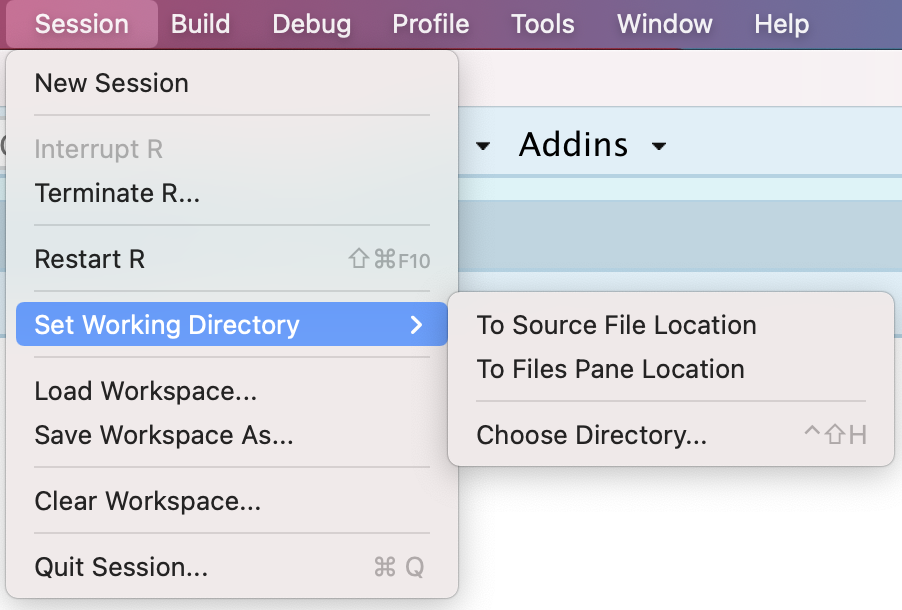
\includegraphics[width=0.9\linewidth]{pics/5_setwd} 

}

\caption{Set Working Directory}\label{fig:setwd1}
\end{figure}

There are three options under this menu:

\begin{itemize}
\tightlist
\item
  \emph{To Source File Location}: this will set the working directory as the directory of the current R script.
\item
  \emph{To Files Pane Location}: this will set the working directory as the directory of the Files Pane on the bottom right of RStudio.
\item
  \emph{Choose Directory\ldots{}}: this will open up a window from which you can choose any desired directory.
\end{itemize}

Keep in mind that if you choose to work under a RStudio project, you might notice an additional choice under the \emph{Set Working Directory} tab:

\begin{itemize}
\tightlist
\item
  \emph{To Project Directory}: this will set the working directory as the directory of your current RStudio project.
\end{itemize}

After selecting one of the three options, we can see a line of code containing the function \texttt{setwd()} executed in the console. Indeed, this menu operation is equivalent to using the \texttt{setwd()} function with the argument being the full path or relative path of the desired directory.

Another related function is \texttt{getwd()}, which tells us the absolute path representing the current working directory. When you see an error message saying that a file is not found, it is a good idea to check the current working directory and check whether it is correct.

\begin{Shaded}
\begin{Highlighting}[]
\FunctionTok{getwd}\NormalTok{()}
\end{Highlighting}
\end{Shaded}

For illustration purposes, we will create a folder called ``data'' using the function \texttt{dir.create()} under the current working directory and export/import to/from files in this folder.

\begin{Shaded}
\begin{Highlighting}[]
\FunctionTok{dir.create}\NormalTok{(}\StringTok{"data"}\NormalTok{)}
\end{Highlighting}
\end{Shaded}

\hypertarget{delimited-files}{%
\subsection{Delimited files}\label{delimited-files}}

In most applications, you will interact with the so-called \textbf{delimited} file. In a delimited file, each row represents a single observation, and it has values separated by the \textbf{delimiter}. In principle, \emph{any character (including letters, numbers, or symbols)} can be used as a delimiter, with the most commonly used ones being the follow.

\begin{tabular}{l|l|l}
\hline
Delimiter & Symbol & Common File Extension\\
\hline
comma & `,` & .csv\\
\hline
space & ` ` & .txt\\
\hline
tab & `\textbackslash{}t` & .tsv\\
\hline
\end{tabular}

\hypertarget{write-csv}{%
\subsection{Write an object into a .csv file}\label{write-csv}}

First, let's work with one popular kind of \emph{delimited} files called \emph{comma-separated value} file, usually with the file extension .csv. In a .csv file, the \emph{delimiter} is \emph{comma} (\texttt{,}).

Let's work with the \texttt{gm2007} dataset and export a part of it (first five rows and three columns) to a .csv file. To illustrate how the missing data affects data export, let's set the (3, 3) element to be \texttt{NA}. We have the country name, year, HDI for each of the 5 country we have here.

\begin{Shaded}
\begin{Highlighting}[]
\FunctionTok{library}\NormalTok{(r02pro)}
\NormalTok{gm\_small }\OtherTok{\textless{}{-}}\NormalTok{ gm2007[}\DecValTok{1}\SpecialCharTok{:}\DecValTok{5}\NormalTok{, }\DecValTok{1}\SpecialCharTok{:}\DecValTok{3}\NormalTok{]}
\NormalTok{gm\_small[}\DecValTok{3}\NormalTok{, }\DecValTok{3}\NormalTok{] }\OtherTok{\textless{}{-}} \ConstantTok{NA}
\NormalTok{gm\_small}
\CommentTok{\#\textgreater{} \# A tibble: 5 x 3}
\CommentTok{\#\textgreater{}   country               year continent}
\CommentTok{\#\textgreater{}   \textless{}chr\textgreater{}                \textless{}dbl\textgreater{} \textless{}chr\textgreater{}    }
\CommentTok{\#\textgreater{} 1 Afghanistan           2007 \textless{}NA\textgreater{}     }
\CommentTok{\#\textgreater{} 2 Angola                2007 Africa   }
\CommentTok{\#\textgreater{} 3 Albania               2007 \textless{}NA\textgreater{}     }
\CommentTok{\#\textgreater{} 4 Andorra               2007 \textless{}NA\textgreater{}     }
\CommentTok{\#\textgreater{} 5 United Arab Emirates  2007 Asia}
\end{Highlighting}
\end{Shaded}

Now, let's write the data frame \texttt{gm\_small} into a file called ``gm\_small.csv'' in the currently working directory. To write an object into a .csv file, you can use the \texttt{write\_csv()} function in the \textbf{readr} package. Since \textbf{readr} is a sub-package of \textbf{tidyverse}, you can load the package directly if the \textbf{tidyverse} package is installed.

\begin{Shaded}
\begin{Highlighting}[]
\FunctionTok{library}\NormalTok{(readr)}
\FunctionTok{write\_csv}\NormalTok{(gm\_small, }\StringTok{"data/gm\_small.csv"}\NormalTok{)}
\end{Highlighting}
\end{Shaded}

Note here, we are writing the tibble \texttt{gm\_small} into a file named ``gm\_small.csv'' in the folder ``data''. ``data/gm\_small.csv'' is an example of \textbf{relative file path}. You can also use the \textbf{absolute file path} on your computer, though it is not as collaboration friendly as the relative path, since your collaborator may have a different file structure from yours.

You can verify the .csv file has been indeed created and open the file with RStudio or any text editor to verify its contents.

\begin{figure}

{\centering 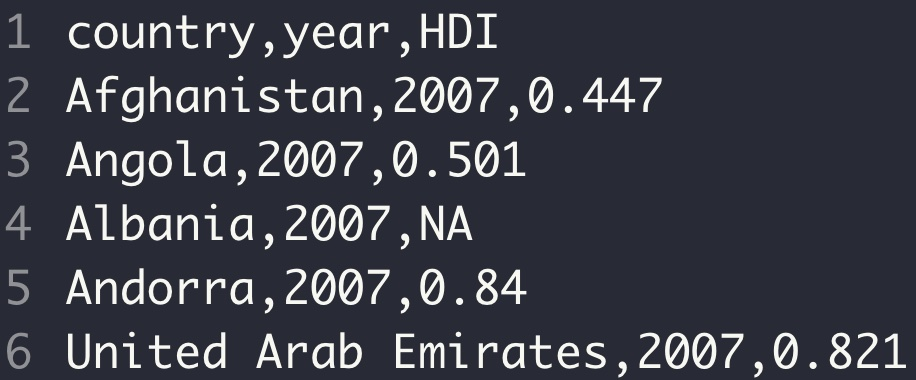
\includegraphics[width=0.9\linewidth]{pics/4.2_csv_content} 

}

\caption{File Contents}\label{fig:csv}
\end{figure}

We can see that all the information is wrote in the .csv file, with \emph{commas} separating the values on each observation. In particular, you may find out the first row of the file corresponds to the column names. If you don't want to include the column names, you can set the argument \texttt{col\_names\ =\ FALSE}.

\begin{Shaded}
\begin{Highlighting}[]
\FunctionTok{write\_csv}\NormalTok{(gm\_small, }\StringTok{"data/gm\_small\_no\_colname.csv"}\NormalTok{, }\AttributeTok{col\_names =} \ConstantTok{FALSE}\NormalTok{)}
\end{Highlighting}
\end{Shaded}

By default, \texttt{write\_csv()} writes the data into a file in which \texttt{NA} is used to represent all the missing values, just like in the tibble. If you want to use another string to represent the missing values in the file, you can set the argument \texttt{na} to be the string.

\begin{Shaded}
\begin{Highlighting}[]
\FunctionTok{write\_csv}\NormalTok{(gm\_small, }\StringTok{"data/gm\_small\_missing.csv"}\NormalTok{, }\AttributeTok{na =} \StringTok{"This value is missing!"}\NormalTok{)}
\end{Highlighting}
\end{Shaded}

\hypertarget{write-delim}{%
\subsection{Write an object into a general delimited file}\label{write-delim}}

As introduced at the beginning, there are different types of \emph{delimited files}, depending on the specific \emph{delimiter} of your choice. The function \texttt{write\_delim()} enables us to write an object into a delimited file with any chosen delimiter. The usage of \texttt{write\_delim()} is almost identical to \texttt{write\_csv()}, except that it has an additional argument \texttt{delim}, which specifies the delimiter to be used. Let's see the following example with \texttt{*} as the delimiter.

\begin{Shaded}
\begin{Highlighting}[]
\FunctionTok{write\_delim}\NormalTok{(gm\_small, }\StringTok{"data/gm\_small\_star.csv"}\NormalTok{, }\AttributeTok{delim =} \StringTok{"*"}\NormalTok{)}
\end{Highlighting}
\end{Shaded}

\hypertarget{exercises-27}{%
\subsection{Exercises}\label{exercises-27}}

Use R to create the following data frame and assign it to the name \texttt{my\_data}.

\begin{verbatim}
#>   word number letter
#> 1  one      1      a
#> 2  two     NA      b
#> 3 <NA>      3      c
#> 4 four      4      d
#> 5 five      5      e
\end{verbatim}

\begin{enumerate}
\def\labelenumi{\arabic{enumi}.}
\item
  Write R code to set working directory to the location of your .R or .Rmd file, and export \texttt{my\_data} into a .csv file named ``my\_data\_no\_name.csv'' without column names.
\item
  Write R code to export \texttt{my\_data} into a delimited file called ``my\_data\_na.csv'' with \texttt{\#} as the delimiter and use \texttt{999} as the indicator for missing values.
\end{enumerate}

\hypertarget{import-data}{%
\section{Importing Data from Delimited Files}\label{import-data}}

Knowing how to export data into delimited files, let us now see how to \textbf{import} data from delimited files.

\hypertarget{import-.csv-files-using-read_csv}{%
\subsection{\texorpdfstring{Import .csv Files using \texttt{read\_csv()}}{Import .csv Files using read\_csv()}}\label{import-.csv-files-using-read_csv}}

To import .csv files, we can use the function \texttt{read\_csv()} in the \textbf{readr} package, which is a sub-package of \textbf{tidyverse}. If you have already installed \textbf{tidyverse}, you can directly load the \textbf{readr} package.

After loading the \textbf{readr} package, you can try to import the data from ``gm\_small.csv'' which we created in Section \ref{write-csv}. Please make sure the .csv file is located in the folder ``data'' relative to the current working directory. Otherwise, you need to change the working directory accordingly using the methods introduced in Section \ref{setwd}.

\begin{Shaded}
\begin{Highlighting}[]
\FunctionTok{library}\NormalTok{(readr)}
\NormalTok{gm\_small }\OtherTok{\textless{}{-}} \FunctionTok{read\_csv}\NormalTok{(}\StringTok{"data/gm\_small.csv"}\NormalTok{)}
\CommentTok{\#\textgreater{} }
\CommentTok{\#\textgreater{} {-}{-} Column specification {-}{-}{-}{-}{-}{-}{-}{-}{-}{-}{-}{-}{-}{-}{-}{-}{-}{-}{-}{-}{-}{-}{-}{-}{-}{-}{-}{-}{-}{-}{-}{-}{-}{-}{-}{-}{-}{-}{-}{-}{-}{-}{-}{-}{-}{-}{-}{-}{-}{-}{-}{-}{-}{-}{-}{-}}
\CommentTok{\#\textgreater{} cols(}
\CommentTok{\#\textgreater{}   country = col\_character(),}
\CommentTok{\#\textgreater{}   year = col\_double(),}
\CommentTok{\#\textgreater{}   HDI = col\_double()}
\CommentTok{\#\textgreater{} )}
\end{Highlighting}
\end{Shaded}

We can see that there is a message showing the \textbf{Column specification} during the import process. In particular, we see \texttt{country} is of type \emph{character}, and both \texttt{year} and \texttt{HDI} are of type \emph{double}. We can also check the value of \texttt{gm\_small} and its structure.

\begin{Shaded}
\begin{Highlighting}[]
\NormalTok{gm\_small}
\CommentTok{\#\textgreater{} \# A tibble: 5 x 3}
\CommentTok{\#\textgreater{}   country               year    HDI}
\CommentTok{\#\textgreater{}   \textless{}chr\textgreater{}                \textless{}dbl\textgreater{}  \textless{}dbl\textgreater{}}
\CommentTok{\#\textgreater{} 1 Afghanistan           2007  0.447}
\CommentTok{\#\textgreater{} 2 Angola                2007  0.501}
\CommentTok{\#\textgreater{} 3 Albania               2007 NA    }
\CommentTok{\#\textgreater{} 4 Andorra               2007  0.84 }
\CommentTok{\#\textgreater{} 5 United Arab Emirates  2007  0.821}
\FunctionTok{str}\NormalTok{(gm\_small)}
\CommentTok{\#\textgreater{} spec\_tbl\_df [5 x 3] (S3: spec\_tbl\_df/tbl\_df/tbl/data.frame)}
\CommentTok{\#\textgreater{}  $ country: chr [1:5] "Afghanistan" "Angola" "Albania" "Andorra" ...}
\CommentTok{\#\textgreater{}  $ year   : num [1:5] 2007 2007 2007 2007 2007}
\CommentTok{\#\textgreater{}  $ HDI    : num [1:5] 0.447 0.501 NA 0.84 0.821}
\CommentTok{\#\textgreater{}  {-} attr(*, "spec")=}
\CommentTok{\#\textgreater{}   .. cols(}
\CommentTok{\#\textgreater{}   ..   country = col\_character(),}
\CommentTok{\#\textgreater{}   ..   year = col\_double(),}
\CommentTok{\#\textgreater{}   ..   HDI = col\_double()}
\CommentTok{\#\textgreater{}   .. )}
\end{Highlighting}
\end{Shaded}

We can see that the tibble \texttt{gm\_small} is generated along with the correct column types. In order to introduce the various options associated with \texttt{read\_csv()} function, let's move on to the topic of \textbf{inline} .csv files next.

\hypertarget{read-inline-.csv-files}{%
\subsection{Read Inline .csv Files}\label{read-inline-.csv-files}}

The \texttt{read\_csv()} function not only can read files into R, it also accept \textbf{inline input} as its argument. While the inline input may not be commonly used in practice, it is particularly useful for learning how to use the function, and be able to handle various importing cases when dealing with real life datasets. Let's see an example.

\begin{Shaded}
\begin{Highlighting}[]
\FunctionTok{read\_csv}\NormalTok{(}\StringTok{"x,y,z}
\StringTok{          1,3,5}
\StringTok{          2,4,6"}\NormalTok{)}
\CommentTok{\#\textgreater{} \# A tibble: 2 x 3}
\CommentTok{\#\textgreater{}       x     y     z}
\CommentTok{\#\textgreater{}   \textless{}dbl\textgreater{} \textless{}dbl\textgreater{} \textless{}dbl\textgreater{}}
\CommentTok{\#\textgreater{} 1     1     3     5}
\CommentTok{\#\textgreater{} 2     2     4     6}
\end{Highlighting}
\end{Shaded}

This inline input example is equivalent to reading a .csv file with contents identical to those in quotes. You can see that a tibble with size of 2 by 3 is generated with the column names being \texttt{x}, \texttt{y} and \texttt{z}. From the argument, we can see that by default, the \textbf{first row} of the input data will be interpreted as the column names.

\textbf{\emph{a. No column names}}

If the first row of the input data doesn't correspond to the variable names, you need to set \texttt{col\_names\ =\ FALSE} as an additional argument in \texttt{read\_csv()}.

\begin{Shaded}
\begin{Highlighting}[]
\FunctionTok{read\_csv}\NormalTok{(}\StringTok{"x,y,z}
\StringTok{          1,3,5}
\StringTok{          2,4,6"}\NormalTok{, }\AttributeTok{col\_names =} \ConstantTok{FALSE}\NormalTok{)}
\CommentTok{\#\textgreater{} \# A tibble: 3 x 3}
\CommentTok{\#\textgreater{}   X1    X2    X3   }
\CommentTok{\#\textgreater{}   \textless{}chr\textgreater{} \textless{}chr\textgreater{} \textless{}chr\textgreater{}}
\CommentTok{\#\textgreater{} 1 x     y     z    }
\CommentTok{\#\textgreater{} 2 1     3     5    }
\CommentTok{\#\textgreater{} 3 2     4     6}
\end{Highlighting}
\end{Shaded}

Now, a tibble of 3 rows and 3 columns was generated, with the column names being \texttt{X1}, \texttt{X2}, and \texttt{X3}. Note that these are the default naming conventions in the function when you don't supply the column names in the file. Another thing worth mentioning is that all three variables are of \textbf{character} types, due to the fact that there are character values for all variables (\texttt{x}, \texttt{y}, and \texttt{z}).

\textbf{\emph{b. Skip the first few lines}}

Sometimes, the first few lines of your data file may be descriptions of the data, which you want to skip when importing into R. We can set the \texttt{skip} argument in the \texttt{read\_csv()} function to skip a certain number of lines.

\begin{Shaded}
\begin{Highlighting}[]
\FunctionTok{read\_csv}\NormalTok{(}\StringTok{"The first line }
\StringTok{          The second line}
\StringTok{          The third line}
\StringTok{          x,y,z}
\StringTok{          1,3,5"}\NormalTok{, }\AttributeTok{skip =} \DecValTok{3}\NormalTok{)}
\CommentTok{\#\textgreater{} \# A tibble: 1 x 3}
\CommentTok{\#\textgreater{}       x     y     z}
\CommentTok{\#\textgreater{}   \textless{}dbl\textgreater{} \textless{}dbl\textgreater{} \textless{}dbl\textgreater{}}
\CommentTok{\#\textgreater{} 1     1     3     5}
\end{Highlighting}
\end{Shaded}

It is clear from the result that the first 3 lines of the input data are skipped.

\textbf{\emph{c.~Skip the comments}}

Another useful argument in cases when we have comments in the data file is the \texttt{comment} argument, which tells R to skip all text after the string specified in the \texttt{comment} argument.

\begin{Shaded}
\begin{Highlighting}[]
\FunctionTok{read\_csv}\NormalTok{(}\StringTok{"x,y,z \#variable names}
\StringTok{         1,3,5 \#the first observation}
\StringTok{         2,4,6 \#the second observation"}\NormalTok{, }\AttributeTok{comment =} \StringTok{"\#"}\NormalTok{)}
\CommentTok{\#\textgreater{} \# A tibble: 2 x 3}
\CommentTok{\#\textgreater{}       x     y     z}
\CommentTok{\#\textgreater{}   \textless{}dbl\textgreater{} \textless{}dbl\textgreater{} \textless{}dbl\textgreater{}}
\CommentTok{\#\textgreater{} 1     1     3     5}
\CommentTok{\#\textgreater{} 2     2     4     6}
\end{Highlighting}
\end{Shaded}

\hypertarget{handling-missing-values}{%
\subsection{Handling Missing Values}\label{handling-missing-values}}

In many real data sets, we may have missing values. You may recall that R uses \texttt{NA} to represent the missing values. If the data set was prepared by an R user, it probably already uses \texttt{NA} to represent all missing values. In this case, life is easy since \texttt{read\_csv()} will automatically interpret all \texttt{NA}s as missing values.

\begin{Shaded}
\begin{Highlighting}[]
\FunctionTok{read\_csv}\NormalTok{(}\StringTok{"x,y,z}
\StringTok{          999,3,5}
\StringTok{         NA,{-}999,6"}\NormalTok{)}
\CommentTok{\#\textgreater{} \# A tibble: 2 x 3}
\CommentTok{\#\textgreater{}       x     y     z}
\CommentTok{\#\textgreater{}   \textless{}dbl\textgreater{} \textless{}dbl\textgreater{} \textless{}dbl\textgreater{}}
\CommentTok{\#\textgreater{} 1   999     3     5}
\CommentTok{\#\textgreater{} 2    NA  {-}999     6}
\end{Highlighting}
\end{Shaded}

In a typical application, however, the person who prepared the data may use other strings to represent missing values. For example, if 999 and -999 are used as the indicators for missing values, you can set the argument \texttt{na} to be the vector containing those values, along with the default \texttt{NA} as a character.

\begin{Shaded}
\begin{Highlighting}[]
\FunctionTok{read\_csv}\NormalTok{(}\StringTok{"x,y,z}
\StringTok{          999,3, yes}
\StringTok{         NA,{-}999, no}
\StringTok{         12, 12, NA"}\NormalTok{, }\AttributeTok{na =} \FunctionTok{c}\NormalTok{(}\StringTok{"999"}\NormalTok{,}\StringTok{"{-}999"}\NormalTok{, }\StringTok{"NA"}\NormalTok{))}
\CommentTok{\#\textgreater{} \# A tibble: 3 x 3}
\CommentTok{\#\textgreater{}       x     y z    }
\CommentTok{\#\textgreater{}   \textless{}dbl\textgreater{} \textless{}dbl\textgreater{} \textless{}chr\textgreater{}}
\CommentTok{\#\textgreater{} 1    NA     3 yes  }
\CommentTok{\#\textgreater{} 2    NA    NA no   }
\CommentTok{\#\textgreater{} 3    12    12 \textless{}NA\textgreater{}}
\end{Highlighting}
\end{Shaded}

You can see from the output tibble that all the missing values are now denoted as \texttt{NA}.

::: \{.infobox .caution data-latex=``\{caution\}''\}
Note that the quotation marks around 999 and -999 are necessary since the \texttt{na} argument is expecting a character vector.

\begin{Shaded}
\begin{Highlighting}[]
\FunctionTok{read\_csv}\NormalTok{(}\StringTok{"x,y,z}
\StringTok{          999,3,5}
\StringTok{         999,{-}999,6"}\NormalTok{, }\AttributeTok{na =} \FunctionTok{c}\NormalTok{(}\DecValTok{999}\NormalTok{,}\SpecialCharTok{{-}}\DecValTok{999}\NormalTok{, }\ConstantTok{NA}\NormalTok{))}
\CommentTok{\#\textgreater{} Error in guess\_header\_(datasource, tokenizer, locale): Invalid input type, expected \textquotesingle{}character\textquotesingle{} actual \textquotesingle{}double\textquotesingle{}}
\end{Highlighting}
\end{Shaded}

You can see an error message, stating that it is expecting character values, but got double values.

In addition, the quotes around \texttt{NA} is also necessary.

\begin{Shaded}
\begin{Highlighting}[]
\FunctionTok{read\_csv}\NormalTok{(}\StringTok{"x,y,z}
\StringTok{          999,3, yes}
\StringTok{         NA,{-}999, no}
\StringTok{         12, 12, NA"}\NormalTok{, }\AttributeTok{na =} \FunctionTok{c}\NormalTok{(}\StringTok{"999"}\NormalTok{,}\StringTok{"{-}999"}\NormalTok{, }\ConstantTok{NA}\NormalTok{))}
\CommentTok{\#\textgreater{} \# A tibble: 3 x 3}
\CommentTok{\#\textgreater{}       x     y z    }
\CommentTok{\#\textgreater{}   \textless{}dbl\textgreater{} \textless{}dbl\textgreater{} \textless{}chr\textgreater{}}
\CommentTok{\#\textgreater{} 1    NA     3 yes  }
\CommentTok{\#\textgreater{} 2    NA    NA no   }
\CommentTok{\#\textgreater{} 3    12    12 \textless{}NA\textgreater{}}
\end{Highlighting}
\end{Shaded}

Here, the first column is wrongly interpreted as a character vector.

\hypertarget{importing-data-from-a-delimited-file}{%
\subsection{Importing Data From a Delimited File}\label{importing-data-from-a-delimited-file}}

You now know how to import data from a .csv file using the \texttt{read\_csv()} function. More generally, \texttt{read\_delim()} allows us to import data from a delimited file with any chosen \emph{delimiter}. The usage of \texttt{read\_delim()} is almost identical to \texttt{read\_csv()}, except that it has an additional argument \texttt{delim}, which specifies the delimiter to be used. Let's see the following example with \texttt{*} as the delimiter. Note that we are using the ``my\_animals\_star.csv'' file generated in Section \ref{write-delim}.

\begin{Shaded}
\begin{Highlighting}[]
\NormalTok{my\_animals }\OtherTok{\textless{}{-}} \FunctionTok{read\_delim}\NormalTok{(}\StringTok{"data/gm\_small\_star.csv"}\NormalTok{, }\AttributeTok{delim =} \StringTok{"*"}\NormalTok{)}
\end{Highlighting}
\end{Shaded}

Let's try to use \texttt{read\_csv()} instead to check what will you get.

\begin{Shaded}
\begin{Highlighting}[]
\FunctionTok{read\_csv}\NormalTok{(}\StringTok{"data/gm\_small\_star.csv"}\NormalTok{)}
\CommentTok{\#\textgreater{} }
\CommentTok{\#\textgreater{} {-}{-} Column specification {-}{-}{-}{-}{-}{-}{-}{-}{-}{-}{-}{-}{-}{-}{-}{-}{-}{-}{-}{-}{-}{-}{-}{-}{-}{-}{-}{-}{-}{-}{-}{-}{-}{-}{-}{-}{-}{-}{-}{-}{-}{-}{-}{-}{-}{-}{-}{-}{-}{-}{-}{-}{-}{-}{-}{-}}
\CommentTok{\#\textgreater{} cols(}
\CommentTok{\#\textgreater{}   \textasciigrave{}country*year*HDI\textasciigrave{} = col\_character()}
\CommentTok{\#\textgreater{} )}
\CommentTok{\#\textgreater{} \# A tibble: 5 x 1}
\CommentTok{\#\textgreater{}   \textasciigrave{}country*year*HDI\textasciigrave{}             }
\CommentTok{\#\textgreater{}   \textless{}chr\textgreater{}                          }
\CommentTok{\#\textgreater{} 1 Afghanistan*2007*0.447         }
\CommentTok{\#\textgreater{} 2 Angola*2007*0.501              }
\CommentTok{\#\textgreater{} 3 Albania*2007*NA                }
\CommentTok{\#\textgreater{} 4 Andorra*2007*0.84              }
\CommentTok{\#\textgreater{} 5 United Arab Emirates*2007*0.821}
\end{Highlighting}
\end{Shaded}

You will see that the imported data has only one variable named \texttt{country*year*HDI} since the function will interpret the whole thing as a single variable.

\hypertarget{import-menu}{%
\subsection{Import Data Using the Menu}\label{import-menu}}

Besides writing codes involving \texttt{read\_csv()} or \texttt{read\_delim()} to import data, you can also take advantage of the interactive menu RStudio provides.

To do this, you can click on the \textbf{Import Dataset} button in the \textbf{Environment} panel on the top right of RStudio shown in the following figure.

\begin{figure}

{\centering 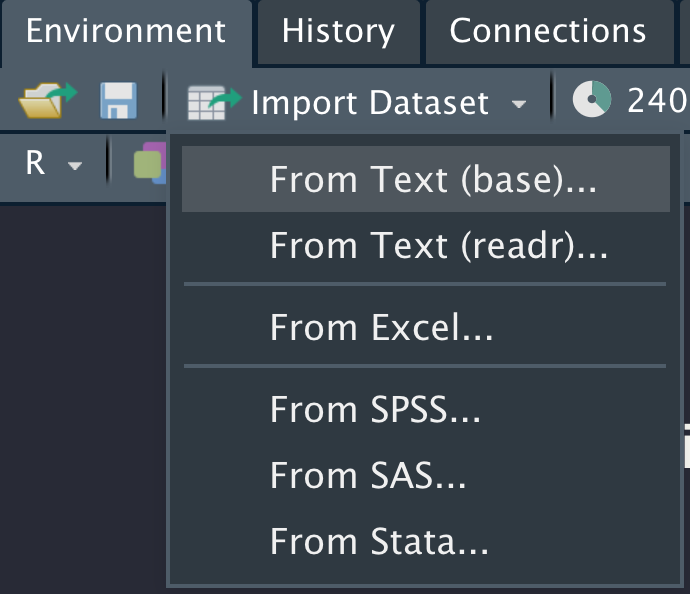
\includegraphics[width=0.9\linewidth]{pics/5-import} 

}

\caption{Import Dataset Menu}\label{fig:unnamed-chunk-493}
\end{figure}

Here, you can see quite a few options which are summarized in the following table.

\begin{table}

\caption{\label{tab:importMenu}Import Data from Menu}
\centering
\begin{tabular}[t]{l|l}
\hline
Choice & Name\\
\hline
From Text (readr) & Delimited Files (.csv, .txt, and others)\\
\hline
From Excel & Excel Files (.xls and .xlsx)\\
\hline
From SPSS & SPSS Files (.sav)\\
\hline
From SAS & SAS Files (.sas7bdat and.sas7bcat)\\
\hline
From Stata & Stata Files (.dta)\\
\hline
\end{tabular}
\end{table}

We will focus on importing delimited files in this section. We will cover importing Excel files in Section \ref{import-excel}. Working with SPSS, SAS, and Stata files will be covered in Section \ref{import-other}.

For importing a .csv file, .txt file, or any other file with a delimiter, you can choose the \textbf{From Text (readr)} option. Then, you can click \textbf{Browse\ldots{}} and select the data file. We will select the ``gm\_small\_star.csv'' file in the ``data'' folder.

After a file is selected, you can see the \textbf{Data Preview} which is showing the first several rows of the data. Note that the first row shows the column names and their associate types in parentheses. For each column, you can click the drop-down menu after the type to change its type.

\begin{figure}

{\centering 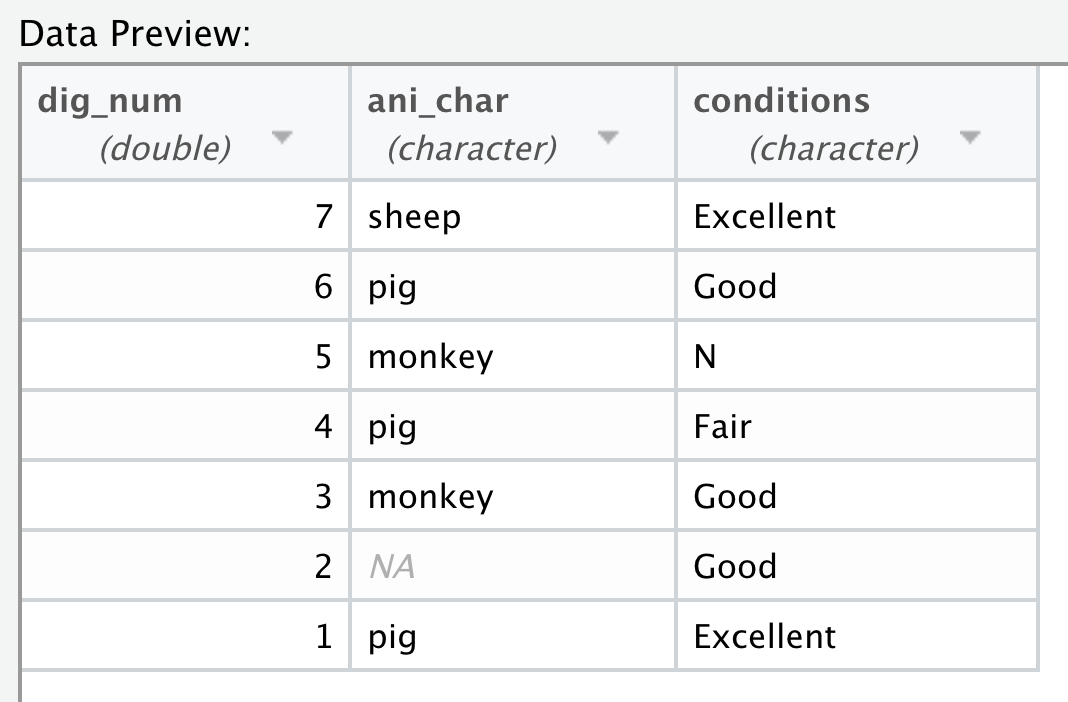
\includegraphics[width=0.9\linewidth]{pics/5-import-preview-star} 

}

\caption{Import Data Preview}\label{fig:unnamed-chunk-494}
\end{figure}

From this figure, you can see that the preview only shows one column named ``country*year*HDI''. Apparently, the separator ``*'' is not properly interpreted during the process.

To fix this problem, we can look at the \textbf{Import Options} in the left area.

\begin{figure}

{\centering 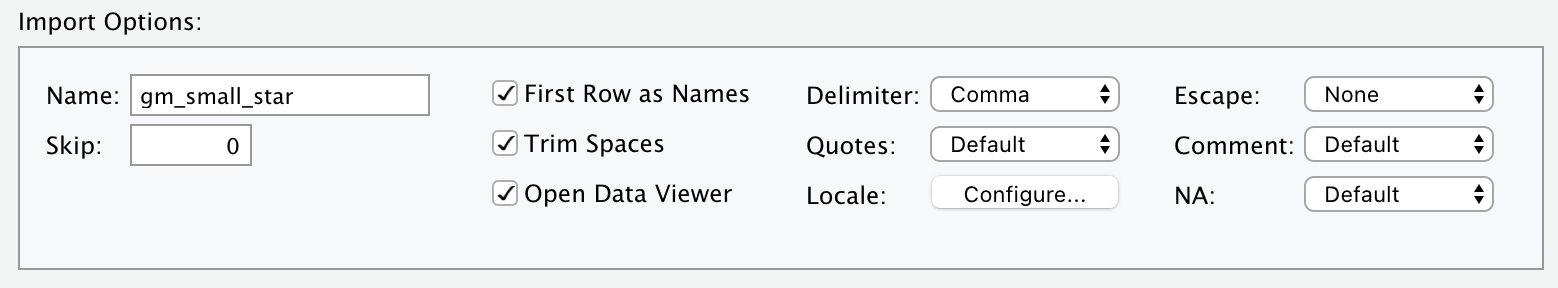
\includegraphics[width=0.9\linewidth]{pics/5-import-options} 

}

\caption{Import Options}\label{fig:unnamed-chunk-495}
\end{figure}

Let's summarize a few commonly used options, their corresponding arguments in the \texttt{read\_csv()} or \texttt{read\_delim()} function, and meanings.

\textbackslash begin\{table\}

\textbackslash caption\{\label{tab:importOptions}Menu Options and its Corresponding Arguments in \texttt{read\_delim()} and Meanings\}
\centering

\begin{tabular}[t]{l|l|l}
\hline
Option & Argument & Meaning\\
\hline
Name & - & The object name you would like to assign to.\\
\hline
Skip & `skip` & The number of rows to skip at the beginning of the file.\\
\hline
First Row as Names & `col\_names` & Whether you want to use the first row as column names. `TRUE` or `FALSE`.\\
\hline
Delimiter & `delim` & The delimiter of the data file.\\
\hline
Comment & `comment` & The character indicating the starting of comment. The contents after the comment character will be ignore in each line.\\
\hline
NA & `na` & The way NA is represented in the data file.\\
\hline
Code Preview & - & The R code to be executed for importing the data\\
\hline
\end{tabular}

\textbackslash end\{table\}

In our case, we will change the value of ``Delimiter'' to ``*'' (Note that you need to select ``Other..'', and enter ``*'' manually.)

\begin{figure}

{\centering 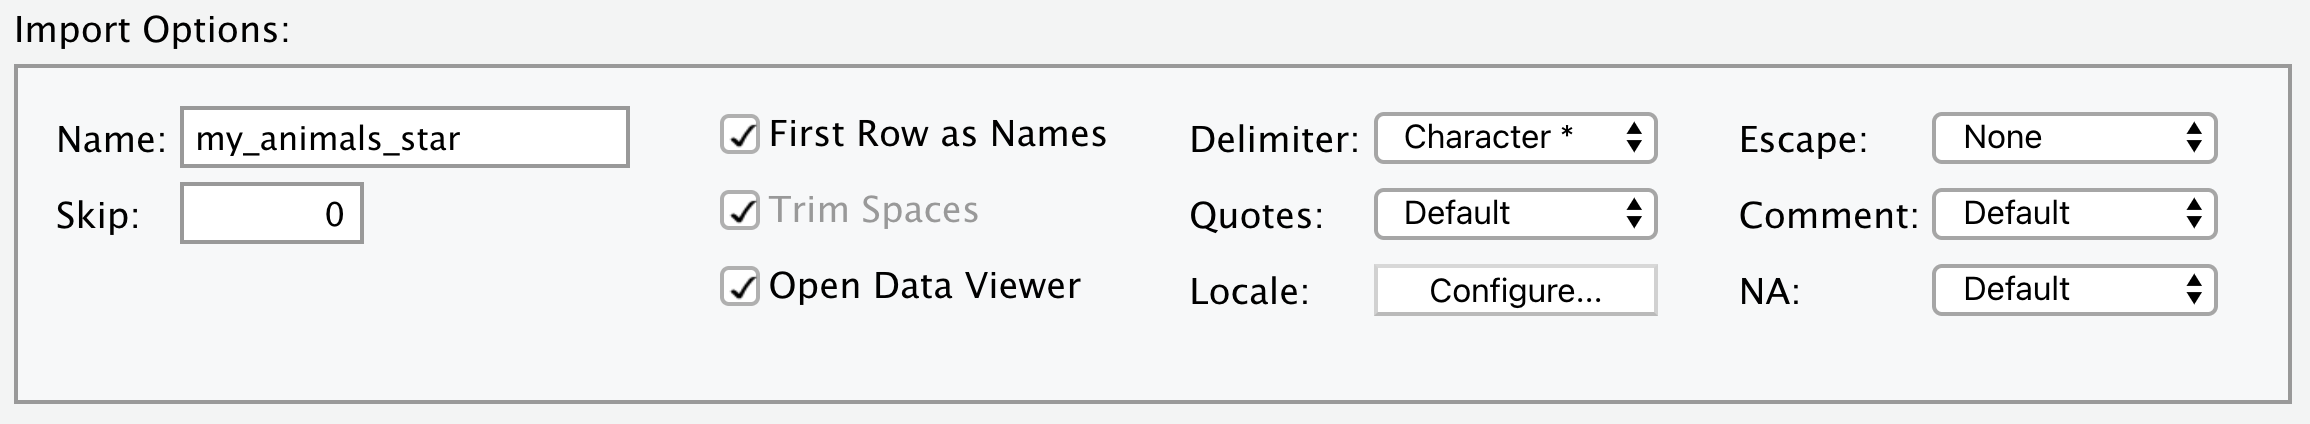
\includegraphics[width=0.9\linewidth]{pics/5-import-options-star} 

}

\caption{Import Options (Star)}\label{fig:unnamed-chunk-496}
\end{figure}

Note that when you change the delimiter, the \textbf{Data Preview} window also change correspondingly.

\begin{figure}

{\centering 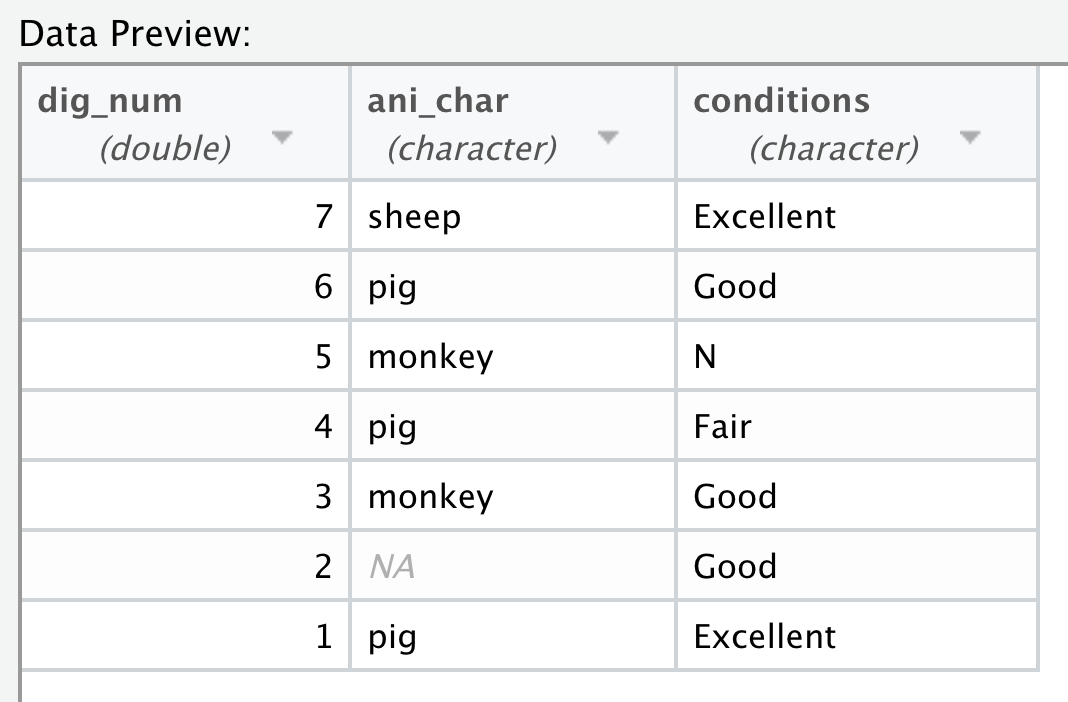
\includegraphics[width=0.9\linewidth]{pics/5-import-preview-star} 

}

\caption{Data Preview (Star)}\label{fig:unnamed-chunk-497}
\end{figure}

After changing the delimiter to \texttt{*}, we are seeing the expected data with three columns: \texttt{dig\_num}, \texttt{ani\_char}, and \texttt{conditions}.

The code in the \emph{Code Preview} window will change accordingly, which is a great way to learn on how they work. The new codes in the \emph{Code Preview} window is as below.

\begin{Shaded}
\begin{Highlighting}[]
\FunctionTok{library}\NormalTok{(readr)}
\NormalTok{gm\_small\_star }\OtherTok{\textless{}{-}} \FunctionTok{read\_delim}\NormalTok{(}\StringTok{"data/gm\_small\_star.csv"}\NormalTok{, }
                            \AttributeTok{delim =} \StringTok{"*"}\NormalTok{, }
                            \AttributeTok{escape\_double =} \ConstantTok{FALSE}\NormalTok{, }
                            \AttributeTok{trim\_ws =} \ConstantTok{TRUE}\NormalTok{)}
\FunctionTok{View}\NormalTok{(gm\_small\_star)}
\end{Highlighting}
\end{Shaded}

\hypertarget{exercises-28}{%
\subsection{Exercises}\label{exercises-28}}

\begin{enumerate}
\def\labelenumi{\arabic{enumi}.}
\item
  For the ``my\_data\_na.csv'' file you created in Exercise 2 in Section \ref{export-data}, write R code to read the file into an object with name \texttt{my\_data}.
\item
  First, look at the code below.
\end{enumerate}

\begin{Shaded}
\begin{Highlighting}[]
\NormalTok{d1 }\OtherTok{\textless{}{-}} \FunctionTok{read\_csv}\NormalTok{(}\StringTok{"x,y,z}
\StringTok{          1,3,5}
\StringTok{          2,4,6"}\NormalTok{, }\AttributeTok{col\_names =} \ConstantTok{FALSE}\NormalTok{)}
\end{Highlighting}
\end{Shaded}

Which of the following are the column names of the \texttt{d1}?

\begin{itemize}
\tightlist
\item
  \texttt{X1}, \texttt{X2}, and \texttt{X3}
\item
  \texttt{x}, \texttt{y}, and \texttt{z}
\end{itemize}

\begin{enumerate}
\def\labelenumi{\arabic{enumi}.}
\setcounter{enumi}{2}
\tightlist
\item
  First, look at the code below.
\end{enumerate}

\begin{Shaded}
\begin{Highlighting}[]
\NormalTok{d1 }\OtherTok{\textless{}{-}} \FunctionTok{read\_csv}\NormalTok{(}\StringTok{"The first line }
\StringTok{          The second line}
\StringTok{          The third line}
\StringTok{          x,y,z}
\StringTok{          1,3,5"}\NormalTok{)}
\end{Highlighting}
\end{Shaded}

What will be the column name(s) of the \texttt{d1}?

\hypertarget{import-excel}{%
\section{Exporting to and Importing from Excel Files}\label{import-excel}}

Now, you know how to export to and import from \emph{delimited} files. In this section, you will learn how to export to and import from Excel files with extensions .xls and .xlxs.

\hypertarget{export-data-into-excel-files}{%
\subsection{Export data into Excel files}\label{export-data-into-excel-files}}

To export data into an Excel file, you can use the \textbf{writexl} package. Let's first install the package.

\begin{Shaded}
\begin{Highlighting}[]
\FunctionTok{install.packages}\NormalTok{(}\StringTok{"writexl"}\NormalTok{)}
\end{Highlighting}
\end{Shaded}

Now, we can load the \textbf{writexl} package and use the \texttt{write\_xlsx()} function to write data into an Excel file with extension .xlsx. Let's first load the data from ``gm\_small.csv'' and write it to ``gm\_small.xlsx''.

\begin{Shaded}
\begin{Highlighting}[]
\FunctionTok{library}\NormalTok{(writexl)}
\FunctionTok{library}\NormalTok{(readr)}
\NormalTok{gm\_small }\OtherTok{\textless{}{-}} \FunctionTok{read\_csv}\NormalTok{(}\StringTok{"data/gm\_small.csv"}\NormalTok{)}
\FunctionTok{write\_xlsx}\NormalTok{(gm\_small, }\StringTok{"data/gm\_small.xlsx"}\NormalTok{)}
\end{Highlighting}
\end{Shaded}

By default, the column names of the data frame/tibble will be written to the first row of the Excel file. To skip the column names, you can set \texttt{col\_names\ =\ FALSE} in the \texttt{write\_xlsx()} function.

In addition to writing a single data frame to an Excel file, \texttt{write\_xlsx()} can also write \textbf{multiple data frames} into a single Excel file, with each Excel sheet containing one data frame. To do that, you need to supply a list of data frames as the first argument in \texttt{write\_xlsx()}. Let's take a look at the following example which write both \texttt{gm\_small} and \texttt{sahp} (a tibble in the \textbf{r02pro} package introduced in Section \ref{sahp}) into an Excel file named ``two\_data.xlsx''.

\begin{Shaded}
\begin{Highlighting}[]
\FunctionTok{library}\NormalTok{(r02pro)}
\NormalTok{two\_data }\OtherTok{\textless{}{-}} \FunctionTok{list}\NormalTok{(}\AttributeTok{gapminder =}\NormalTok{ gm\_small, }\AttributeTok{sahp =}\NormalTok{ sahp)}
\FunctionTok{write\_xlsx}\NormalTok{(two\_data, }\StringTok{"data/two\_data.xlsx"}\NormalTok{)}
\end{Highlighting}
\end{Shaded}

You can open this file with Excel and verify its contents.

\hypertarget{import-excel-files-.xls-and-.xlsx-using-read_excel}{%
\subsection{\texorpdfstring{Import Excel Files (.xls and .xlsx ) using \texttt{read\_excel()}}{Import Excel Files (.xls and .xlsx ) using read\_excel()}}\label{import-excel-files-.xls-and-.xlsx-using-read_excel}}

After learning how to export data into an Excel file, let's see how to read an existing Excel file into R. We can use the \texttt{read\_excel()} function in the \texttt{readxl} package to import Excel files. Here, \texttt{readxl} is another subpackage in the \textbf{tidyverse} package. Thus we can directly load the package if the \textbf{tidyverse} package is already installed.

Let's import the Excel file ``two\_data.xlsx'' we just created into R.

\begin{Shaded}
\begin{Highlighting}[]
\FunctionTok{library}\NormalTok{(readxl)}
\NormalTok{my\_df }\OtherTok{\textless{}{-}} \FunctionTok{read\_excel}\NormalTok{(}\StringTok{"data/two\_data.xlsx"}\NormalTok{)}
\FunctionTok{head}\NormalTok{(my\_df)}
\CommentTok{\#\textgreater{} \# A tibble: 5 x 3}
\CommentTok{\#\textgreater{}   country               year    HDI}
\CommentTok{\#\textgreater{}   \textless{}chr\textgreater{}                \textless{}dbl\textgreater{}  \textless{}dbl\textgreater{}}
\CommentTok{\#\textgreater{} 1 Afghanistan           2007  0.447}
\CommentTok{\#\textgreater{} 2 Angola                2007  0.501}
\CommentTok{\#\textgreater{} 3 Albania               2007 NA    }
\CommentTok{\#\textgreater{} 4 Andorra               2007  0.84 }
\CommentTok{\#\textgreater{} 5 United Arab Emirates  2007  0.821}
\end{Highlighting}
\end{Shaded}

We can see from the result that although the file contains two sheets, the function will import the first sheet by default. To import the second sheet, you can set the \texttt{sheet} argument to the sheet name (\texttt{sahp}) or the position of the sheet (2).

\begin{Shaded}
\begin{Highlighting}[]
\NormalTok{sahp\_1 }\OtherTok{\textless{}{-}} \FunctionTok{read\_excel}\NormalTok{(}\StringTok{"two\_data.xlsx"}\NormalTok{, }\AttributeTok{sheet =} \StringTok{"sahp"}\NormalTok{)}
\CommentTok{\#sahp\_1 \textless{}{-} read\_excel("two\_data.xlsx", sheet = 2)     \#same result as the previous line}
\FunctionTok{head}\NormalTok{(sahp\_1)}
\CommentTok{\#\textgreater{} \# A tibble: 6 x 13}
\CommentTok{\#\textgreater{}   dt\_sold             bedroom bathroom gar\_car oa\_qual liv\_area lot\_area}
\CommentTok{\#\textgreater{}   \textless{}dttm\textgreater{}                \textless{}dbl\textgreater{}    \textless{}dbl\textgreater{}   \textless{}dbl\textgreater{}   \textless{}dbl\textgreater{}    \textless{}dbl\textgreater{}    \textless{}dbl\textgreater{}}
\CommentTok{\#\textgreater{} 1 2010{-}03{-}25 00:00:00       3      2.5       2       6     1479    13517}
\CommentTok{\#\textgreater{} 2 2009{-}04{-}10 00:00:00       4      3.5       2       7     2122    11492}
\CommentTok{\#\textgreater{} 3 2010{-}01{-}15 00:00:00       3      2         1       5     1057     7922}
\CommentTok{\#\textgreater{} 4 2010{-}04{-}19 00:00:00       3      2.5       2       5     1444     9802}
\CommentTok{\#\textgreater{} 5 2010{-}03{-}22 00:00:00       3      2         2       6     1445    14235}
\CommentTok{\#\textgreater{} 6 2010{-}06{-}06 00:00:00       2      2.5       2       6     1888    16492}
\CommentTok{\#\textgreater{} \# ... with 6 more variables: house\_style \textless{}chr\textgreater{}, kit\_qual \textless{}chr\textgreater{},}
\CommentTok{\#\textgreater{} \#   heat\_qual \textless{}chr\textgreater{}, central\_air \textless{}chr\textgreater{}, sale\_price \textless{}dbl\textgreater{}, good\_qual \textless{}lgl\textgreater{}}
\end{Highlighting}
\end{Shaded}

If we only want to import a portion of the data, say the first 5 rows and the first 4 columns, then we can set the argument \texttt{range\ =\ "A1:D5"}, just like the range in an excel file. Note that the index starts with the first row, which may correspond to the column names.

\begin{Shaded}
\begin{Highlighting}[]
\NormalTok{sahp\_2 }\OtherTok{\textless{}{-}} \FunctionTok{read\_excel}\NormalTok{(}\StringTok{"two\_data.xlsx"}\NormalTok{, }\AttributeTok{sheet =} \StringTok{"sahp"}\NormalTok{, }\AttributeTok{range =} \StringTok{"A1:D5"}\NormalTok{)}
\NormalTok{sahp\_2}
\CommentTok{\#\textgreater{} \# A tibble: 4 x 4}
\CommentTok{\#\textgreater{}   dt\_sold             bedroom bathroom gar\_car}
\CommentTok{\#\textgreater{}   \textless{}dttm\textgreater{}                \textless{}dbl\textgreater{}    \textless{}dbl\textgreater{}   \textless{}dbl\textgreater{}}
\CommentTok{\#\textgreater{} 1 2010{-}03{-}25 00:00:00       3      2.5       2}
\CommentTok{\#\textgreater{} 2 2009{-}04{-}10 00:00:00       4      3.5       2}
\CommentTok{\#\textgreater{} 3 2010{-}01{-}15 00:00:00       3      2         1}
\CommentTok{\#\textgreater{} 4 2010{-}04{-}19 00:00:00       3      2.5       2}
\end{Highlighting}
\end{Shaded}

Note that \texttt{read\_excel()} can read both .xls and xlsx file types.

\hypertarget{import-excel-file-using-the-menu}{%
\subsection{Import Excel file using the menu}\label{import-excel-file-using-the-menu}}

Besides using \texttt{read\_excel()} to import Excel files, you can again use the interactive menu we introduced in Section \ref{import-data}.

As introduced in Table \ref{tab:importMenu}, to import Excel files, you can select \emph{From Excel} after choosing the \textbf{Import Dataset} option. As before, you can click \textbf{Browse\ldots{}} and select the data file. Let's select the ``two\_data.xlsx'' file we just created.

Similar to importing the delimited files, we can see the first several rows in the \textbf{Data Preview} window. The first row shows the column names and their associate types in parentheses. For each column, you can click the dropdown menu after the type to change its type. Now, let's discuss several options in the \textbf{Import Options} section and their corresponding arguments in the \texttt{read\_excel()} function.

\textbackslash begin\{table\}

\textbackslash caption\{\label{tab:importExcelOptions}Menu Options and its Corresponding Arguments in \texttt{read\_excel()} and Meanings\}
\centering

\begin{tabular}[t]{l|l|l}
\hline
Option & Argument & Meaning\\
\hline
Name & - & The object name you would like to assign to.\\
\hline
Sheet & `sheet` & The Sheet you want to import from.\\
\hline
Range & `range` & The data range you want to import.\\
\hline
Max Rows & `n\_max` & The maximum number of rows to import.\\
\hline
Skip & `skip` & The number of rows to skip at the beginning of the file.\\
\hline
NA & `na` & The way NA is represented in the data file.\\
\hline
First Row as Names & `col\_names` & Whether you want to use the first row as column names. `TRUE` or `FALSE`.\\
\hline
Code Preview & - & The R code to be executed for importing the data\\
\hline
\end{tabular}

\textbackslash end\{table\}

Note that similar as importing delimited files, when you change these options, the code in the \emph{Code Preview} window will change accordingly, which is a great way to learn on how they work.

\hypertarget{exercises-29}{%
\subsection{Exercises}\label{exercises-29}}

Use R to create the following data frame and assign it to the name \texttt{df1}.

\begin{verbatim}
#>   word1 number1
#> 1   one       1
#> 2   two      NA
#> 3  <NA>       3
\end{verbatim}

Then, use R to create the following data frame and assign it to the name \texttt{df2}.

\begin{verbatim}
#>   word2 number2
#> 1 three       3
#> 2  <NA>       4
#> 3  five       5
\end{verbatim}

Then create a list named \texttt{my\_list} with \texttt{df1} as the first element and \texttt{df2} as the second element.

\begin{enumerate}
\def\labelenumi{\arabic{enumi}.}
\item
  Write R code to set working directory to the desktop, then export \texttt{my\_list} into an excel file named \texttt{list.xlsx}. How many sheets are there in the excel file? What's in each sheet?
\item
  Write R code to import the first two rows and the first column of the second sheet from the excel file you just created. And verify the object value.
\end{enumerate}

\hypertarget{import-other}{%
\section{Exporting to and Importing from SPSS, SAS, and Stata Files}\label{import-other}}

Now, you know how to export and import data from delimited files and Excel files. In the section, you will learn how to export and import data from other statistical software including SPSS, SAS, and Stata. We will use the package \textbf{haven}, another member of the \textbf{tidyverse} family.

\hypertarget{export-and-import-spss-files}{%
\subsection{Export and Import SPSS Files}\label{export-and-import-spss-files}}

Let's first load the package \textbf{haven}, and prepare a data frame for exporting.

\begin{Shaded}
\begin{Highlighting}[]
\FunctionTok{library}\NormalTok{(tibble)}
\FunctionTok{library}\NormalTok{(haven)}
\NormalTok{dig\_num }\OtherTok{\textless{}{-}} \DecValTok{7}\SpecialCharTok{:}\DecValTok{1}
\NormalTok{ani\_char }\OtherTok{\textless{}{-}} \FunctionTok{c}\NormalTok{(}\StringTok{"sheep"}\NormalTok{, }\StringTok{"pig"}\NormalTok{, }\StringTok{"monkey"}\NormalTok{, }\StringTok{"pig"}\NormalTok{, }\StringTok{"monkey"}\NormalTok{, }\ConstantTok{NA}\NormalTok{, }\StringTok{"pig"}\NormalTok{)}
\NormalTok{conditions }\OtherTok{\textless{}{-}} \FunctionTok{c}\NormalTok{(}\StringTok{"Excellent"}\NormalTok{, }\StringTok{"Good"}\NormalTok{, }\ConstantTok{NA}\NormalTok{, }\StringTok{"Fair"}\NormalTok{, }\StringTok{"Good"}\NormalTok{, }\StringTok{"Good"}\NormalTok{, }\StringTok{"Excellent"}\NormalTok{)}
\NormalTok{my\_animals}\OtherTok{\textless{}{-}} \FunctionTok{tibble}\NormalTok{(dig\_num, ani\_char,conditions)}
\NormalTok{my\_animals}
\CommentTok{\#\textgreater{} \# A tibble: 7 x 3}
\CommentTok{\#\textgreater{}   dig\_num ani\_char conditions}
\CommentTok{\#\textgreater{}     \textless{}int\textgreater{} \textless{}chr\textgreater{}    \textless{}chr\textgreater{}     }
\CommentTok{\#\textgreater{} 1       7 sheep    Excellent }
\CommentTok{\#\textgreater{} 2       6 pig      Good      }
\CommentTok{\#\textgreater{} 3       5 monkey   \textless{}NA\textgreater{}      }
\CommentTok{\#\textgreater{} 4       4 pig      Fair      }
\CommentTok{\#\textgreater{} 5       3 monkey   Good      }
\CommentTok{\#\textgreater{} 6       2 \textless{}NA\textgreater{}     Good      }
\CommentTok{\#\textgreater{} 7       1 pig      Excellent}
\end{Highlighting}
\end{Shaded}

The data frame \texttt{my\_animals} will be used as in Section \ref{export-data}. You can use the function \texttt{write\_sav()} to export a data frame into a SPSS .sav file.

\begin{Shaded}
\begin{Highlighting}[]
\FunctionTok{write\_sav}\NormalTok{(my\_animals, }\StringTok{"data/my\_animals.sav"}\NormalTok{)}
\end{Highlighting}
\end{Shaded}

To read a SPSS file ending in .sav or .por, you can use the function \texttt{read\_spss()} which will automatically call \texttt{read\_sav()} for .sav files and \texttt{read\_por()} for .por files.

\begin{Shaded}
\begin{Highlighting}[]
\NormalTok{my\_animals\_spss }\OtherTok{\textless{}{-}} \FunctionTok{read\_spss}\NormalTok{(}\StringTok{"data/my\_animals.sav"}\NormalTok{)}
\FunctionTok{head}\NormalTok{(my\_animals\_spss)}
\CommentTok{\#\textgreater{} \# A tibble: 6 x 3}
\CommentTok{\#\textgreater{}   dig\_num ani\_char conditions }
\CommentTok{\#\textgreater{}     \textless{}dbl\textgreater{} \textless{}chr\textgreater{}    \textless{}chr\textgreater{}      }
\CommentTok{\#\textgreater{} 1       7 "sheep"  "Excellent"}
\CommentTok{\#\textgreater{} 2       6 "pig"    "Good"     }
\CommentTok{\#\textgreater{} 3       5 "monkey" ""         }
\CommentTok{\#\textgreater{} 4       4 "pig"    "Fair"     }
\CommentTok{\#\textgreater{} 5       3 "monkey" "Good"     }
\CommentTok{\#\textgreater{} 6       2 ""       "Good"}
\end{Highlighting}
\end{Shaded}

\hypertarget{export-and-import-sas-files}{%
\subsection{Export and Import SAS Files}\label{export-and-import-sas-files}}

You can use the function \texttt{write\_sas()} to export a data frame into a SAS .sas7bdat file.

\begin{Shaded}
\begin{Highlighting}[]
\FunctionTok{write\_sas}\NormalTok{(my\_animals, }\StringTok{"data/my\_animals.sas7bdat"}\NormalTok{)}
\end{Highlighting}
\end{Shaded}

To import a SAS file, you can use the function \texttt{read\_sas()}.

\begin{Shaded}
\begin{Highlighting}[]
\NormalTok{my\_animals\_sas }\OtherTok{\textless{}{-}} \FunctionTok{read\_sas}\NormalTok{(}\StringTok{"data/my\_animals.sas7bdat"}\NormalTok{)}
\FunctionTok{head}\NormalTok{(my\_animals\_sas)}
\CommentTok{\#\textgreater{} \# A tibble: 6 x 3}
\CommentTok{\#\textgreater{}   dig\_num ani\_char conditions }
\CommentTok{\#\textgreater{}     \textless{}dbl\textgreater{} \textless{}chr\textgreater{}    \textless{}chr\textgreater{}      }
\CommentTok{\#\textgreater{} 1       7 "sheep"  "Excellent"}
\CommentTok{\#\textgreater{} 2       6 "pig"    "Good"     }
\CommentTok{\#\textgreater{} 3       5 "monkey" ""         }
\CommentTok{\#\textgreater{} 4       4 "pig"    "Fair"     }
\CommentTok{\#\textgreater{} 5       3 "monkey" "Good"     }
\CommentTok{\#\textgreater{} 6       2 ""       "Good"}
\end{Highlighting}
\end{Shaded}

\hypertarget{export-and-import-stata-files}{%
\subsection{Export and Import Stata Files}\label{export-and-import-stata-files}}

Lastly, let's talk about Stata files. You can use the function \texttt{write\_dta()} to export a data frame into a Stata .dta file.

\begin{Shaded}
\begin{Highlighting}[]
\FunctionTok{write\_dta}\NormalTok{(my\_animals, }\StringTok{"data/my\_animals.dta"}\NormalTok{)}
\end{Highlighting}
\end{Shaded}

To read a Stata file ending in .dta, you can use the function \texttt{read\_dta()}.

\begin{Shaded}
\begin{Highlighting}[]
\NormalTok{my\_animals\_stata }\OtherTok{\textless{}{-}} \FunctionTok{read\_dta}\NormalTok{(}\StringTok{"data/my\_animals.dta"}\NormalTok{)}
\FunctionTok{head}\NormalTok{(my\_animals\_stata)}
\CommentTok{\#\textgreater{} \# A tibble: 6 x 3}
\CommentTok{\#\textgreater{}   dig\_num ani\_char conditions }
\CommentTok{\#\textgreater{}     \textless{}dbl\textgreater{} \textless{}chr\textgreater{}    \textless{}chr\textgreater{}      }
\CommentTok{\#\textgreater{} 1       7 "sheep"  "Excellent"}
\CommentTok{\#\textgreater{} 2       6 "pig"    "Good"     }
\CommentTok{\#\textgreater{} 3       5 "monkey" ""         }
\CommentTok{\#\textgreater{} 4       4 "pig"    "Fair"     }
\CommentTok{\#\textgreater{} 5       3 "monkey" "Good"     }
\CommentTok{\#\textgreater{} 6       2 ""       "Good"}
\end{Highlighting}
\end{Shaded}

\hypertarget{import-using-the-menu}{%
\subsection{Import using the menu}\label{import-using-the-menu}}

Similarly as Sections \ref{import-data} and \ref{import-excel}, you can also use the menu in Table \ref{tab:importMenu} to import SPSS, SAS, and Stata Files.

\hypertarget{exercise}{%
\subsection{Exercise}\label{exercise}}

\begin{enumerate}
\def\labelenumi{\arabic{enumi}.}
\tightlist
\item
  Export the first 8 observations in the \texttt{sahp} dataset (in \textbf{r02pro} package) to SPSS, SAS, and Stata file formats, respectively.
\item
  Import the files from Q1 to R and verify their contents.
\end{enumerate}

\hypertarget{save-object}{%
\section{Save and Restore Objects and Workspace}\label{save-object}}

Now, you know how to export and import data frames (or tibbles) to and from various types of files. In this section, you will learn how to save and restore one or more objects that can be \textbf{of any types}, and even the \textbf{whole workspace} that includes all the named objects.

To get started, let's first clear our workspace using \texttt{rm(list\ =\ ls())} and create a few objects with different types.

\begin{Shaded}
\begin{Highlighting}[]
\FunctionTok{rm}\NormalTok{(}\AttributeTok{list =} \FunctionTok{ls}\NormalTok{())}
\NormalTok{dig\_num }\OtherTok{\textless{}{-}} \DecValTok{7}\SpecialCharTok{:}\DecValTok{1}
\NormalTok{ani\_char }\OtherTok{\textless{}{-}} \FunctionTok{c}\NormalTok{(}\StringTok{"sheep"}\NormalTok{, }\StringTok{"pig"}\NormalTok{, }\StringTok{"monkey"}\NormalTok{, }\StringTok{"pig"}\NormalTok{, }\StringTok{"monkey"}\NormalTok{, }\ConstantTok{NA}\NormalTok{, }\StringTok{"pig"}\NormalTok{)}
\end{Highlighting}
\end{Shaded}

Recall that we can use \texttt{ls()} to get a vector of strings giving the names of the objects in the current environment.

\begin{Shaded}
\begin{Highlighting}[]
\FunctionTok{ls}\NormalTok{()}
\CommentTok{\#\textgreater{} [1] "ani\_char" "dig\_num"}
\end{Highlighting}
\end{Shaded}

\hypertarget{save-and-restore-objects-using-.rdata}{%
\subsection{Save and Restore Objects using .RData}\label{save-and-restore-objects-using-.rdata}}

In R, you can use the function \texttt{save()} to save one or more objects into an .RData file. Note that you want to make sure to change the working directory as needed. Let's see the following example where we save the object \texttt{dig\_num} into a file named ``dig\_num.RData''.

\begin{Shaded}
\begin{Highlighting}[]
\FunctionTok{save}\NormalTok{(dig\_num, }\AttributeTok{file =} \StringTok{"data/dig\_num.RData"}\NormalTok{)}
\end{Highlighting}
\end{Shaded}

Before introducing how to restore objects, let's first remove \texttt{dig\_num} from our workspace using the \texttt{rm()} function and check its value.

\begin{Shaded}
\begin{Highlighting}[]
\FunctionTok{rm}\NormalTok{(dig\_num)}
\NormalTok{dig\_num}
\CommentTok{\#\textgreater{} Error in eval(expr, envir, enclos): object \textquotesingle{}dig\_num\textquotesingle{} not found}
\end{Highlighting}
\end{Shaded}

You can see an error since \texttt{dig\_num} has been removed from the workspace. To restore it, you can use the function \texttt{load()} with the corresponding .RData file in double quotes as its argument.

\begin{Shaded}
\begin{Highlighting}[]
\FunctionTok{load}\NormalTok{(}\StringTok{"data/dig\_num.RData"}\NormalTok{)}
\NormalTok{dig\_num}
\CommentTok{\#\textgreater{} [1] 7 6 5 4 3 2 1}
\end{Highlighting}
\end{Shaded}

You can verify from the value of \texttt{dig\_num} that we have successfully restored the object \texttt{dig\_num} from the file ``dig\_num.RData''.

To save more than one objects into a single file, you just need to enter them as additional arguments in the \texttt{save()} function.

\begin{Shaded}
\begin{Highlighting}[]
\FunctionTok{save}\NormalTok{(dig\_num, ani\_char, }\AttributeTok{file =} \StringTok{"data/dig\_num\_and\_ani\_char.RData"}\NormalTok{)}
\end{Highlighting}
\end{Shaded}

To save everything in the workspace, you can use the function \texttt{save.image()} with the desired file name in double quotes as the argument.

\begin{Shaded}
\begin{Highlighting}[]
\FunctionTok{save.image}\NormalTok{(}\StringTok{"data/all.RData"}\NormalTok{)}
\end{Highlighting}
\end{Shaded}

To verify that ``all.RData'' indeed contains all the named object, let's do the following.

\begin{Shaded}
\begin{Highlighting}[]
\FunctionTok{rm}\NormalTok{(}\AttributeTok{list =} \FunctionTok{ls}\NormalTok{())        }\CommentTok{\#remove everything from the workspace.}
\FunctionTok{ls}\NormalTok{()                   }\CommentTok{\#confirm the workspace is empty.}
\CommentTok{\#\textgreater{} character(0)}
\FunctionTok{load}\NormalTok{(}\StringTok{"data/all.RData"}\NormalTok{) }\CommentTok{\#restore from "all.RData".}
\FunctionTok{ls}\NormalTok{()                   }\CommentTok{\#check what\textquotesingle{}s in the workspace.}
\CommentTok{\#\textgreater{} [1] "ani\_char" "dig\_num"}
\end{Highlighting}
\end{Shaded}

\hypertarget{save-and-restore-a-single-object-using-saverds-and-loadrds}{%
\subsection{\texorpdfstring{Save and Restore a Single Object using \texttt{saveRDS()} and \texttt{loadRDS()}}{Save and Restore a Single Object using saveRDS() and loadRDS()}}\label{save-and-restore-a-single-object-using-saverds-and-loadrds}}

Before introducing the new method, there is one drawback of \texttt{load()} worth noting: if the imported .RData file contains objects with the same names as in the current workspace, \textbf{all} these objects in the current workspace will be \textbf{silently overwritten} without any warning! Let's see the following example.

\begin{Shaded}
\begin{Highlighting}[]
\NormalTok{dig\_num }\OtherTok{\textless{}{-}} \FloatTok{3.14}
\NormalTok{dig\_num}
\CommentTok{\#\textgreater{} [1] 3.14}
\FunctionTok{load}\NormalTok{(}\StringTok{"data/all.RData"}\NormalTok{)}
\NormalTok{dig\_num}
\CommentTok{\#\textgreater{} [1] 7 6 5 4 3 2 1}
\end{Highlighting}
\end{Shaded}

We can see that the value of \texttt{dig\_num} was indeed silently \emph{overwritten} by the \texttt{load()} function, which could be sometimes dangerous.

To avoid this issue, another pair of functions to save and restore a single object is \texttt{saveRDS()} and \texttt{loadRDS()}. The usage of \texttt{saveRDS()} is almost identical to \texttt{save()} except we usually use a file with extension ``.rds'' to store the object.

\begin{Shaded}
\begin{Highlighting}[]
\FunctionTok{saveRDS}\NormalTok{(dig\_num, }\AttributeTok{file =} \StringTok{"data/dig\_num.rds"}\NormalTok{)}
\end{Highlighting}
\end{Shaded}

To highlight the different behaviors of \texttt{readRDS()} and \texttt{load()}, let's change the \texttt{dig\_num} again.

\begin{Shaded}
\begin{Highlighting}[]
\NormalTok{dig\_num }\OtherTok{\textless{}{-}} \DecValTok{666}
\NormalTok{dig\_num}
\CommentTok{\#\textgreater{} [1] 666}
\end{Highlighting}
\end{Shaded}

To restore the object in an ``rds'' file, we use the \texttt{readRDS()} in the following way.

\begin{Shaded}
\begin{Highlighting}[]
\NormalTok{dig\_num\_new }\OtherTok{\textless{}{-}} \FunctionTok{readRDS}\NormalTok{(}\StringTok{"data/dig\_num.rds"}\NormalTok{)}
\NormalTok{dig\_num\_new}
\CommentTok{\#\textgreater{} [1] 724}
\NormalTok{dig\_num}
\CommentTok{\#\textgreater{} [1] 666}
\end{Highlighting}
\end{Shaded}

As it is clear from this example, you need to assign the output of the \texttt{readRDS()} function to a name, which helps to prevent any objects been overwritten silently. In fact, the \texttt{saveRDS()} only saves the value of the object \textbf{without the object name}.

For this reason, you are recommended to use the function pair \texttt{saveRDS()} and \texttt{readRDS()} if you want to save and load a single R object.

While \texttt{save()} and \texttt{load()} may be simpler to use when saving and loading multiple objects, you want to be extremely careful with the overwriting issues we discussed here. In fact, you can also use \texttt{saveRDS()} and \texttt{readRDS()} for multiple objects if you create a list containing all the objects.

\begin{Shaded}
\begin{Highlighting}[]
\FunctionTok{saveRDS}\NormalTok{(}\FunctionTok{list}\NormalTok{(}\AttributeTok{dig\_num =}\NormalTok{ dig\_num, }\AttributeTok{ani\_char =}\NormalTok{ ani\_char), }\AttributeTok{file =} \StringTok{"data/multi.rds"}\NormalTok{)}
\end{Highlighting}
\end{Shaded}

Now, let's try to change the value of \texttt{dig\_num}, and recover its original value using \texttt{readRDS()}.

\begin{Shaded}
\begin{Highlighting}[]
\NormalTok{dig\_num }\OtherTok{\textless{}{-}} \DecValTok{999}
\NormalTok{dig\_num}
\CommentTok{\#\textgreater{} [1] 999}
\NormalTok{my\_list }\OtherTok{\textless{}{-}} \FunctionTok{readRDS}\NormalTok{(}\StringTok{"data/multi.rds"}\NormalTok{)}
\NormalTok{my\_list}\SpecialCharTok{$}\NormalTok{dig\_num}
\CommentTok{\#\textgreater{} [1] 7 6 5 4 3 2 1}
\end{Highlighting}
\end{Shaded}

\hypertarget{exercises-30}{%
\subsection{Exercises}\label{exercises-30}}

\begin{enumerate}
\def\labelenumi{\arabic{enumi}.}
\tightlist
\item
  Define a vector \texttt{my\_vec\ \textless{}-\ 1:8} and a list \texttt{my\_list\ \textless{}-\ list(my\_num\ =\ 5:10,\ my\_char\ =\ letters{[}1:5{]})}. Save \texttt{my\_vec} and \texttt{my\_list} to a single .RData file named ``my\_vec\_list.RData''. Then clear the workspace, restore these two objects from the .RData file, and verify their values.
\item
  Save both \texttt{my\_vec} and \texttt{my\_list} in Q1 to a single .rds file named ``my\_vec\_list.rds''. Then clear the workspace, restore these two objects from the .rds file, and verify their values.
\end{enumerate}

\hypertarget{data-visualization}{%
\chapter{Data Visualization}\label{data-visualization}}

Equipped with the knowledge of different R objects in Chapters \ref{r-objects} and \ref{object-other-type}, and knowing how to import data sets in Chapter \ref{import-export}, we are ready to dive into the colorful world of \textbf{data visualization}. In this chapter, you will learn all kinds of plots that can be generated in R.

\hypertarget{scatterplot}{%
\section{Scatterplot}\label{scatterplot}}

Starting from this section, you will learn various kinds of plots, that involves one or more variables in a data set.

Let's first look at the gapminder data set \texttt{gm2004}. We would like to learn the relationship between \texttt{sugar} and \texttt{cholesterol}.

To visualize the relationship between two continuous variables, one of the most commonly used plots is the \textbf{scatterplot}, which is a 2-dimensional plot with a collection of all the datapoints, where the x-axis and y-axis correspond to the two variables, respectively.

\hypertarget{using-the-plot-function}{%
\subsection{\texorpdfstring{Using the \texttt{plot()} function}{Using the plot() function}}\label{using-the-plot-function}}

In base R, you can use the \texttt{plot()} function to generate a scatterplot with the first argument being the variable on the x-axis and the second argument being the variable on the y-axis.

\begin{Shaded}
\begin{Highlighting}[]
\FunctionTok{library}\NormalTok{(r02pro)}
\FunctionTok{plot}\NormalTok{(gm2004}\SpecialCharTok{$}\NormalTok{sugar,}
\NormalTok{     gm2004}\SpecialCharTok{$}\NormalTok{cholesterol)}
\end{Highlighting}
\end{Shaded}

\includegraphics{r02pro_files/figure-latex/unnamed-chunk-530-1.pdf}

From the scatterplot, you can see a clear increasing trend between \texttt{sugar} and \texttt{cholesterol}, which is consistent with our intuition. The \texttt{plot()} function provides a rich capability of customization by setting the \textbf{graphical parameters}. We summarize a few commonly used parameters for scatterplots as below.

\begin{tabular}{l|l|l}
\hline
Parameter & Meaning & Example\\
\hline
`col` & Color & "red"\\
\hline
`xlab` & A title for the x-axis & "Sugar"\\
\hline
`ylab` & A title for the y-axis & "Cholesterol"\\
\hline
`main` & An overall title for the plot & "Cholesterol vs. Sugar"\\
\hline
`pch` & Shape of the points & `2`\\
\hline
`cex` & Size of text and symbols & `2`\\
\hline
\end{tabular}

\begin{infobox}{caution}

A collection of shapes and their associated integers are as below.

\begin{figure}

{\centering \includegraphics{r02pro_files/figure-latex/all-shapes-1} 

}

\caption{All Possible Shapes}\label{fig:all-shapes}
\end{figure}

\end{infobox}

Let's see the effect of these parameters in the following example.

\begin{Shaded}
\begin{Highlighting}[]
\FunctionTok{plot}\NormalTok{(gm2004}\SpecialCharTok{$}\NormalTok{sugar,}
\NormalTok{     gm2004}\SpecialCharTok{$}\NormalTok{cholesterol,}
     \AttributeTok{col =} \StringTok{"red"}\NormalTok{, }
     \AttributeTok{xlab =} \StringTok{"Sugar"}\NormalTok{, }
     \AttributeTok{ylab =} \StringTok{"Cholesterol"}\NormalTok{, }
     \AttributeTok{main =} \StringTok{"Cholesterol vs. Sugar"}\NormalTok{,  }
     \AttributeTok{pch =} \DecValTok{2}\NormalTok{, }
     \AttributeTok{cex =} \DecValTok{2}\NormalTok{)}
\end{Highlighting}
\end{Shaded}

\includegraphics{r02pro_files/figure-latex/unnamed-chunk-532-1.pdf}

\hypertarget{interacting-and-saving-the-plot-from-plot}{%
\subsection{\texorpdfstring{Interacting and Saving the plot from \texttt{plot()}}{Interacting and Saving the plot from plot()}}\label{interacting-and-saving-the-plot-from-plot}}

After generating the plot, there are many convenient options in the ``Plots'' panel of RStudio that allow us to interact with the plot.

\begin{figure}

{\centering 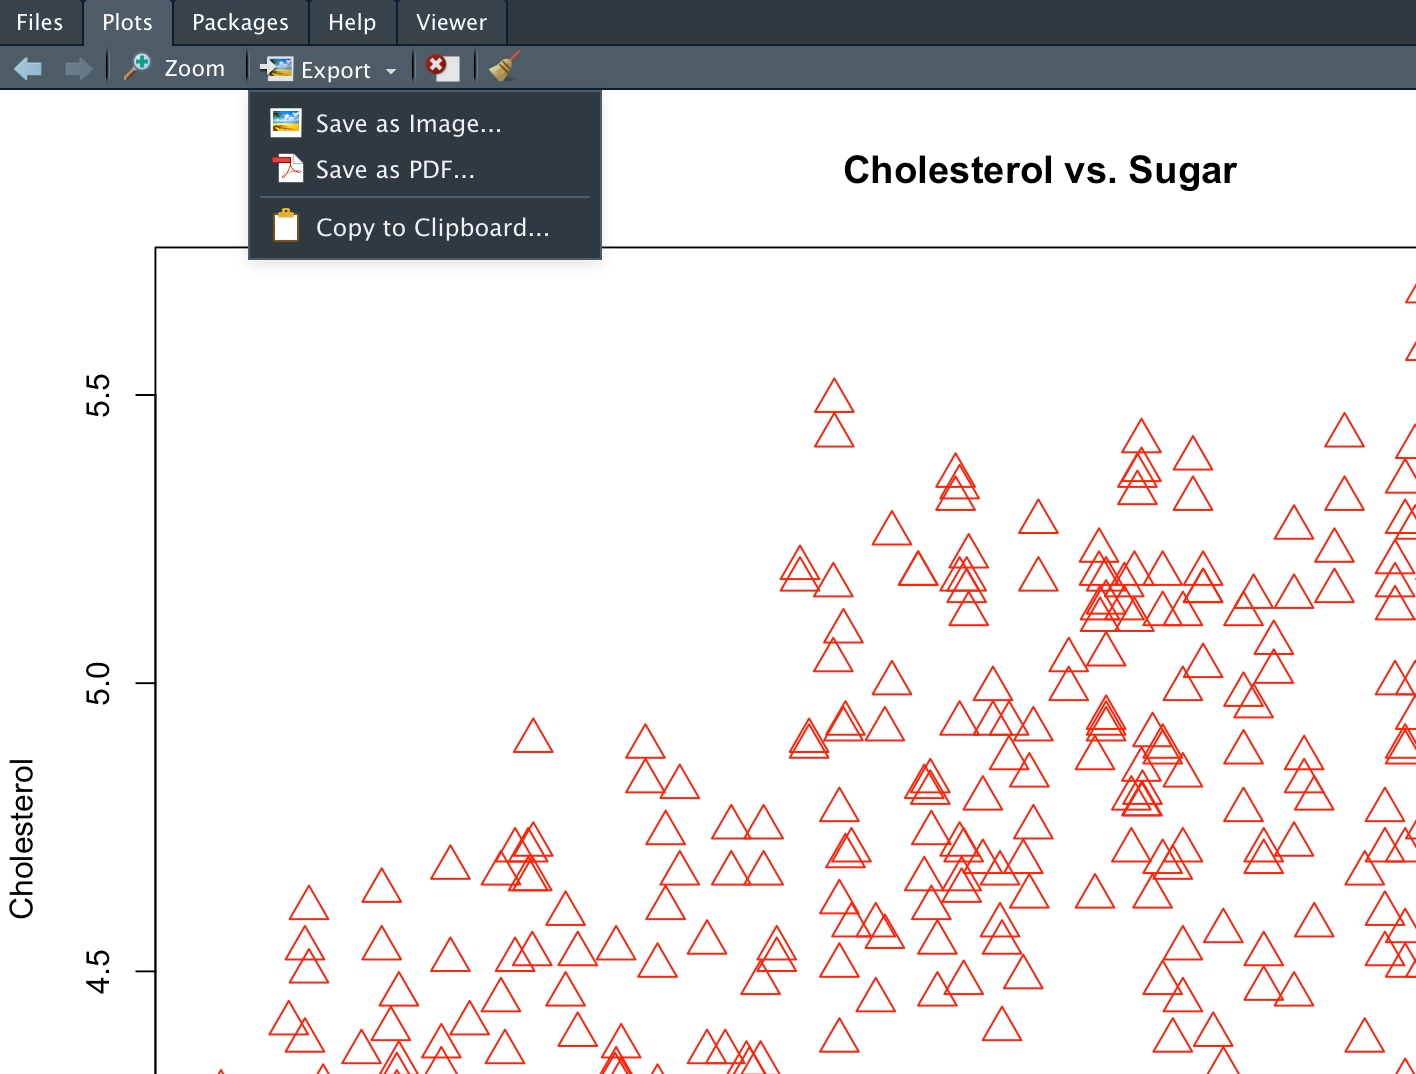
\includegraphics[width=0.7\linewidth]{pics/figure_options} 

}

\caption{Plots Panel Options}\label{fig:unnamed-chunk-533}
\end{figure}

Here are a few options.

\begin{itemize}
\tightlist
\item
  Zoom: the figure will be detached as a separate window in RStudio. You can them drag it around or freely adjust its size just like any other window.
\item
  Export (Save as Image): you can choose the Image Format, change the directory, customize the file name, and set the Width and Height.
\item
  Export (Save as PDF): you can choose the PDF Size, Orientation (Portrait or Landscape), directory, and File Name.
\item
  Export (Copy to Clipboard): this option is useful if you just want to immediately paste the picture into another document such as a Word document, Preview, or email message. Before copying, you can also customize the width and height.
\end{itemize}

In addition to using the menu options, you can also write script to automatically save the plot to your disk. To do that, you need to do the following three steps.

\begin{enumerate}
\def\labelenumi{\arabic{enumi}.}
\tightlist
\item
  Specify a file which will serve as the output device for the \texttt{plot()} function. You can use the functions \texttt{png()}, \texttt{jpeg()}, \texttt{png()}, and \texttt{pdf()} with the target file name as the argument.
\item
  Run the \texttt{plot()} function.
\item
  Run \texttt{dev.off()} to close the connection.
\end{enumerate}

Let's see an example.

\begin{Shaded}
\begin{Highlighting}[]
\FunctionTok{pdf}\NormalTok{(}\StringTok{"data/cholestrol\_vs\_sugar.pdf"}\NormalTok{)}
\FunctionTok{plot}\NormalTok{(gm2004}\SpecialCharTok{$}\NormalTok{sugar,}
\NormalTok{     gm2004}\SpecialCharTok{$}\NormalTok{cholesterol)}
\FunctionTok{dev.off}\NormalTok{()}
\end{Highlighting}
\end{Shaded}

Note that when you use the .pdf format, you can have multiple plots generated from the \texttt{plot()} before running \texttt{dev.off()}. In this case, the output .pdf file will contain multiple pages where each page corresponds to a plot.

\hypertarget{point}{%
\subsection{\texorpdfstring{Using the \texttt{ggplot()} function}{Using the ggplot() function}}\label{point}}

Although the \texttt{plot()} function gets the work done, the \textbf{ggplot2} package provides a superior user experience which allows us to create complex plots with ease. Since the \textbf{ggplot2} package is a member of the \textbf{tidyverse} package, you don't need to install it separately if \textbf{tidyverse} was already installed. Let's first load the package \textbf{ggplot2} and create a scatterplot.

\begin{Shaded}
\begin{Highlighting}[]
\FunctionTok{library}\NormalTok{(ggplot2)}
\FunctionTok{ggplot}\NormalTok{(}\AttributeTok{data =}\NormalTok{ gm2004) }\SpecialCharTok{+} 
  \FunctionTok{geom\_point}\NormalTok{(}\AttributeTok{mapping =} \FunctionTok{aes}\NormalTok{(}\AttributeTok{x =}\NormalTok{ sugar, }
                           \AttributeTok{y =}\NormalTok{ cholesterol))}
\end{Highlighting}
\end{Shaded}

\includegraphics{r02pro_files/figure-latex/unnamed-chunk-535-1.pdf}

Aside from the expected scatterplot, you can see a warning message ``Removed 128 rows containing missing values (geom\_point).'' This indicate that there are 128 rows in \texttt{gm2004} that contains missing values for \texttt{sugar} and/or \texttt{cholesterol} (see Section \ref{missing-values} for a detailed treatment of missing values) and they were removed during the plotting process. The removal of missing values for relevant variables is a default behavior for all plots generated by the \textbf{ggplot2} package.

Now, let's walk through the mechanism of \textbf{ggplot2}. In a nutshell, ggplot2 implements the \textbf{grammar of graphics}, a coherent system for describing and building graphs. A more detailed description on the grammar of graphics can be found in \citet{wickham2010layered}.

Let's break it down into two steps. In \textbf{ggplot2}, we always start with the function \texttt{ggplot()} with a data frame or tibble as its argument.

\begin{Shaded}
\begin{Highlighting}[]
\FunctionTok{ggplot}\NormalTok{(}\AttributeTok{data =}\NormalTok{ gm2004)}
\end{Highlighting}
\end{Shaded}

\includegraphics{r02pro_files/figure-latex/unnamed-chunk-536-1.pdf}

After running this code, you can see an empty plot. This is because ggplot does not yet know which variables or what type of plots you want to create. To generate a \textbf{scatterplot}, you can add a \textbf{layer} using the \texttt{+} operator followed by the \texttt{geom\_point()} function. The \texttt{geom\_point()} is one of the many available \textbf{geoms} in ggplot.

Inside \texttt{geom\_point()}, you need to set the value of the \texttt{mapping} argument. The \texttt{mapping} argument takes a functional form as \texttt{mapping\ =\ aes()}, where the \texttt{aes} is short for \textbf{aesthetics}. For example, you can use \texttt{aes()} to tell ggplot to use which variable on the x-axis and which variable on the y-axis. Let's take another look at this example.

\begin{Shaded}
\begin{Highlighting}[]
\FunctionTok{ggplot}\NormalTok{(}\AttributeTok{data =}\NormalTok{ gm2004) }\SpecialCharTok{+} 
  \FunctionTok{geom\_point}\NormalTok{(}\AttributeTok{mapping =} \FunctionTok{aes}\NormalTok{(}\AttributeTok{x =}\NormalTok{ sugar, }
                           \AttributeTok{y =}\NormalTok{ cholesterol))}
\end{Highlighting}
\end{Shaded}

Here, inside the \texttt{aes()} function, we set \texttt{x\ =\ sugar} and \texttt{y\ =\ cholesterol}, indicating that the variable \texttt{sugar} will appear on the x-axis and \texttt{cholesterol} will appear on the y-axis.

\begin{infobox}{caution}
When creating a ggplot, we recommend starting a new line after each \texttt{+} and also put all arguments of the \texttt{aes()} function on separate lines for better readability.

\end{infobox}

Now, let's look at another example. We would like to explore the relationship between \texttt{GDP\_per\_capita} and \texttt{life\_expectancy}.

\begin{Shaded}
\begin{Highlighting}[]
\FunctionTok{ggplot}\NormalTok{(}\AttributeTok{data =}\NormalTok{ gm2004) }\SpecialCharTok{+} 
  \FunctionTok{geom\_point}\NormalTok{(}\AttributeTok{mapping =} \FunctionTok{aes}\NormalTok{(}\AttributeTok{x =}\NormalTok{ GDP\_per\_capita, }
                           \AttributeTok{y =}\NormalTok{ life\_expectancy))}
\end{Highlighting}
\end{Shaded}

\includegraphics{r02pro_files/figure-latex/unnamed-chunk-538-1.pdf}

We can see that \texttt{life\_expectancy} in general increases (in a non-linear fashion) as \texttt{GDP\_per\_capita} increases, again consistent with our knowledge. From the figure, you can see that there is a pretty heavy left tail for \texttt{GDP\_per\_capita}. To fix this problem, you can actually use a log transformation of \texttt{GDP\_per\_capita} in the scatterplot. Note that you can directly use the transformed form inside the aesthetic mapping, without the need to first add the transformation as a variable.

\begin{Shaded}
\begin{Highlighting}[]
\FunctionTok{ggplot}\NormalTok{(}\AttributeTok{data =}\NormalTok{ gm2004) }\SpecialCharTok{+} 
  \FunctionTok{geom\_point}\NormalTok{(}\AttributeTok{mapping =} \FunctionTok{aes}\NormalTok{(}\AttributeTok{x =} \FunctionTok{log}\NormalTok{(GDP\_per\_capita), }
                           \AttributeTok{y =}\NormalTok{ life\_expectancy))}
\end{Highlighting}
\end{Shaded}

\includegraphics{r02pro_files/figure-latex/unnamed-chunk-539-1.pdf}

After the logarithm transformation, you can see a relationship that is more linear.

\hypertarget{interact-and-save-the-plot-from-ggplot}{%
\subsection{\texorpdfstring{Interact and Save the plot from \texttt{ggplot()}}{Interact and Save the plot from ggplot()}}\label{interact-and-save-the-plot-from-ggplot}}

After generating the plot using \texttt{ggplot()}, you can use exactly the same menu options for interacting the plot as for \texttt{plot()}.

However, the mechanism for saving plots from \texttt{ggplot()} is completely different from that of \texttt{plot()}. To save a plot from \texttt{ggplot()}, you just need to use the \texttt{ggsave()} function after generating the plot without first setting up the connection to the file. The \texttt{ggsave()} function is very smart in the sense that it will automatic save the plot to the desired format depending on the extension of the given file name.

\begin{Shaded}
\begin{Highlighting}[]
\FunctionTok{ggplot}\NormalTok{(}\AttributeTok{data =}\NormalTok{ gm2004) }\SpecialCharTok{+} 
  \FunctionTok{geom\_point}\NormalTok{(}\AttributeTok{mapping =} \FunctionTok{aes}\NormalTok{(}\AttributeTok{x =}\NormalTok{ sugar, }
                           \AttributeTok{y =}\NormalTok{ cholesterol))}
\FunctionTok{ggsave}\NormalTok{(}\StringTok{"data/cholestrol\_vs\_sugar\_ggplot.pdf"}\NormalTok{) }\CommentTok{\#save the plot as a .pdf file}
\FunctionTok{ggsave}\NormalTok{(}\StringTok{"data/cholestrol\_vs\_sugar\_ggplot.jpg"}\NormalTok{) }\CommentTok{\#save the plot as a .jpg image}
\end{Highlighting}
\end{Shaded}

\hypertarget{exercises-31}{%
\subsection{Exercises}\label{exercises-31}}

\begin{enumerate}
\def\labelenumi{\arabic{enumi}.}
\tightlist
\item
  Using the \texttt{sahp} dataset, create a scatterplot to visualize the relationship between \texttt{liv\_area} (on the x-axis) and \texttt{sale\_price} (on the y-axis) without using any package, then set labels according to variable names and change all points to red. Finally, save the plot to \texttt{data/sale\_price\_vs\_liv\_area.jpg} and discuss the findings.
\item
  Using the \texttt{gm2004} dataset, create a scatterplot to visualize the relationship between \texttt{sanitation} ( on the x-axis) and \texttt{life\_expectancy} (on the y-axis) using the \textbf{ggplot2} pckage. Finally, save the plot to \texttt{data/life\_expectancy\_vs\_sanitation.pdf} and discuss the findings.
\end{enumerate}

\hypertarget{aes}{%
\section{ggplot Aesthetics (I): Constant-Valued Aesthetics}\label{aes}}

Having learned how to generate a basic scatterplot using \texttt{geom\_point()} in Section \ref{scatterplot}, let's introduce one of the most important ingredients in a \texttt{geom}, namely, the \textbf{aesthetics}. Aesthetics include various features that you can change that affect the appearances of a plot, including color, shape, and size.

There are in general three kinds of aesthetics:

\begin{enumerate}
\def\labelenumi{\arabic{enumi}.}
\item
  \textbf{Constant-Valued Aesthetics}: this type of aesthetics change the corresponding feature of a plot \textbf{globally} (for example, \texttt{color\ =\ "red"} will make everything red). This type of aesthetic specification appears as \textbf{an argument of the geoms} (for example \texttt{geom\_point()}). This will be the focus of this section.
\item
  \textbf{Local Aesthetics Mapping}: this type of aesthetics will use possibly different values for different data points depending on the \textbf{mapped variable for the current geom}. This type of aesthetic specification appears as an argument of the \texttt{aes()} function of the corresponding geom. We will cover this type of aesthetic in the next Section (Section \ref{aes-map}).
\item
  \textbf{Global Aesthetic Mapping}: this type of aesthetics will use possibly different values for different data points depending on the \textbf{mapped variable at the global level}, which will be \textbf{passed} to all individual geoms. This type of aesthetic specification appears as an argument of the \texttt{aes()} function, which is an argument of the \texttt{ggplot()} function. We will cover this type of aesthetic in Section ???, where multiple geoms are used.
\end{enumerate}

\begin{infobox}{caution}
Note that although we will introduce aesthetics via the example of scatterplot, they are used for all kinds of plots which will be covered at a later time.

\end{infobox}

Let's first review the code we used to generate the scatterplot between \texttt{sugar} and \texttt{cholestrol} in the \texttt{gm2004} dataset.

\begin{Shaded}
\begin{Highlighting}[]
\FunctionTok{library}\NormalTok{(ggplot2)}
\FunctionTok{library}\NormalTok{(r02pro)}
\FunctionTok{ggplot}\NormalTok{(}\AttributeTok{data =}\NormalTok{ gm2004) }\SpecialCharTok{+} 
  \FunctionTok{geom\_point}\NormalTok{(}\AttributeTok{mapping =} \FunctionTok{aes}\NormalTok{(}\AttributeTok{x =}\NormalTok{ sugar, }\AttributeTok{y =}\NormalTok{ cholesterol))}
\end{Highlighting}
\end{Shaded}

\includegraphics{r02pro_files/figure-latex/unnamed-chunk-541-1.pdf}

Now, let's see how to set \textbf{constant-valued aethetics} in \texttt{geom\_point()}.

\textbf{\emph{a. Color}}

To change the color of all points, you can add a \texttt{color} argument in the \texttt{geom\_point()} function. Note that it is placed \textbf{outside} of the \texttt{aes()} function, which is different from aesthetic mappings, to be covered in the next section.

\begin{Shaded}
\begin{Highlighting}[]
\FunctionTok{ggplot}\NormalTok{(}\AttributeTok{data =}\NormalTok{ gm2004) }\SpecialCharTok{+} 
  \FunctionTok{geom\_point}\NormalTok{(}\AttributeTok{mapping =} \FunctionTok{aes}\NormalTok{(}\AttributeTok{x =}\NormalTok{ sugar, }\AttributeTok{y =}\NormalTok{ cholesterol),}
             \AttributeTok{color =} \StringTok{"blue"}\NormalTok{)}
\end{Highlighting}
\end{Shaded}

\includegraphics{r02pro_files/figure-latex/unnamed-chunk-542-1.pdf}

Clearly, all points are changed to blue.

\textbf{\emph{b. Size}}

Similarly, you can set the \texttt{size} aesthetic in the \texttt{geom\_point()} function to change the size of the all points.

\begin{Shaded}
\begin{Highlighting}[]
\FunctionTok{ggplot}\NormalTok{(}\AttributeTok{data =}\NormalTok{ gm2004) }\SpecialCharTok{+} 
  \FunctionTok{geom\_point}\NormalTok{(}\AttributeTok{mapping =} \FunctionTok{aes}\NormalTok{(}\AttributeTok{x =}\NormalTok{ sugar, }\AttributeTok{y =}\NormalTok{ cholesterol),}
             \AttributeTok{size =} \DecValTok{3}\NormalTok{)}
\end{Highlighting}
\end{Shaded}

\includegraphics{r02pro_files/figure-latex/unnamed-chunk-543-1.pdf}

Note that it is very common to set multiple constant valued aesthetic in a geom function.

\begin{Shaded}
\begin{Highlighting}[]
\FunctionTok{ggplot}\NormalTok{(}\AttributeTok{data =}\NormalTok{ gm2004) }\SpecialCharTok{+} 
  \FunctionTok{geom\_point}\NormalTok{(}\AttributeTok{mapping =} \FunctionTok{aes}\NormalTok{(}\AttributeTok{x =}\NormalTok{ sugar, }\AttributeTok{y =}\NormalTok{ cholesterol),}
             \AttributeTok{color =} \StringTok{"blue"}\NormalTok{,}
             \AttributeTok{size =} \DecValTok{3}\NormalTok{)}
\end{Highlighting}
\end{Shaded}

\includegraphics{r02pro_files/figure-latex/unnamed-chunk-544-1.pdf}

You may notice that the points are now bigger than before. Looking at the plot, some points are overlapping with each other, which is sometimes called \textbf{overplotting}. To solve this issue, you can change the transparency level of the points by setting the \texttt{alpha} aesthetic.

\textbf{\emph{c.~Transparency}}

\begin{Shaded}
\begin{Highlighting}[]
\FunctionTok{ggplot}\NormalTok{(}\AttributeTok{data =}\NormalTok{ gm2004) }\SpecialCharTok{+} 
  \FunctionTok{geom\_point}\NormalTok{(}\AttributeTok{mapping =} \FunctionTok{aes}\NormalTok{(}\AttributeTok{x =}\NormalTok{ sugar, }\AttributeTok{y =}\NormalTok{ cholesterol),}
             \AttributeTok{color =} \StringTok{"blue"}\NormalTok{,}
             \AttributeTok{size =} \DecValTok{3}\NormalTok{, }
             \AttributeTok{alpha =} \FloatTok{0.5}\NormalTok{)}
\end{Highlighting}
\end{Shaded}

\includegraphics{r02pro_files/figure-latex/unnamed-chunk-545-1.pdf}

By setting \texttt{alpha\ =\ 0.5}, the points become more visible and the overplotting problem is largely alleviated.

\textbf{\emph{d.~Shape}}

Lastly, we can also change the shape of the points from the default one (circle) to other shapes by the \texttt{shape} argument in \texttt{geom\_point()}.

\begin{Shaded}
\begin{Highlighting}[]
\FunctionTok{ggplot}\NormalTok{(}\AttributeTok{data =}\NormalTok{ gm2004) }\SpecialCharTok{+} 
  \FunctionTok{geom\_point}\NormalTok{(}\AttributeTok{mapping =} \FunctionTok{aes}\NormalTok{(}\AttributeTok{x =}\NormalTok{ sugar, }\AttributeTok{y =}\NormalTok{ cholesterol),}
             \AttributeTok{color =} \StringTok{"blue"}\NormalTok{,}
             \AttributeTok{size =} \DecValTok{3}\NormalTok{, }
             \AttributeTok{alpha =} \FloatTok{0.5}\NormalTok{,}
             \AttributeTok{shape =} \DecValTok{2}\NormalTok{)}
\end{Highlighting}
\end{Shaded}

\includegraphics{r02pro_files/figure-latex/unnamed-chunk-546-1.pdf}

Now, we have all points blue, size of 3, of triangle shape, and of transparency level 0.5. Recall the collection of all shapes is available in Figure \ref{fig:all-shapes}.

You are welcome to try different combinations of global aesthetics.

\hypertarget{exercises-32}{%
\subsection{Exercises}\label{exercises-32}}

\begin{enumerate}
\def\labelenumi{\arabic{enumi}.}
\item
  Using the \texttt{sahp} dataset, create a scatterplot with \textbf{ggplot2} to visualize the relationship between \texttt{lot\_area} (on the x-axis) and \texttt{sale\_price} (on the y-axis) with all points of color purple and size 2.
\item
  Using the \texttt{gm2004} dataset, create a scatterplot with \textbf{ggplot2} to visualize the relationship between \texttt{alcohol} (on the x-axis) and \texttt{liver\_cancer} (on the y-axis) with all points of color pink, size 3, transparency 0.3, and shape diamond.
\end{enumerate}

\hypertarget{aes-map}{%
\section{ggplot Aesthetics (II): Local Aesthetics Mapping}\label{aes-map}}

In Section \ref{aes}, we introduced the first kind of aesthetics, namely \textbf{Constant-Valued Aesthetics}, where we set constant values to aesthetics that change features of the plot globally. In some applications, however, you may want to highlight different groups of the data with different values of aesthetics. In this section, we will dive deep into this topic: \textbf{Local Aesthetics Mapping}.

Believe it or not, we've already seen this kind of aesthetic mapping when we first introduced ggplot in Section \ref{point}.

\begin{Shaded}
\begin{Highlighting}[]
\FunctionTok{library}\NormalTok{(ggplot2)}
\FunctionTok{library}\NormalTok{(r02pro)}
\FunctionTok{ggplot}\NormalTok{(}\AttributeTok{data =}\NormalTok{ gm2004) }\SpecialCharTok{+} 
  \FunctionTok{geom\_point}\NormalTok{(}\AttributeTok{mapping =} \FunctionTok{aes}\NormalTok{(}\AttributeTok{x =}\NormalTok{ sugar, }
                           \AttributeTok{y =}\NormalTok{ cholesterol))}
\end{Highlighting}
\end{Shaded}

\includegraphics{r02pro_files/figure-latex/unnamed-chunk-547-1.pdf}

In the \texttt{aes()} function, \texttt{x} and \texttt{y} can also be viewed as aesthetics. It is clear to see that we are not setting \texttt{x} and \texttt{y} as constants. Instead, we map the variable \texttt{sugar} to \texttt{x} and the variable \texttt{cholesterol} to \texttt{y}. The \texttt{x} and \texttt{y} coordinates control the location of each data points depending on the variables of \texttt{sugar} and \texttt{cholesterol}, which is the essence of scatterplot. Now, let's see how to do local aesthetic mappings for color, size, shape, and so on.

\hypertarget{basic-local-aesthetics-mapping}{%
\subsection{Basic Local Aesthetics Mapping}\label{basic-local-aesthetics-mapping}}

\textbf{\emph{a. Color}}

Let's say you want to use different colors for \texttt{male} and \texttt{female} on the scatterplot. To do this, you can map the discrete variable \texttt{gender} to the \texttt{color} aesthetic by setting \texttt{color\ =\ gender} as an argument in the \texttt{aes()} function.

\begin{Shaded}
\begin{Highlighting}[]
\FunctionTok{ggplot}\NormalTok{(}\AttributeTok{data =}\NormalTok{ gm2004) }\SpecialCharTok{+} 
  \FunctionTok{geom\_point}\NormalTok{(}\AttributeTok{mapping =} \FunctionTok{aes}\NormalTok{(}\AttributeTok{x =}\NormalTok{ sugar, }
                           \AttributeTok{y =}\NormalTok{ cholesterol,}
                           \AttributeTok{color =}\NormalTok{ gender))}
\end{Highlighting}
\end{Shaded}

\includegraphics{r02pro_files/figure-latex/unnamed-chunk-548-1.pdf}

From this figure, we can clearly see that different genders are shown in distinct colors. Also, for the same value of \texttt{sugar}, it appears that the value of \texttt{cholestrol} could be a bit smaller for male than that for female. In addition, \texttt{ggplot()} automatically created a legend to show the correspondence between the gender and colors.

Can we map a continuous variable to the color aesthetic? The answer is positive.

\begin{Shaded}
\begin{Highlighting}[]
\FunctionTok{ggplot}\NormalTok{(}\AttributeTok{data =}\NormalTok{ gm2004) }\SpecialCharTok{+} 
  \FunctionTok{geom\_point}\NormalTok{(}\AttributeTok{mapping =} \FunctionTok{aes}\NormalTok{(}\AttributeTok{x =}\NormalTok{ sugar, }
                           \AttributeTok{y =}\NormalTok{ cholesterol,}
                           \AttributeTok{color =}\NormalTok{ population))}
\end{Highlighting}
\end{Shaded}

\includegraphics{r02pro_files/figure-latex/scatterplot-color-1.pdf}

Here, you can see that the color of the points changes smoothly according to the value of \texttt{population}, the details of which is shown in the legend. In particular, the darker points represent smaller populations while the lighter ones correspond to bigger populations.

\textbf{\emph{b. Size}}

In addition to color, you can also map a discrete variable to the size aesthetic.

\begin{Shaded}
\begin{Highlighting}[]
\FunctionTok{ggplot}\NormalTok{(}\AttributeTok{data =}\NormalTok{ gm2004) }\SpecialCharTok{+} 
  \FunctionTok{geom\_point}\NormalTok{(}\AttributeTok{mapping =} \FunctionTok{aes}\NormalTok{(}\AttributeTok{x =}\NormalTok{ sugar, }
                           \AttributeTok{y =}\NormalTok{ cholesterol,}
                           \AttributeTok{size =}\NormalTok{ gender),}
             \AttributeTok{alpha =} \FloatTok{0.5}\NormalTok{)}
\end{Highlighting}
\end{Shaded}

\includegraphics{r02pro_files/figure-latex/unnamed-chunk-549-1.pdf}

You can see from the plot that the sizes of the points are now different according to the \texttt{gender}.

To alleviate the overplotting issue, we added a \textbf{contant-valued aesthetic} \texttt{alpha\ =\ 0.5} to the \texttt{geom\_point()} function, making all points more transparent. Please pay close attention to the location where we put the argument:

\begin{enumerate}
\def\labelenumi{\arabic{enumi}.}
\tightlist
\item
  Contant-Valued Aesthetic: the aesthetic specification is put inside the \texttt{geom\_point()} function.
\item
  Local Aesthetics Mapping: the aesthetic mapping is put inside the \texttt{aes()} function, which is itself an argument of the \texttt{geom\_point()} function.
\end{enumerate}

There is a warning message: ``Using size for a discrete variable is not advised.'' The reason is that different sizes may implicitly indicate a particular ordering of the groups, which are usually not clear for a discrete variable.

Now, let's try to map a continuous variable \texttt{BMI} to the size aesthetic.

\begin{Shaded}
\begin{Highlighting}[]
\FunctionTok{ggplot}\NormalTok{(}\AttributeTok{data =}\NormalTok{ gm2004) }\SpecialCharTok{+} 
  \FunctionTok{geom\_point}\NormalTok{(}\AttributeTok{mapping =} \FunctionTok{aes}\NormalTok{(}\AttributeTok{x =}\NormalTok{ sugar, }
                           \AttributeTok{y =}\NormalTok{ cholesterol,}
                           \AttributeTok{size =}\NormalTok{ BMI),}
             \AttributeTok{alpha =} \FloatTok{0.5}\NormalTok{)}
\end{Highlighting}
\end{Shaded}

\includegraphics{r02pro_files/figure-latex/unnamed-chunk-550-1.pdf}

Note that now the size of the points changes according to the corresponding \texttt{BMI} value, i.e.~the larger points represent large BMIs values and the smaller ones correspond to smaller BMI values. It is worth noting that the legend only shows three representative \texttt{BMI} values (20, 25, an 30) and their corresponding sizes, however, we have other sizes depending on exact BMI values.

\textbf{\emph{c.~Shape}}

We can also map a discrete variable to the \texttt{shape} aesthetic.

\begin{Shaded}
\begin{Highlighting}[]
\FunctionTok{ggplot}\NormalTok{(}\AttributeTok{data =}\NormalTok{ gm2004) }\SpecialCharTok{+} 
  \FunctionTok{geom\_point}\NormalTok{(}\AttributeTok{mapping =} \FunctionTok{aes}\NormalTok{(}\AttributeTok{x =}\NormalTok{ sugar, }
                           \AttributeTok{y =}\NormalTok{ cholesterol,}
                           \AttributeTok{shape =}\NormalTok{ continent))}
\end{Highlighting}
\end{Shaded}

\includegraphics{r02pro_files/figure-latex/unnamed-chunk-551-1.pdf}

Now, the shape of the points are different for each continent.

Can we map a continuous variable to the shape aesthetic? Let's try it out.

\begin{Shaded}
\begin{Highlighting}[]
\FunctionTok{ggplot}\NormalTok{(}\AttributeTok{data =}\NormalTok{ gm2004) }\SpecialCharTok{+} 
  \FunctionTok{geom\_point}\NormalTok{(}\AttributeTok{mapping =} \FunctionTok{aes}\NormalTok{(}\AttributeTok{x =}\NormalTok{ sugar, }
                           \AttributeTok{y =}\NormalTok{ cholesterol,}
                           \AttributeTok{shape =}\NormalTok{ BMI))}
\end{Highlighting}
\end{Shaded}

You will see an error message: ``A continuous variable can not be mapped to shape''. This is because shape is of a discrete nature in the sense that different shapes have no natural ordering and the number of possible shapes is finite where the continuous variable could take infinitely many different values.

\hypertarget{customize-the-local-aesthetics-mapping}{%
\subsection{Customize the Local Aesthetics Mapping}\label{customize-the-local-aesthetics-mapping}}

So far, we have introduced the basic local aesthetics mapping, where the default aesthetic values are used. Sometimes, you may want to use specific aesthetic values (colors, shapes) for particular values of the mapped variable.

\textbf{\emph{a. Customize color for discrete variables}}

Let's start with the color aesthetic. To customize the colors with discrete variable, you can add a layer to the ggplot with function \texttt{scale\_colour\_manual} with argument \texttt{values} containing a character vector consisting of the colors.

\begin{Shaded}
\begin{Highlighting}[]
\FunctionTok{ggplot}\NormalTok{(}\AttributeTok{data =}\NormalTok{ gm2004) }\SpecialCharTok{+} 
  \FunctionTok{geom\_point}\NormalTok{(}\AttributeTok{mapping =} \FunctionTok{aes}\NormalTok{(}\AttributeTok{x =}\NormalTok{ sugar, }
                           \AttributeTok{y =}\NormalTok{ cholesterol,}
                           \AttributeTok{color =}\NormalTok{ gender)) }\SpecialCharTok{+} 
  \FunctionTok{scale\_colour\_manual}\NormalTok{(}\AttributeTok{values =} \FunctionTok{c}\NormalTok{(}\StringTok{"orange"}\NormalTok{,}\StringTok{"purple"}\NormalTok{))}
\end{Highlighting}
\end{Shaded}

\includegraphics{r02pro_files/figure-latex/unnamed-chunk-553-1.pdf}

Now, the female group has color orange and the male group has color purple.

\textbf{\emph{b. Remove missing values}}

Let's try to map \texttt{continent} to \texttt{color}.

\begin{Shaded}
\begin{Highlighting}[]
\FunctionTok{ggplot}\NormalTok{(}\AttributeTok{data =}\NormalTok{ gm2004) }\SpecialCharTok{+} 
  \FunctionTok{geom\_point}\NormalTok{(}\AttributeTok{mapping =} \FunctionTok{aes}\NormalTok{(}\AttributeTok{x =}\NormalTok{ sugar, }
                           \AttributeTok{y =}\NormalTok{ cholesterol,}
                           \AttributeTok{color =}\NormalTok{ continent))}
\end{Highlighting}
\end{Shaded}

\includegraphics{r02pro_files/figure-latex/unnamed-chunk-554-1.pdf}

The plot shows us the Africa countries in general have a lower value of \texttt{sugar} as well as a small value of \texttt{cholestrol}. On the other hand, the American and European countries have large values of \texttt{sugar} and \texttt{cholestrol}.

You may noticed that this is a level \texttt{NA} for the continent due to missing values. To address this issue, you can use the \texttt{remove\_missing()} function to remove observations with a missing value of \texttt{continent}.

\begin{Shaded}
\begin{Highlighting}[]
\FunctionTok{ggplot}\NormalTok{(}\AttributeTok{data =} \FunctionTok{remove\_missing}\NormalTok{(gm2004, }\AttributeTok{vars =} \StringTok{"continent"}\NormalTok{)) }\SpecialCharTok{+} 
  \FunctionTok{geom\_point}\NormalTok{(}\AttributeTok{mapping =} \FunctionTok{aes}\NormalTok{(}\AttributeTok{x =}\NormalTok{ sugar, }
                           \AttributeTok{y =}\NormalTok{ cholesterol,}
                           \AttributeTok{color =}\NormalTok{ continent))}
\end{Highlighting}
\end{Shaded}

\includegraphics{r02pro_files/figure-latex/unnamed-chunk-555-1.pdf}

Now, only the five continents are displayed.

\begin{infobox}{caution}
Note that here, we add the argument \texttt{vars\ =\ "continent"} in the \texttt{remove\_missing()} function. This works by removing the observations only if the \texttt{continent} variable is missing. Without such an argument, an observation will be removed as long as at least one variable is missing. For a dataset like \texttt{gm2004} that contain multiple variables, we recommend explicitly specify the variables that need to be considered for missingness. Here, the \texttt{vars} can take the value of a character vector, containing all variables that you want to consider for missingness.

\end{infobox}

\textbf{\emph{c.~Customize color for continuous variables}}

To customize the color for continuous variables, you can add a layer \texttt{scale\_color\_continuous()} which specify the lower-value color and the high-value color for the variable.

\begin{Shaded}
\begin{Highlighting}[]
\FunctionTok{ggplot}\NormalTok{(}\AttributeTok{data =}\NormalTok{ gm2004) }\SpecialCharTok{+} 
  \FunctionTok{geom\_point}\NormalTok{(}\AttributeTok{mapping =} \FunctionTok{aes}\NormalTok{(}\AttributeTok{x =}\NormalTok{ sugar, }
                           \AttributeTok{y =}\NormalTok{ cholesterol,}
                           \AttributeTok{color =}\NormalTok{ BMI)) }\SpecialCharTok{+} 
  \FunctionTok{scale\_color\_continuous}\NormalTok{(}\AttributeTok{low =} \StringTok{"green"}\NormalTok{, }
                         \AttributeTok{high =} \StringTok{"red"}\NormalTok{)}
\end{Highlighting}
\end{Shaded}

\includegraphics{r02pro_files/figure-latex/color-discrete-customize-1.pdf}

Now, we mapped the \texttt{BMI} to the color aesthetic and the lower values of \texttt{BMI} are mapped to green while the higher values are mapped to red.

\textbf{\emph{d.~Customize the shape for discrete variables}}

Similarly, you can also customize the shapes for each level of the discrete variable.

\begin{Shaded}
\begin{Highlighting}[]
\FunctionTok{ggplot}\NormalTok{(}\AttributeTok{data =}\NormalTok{ gm2004) }\SpecialCharTok{+} 
  \FunctionTok{geom\_point}\NormalTok{(}\AttributeTok{mapping =} \FunctionTok{aes}\NormalTok{(}\AttributeTok{x =}\NormalTok{ sugar, }
                           \AttributeTok{y =}\NormalTok{ cholesterol,}
                           \AttributeTok{shape =}\NormalTok{ gender)) }\SpecialCharTok{+}
  \FunctionTok{scale\_shape\_manual}\NormalTok{(}\AttributeTok{values =} \FunctionTok{c}\NormalTok{(}\DecValTok{6}\NormalTok{, }\DecValTok{3}\NormalTok{))}
\end{Highlighting}
\end{Shaded}

\includegraphics{r02pro_files/figure-latex/unnamed-chunk-556-1.pdf}

Here, we have the female and male being mapped to shape 6 and 3, respectively. Recall that all possible shapes are shown in Figure \ref{fig:all-shapes}.

\hypertarget{customize-the-legend-order-for-discrete-variables}{%
\subsection{Customize the legend order for discrete variables}\label{customize-the-legend-order-for-discrete-variables}}

Let's review the following plot

\begin{Shaded}
\begin{Highlighting}[]
\FunctionTok{ggplot}\NormalTok{(}\AttributeTok{data =} \FunctionTok{remove\_missing}\NormalTok{(gm2004, }\AttributeTok{vars =} \StringTok{"continent"}\NormalTok{)) }\SpecialCharTok{+} 
  \FunctionTok{geom\_point}\NormalTok{(}\AttributeTok{mapping =} \FunctionTok{aes}\NormalTok{(}\AttributeTok{x =}\NormalTok{ sugar, }
                           \AttributeTok{y =}\NormalTok{ cholesterol,}
                           \AttributeTok{color =}\NormalTok{ continent))}
\end{Highlighting}
\end{Shaded}

\includegraphics{r02pro_files/figure-latex/unnamed-chunk-557-1.pdf}

Looking at the legend, you can see that different \texttt{continent} values are in alphabetical order as introduced in Section \ref{character-sort-rank-order} when you learned the ordering of character vectors. Sometimes, you may want to arrange these values in a different order in the plot. To achieve this, you can use the \texttt{factor()} function with the argument \texttt{levels} which specifies the desired order.

\begin{Shaded}
\begin{Highlighting}[]
\FunctionTok{ggplot}\NormalTok{(}\AttributeTok{data =} \FunctionTok{remove\_missing}\NormalTok{(gm2004, }\AttributeTok{vars =} \StringTok{"continent"}\NormalTok{)) }\SpecialCharTok{+} 
  \FunctionTok{geom\_point}\NormalTok{(}\AttributeTok{mapping =} \FunctionTok{aes}\NormalTok{(}\AttributeTok{x =}\NormalTok{ sugar, }
                           \AttributeTok{y =}\NormalTok{ cholesterol,}
                           \AttributeTok{color =} \FunctionTok{factor}\NormalTok{(continent,}
                                          \FunctionTok{c}\NormalTok{(}\StringTok{"Oceania"}\NormalTok{, }\StringTok{"Europe"}\NormalTok{, }\StringTok{"Asia"}\NormalTok{, }\StringTok{"Americas"}\NormalTok{,}\StringTok{"Africa"}\NormalTok{))))}
\end{Highlighting}
\end{Shaded}

\includegraphics{r02pro_files/figure-latex/unnamed-chunk-558-1.pdf}

\hypertarget{exercises-33}{%
\subsection{Exercises}\label{exercises-33}}

\begin{enumerate}
\def\labelenumi{\arabic{enumi}.}
\item
  Using the \texttt{sahp} dataset, create a scatterplot to visualize the relationship between \texttt{area} (on the x-axis) and \texttt{sale\_price} (on the y-axis) using ggplot,
\item
  Using the \texttt{gm2004} dataset, create a scatterplot to visualize the relationship between \texttt{alcohol} (on the x-axis) and \texttt{liver\_cancer} (on the y-axis) where the points are purple and the size of the points are determined by the \texttt{BMI} values using the \textbf{ggplot2} package.
\end{enumerate}

  \bibliography{book.bib,packages.bib}

\end{document}
